% Bachelor thesis: Tactical Eye
% Built on the official ELTE Faculty of Informatics template (elteikthesis.cls,
% MIT licence, see LICENSE-elteikthesis).
%
% Build the PDF (from this folder):
%     latexmk -pdf thesis.tex
% latexmk runs pdflatex and biber as many times as needed, so references,
% the bibliography and the lists of figures/tables come out right.
\documentclass[
	%twoside, % double sided printing
	%draft,   % quicker build without images
	%final,   % hides the todo notes
]{elteikthesis}[2024/04/26]

% Document's metadata
\title{Tactical Eye: Automated Video Analytics \& Tactical Visualization Platform}
\date{2026} % year of defence

% Author's metadata
\author{Mudassir Ahmed Chaudhry}
\degree{Computer Science BSc}

% Supervisor's metadata
\supervisor{Gaál Bence}
\affiliation{Assistant Professor}

% University's metadata
\university{Eötvös Loránd University}
\faculty{Faculty of Informatics}
\department{Department of Media and\\Educational Technology}
\city{Budapest}
\logo{elte_cimer_szines}

% Extra packages on top of the template
\usepackage{pdflscape} % landscape pages for the large diagrams
\usepackage{amssymb}   % \checkmark and other symbols
\usepackage{xurl}      % long URLs may break anywhere

% Long lines in code listings (commands, URLs) wrap instead of running into the margin
\lstset{breaklines=true, breakatwhitespace=false, columns=fullflexible, keepspaces=true}
% Shell commands and configuration files: no syntax colouring
\lstdefinestyle{plain}{language={}}
% The template's listings know Python but not TypeScript
\lstdefinelanguage{TypeScript}{
	morekeywords={const, let, function, return, if, else, async, await, export,
		import, from, new, true, false, null, undefined, interface, type, for, of},
	sensitive=true,
	morecomment=[l]{//},
	morecomment=[s]{/*}{*/},
	morestring=[b]",
	morestring=[b]',
}

% Bibliography
\addbibresource{references.bib}

% Figures are looked up in these folders
\graphicspath{{images/}{figures/}{screenshots/}}
% Slightly taller table rows so tables are easier to read
\renewcommand{\arraystretch}{1.25}

\begin{document}
\documentlang{english}
% Cross-references print "Chapter 2" and "Section 3.8" with a capital letter.
% This must come after \documentlang, which resets the names to lower case.
\renewcommand{\chapterautorefname}{Chapter}
\renewcommand{\sectionautorefname}{Section}
\renewcommand{\subsectionautorefname}{Section}
\renewcommand{\subsubsectionautorefname}{Section}

% List of todos (hidden with the "final" option)
%\listoftodos[\todolabel]

\maketitle
% The topic declaration form is attached separately.

\tableofcontents
\cleardoublepage

\chapter{Introduction}
\label{ch:introduction}

\section{Motivation}

A youth or amateur coach who wants to know how compact the team stayed in the second half, or which shape the opponent defended in, has two options today. One is to buy data: top clubs get tracking data from multi-camera systems in the stadium, from GPS vests, or from providers whose operators annotate every match by hand. The other is to watch the video again with a notepad. The first is out of reach below professional level, and the second takes hours and produces no numbers.

What these coaches usually do have is video. The question I started from was therefore a practical one: how much of the professional tactical picture (positions in metres, team shape, formations, running distances) can be recovered automatically from a single broadcast camera, and how can it be shown so that a coach actually uses it?

Off-the-shelf tools did not answer this. Commercial platforms sell their data per match and do not analyse the user's own footage. The open-source football examples, such as the Roboflow \emph{sports} repository~\cite{roboflowsports}, are notebooks that draw boxes on a clip; they do not run as a service, do not survive a crash halfway through a 45-minute video, and have no interface for a coach. I wanted a system that a non-technical user could open in a browser, upload a match to, and come back to later.

The computer vision part has become feasible: YOLOv8~\cite{yolov8} detects players and the ball, ByteTrack~\cite{bytetrack} follows them over time, and projective geometry~\cite{hartley} maps the image onto a flat pitch. The engineering part was at least as demanding. On my laptop a 30-second clip took about 25 minutes to analyse, so the analysis could never run inside a web request, and the results are only useful when they are drawn on the video they came from, frame by frame, while the camera pans.

\section{Objectives and overview}

The aim was to build \textbf{Tactical Eye}, a web platform that turns football video into tactical information without manual annotation. A user uploads a match, follows the analysis live, and then watches the video with every player marked by their position, movement paths, team shapes and heatmaps drawn on the pitch, next to a 2D tactical board, the formations of both teams, statistics and an AI-written coaching report (\autoref{fig:intro-analysis}).

\begin{figure}[htbp]
	\centering
	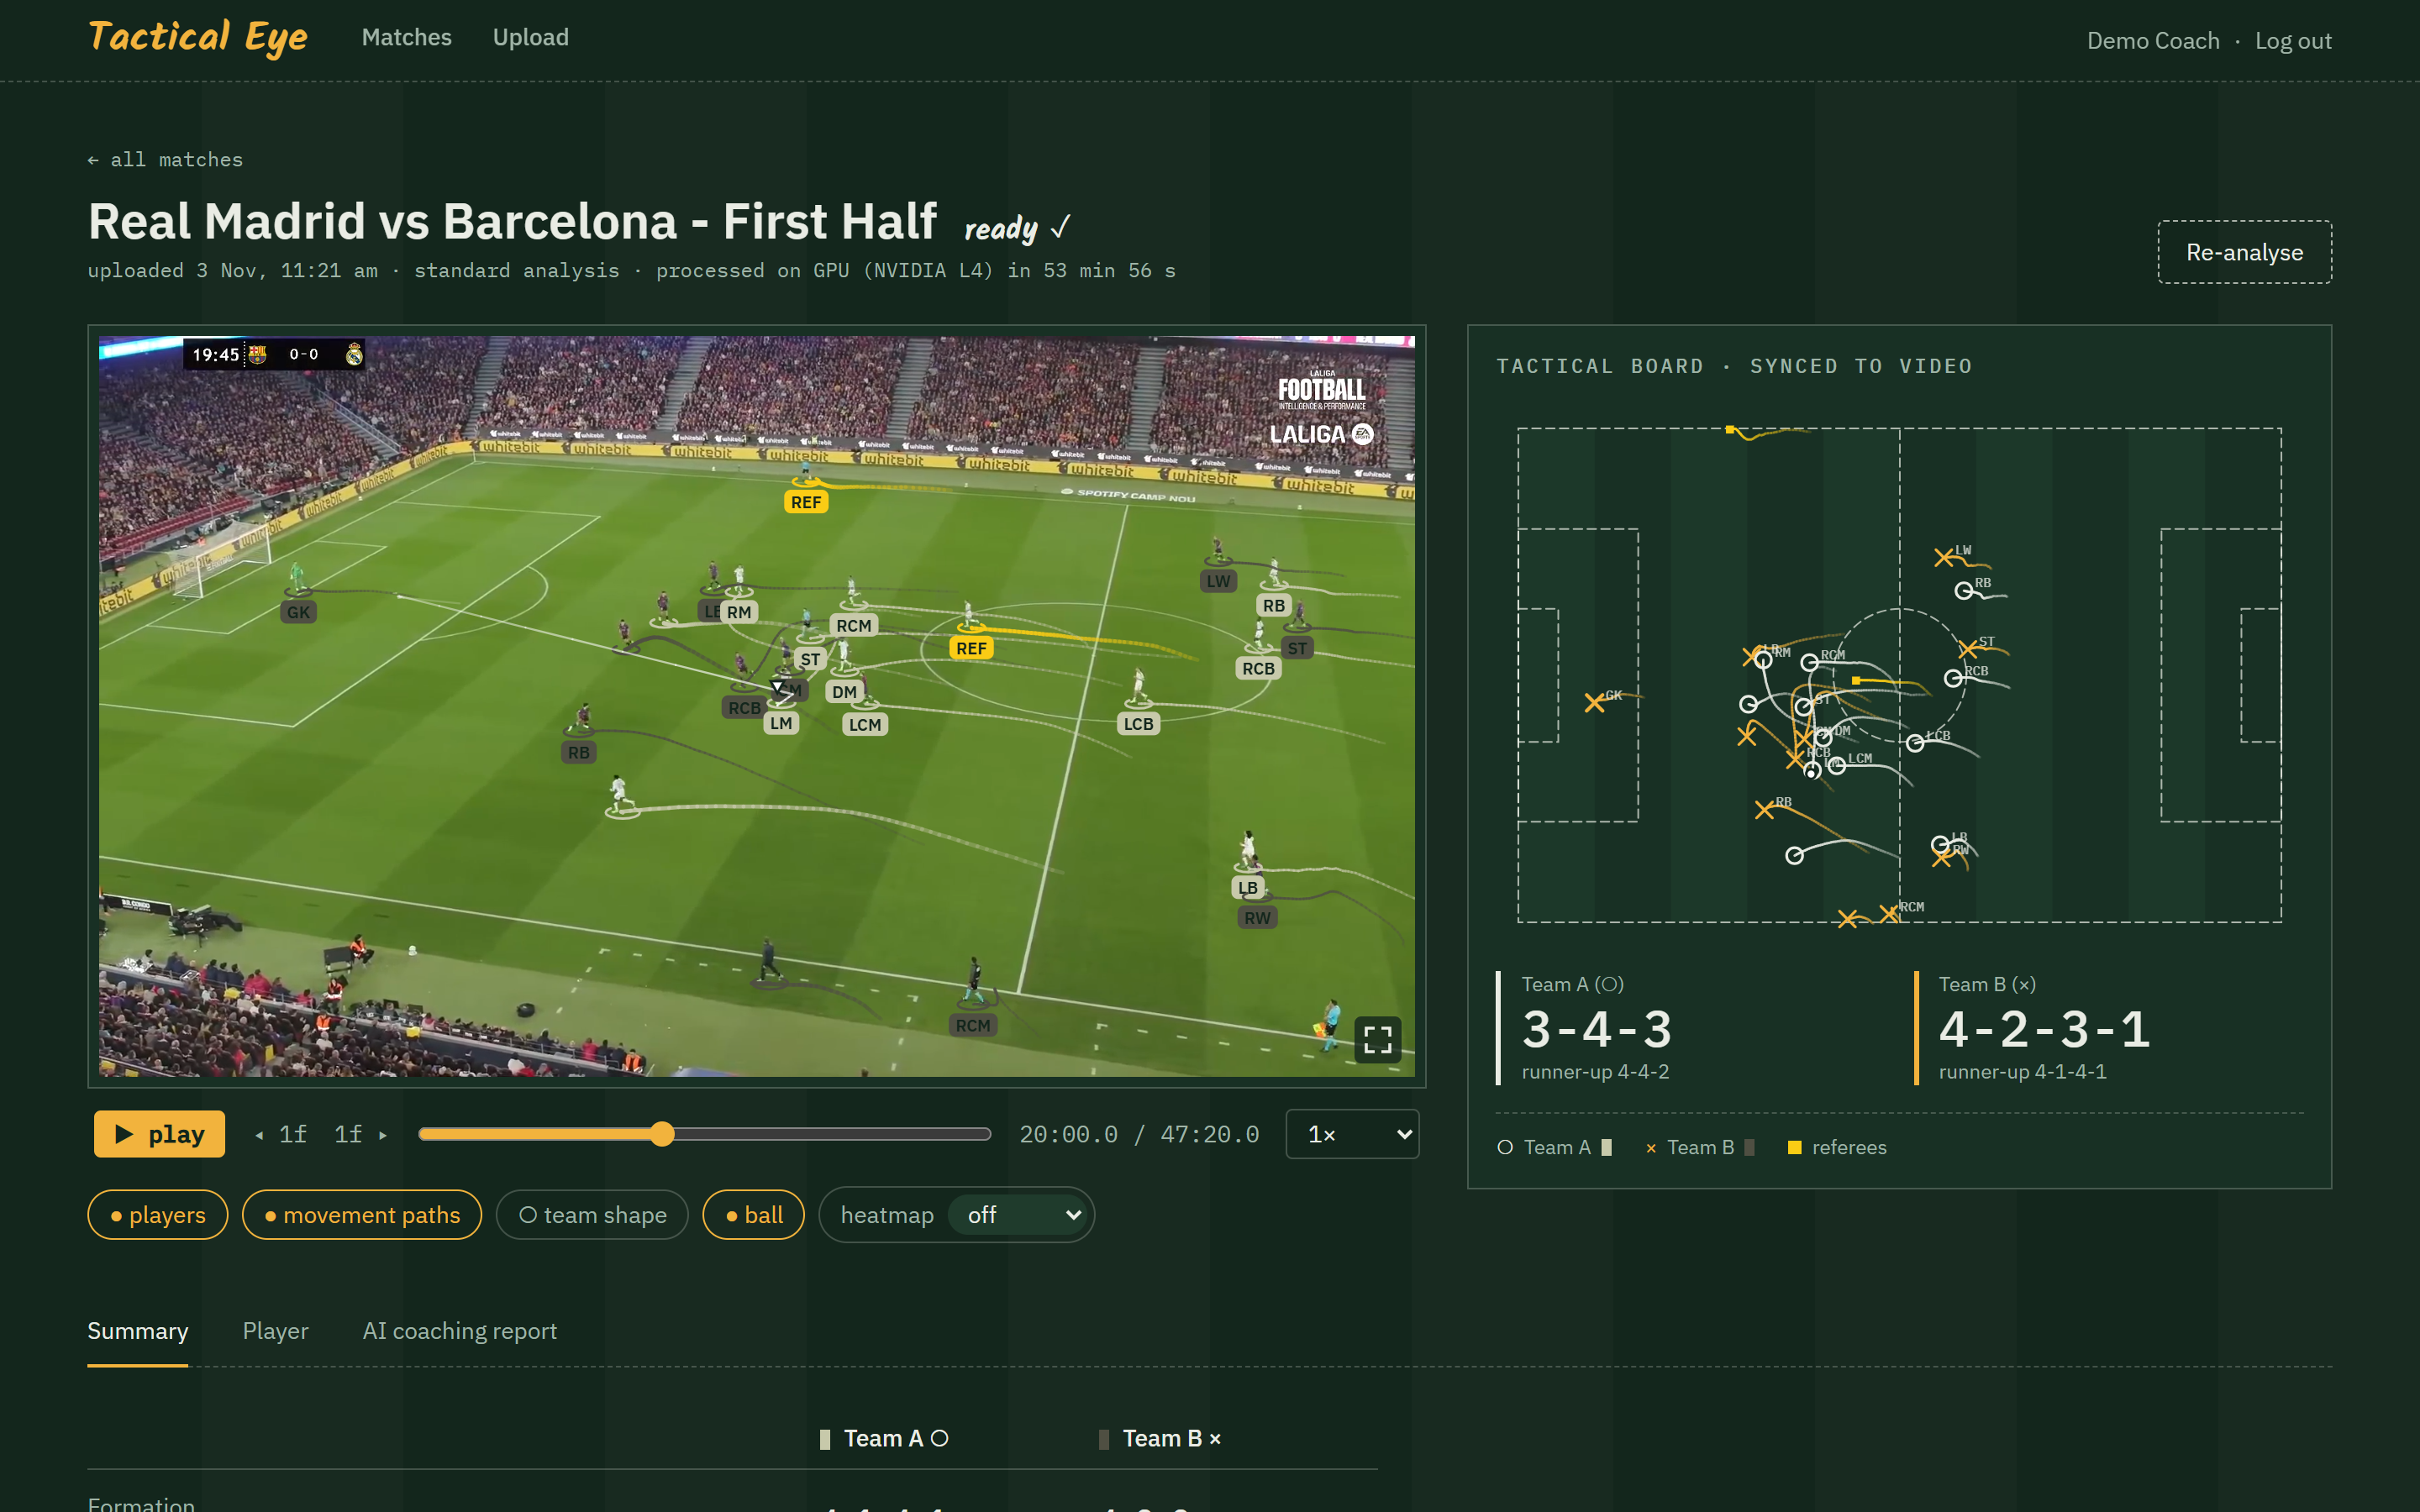
\includegraphics[width=\textwidth]{11_match_page}
	\caption{The analysis page of a full half: video overlays, tactical board and the formations of both teams}
	\label{fig:intro-analysis}
\end{figure}

The platform is a distributed system of four services. A React dashboard runs in the browser; a Node.js API handles accounts and uploads and puts analysis jobs on a Redis queue; a Python AI worker takes the jobs and runs the computer vision pipeline, optionally on a rented cloud GPU; and the API can ask a language model on Azure OpenAI to write the report. Every service runs in a Docker container, and a CI/CD pipeline tests the code and publishes the images.

The platform works from a single broadcast camera, so it only sees what the camera shows. It measures positions, movement and shape, not events such as passes or shots, and because players keep leaving the picture it labels them by position (left back, striker\dots) instead of by name. I tested it on five 30-second Bundesliga clips~\cite{dfl} and on two full halves of about 48 minutes each.

\section{Structure of the thesis}

\autoref{ch:user} is the user documentation: what the software is for, what it needs, how to install it, and every function of the dashboard with its messages. \autoref{ch:developer} is the developer documentation: requirements, architecture, data design, the analysis pipeline, the modules and the main implementation decisions. \autoref{ch:testing} describes the automated tests, the accuracy check against hand-annotated frames and the runs on full halves. \autoref{ch:conclusion} closes with what I learnt.

\cleardoublepage

\chapter{User documentation}
\label{ch:user}

This chapter is for the people who use Tactical Eye: coaches and analysts who upload and study matches, and the operator who installs and runs the platform. It explains what the software does, what it needs, how to install and start it, and how to use every part of the dashboard. The last section lists the messages the system can show and what to do about each of them.

\section{What Tactical Eye is for}

Tactical Eye turns football match video into tactical information without manual annotation. The user uploads a recording from a broadcast-style camera, the wide view of the pitch that pans to follow play, either a short clip or a full half. The platform finds every player, goalkeeper, referee and the ball, follows them through the video and converts their positions from the camera image into pitch coordinates in metres. It decides from the shirt colours which players belong to which team, recognises each team's formation (for example 4-4-2 or 5-3-2) and how it changes, and labels every player with the position they play in that formation, such as LB for left back or ST for striker.

From these trajectories it measures how compact, wide and deep each team is, how far and how fast each position ran, and where each team and the ball spent their time. Everything is drawn on top of the original video, so the user watches the match and sees its structure at the same time. A 2D tactical board shows the same moment from above, and an AI-written coaching report summarises the numbers in plain language.

\section{Target audience and user levels}

The intended users are coaches, video analysts and scouts of amateur and youth clubs, students of the game, and anyone with match video but no access to commercial tracking data. The dashboard runs in an ordinary web browser and needs no technical knowledge. \autoref{tab:user-levels} lists the three kinds of user.

\begin{table}[H]
	\centering
	\begin{tabular}{|p{0.22\textwidth}|p{0.70\textwidth}|}
		\hline
		\textbf{User level} & \textbf{What they can do} \\
		\hline
		Visitor (not logged in) & Open the login page, create an account, log in. Every other page sends a visitor to the login page. \\
		\hline
		Registered user & Upload matches, follow the analysis live, cancel it, list their own matches, watch the interactive analysis, inspect positions, read the summary, generate the AI coaching report, re-analyse and delete their own matches, log out. A user only ever sees their own matches. \\
		\hline
		Operator & Installs and runs the platform (\autoref{sec:installation}), sets up the optional cloud GPU and the AI report service, and watches the health of the system. The operator works on the server, not in the dashboard. \\
		\hline
	\end{tabular}
	\caption{User levels}
	\label{tab:user-levels}
\end{table}

There is no administrator role inside the dashboard. Each user manages their own data, and the platform has no shared content that would need moderation.

\section{System requirements}

Users only need a browser (\autoref{tab:client-req}). The server, which can be the same computer, for example a laptop used for a demonstration, runs the services (\autoref{tab:server-req}).

\begin{table}[H]
	\centering
	\begin{tabular}{|p{0.15\textwidth}|p{0.38\textwidth}|p{0.38\textwidth}|}
		\hline
		& \textbf{Minimum} & \textbf{Recommended} \\
		\hline
		Browser & Current Chrome, Edge, Firefox or Safari with HTML5 video, WebSocket and Fullscreen support & Latest Chrome or Edge, which report the exact frame on screen and so keep the overlays frame-accurate (\autoref{sec:overlay-sync}) \\
		\hline
		Screen & $1280 \times 720$; the layout also adapts to tablets & $1920 \times 1080$ or larger \\
		\hline
		Network & Access to the server & Fast connection for uploading full halves (about 0.5\,GB each) \\
		\hline
	\end{tabular}
	\caption{Requirements on the user's side}
	\label{tab:client-req}
\end{table}

\begin{table}[H]
	\centering
	\begin{tabular}{|p{0.15\textwidth}|p{0.38\textwidth}|p{0.38\textwidth}|}
		\hline
		& \textbf{Minimum} & \textbf{Recommended} \\
		\hline
		Operating system & Windows 10/11, macOS or Linux that runs Docker & Linux server, or Windows 11 with WSL 2 \\
		\hline
		Software & Docker Desktop, or Docker Engine with Compose v2 & The same, plus Git for downloading and updating the code \\
		\hline
		Processor & 4-core x86-64 CPU & 8 or more cores, or an NVIDIA GPU, locally or as the cloud GPU service \\
		\hline
		Memory & 8\,GB RAM & 16\,GB RAM; analysing a full half used up to 4.4\,GB \\
		\hline
		Disk & 15\,GB free: Docker images about 4\,GB, AI models 270\,MB, plus videos & 50\,GB or more; one analysed half needs about 1.2\,GB for the playback copy and 54\,MB for its results \\
		\hline
		Network & Internet access while building the images & Internet access for the optional cloud GPU and AI report \\
		\hline
	\end{tabular}
	\caption{Requirements on the server}
	\label{tab:server-req}
\end{table}

The analysis is heavy. On the development laptop (Intel Core i7-1255U, 8\,GB RAM) a 30-second clip takes about 25 minutes in Standard mode, and a full half is not practical. On a rented NVIDIA L4 GPU the same clip takes about 40 seconds and a 47-minute half about 54 minutes (\autoref{sec:long-videos}). The platform works on modest hardware; it is simply slow there.

\section{Installation and start-up}
\label{sec:installation}

The whole platform starts with one Docker command. Docker downloads and builds everything else, so no programming tools are needed on the server.

\subsection{Getting the software and the AI models}

\begin{enumerate}
	\item Install \textbf{Docker Desktop} from \url{https://www.docker.com} and start it. On Windows, accept the installation of WSL 2 when asked.
	\item Download the source code, either as a ZIP file from the GitHub repository or with Git:
\begin{lstlisting}[style=plain]
git clone https://github.com/mudassir709/Football-AI-tactical-Analyst.git
cd Football-AI-tactical-Analyst
\end{lstlisting}
	\item Download the two pretrained AI models (270\,MB together) and save them in the folder \texttt{worker/models/} under exactly these names. They are not part of the repository because of their size.
	\begin{itemize}
		\item \texttt{football-player-detection.\allowbreak{}pt}, the detector of players, goalkeepers, referees and the ball:\\
		\url{https://drive.google.com/uc?id=17PXFNlx-jI7VjVo_vQnB1sONjRyvoB-q}
		\item \texttt{football-pitch-detection.\allowbreak{}pt}, the detector of the 32 pitch landmarks:\\
		\url{https://drive.google.com/uc?id=1Ma5Kt86tgpdjCTKfum79YMgNnSjcoOyf}
	\end{itemize}
	The links open in a browser. On a server without a browser, the \texttt{gdown} tool downloads them directly:
\begin{lstlisting}[style=plain]
pip install gdown
gdown -O worker/models/football-player-detection.pt "https://drive.google.com/uc?id=17PXFNlx-jI7VjVo_vQnB1sONjRyvoB-q"
gdown -O worker/models/football-pitch-detection.pt "https://drive.google.com/uc?id=1Ma5Kt86tgpdjCTKfum79YMgNnSjcoOyf"
\end{lstlisting}
\end{enumerate}

\subsection{Configuration}

The settings live in a file called \texttt{.\allowbreak{}env} in the main folder. Copy the template \texttt{.\allowbreak{}env.\allowbreak{}example} to \texttt{.\allowbreak{}env} and edit the values in a text editor; \autoref{tab:env} explains each one. The file holds passwords and keys, so it must never be shared or uploaded, and the repository is set up to ignore it.

\texttt{JWT\_\allowbreak{}SECRET} signs the login sessions and must be a long random string of at least 32 characters. One way to generate it uses Node.js, which is installed together with the development tools; the second command does the same with Python:
\begin{lstlisting}[style=plain]
node -e "console.log(require('crypto').randomBytes(48).toString('hex'))"
python -c "import secrets; print(secrets.token_hex(48))"
\end{lstlisting}
Either command prints 96 random hexadecimal characters; paste them after \texttt{JWT\_\allowbreak{}SECRET=}. The token of the optional GPU service is generated the same way, for example with \texttt{python -c "import secrets; print(secrets.\allowbreak{}token\_\allowbreak{}urlsafe(32))"}.

\begin{table}[H]
	\centering
	\small
	\begin{tabular}{|p{0.34\textwidth}|p{0.09\textwidth}|p{0.47\textwidth}|}
		\hline
		\textbf{Setting} & \textbf{Required} & \textbf{Meaning} \\
		\hline
		\texttt{POSTGRES\_\allowbreak{}USER}, \texttt{POSTGRES\_\allowbreak{}PASSWORD}, \texttt{POSTGRES\_\allowbreak{}DB} & yes & User name, password and database name of PostgreSQL. \\
		\hline
		\texttt{DATABASE\_\allowbreak{}URL} & yes & Address of the database, used when the API runs outside Docker. \\
		\hline
		\texttt{JWT\_\allowbreak{}SECRET} & yes & Random secret of at least 32 characters that signs login sessions (see the commands above). \\
		\hline
		\texttt{REDIS\_\allowbreak{}URL}, \texttt{API\_\allowbreak{}PORT}, \texttt{STORAGE\_\allowbreak{}DIR}, \texttt{FRONTEND\_\allowbreak{}URL} & no & Addresses and folders; the defaults work. \\
		\hline
		\texttt{MAX\_\allowbreak{}UPLOAD\_\allowbreak{}MB} & no & Upload size limit in MB, default 1024 (1\,GB, enough for a full half). \\
		\hline
		\texttt{GPU\_\allowbreak{}SERVER\_\allowbreak{}URL}, \texttt{GPU\_\allowbreak{}SERVER\_\allowbreak{}TOKEN} & no & Address and shared secret of the optional cloud GPU service (\autoref{sec:cloud-gpu}). An empty address means analysing on the server itself. \\
		\hline
		\texttt{AZURE\_\allowbreak{}OPENAI\_\allowbreak{}ENDPOINT}, \texttt{AZURE\_\allowbreak{}OPENAI\_\allowbreak{}API\_\allowbreak{}KEY}, \texttt{AZURE\_\allowbreak{}OPENAI\_\allowbreak{}DEPLOYMENT} & no & Enable the AI coaching report (\autoref{sec:enable-report}). Without them, the report tab says that reports are not configured. \\
		\hline
		\texttt{COOKIE\_\allowbreak{}SECURE} & no & \texttt{true} sends the login cookie over HTTPS only; on by default in production. \\
		\hline
	\end{tabular}
	\caption{Settings in the \texttt{.\allowbreak{}env} file}
	\label{tab:env}
\end{table}

\subsection{Starting the platform}

Open a terminal in the main folder and run:
\begin{lstlisting}[style=plain]
docker compose --profile app up -d --build
\end{lstlisting}
The first start takes several minutes because Docker downloads the base images and installs the AI libraries; later starts take seconds. When the command finishes, open \url{http://localhost:8080} in a browser. The database tables are created automatically on the first start.

Docker starts five containers (\autoref{tab:containers}). They restart on their own if they crash, and when the computer restarts while Docker is running.

\begin{table}[H]
	\centering
	\begin{tabular}{|p{0.16\textwidth}|p{0.76\textwidth}|}
		\hline
		\textbf{Container} & \textbf{Purpose} \\
		\hline
		\texttt{frontend} & Serves the dashboard on port 8080 and forwards API and WebSocket traffic to the backend. \\
		\hline
		\texttt{backend} & The API: accounts, uploads, matches, the job queue, live updates, cancelling, AI reports. \\
		\hline
		\texttt{worker} & The AI worker that analyses the videos. \\
		\hline
		\texttt{postgres} & The database of users and matches, kept in a Docker volume. \\
		\hline
		\texttt{redis} & The job queue between the API and the worker. \\
		\hline
	\end{tabular}
	\caption{The containers of the platform}
	\label{tab:containers}
\end{table}

\subsection{Checking that everything works}

The address \url{http://localhost:8080/api/health} reports the state of the system. A healthy platform answers with \texttt{"status":"ok"}, \texttt{"database":"up"}, \texttt{"redis":"up"} and \texttt{"workers":1}, followed by the number of jobs in each state. If \texttt{workers} is 0, the worker container is not running or is still loading its models; \texttt{docker compose ps} lists the state of every container and \texttt{docker compose logs worker} shows the worker's log.

\subsection{Stopping, updating and backing up}

\texttt{docker compose --profile app stop} stops the platform and \texttt{docker compose --profile app up -d} starts it again; matches and accounts are kept. To update, download the new code with \texttt{git pull} and run the start command with \texttt{--build}. The CI/CD pipeline also publishes tested images to the GitHub Container Registry (\autoref{sec:cicd}). Videos and results are stored in the \texttt{storage/} folder, so copying this folder together with the database volume backs up all data.

\subsection{Optional: analysing on a cloud GPU}
\label{sec:cloud-gpu}

Analysis on a CPU is slow, and a full half needs a GPU. The worker can send videos to a small GPU service on a rented cloud machine and receive the results back. I used RunPod~\cite{runpod}, where an NVIDIA L4 costs about USD 0.40--0.50 per hour; the five demo clips and both halves together cost under USD 2. The service is set up once:

\begin{enumerate}
	\item On the operator's computer, create the bundle with \texttt{python worker/gpu/make\_\allowbreak{}bundle.\allowbreak{}py}. It writes \texttt{tactical-eye-gpu.\allowbreak{}zip} (about 50\,KB) to the main folder.
	\item Create a pod with a GPU (L4 or similar), the official PyTorch template, at least 40\,GB container disk, and HTTP ports 8888 and 8000 exposed. Choose On-Demand pricing; a Spot pod can be taken away in the middle of an analysis.
	\item Open JupyterLab on the pod (port 8888), upload the zip file to \texttt{/workspace} and open a terminal there.
	\item Unpack it and run the setup, which installs the libraries and downloads the models (3--5 minutes):
\begin{lstlisting}[style=plain]
cd /workspace && python -m zipfile -e tactical-eye-gpu.zip . && cd worker
bash gpu/setup.sh
\end{lstlisting}
	\item Start the service with the token from \texttt{.\allowbreak{}env} and wait for ``Uvicorn running'':
\begin{lstlisting}[style=plain]
GPU_SERVER_TOKEN=<the same token as in .env> bash gpu/start.sh
\end{lstlisting}
	\item Put the pod's port-8000 address (\texttt{https://<pod-id>-8000.\allowbreak{}proxy.\allowbreak{}runpod.\allowbreak{}net}) into \texttt{GPU\_\allowbreak{}SERVER\_\allowbreak{}URL} and restart the worker with \texttt{docker compose --profile app up -d worker}.
\end{enumerate}

If the GPU service is switched off or unreachable, the worker analyses the video on the server instead, so no job is lost. The match page shows where each match was processed, for example ``processed on GPU (NVIDIA L4) in 53 min 56 s''. The pod is billed while it runs, so it should be terminated when the work is done, and \texttt{GPU\_\allowbreak{}SERVER\_\allowbreak{}URL} emptied again. While a long analysis runs on the GPU, the server must not go to sleep: the worker on the server collects the result, and a sleeping laptop makes the queue think the worker has died (\autoref{sec:sleep}).

\subsection{Optional: enabling the AI coaching report}
\label{sec:enable-report}

The coaching report is written by a language model on Microsoft Azure OpenAI~\cite{azureopenai}. Create an Azure OpenAI resource, deploy a chat model (I used \texttt{gpt-5-mini}), and copy the endpoint, the key and the deployment name into the three \texttt{AZURE\_\allowbreak{}OPENAI\_\allowbreak{}...} settings. Then restart the backend with \texttt{docker compose --profile app up -d backend}. Only the computed statistics are sent to Azure, never the video.

\section{Getting started}

\subsection{Creating an account and logging in}

Opening the dashboard without being logged in shows the log-in page (\autoref{fig:login}). A new user clicks \emph{Create an account} and enters a name, an e-mail address and a password of at least 8 characters (\autoref{fig:register}). After registering, the user is logged in and taken to the list of matches.

\begin{figure}[H]
	\centering
	\begin{subfigure}{0.49\textwidth}
		\centering
		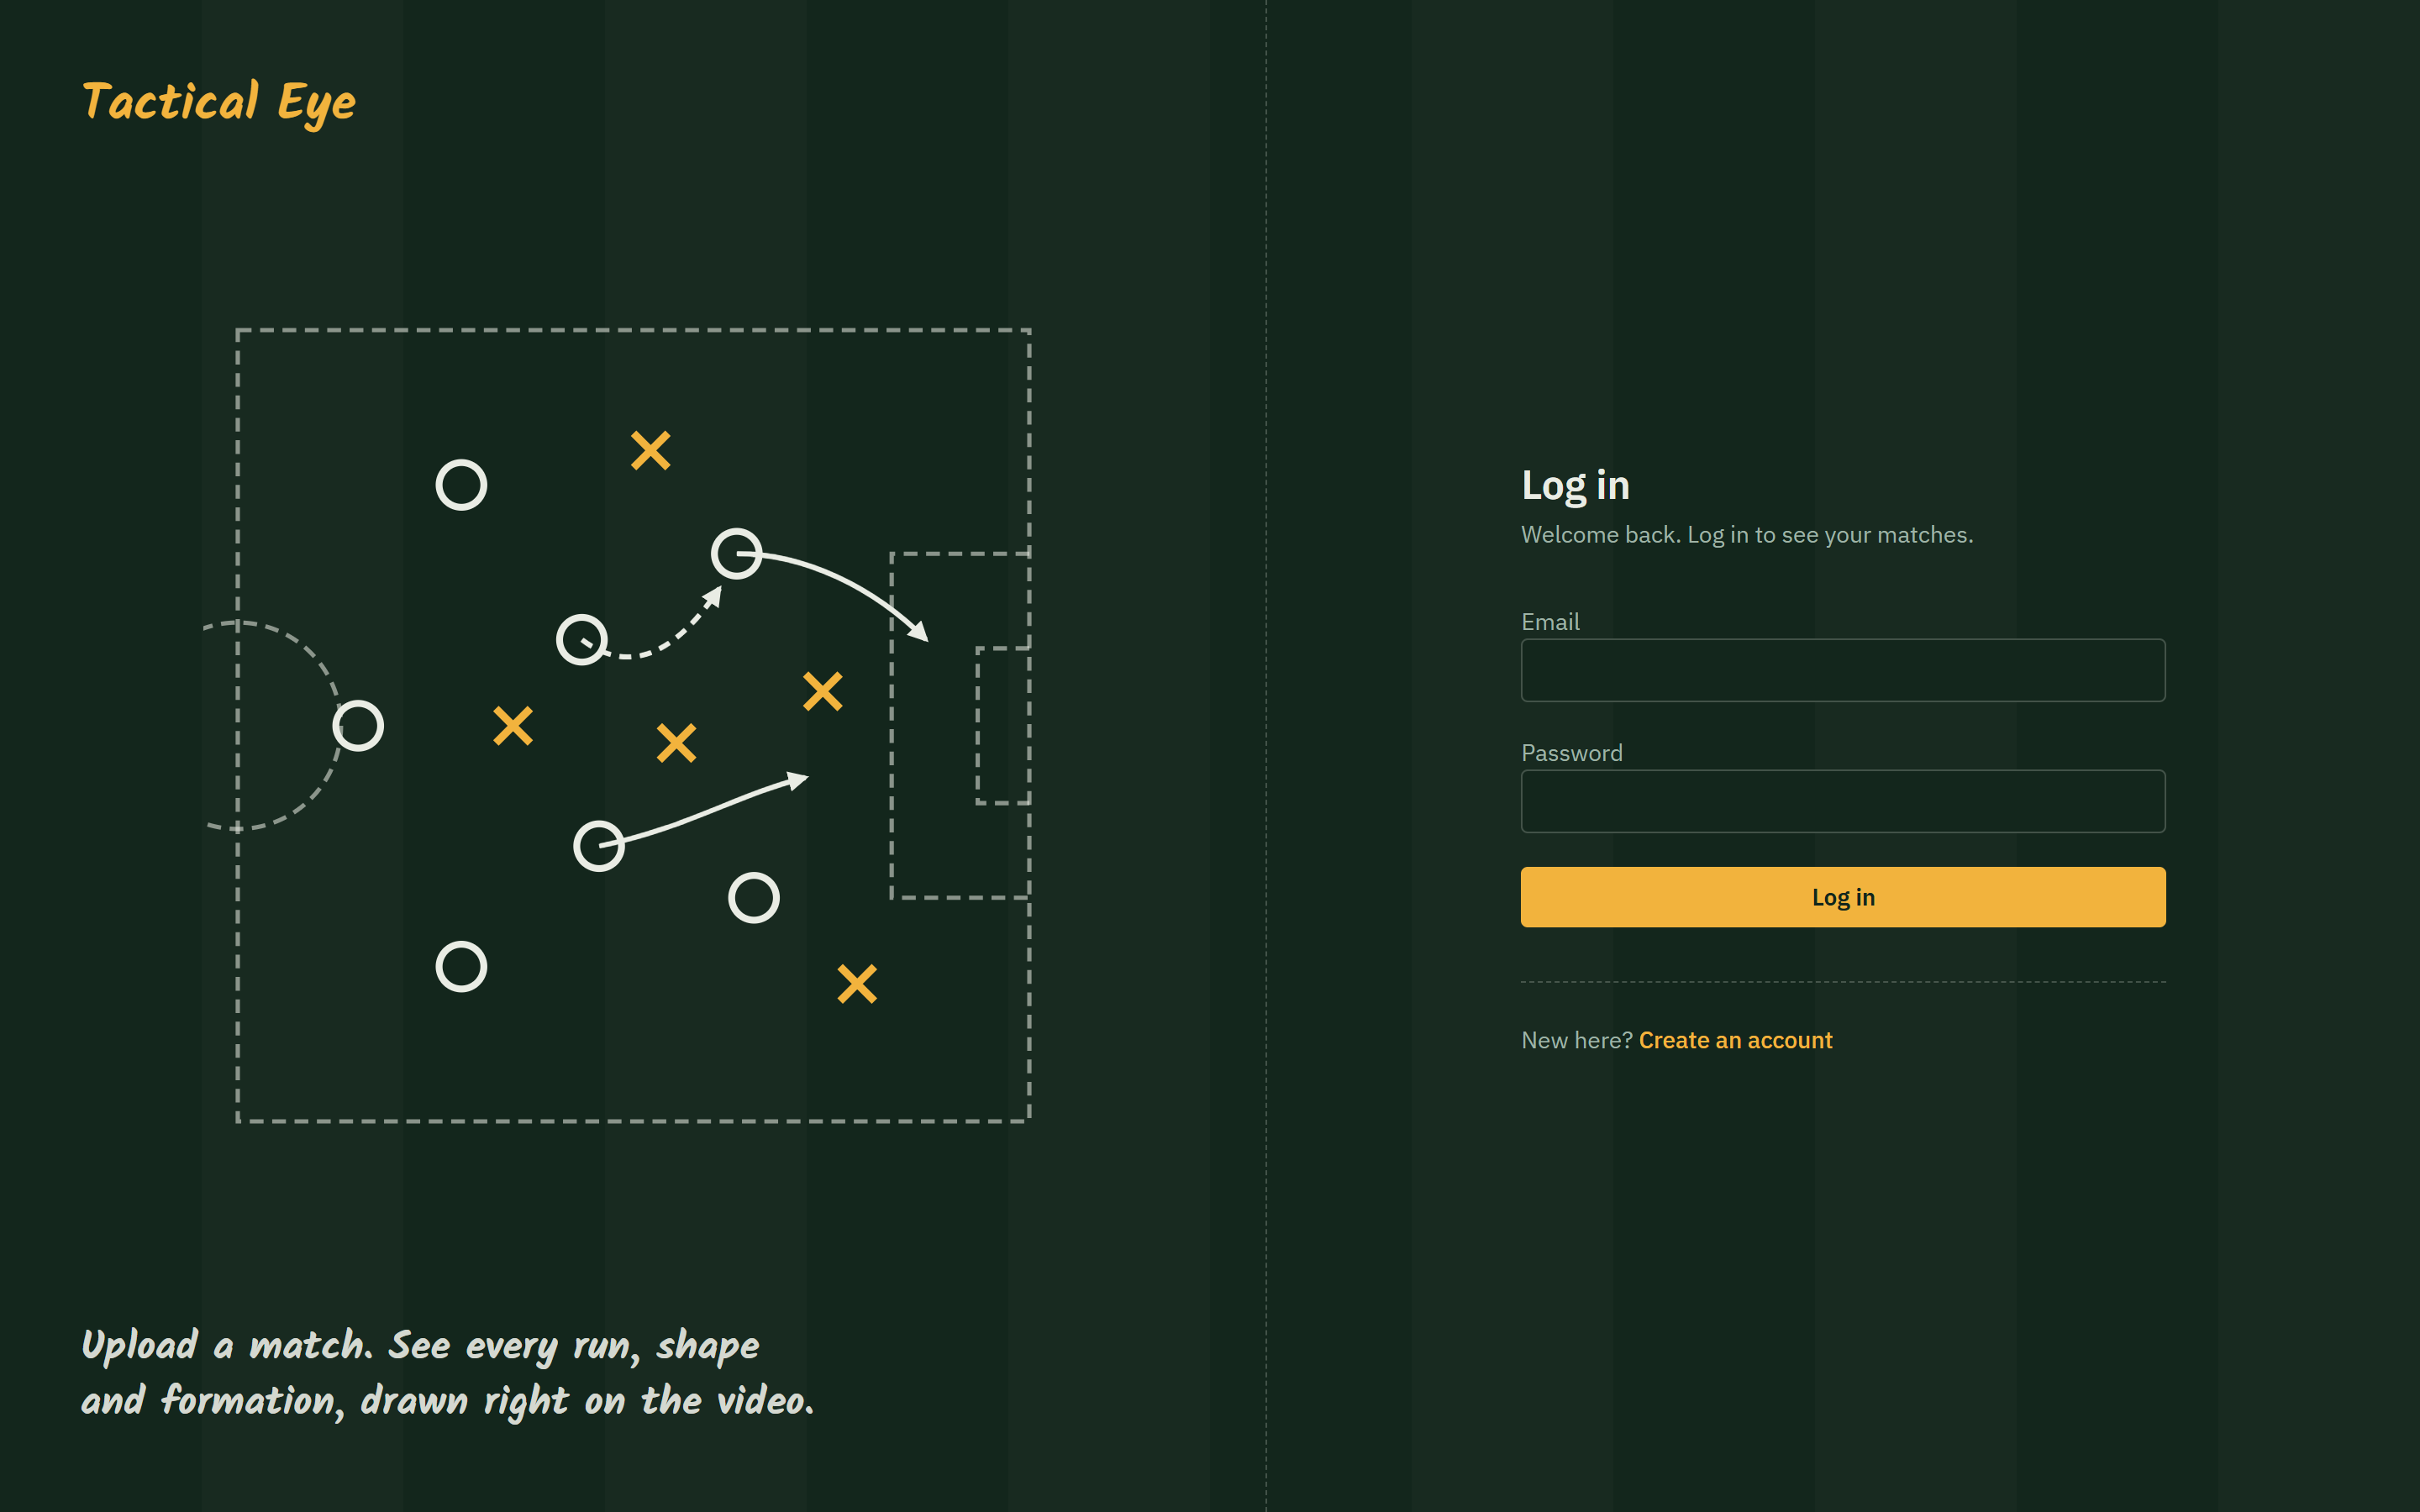
\includegraphics[width=\textwidth]{01_login}
		\caption{Log in}
		\label{fig:login}
	\end{subfigure}
	\hfill
	\begin{subfigure}{0.49\textwidth}
		\centering
		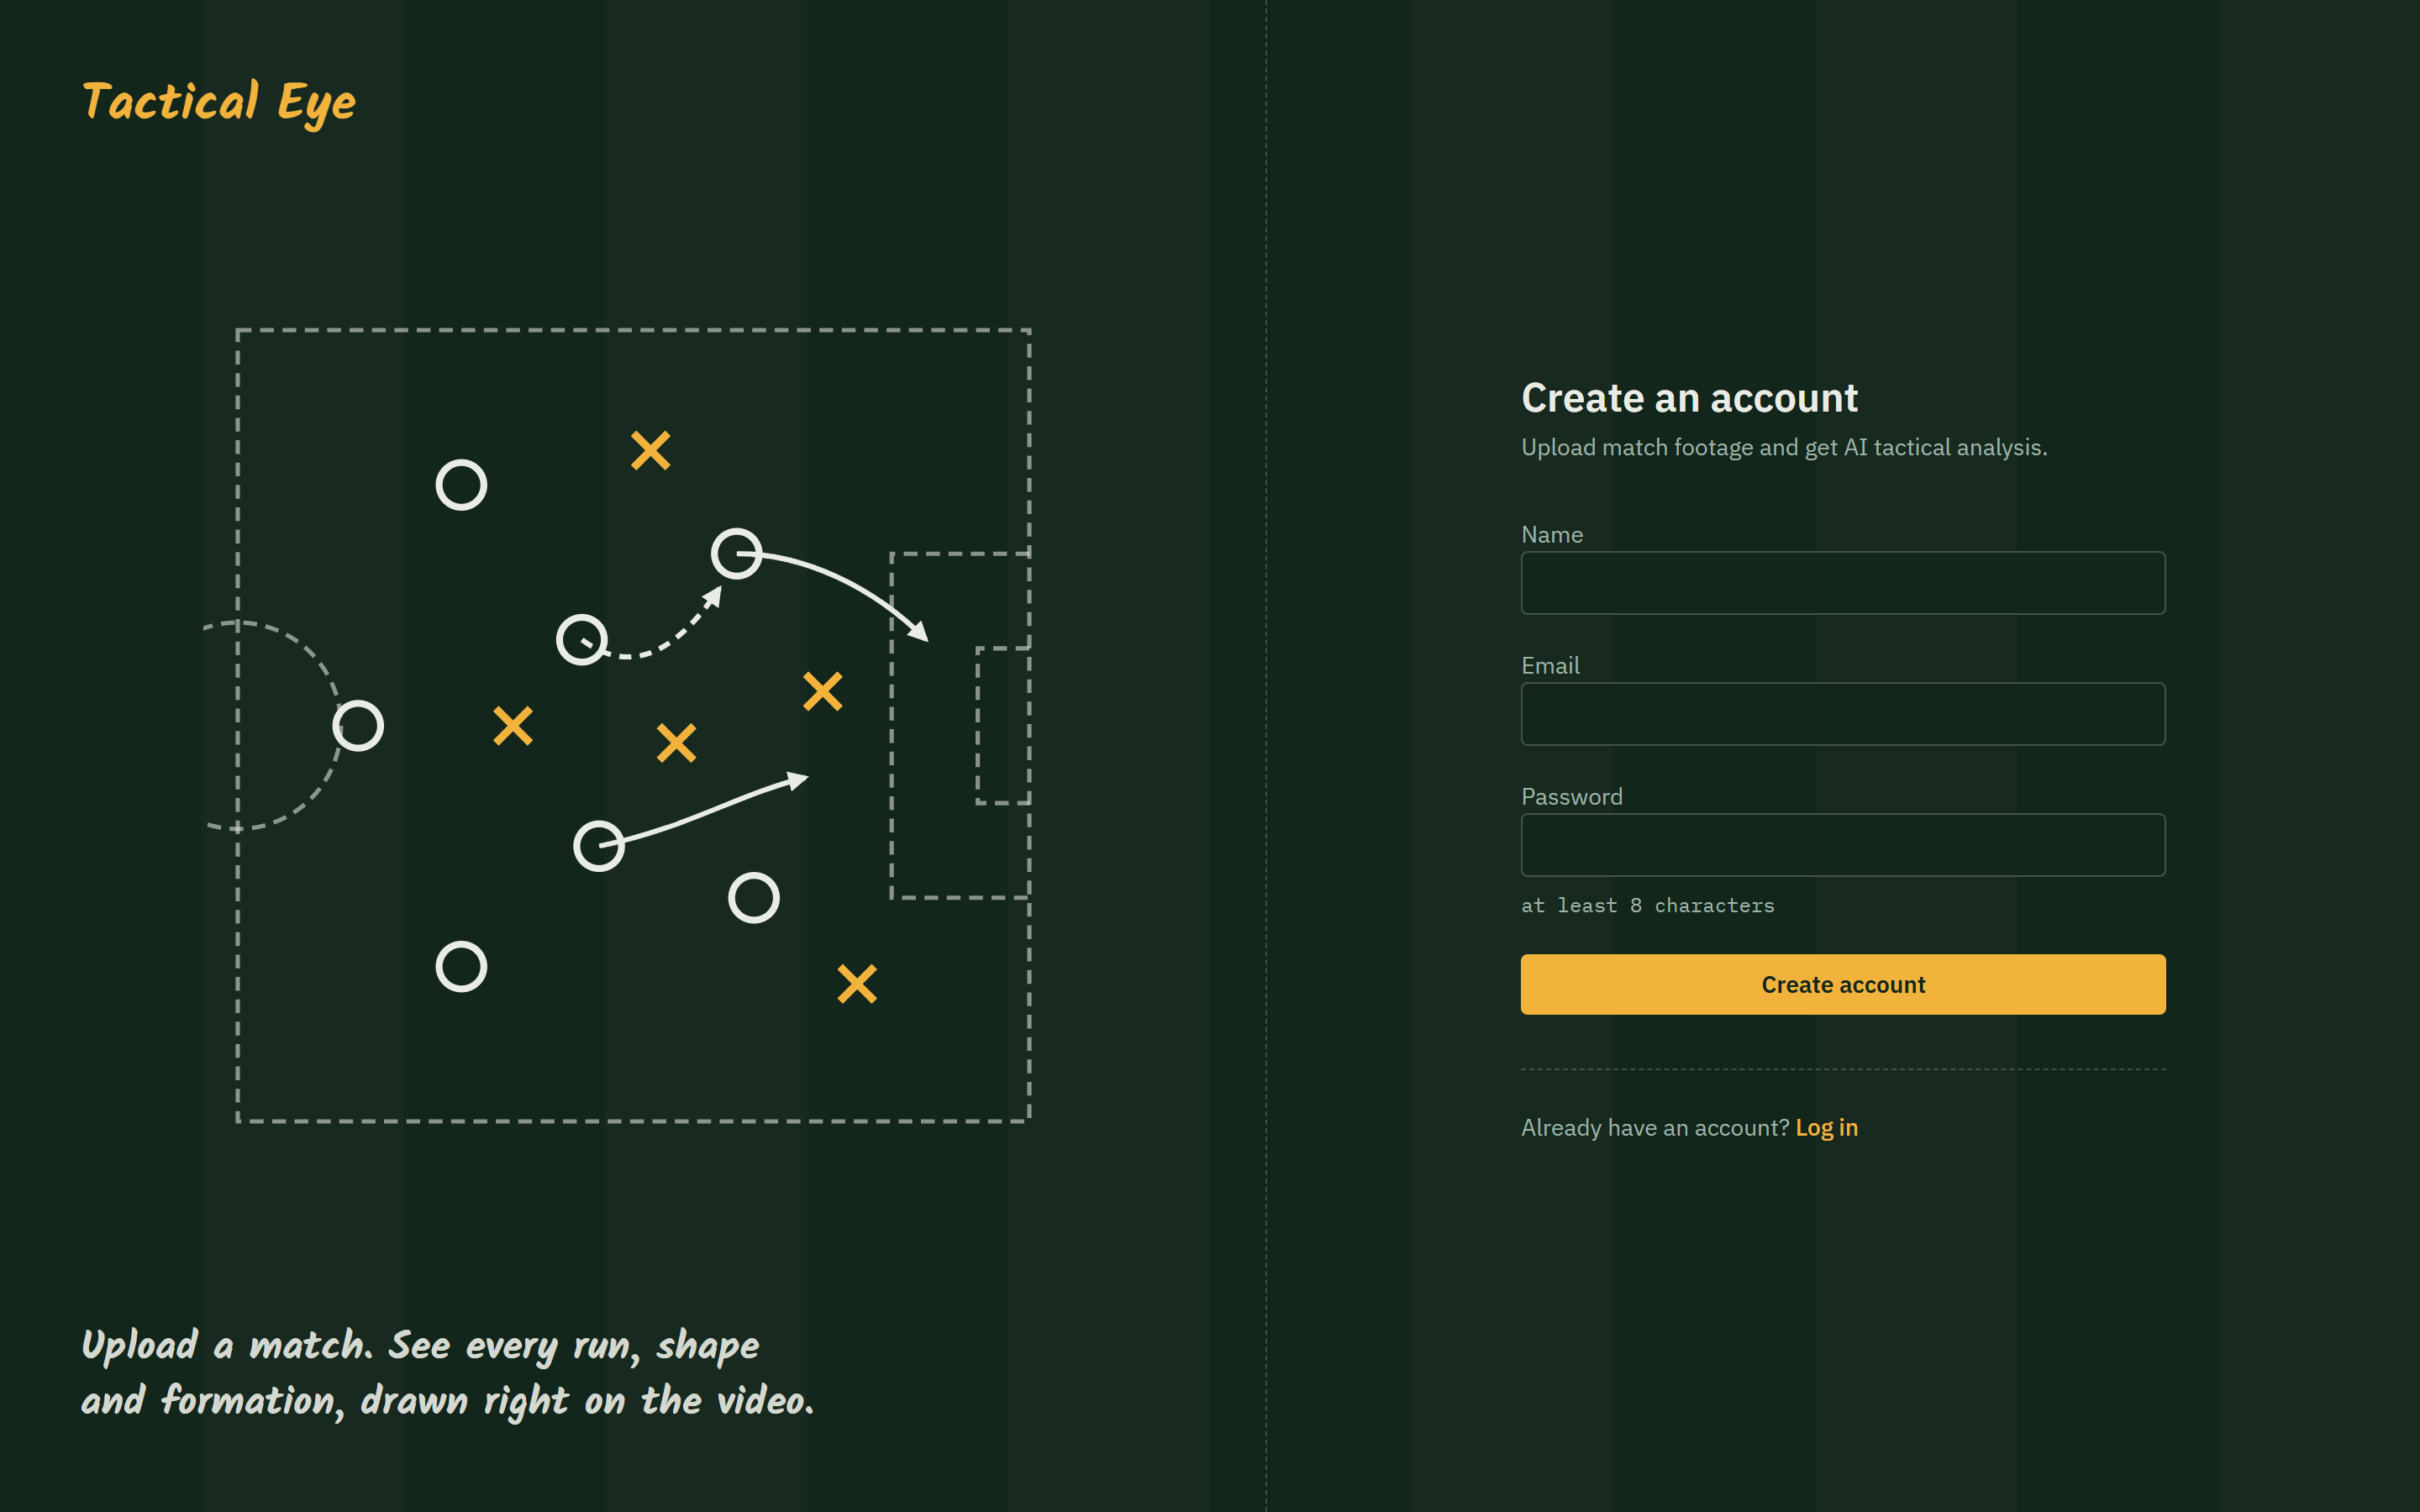
\includegraphics[width=\textwidth]{03_register}
		\caption{Create an account}
		\label{fig:register}
	\end{subfigure}
	\caption{The log-in and registration pages}
	\label{fig:auth-pages}
\end{figure}

A wrong e-mail address or password shows \emph{Invalid email or password} (\autoref{fig:login-error}). The message deliberately does not reveal whether the e-mail address is registered. A session lasts seven days; after that, or after \emph{Log out}, the user logs in again.

\begin{figure}[H]
	\centering
	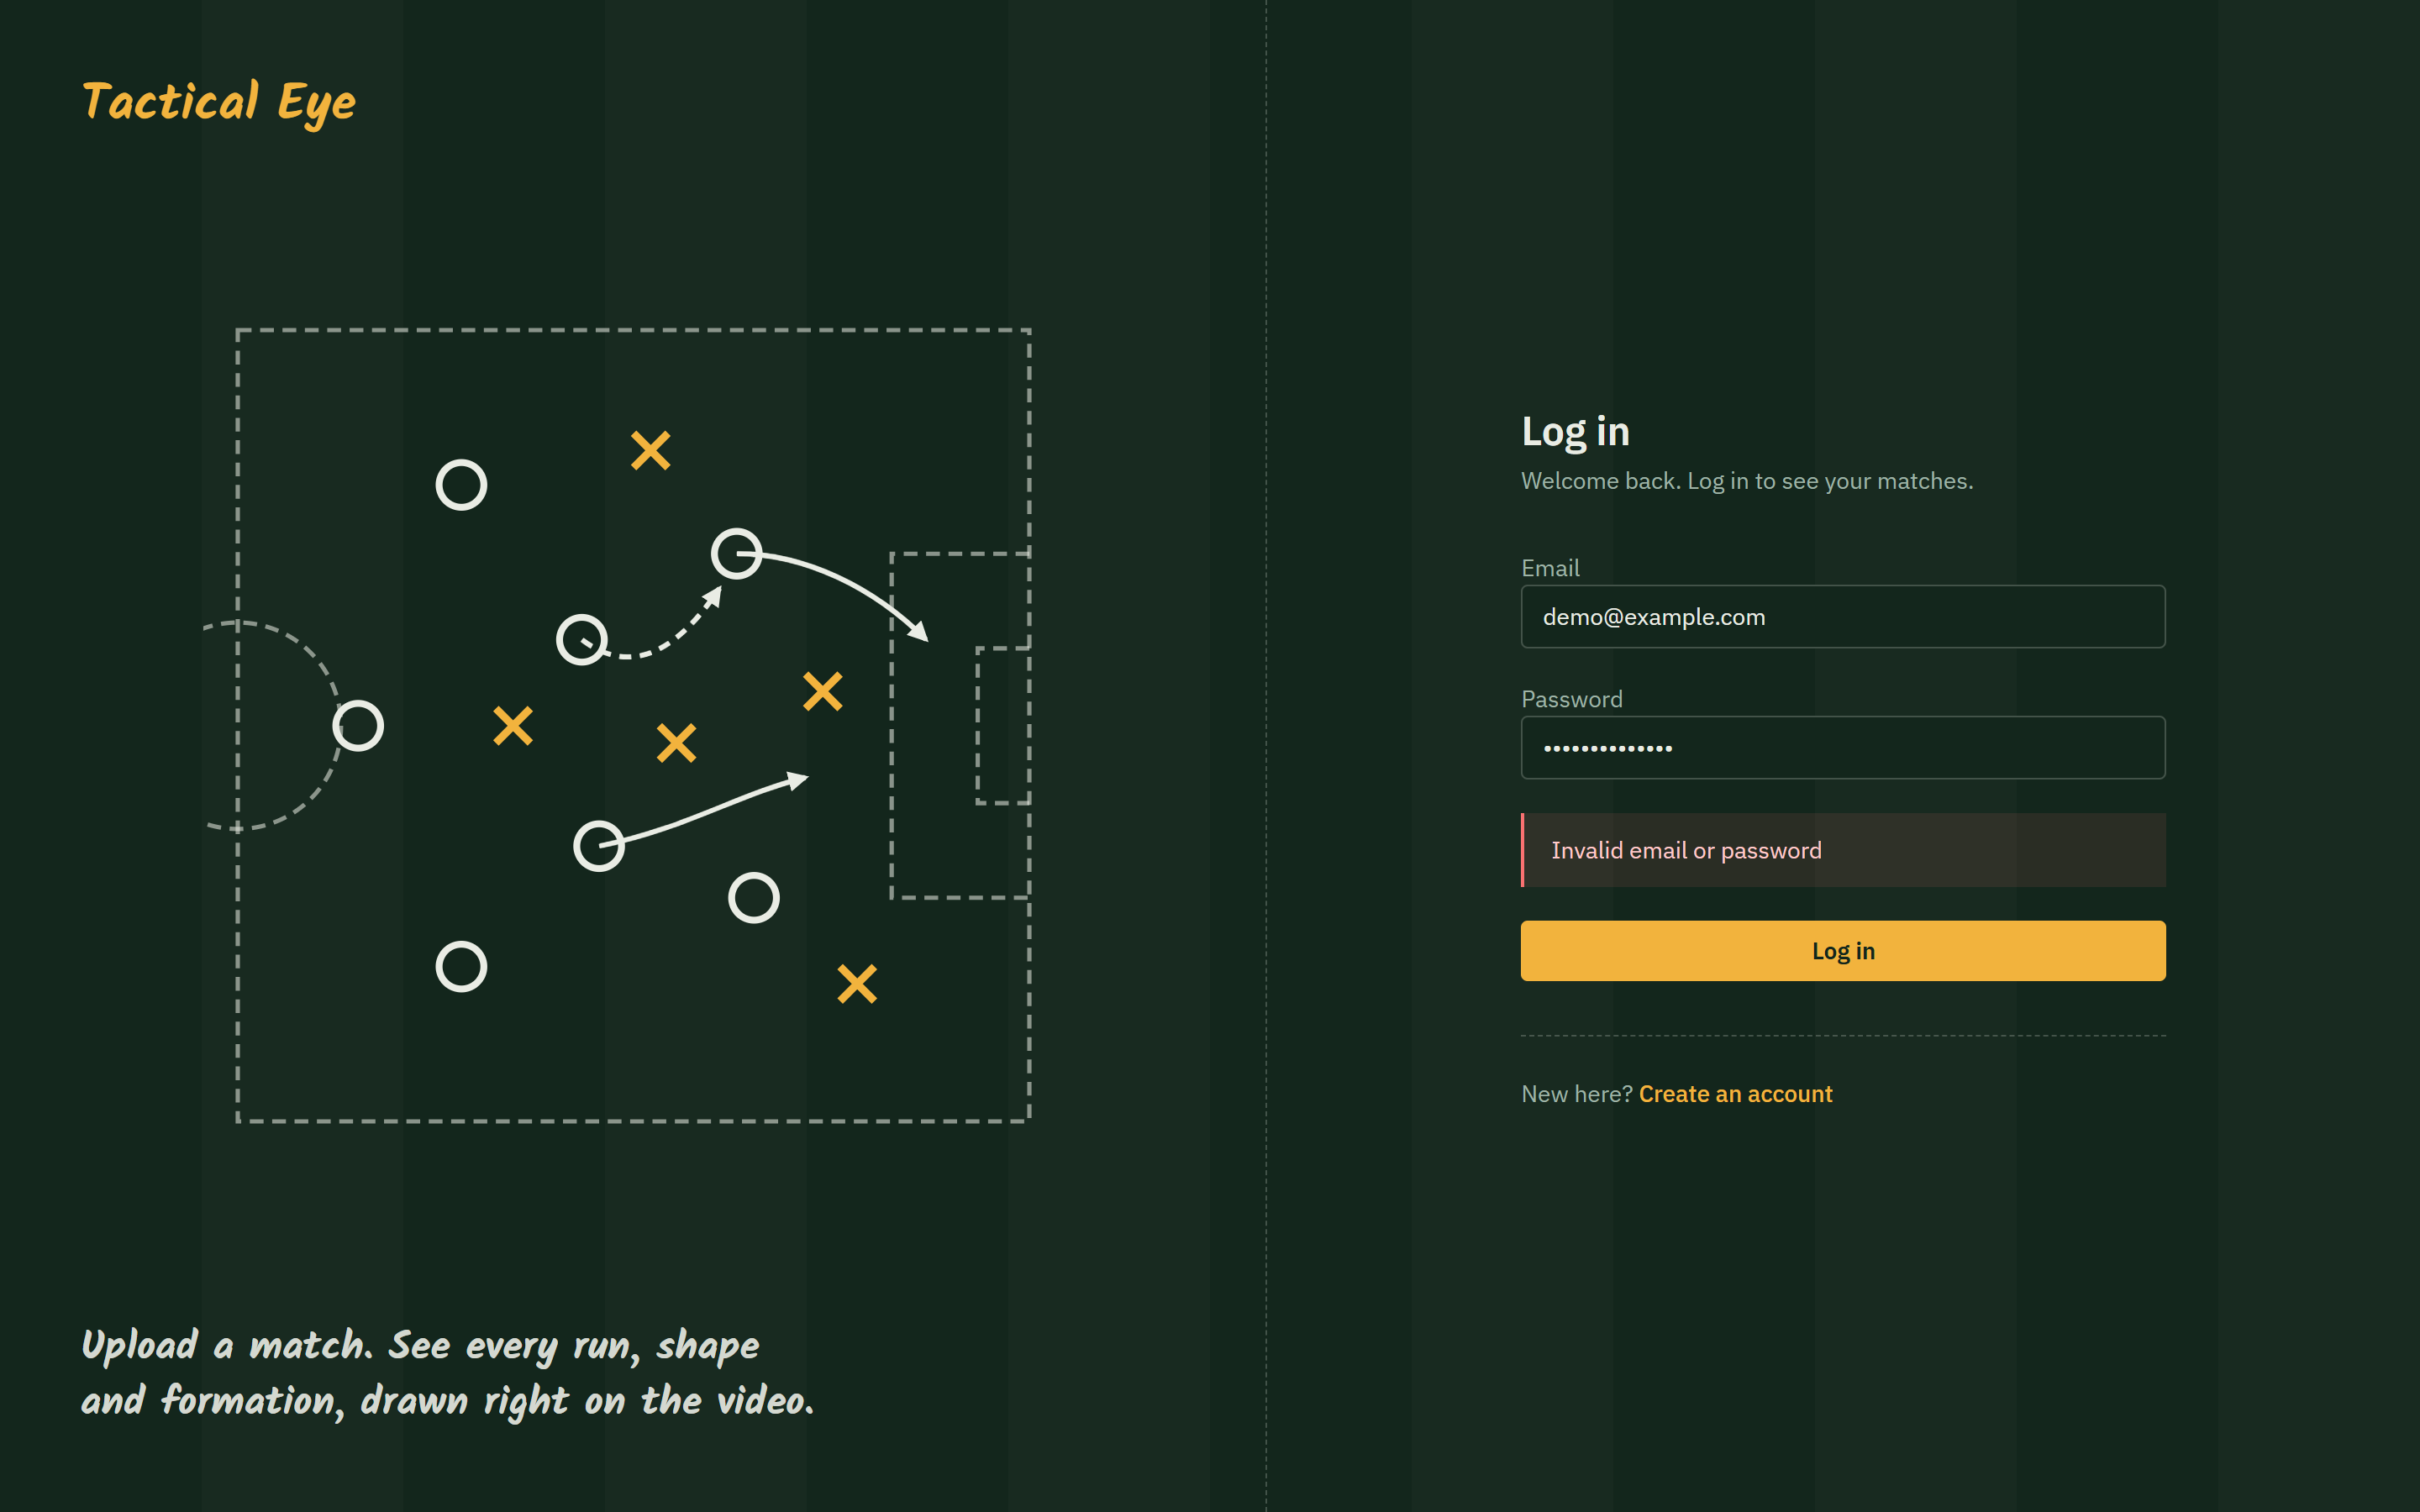
\includegraphics[width=0.75\textwidth]{02_login_error}
	\caption{A failed log-in attempt}
	\label{fig:login-error}
\end{figure}

\subsection{Navigation}

After logging in, every page has the same slim header: the \emph{Tactical Eye} logo, which leads to the match list, the \emph{Matches} and \emph{Upload} links, the user's name and \emph{Log out}. The dashboard is a single-page application, so moving between pages does not reload the browser window, and the browser's back and forward buttons work as usual.

\section{The match list}

The \emph{Matches} page (\autoref{fig:matches}) lists the user's uploads as rows, newest first. Each row shows the title, the upload date, the file size and the analysis mode, a handwritten status note (\autoref{tab:status}), and for finished matches each team's kit colour and its most frequent formation. \emph{+ Upload a match} opens the upload page; clicking a row opens the match.

\begin{figure}[H]
	\centering
	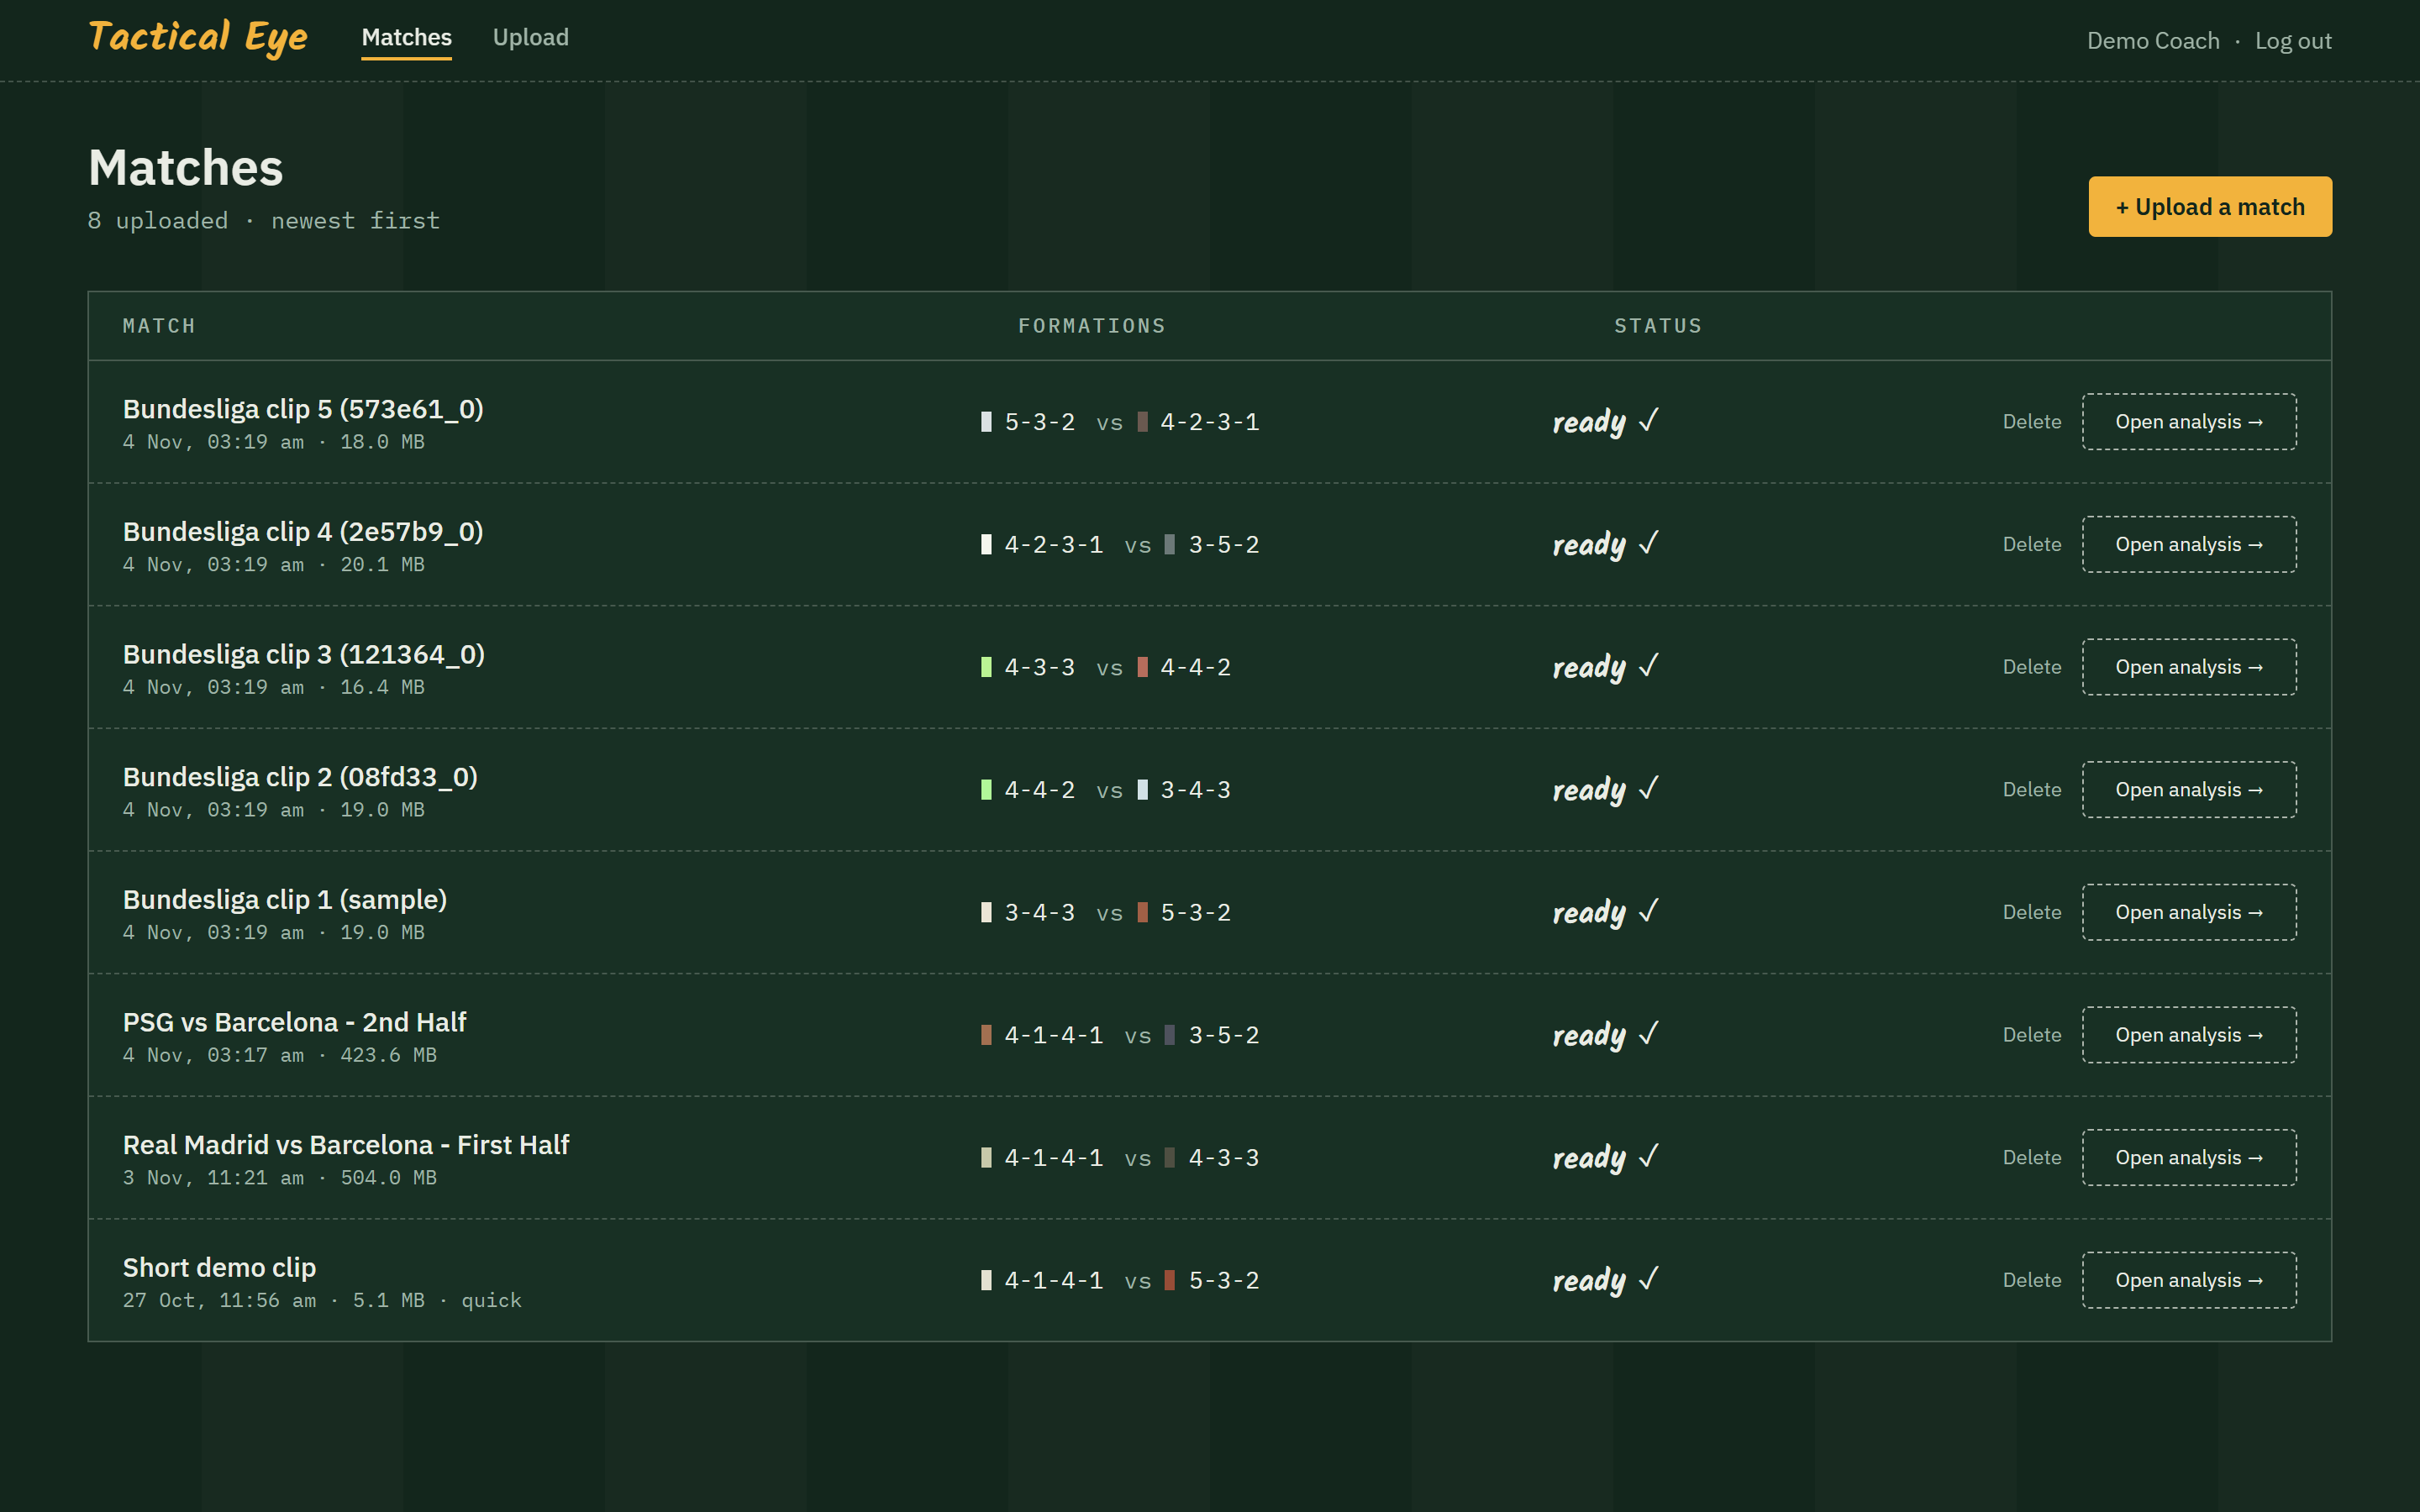
\includegraphics[width=\textwidth]{04_matches}
	\caption{The match list with two analysed halves and the five demo clips}
	\label{fig:matches}
\end{figure}

\begin{table}[H]
	\centering
	\begin{tabular}{|p{0.18\textwidth}|p{0.74\textwidth}|}
		\hline
		\textbf{Status} & \textbf{Meaning} \\
		\hline
		queued\dots & The video is stored and waits for a free worker. Videos are analysed one at a time, in upload order. \\
		\hline
		analysing\dots & A worker is processing the video; the row shows a progress bar and the current step. \\
		\hline
		ready \checkmark & The analysis is finished and can be opened. \\
		\hline
		failed $\times$ & The analysis could not be completed; the row shows the reason (\autoref{sec:messages}). \\
		\hline
		cancelled -- & The user stopped the analysis; it can be started again with \emph{Re-analyse}. \\
		\hline
	\end{tabular}
	\caption{Status notes}
	\label{tab:status}
\end{table}

The list updates itself: progress bars move, statuses change and new matches appear without reloading the page, because the server pushes every change to the browser.

\section{Uploading a match}

The upload page (\autoref{fig:upload-empty}) leads through three numbered steps, with tips for good results on the right.

\begin{enumerate}
	\item \emph{Choose the video}: drag a file onto the dashed area or click it to pick one. MP4, MOV, M4V, MKV, WebM and AVI files are accepted, up to 1\,GB, which is enough for a full half (\autoref{fig:upload-ready}). Any codec and frame rate works; the server converts the video for the browser.
	\item \emph{Give it a name}: the title is filled in from the file name and can be up to 120 characters long.
	\item \emph{Pick the analysis mode} (\autoref{tab:modes}).
\end{enumerate}

Then \emph{Upload and analyse} sends the file with a progress bar. When the upload completes, the dashboard opens the new match's page.

\begin{figure}[H]
	\centering
	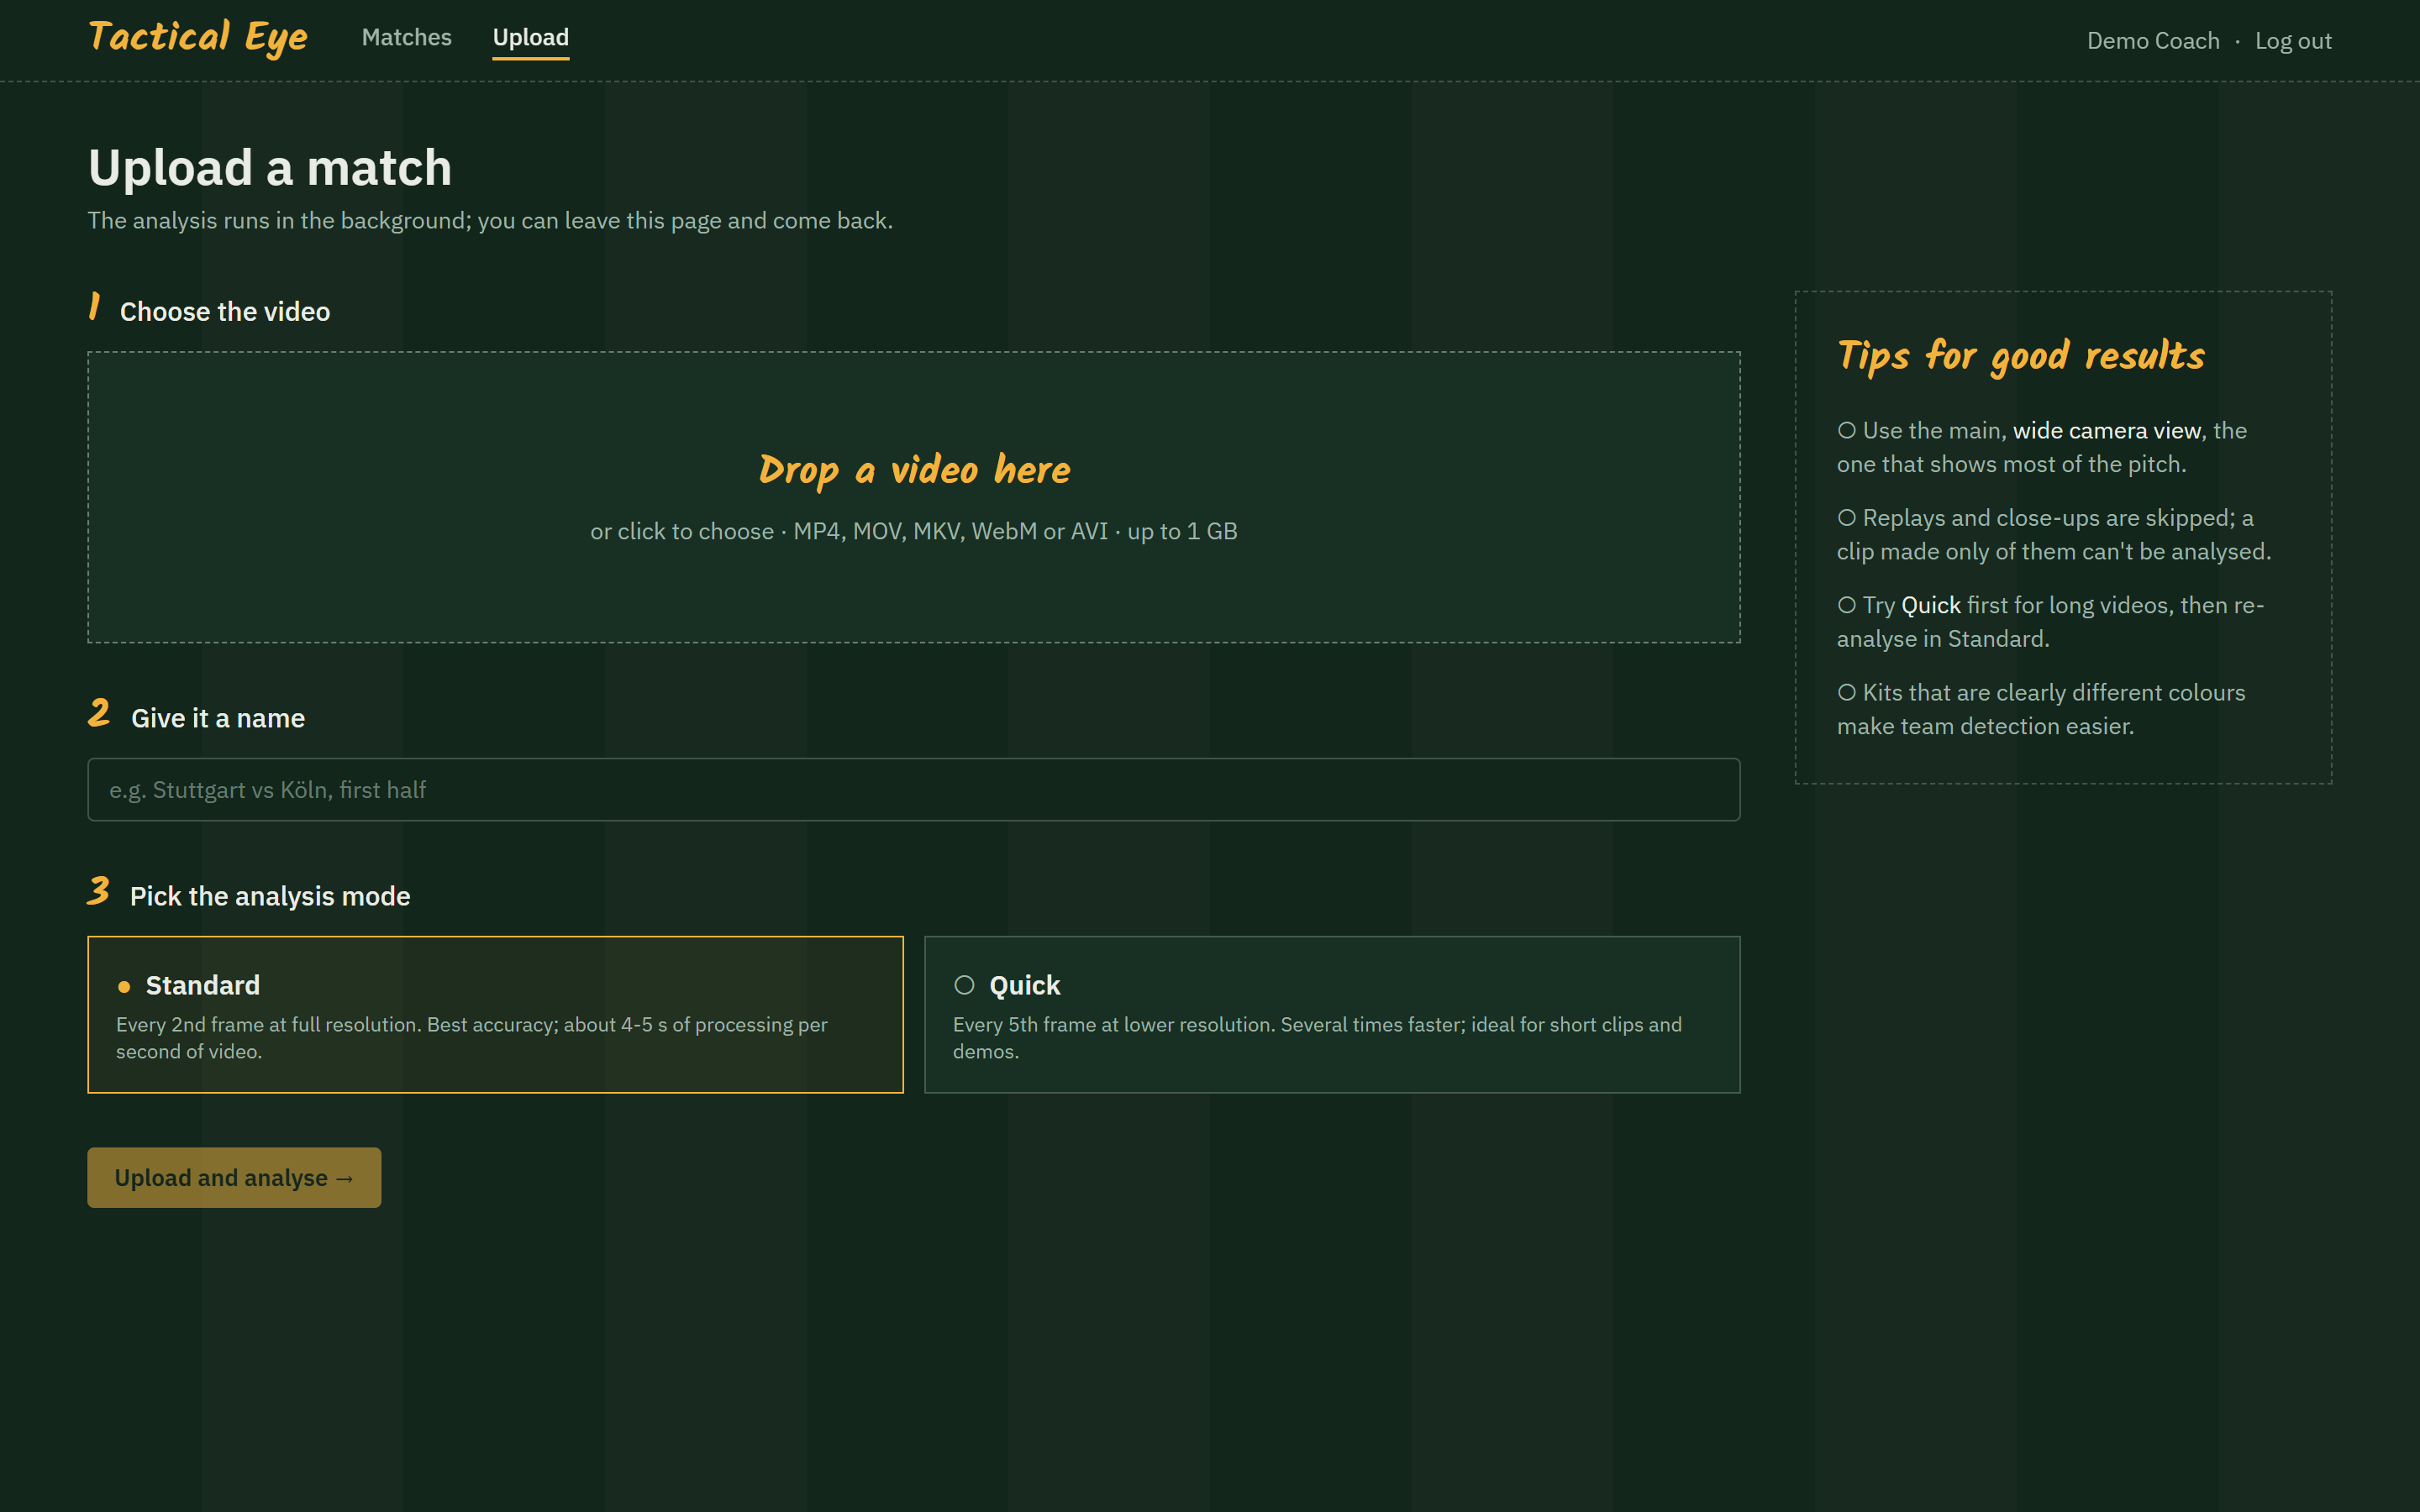
\includegraphics[width=\textwidth]{05_upload_empty}
	\caption{The upload page before a file is chosen}
	\label{fig:upload-empty}
\end{figure}

\begin{figure}[H]
	\centering
	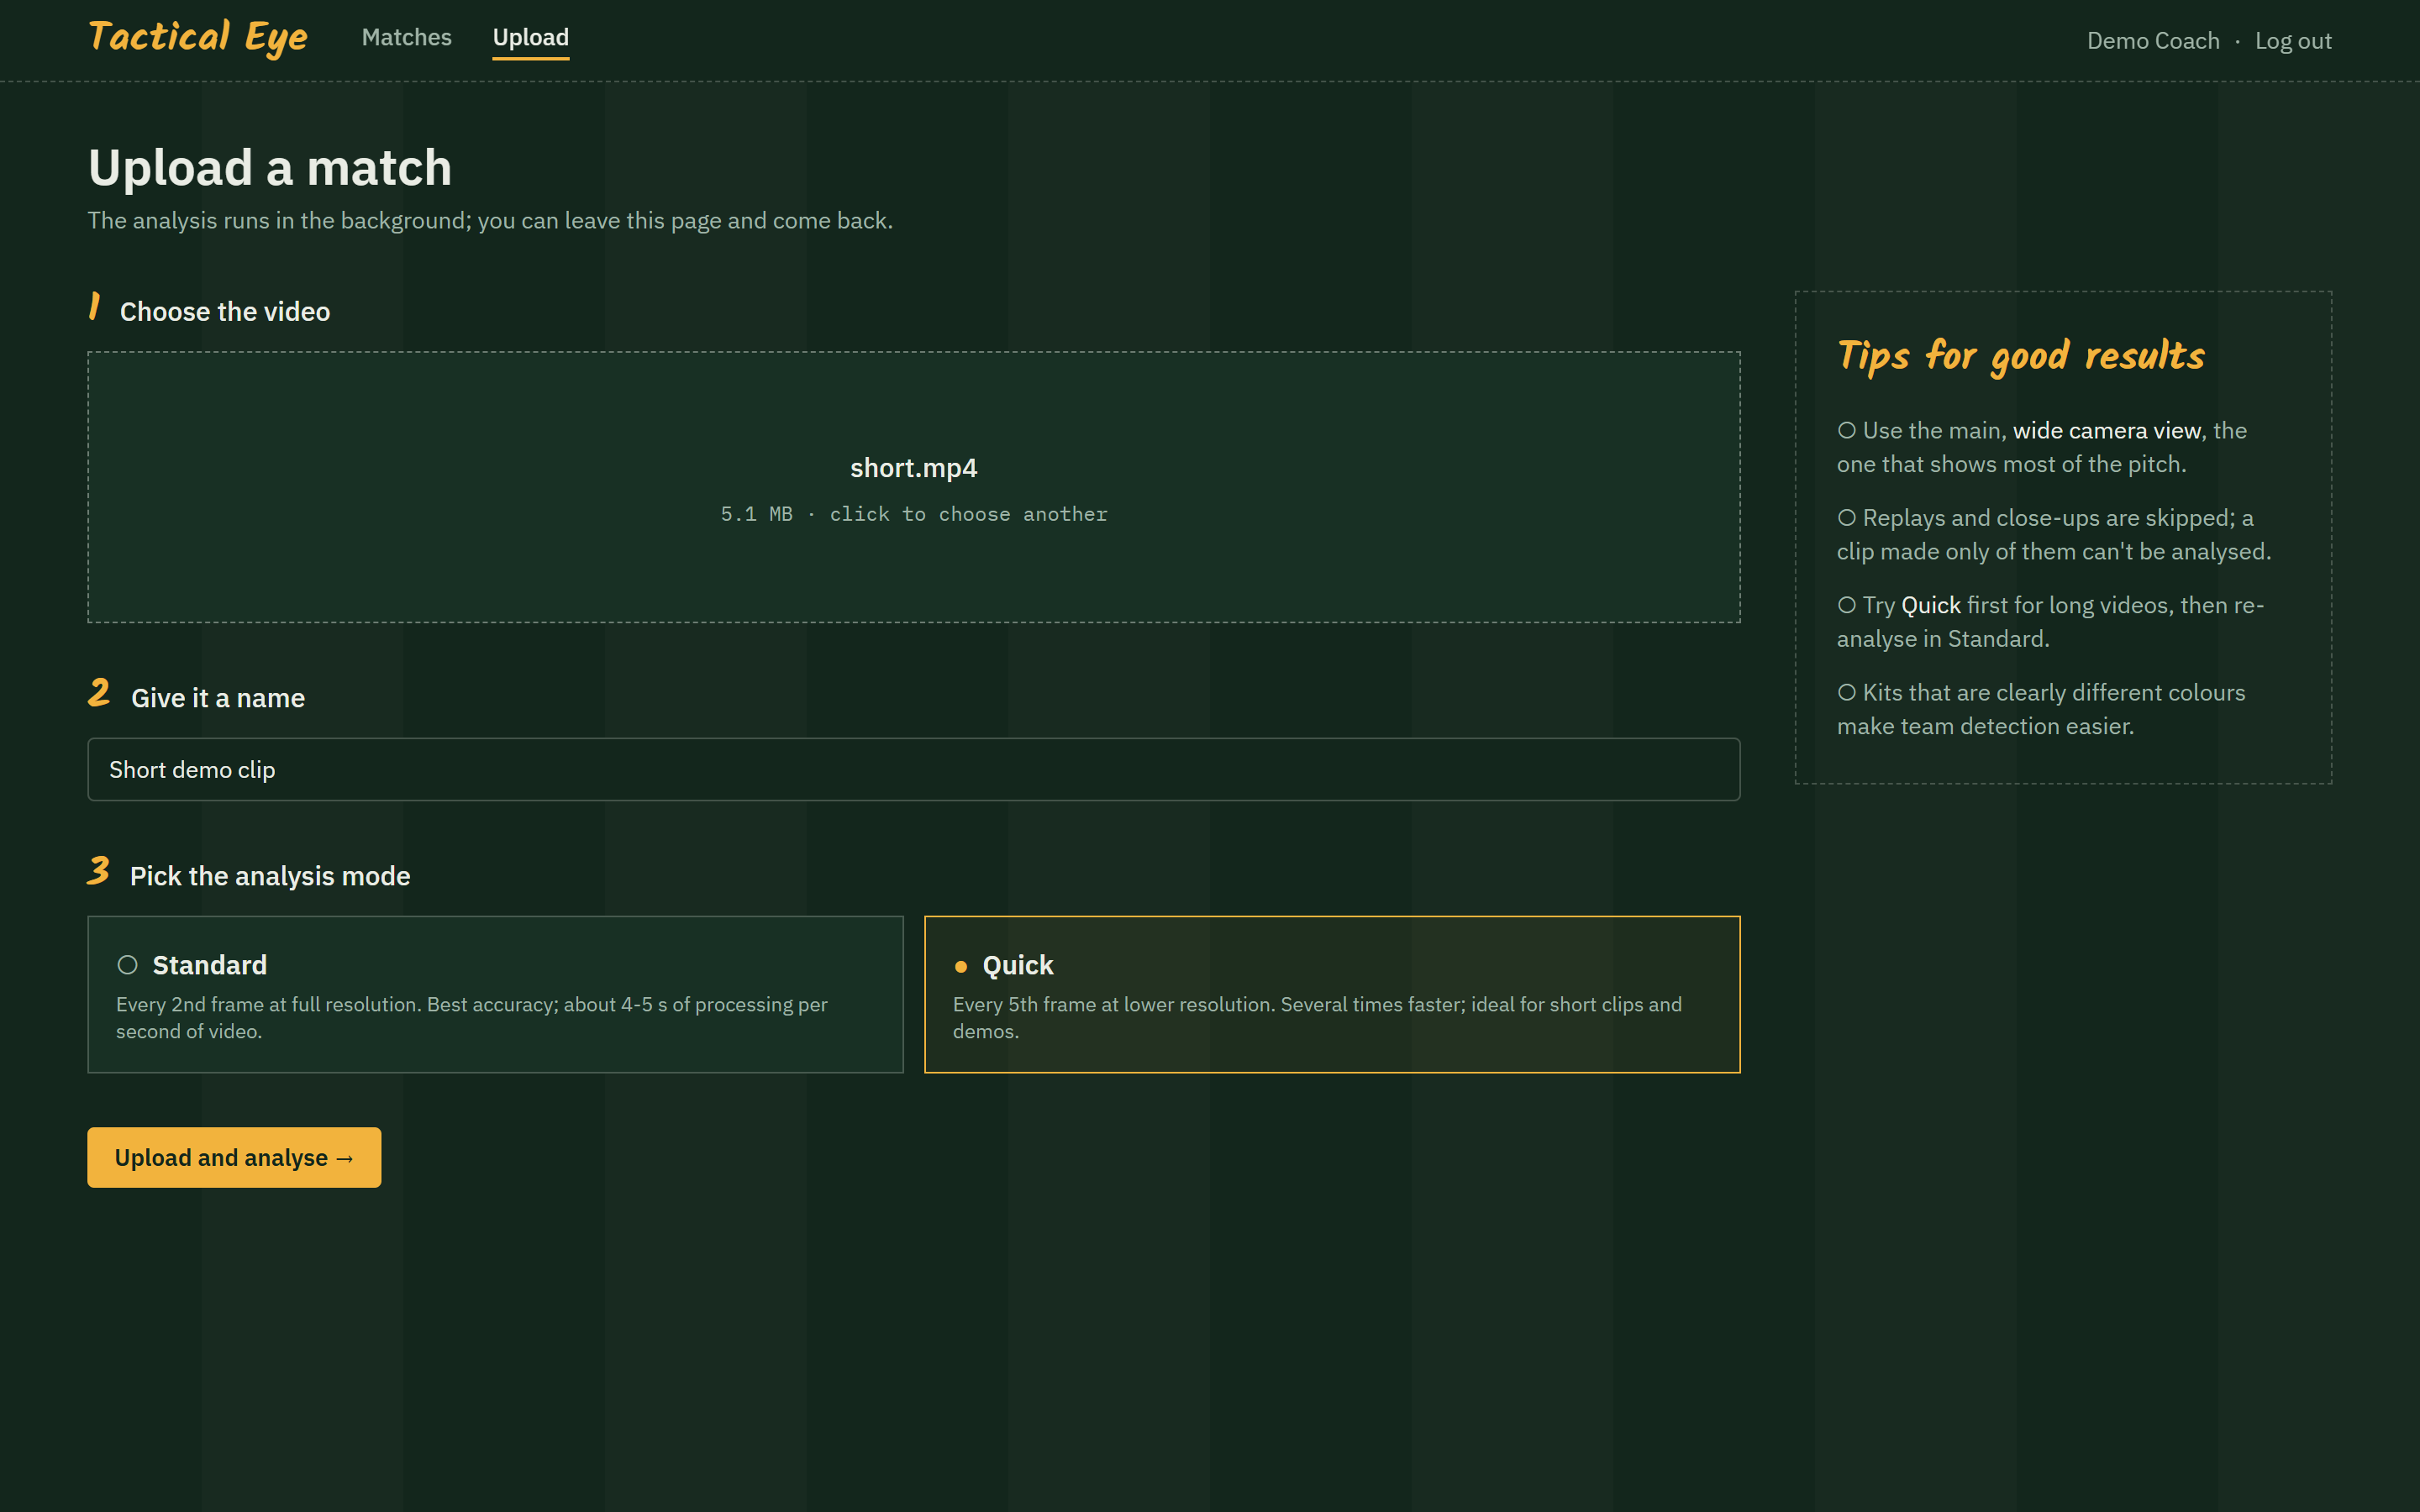
\includegraphics[width=\textwidth]{07_upload_ready}
	\caption{A file is chosen, the title is filled in and Quick mode is selected}
	\label{fig:upload-ready}
\end{figure}

\begin{table}[H]
	\centering
	\begin{tabular}{|p{0.13\textwidth}|p{0.38\textwidth}|p{0.40\textwidth}|}
		\hline
		\textbf{Mode} & \textbf{What it does} & \textbf{When to use it} \\
		\hline
		Standard & Analyses 12.5 frames per second of video (every 2nd frame at 25\,fps, every 4th at 50\,fps) at 1280-pixel detection resolution. & Best accuracy; the default, and the mode used for full halves on a GPU. \\
		\hline
		Quick & Analyses 5 frames per second at 960 pixels. & Several times faster, for short clips, previews and live demonstrations. The ball is found less often. \\
		\hline
	\end{tabular}
	\caption{Analysis modes}
	\label{tab:modes}
\end{table}

Footage from the main, wide camera gives the best results. Close-ups, replays and crowd shots contain no usable view of the pitch; the analysis skips them, but a video made mostly of them cannot be analysed (\autoref{sec:messages}).

Every upload is checked on the server. A file that is not really a video, for example a text file renamed to \texttt{.\allowbreak{}mp4}, is rejected with \emph{The file is not a valid video} and nothing is stored (\autoref{fig:upload-invalid}).

\begin{figure}[H]
	\centering
	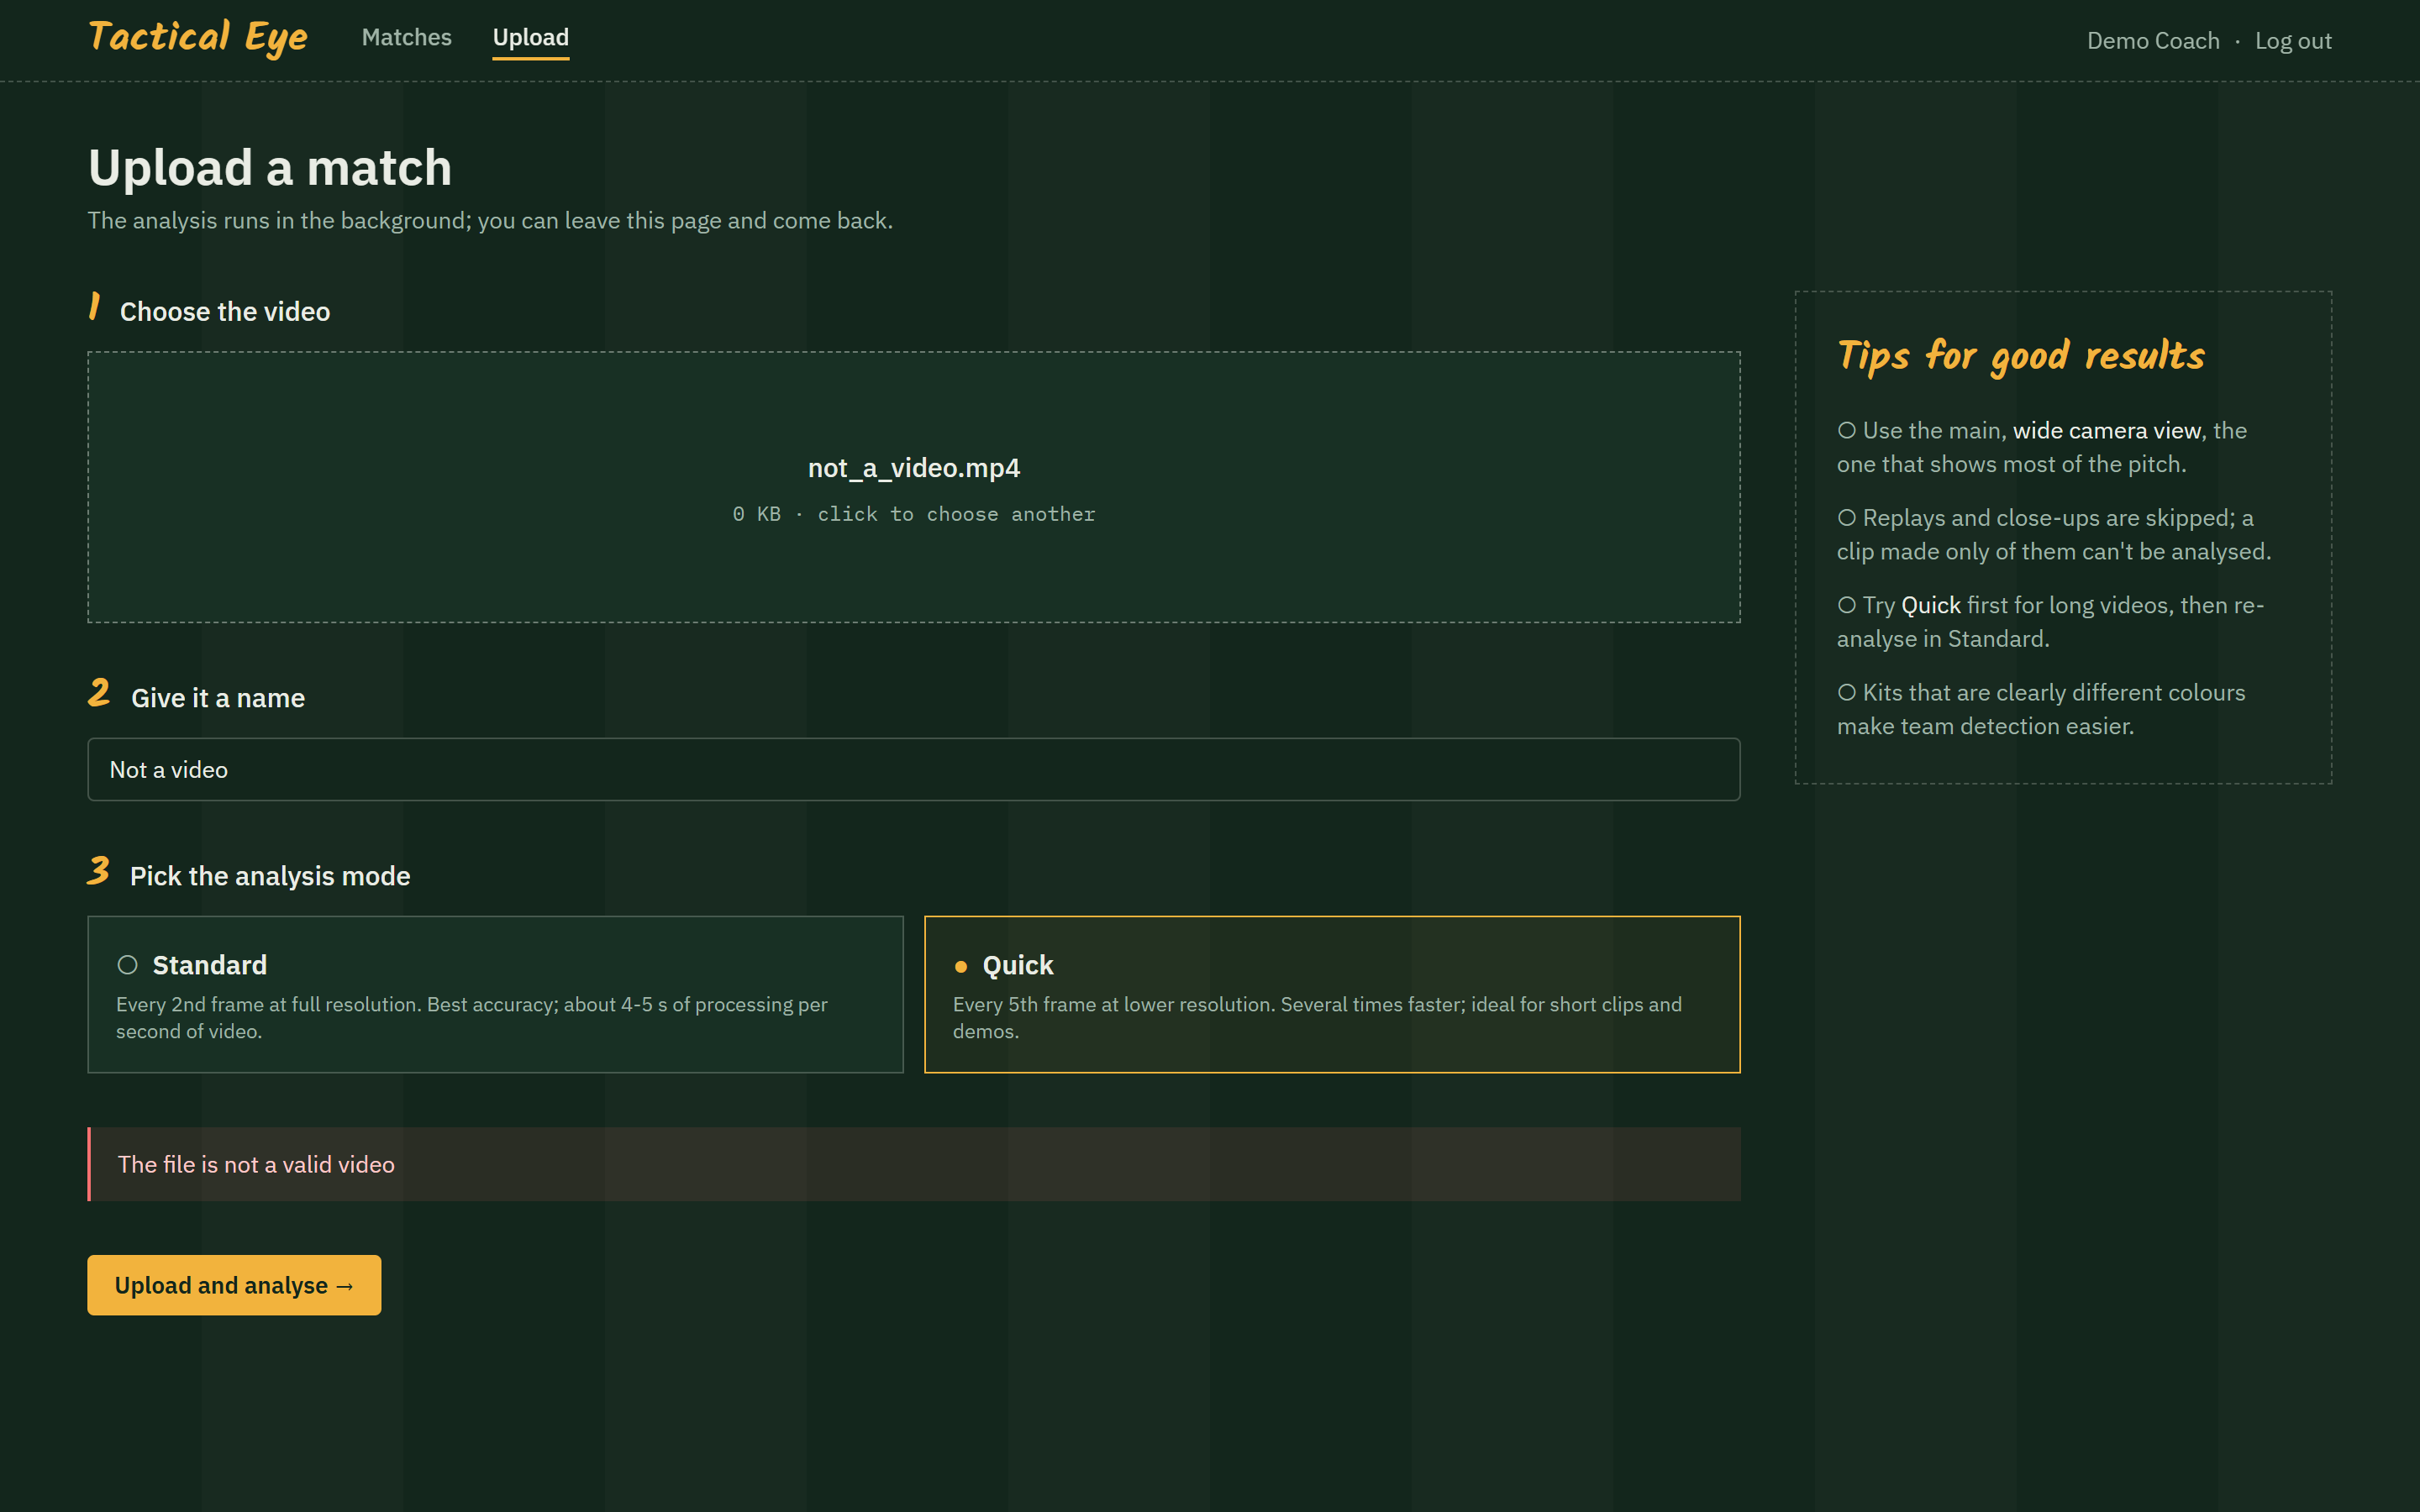
\includegraphics[width=\textwidth]{06_upload_invalid_file}
	\caption{A file that is not a video is rejected}
	\label{fig:upload-invalid}
\end{figure}

\section{Following and cancelling the analysis}

While a video is being analysed, its page shows a progress bar with the current step (\autoref{fig:in-progress}). The page updates live; the user can leave it, close the browser or upload more matches, and the analysis continues on the server. The match list shows the same progress in the match's row (\autoref{fig:list-progress}). \autoref{tab:steps} lists the steps.

\begin{figure}[H]
	\centering
	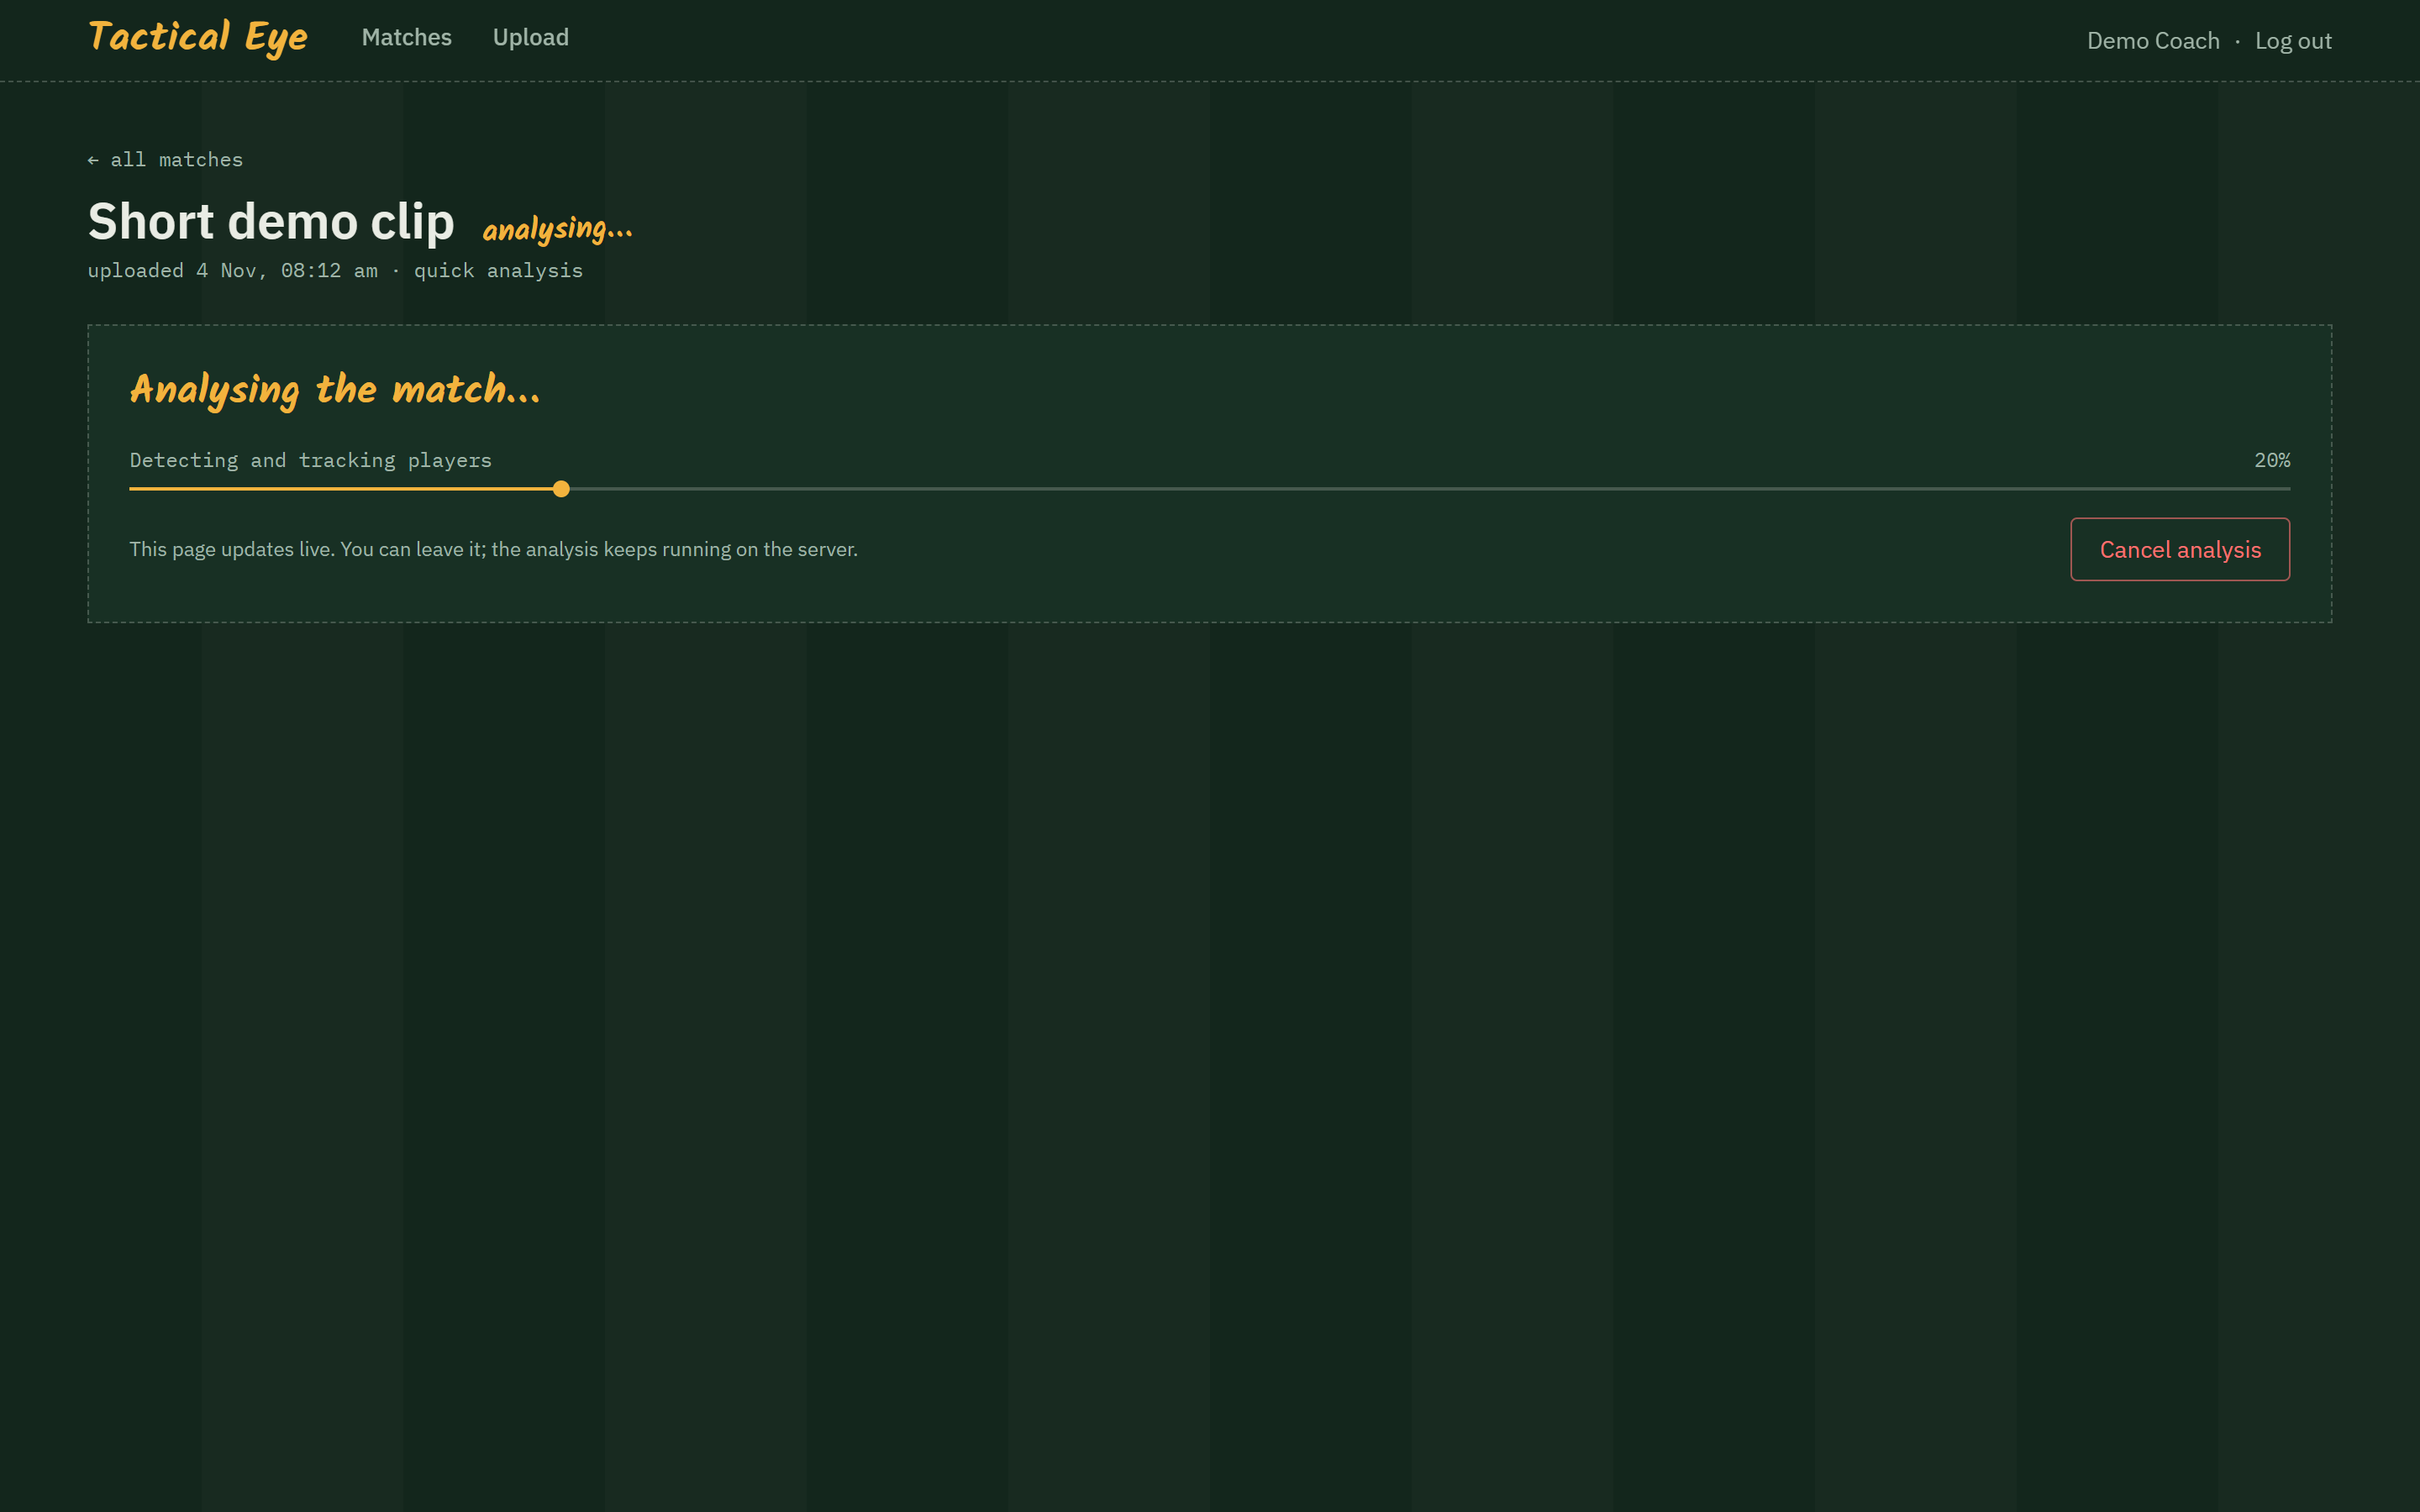
\includegraphics[width=\textwidth]{08_match_in_progress}
	\caption{An analysis in progress, with the \emph{Cancel analysis} button}
	\label{fig:in-progress}
\end{figure}

\begin{figure}[H]
	\centering
	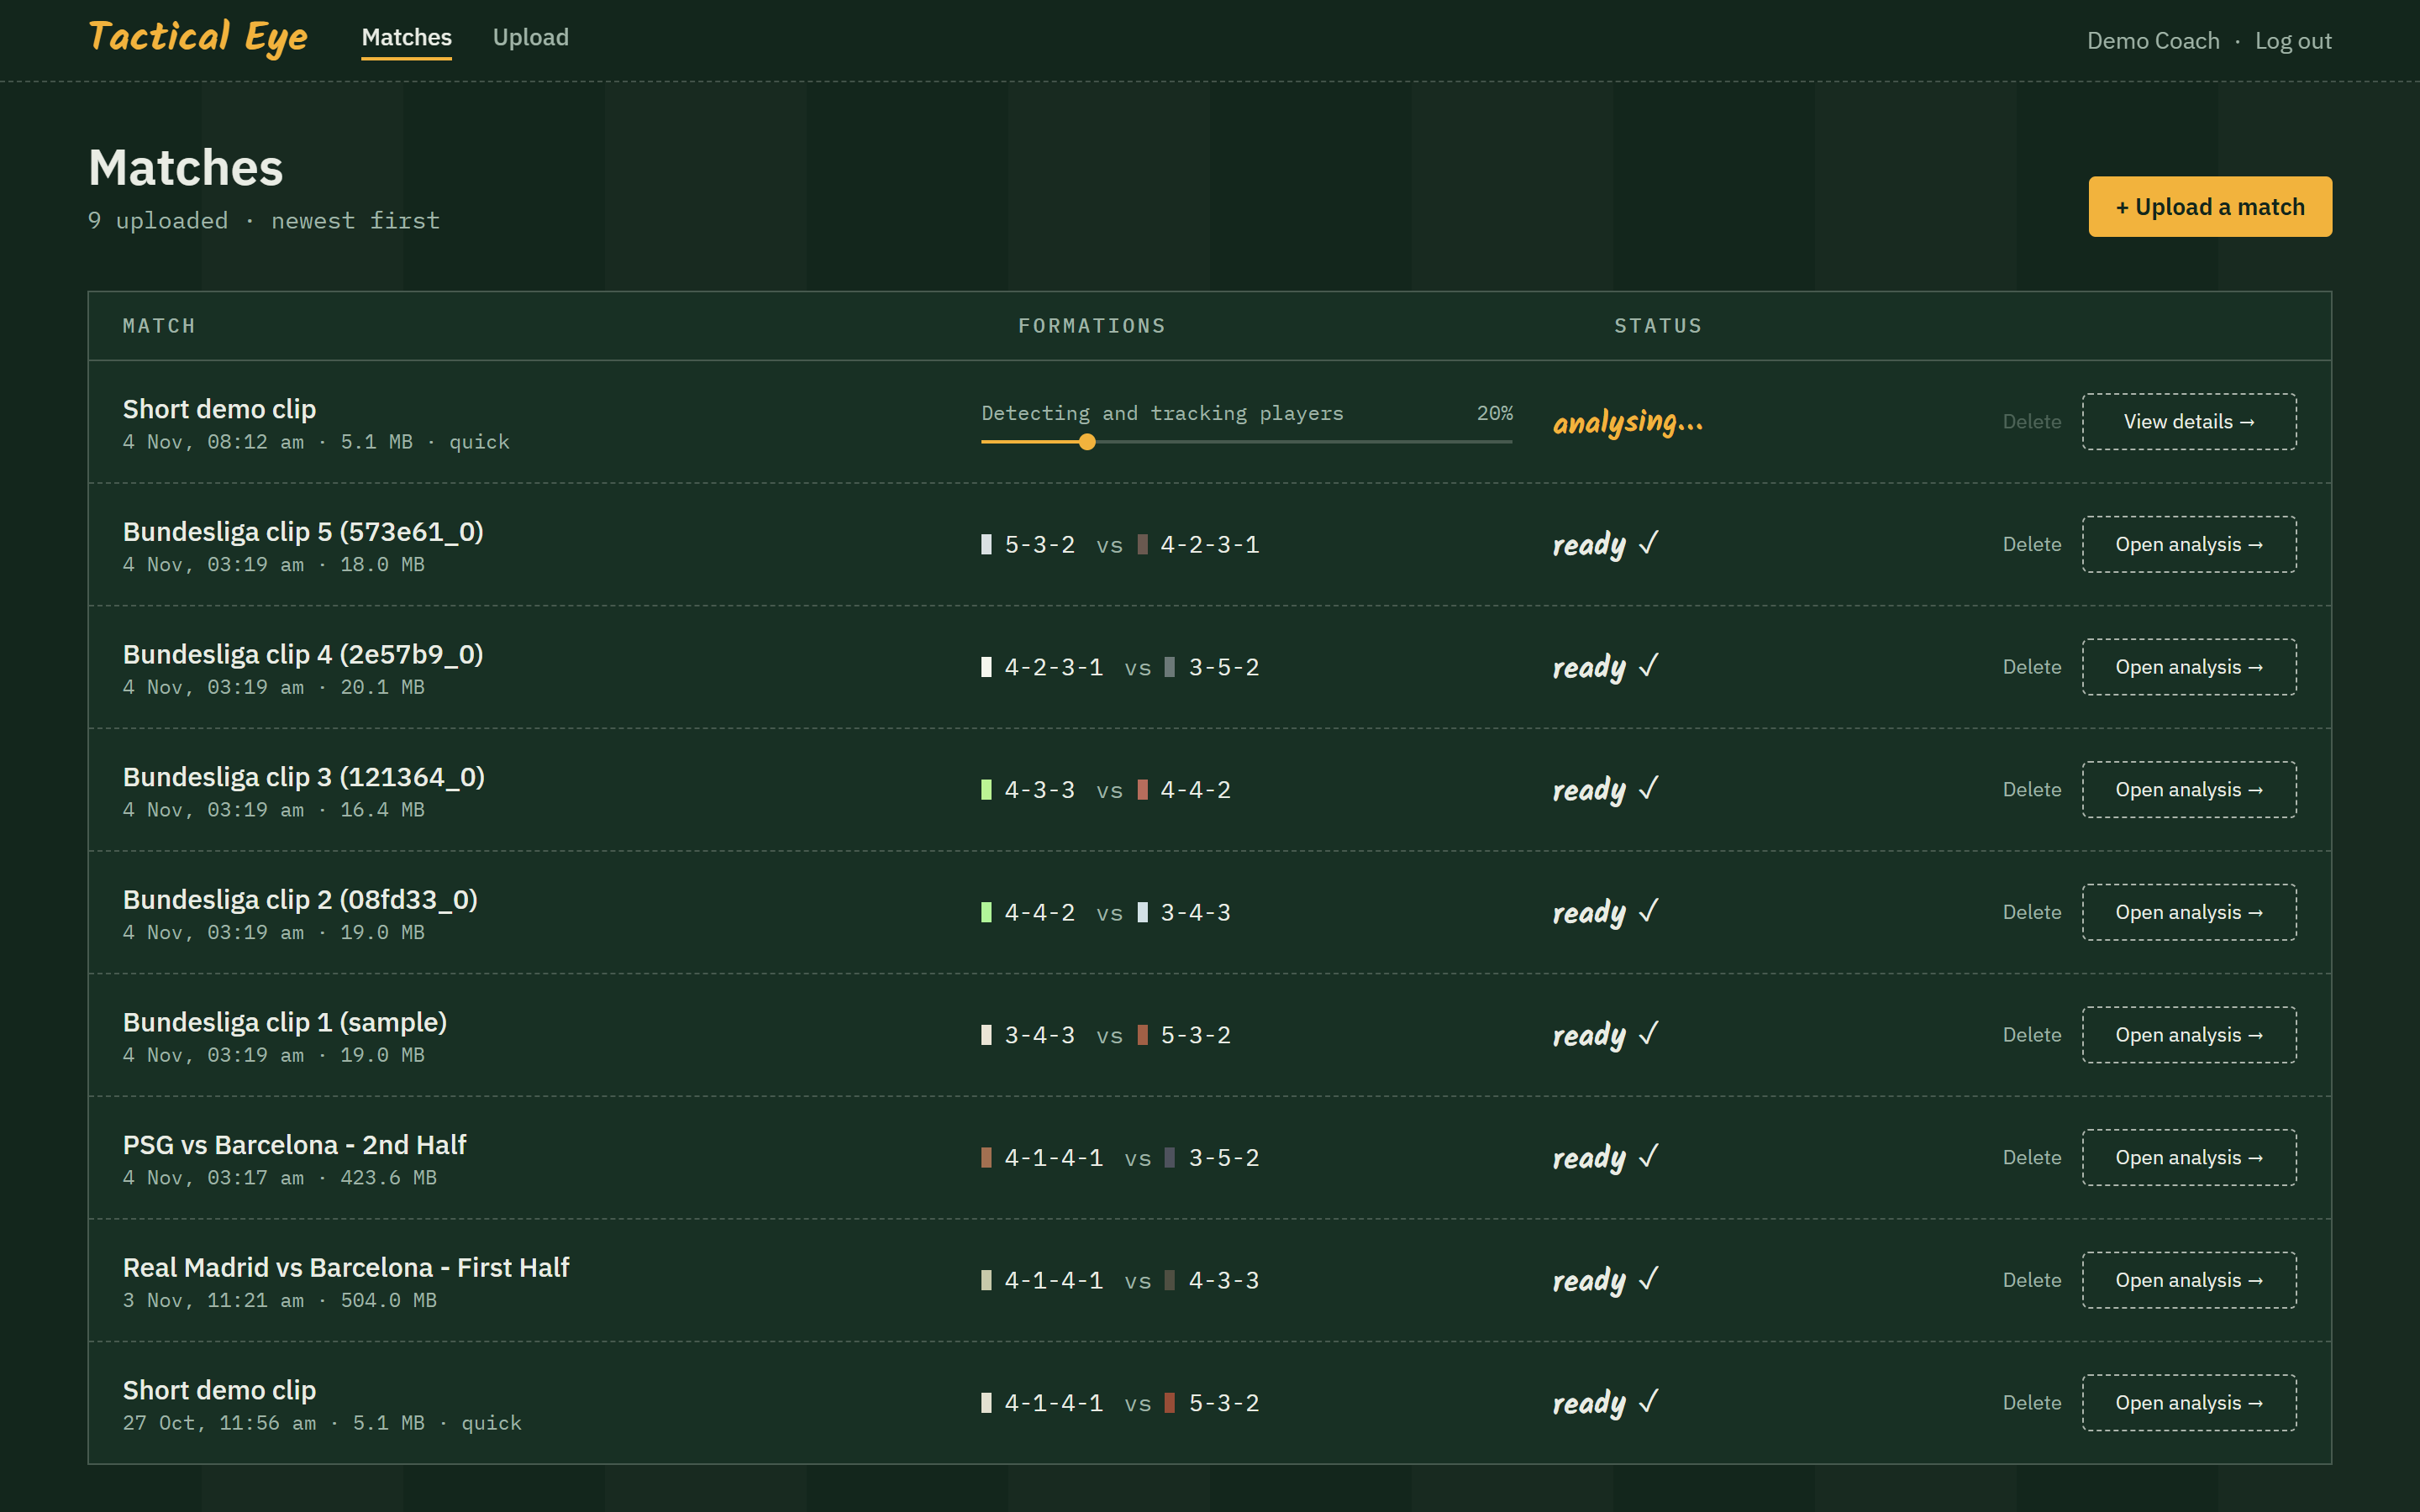
\includegraphics[width=\textwidth]{09_matches_live_progress}
	\caption{Live progress on the match list}
	\label{fig:list-progress}
\end{figure}

\begin{table}[H]
	\centering
	\begin{tabular}{|p{0.34\textwidth}|p{0.10\textwidth}|p{0.48\textwidth}|}
		\hline
		\textbf{Step} & \textbf{Progress} & \textbf{What happens} \\
		\hline
		Uploading video to GPU & 0--5\,\% & Only with the cloud GPU: the video is sent in 50\,MB pieces. \\
		\hline
		Preparing video for playback & 0--5\,\% & A browser-compatible copy of the video is made; the analysis reads this copy. \\
		\hline
		Detecting and tracking players & 5--60\,\% & Every person and the ball are found in each analysed frame and followed through the video. \\
		\hline
		Mapping positions to the pitch & 60--88\,\% & Pitch markings are recognised and positions converted to metres; people off the pitch and false balls are removed. \\
		\hline
		Assigning teams & 88--93\,\% & Players are split into two teams by shirt colour; referees are recognised by their kit. \\
		\hline
		Analysing tactics & 93--98\,\% & Tracks are joined, positions smoothed, formations, position labels and metrics computed. \\
		\hline
		Saving results & 98--100\,\% & The results are stored and the page switches to the analysis view. \\
		\hline
	\end{tabular}
	\caption{The steps shown in the progress bar}
	\label{tab:steps}
\end{table}

If a step fails, the worker tries the whole analysis once more after 10 seconds, and the bar shows \emph{Retrying after an error} in the meantime.

\emph{Cancel analysis} stops an analysis that was started by mistake, for example with the wrong video or in the wrong mode. After a confirmation, a queued analysis is cancelled at once; a running one shows \emph{Cancelling\dots} and stops within a few seconds, also on the cloud GPU. The match then shows the note in \autoref{fig:cancelled} and can be started again with \emph{Re-analyse}. Cancelling a \emph{re-analysis} of a finished match does not lose anything: the match simply goes back to its earlier results.

\begin{figure}[H]
	\centering
	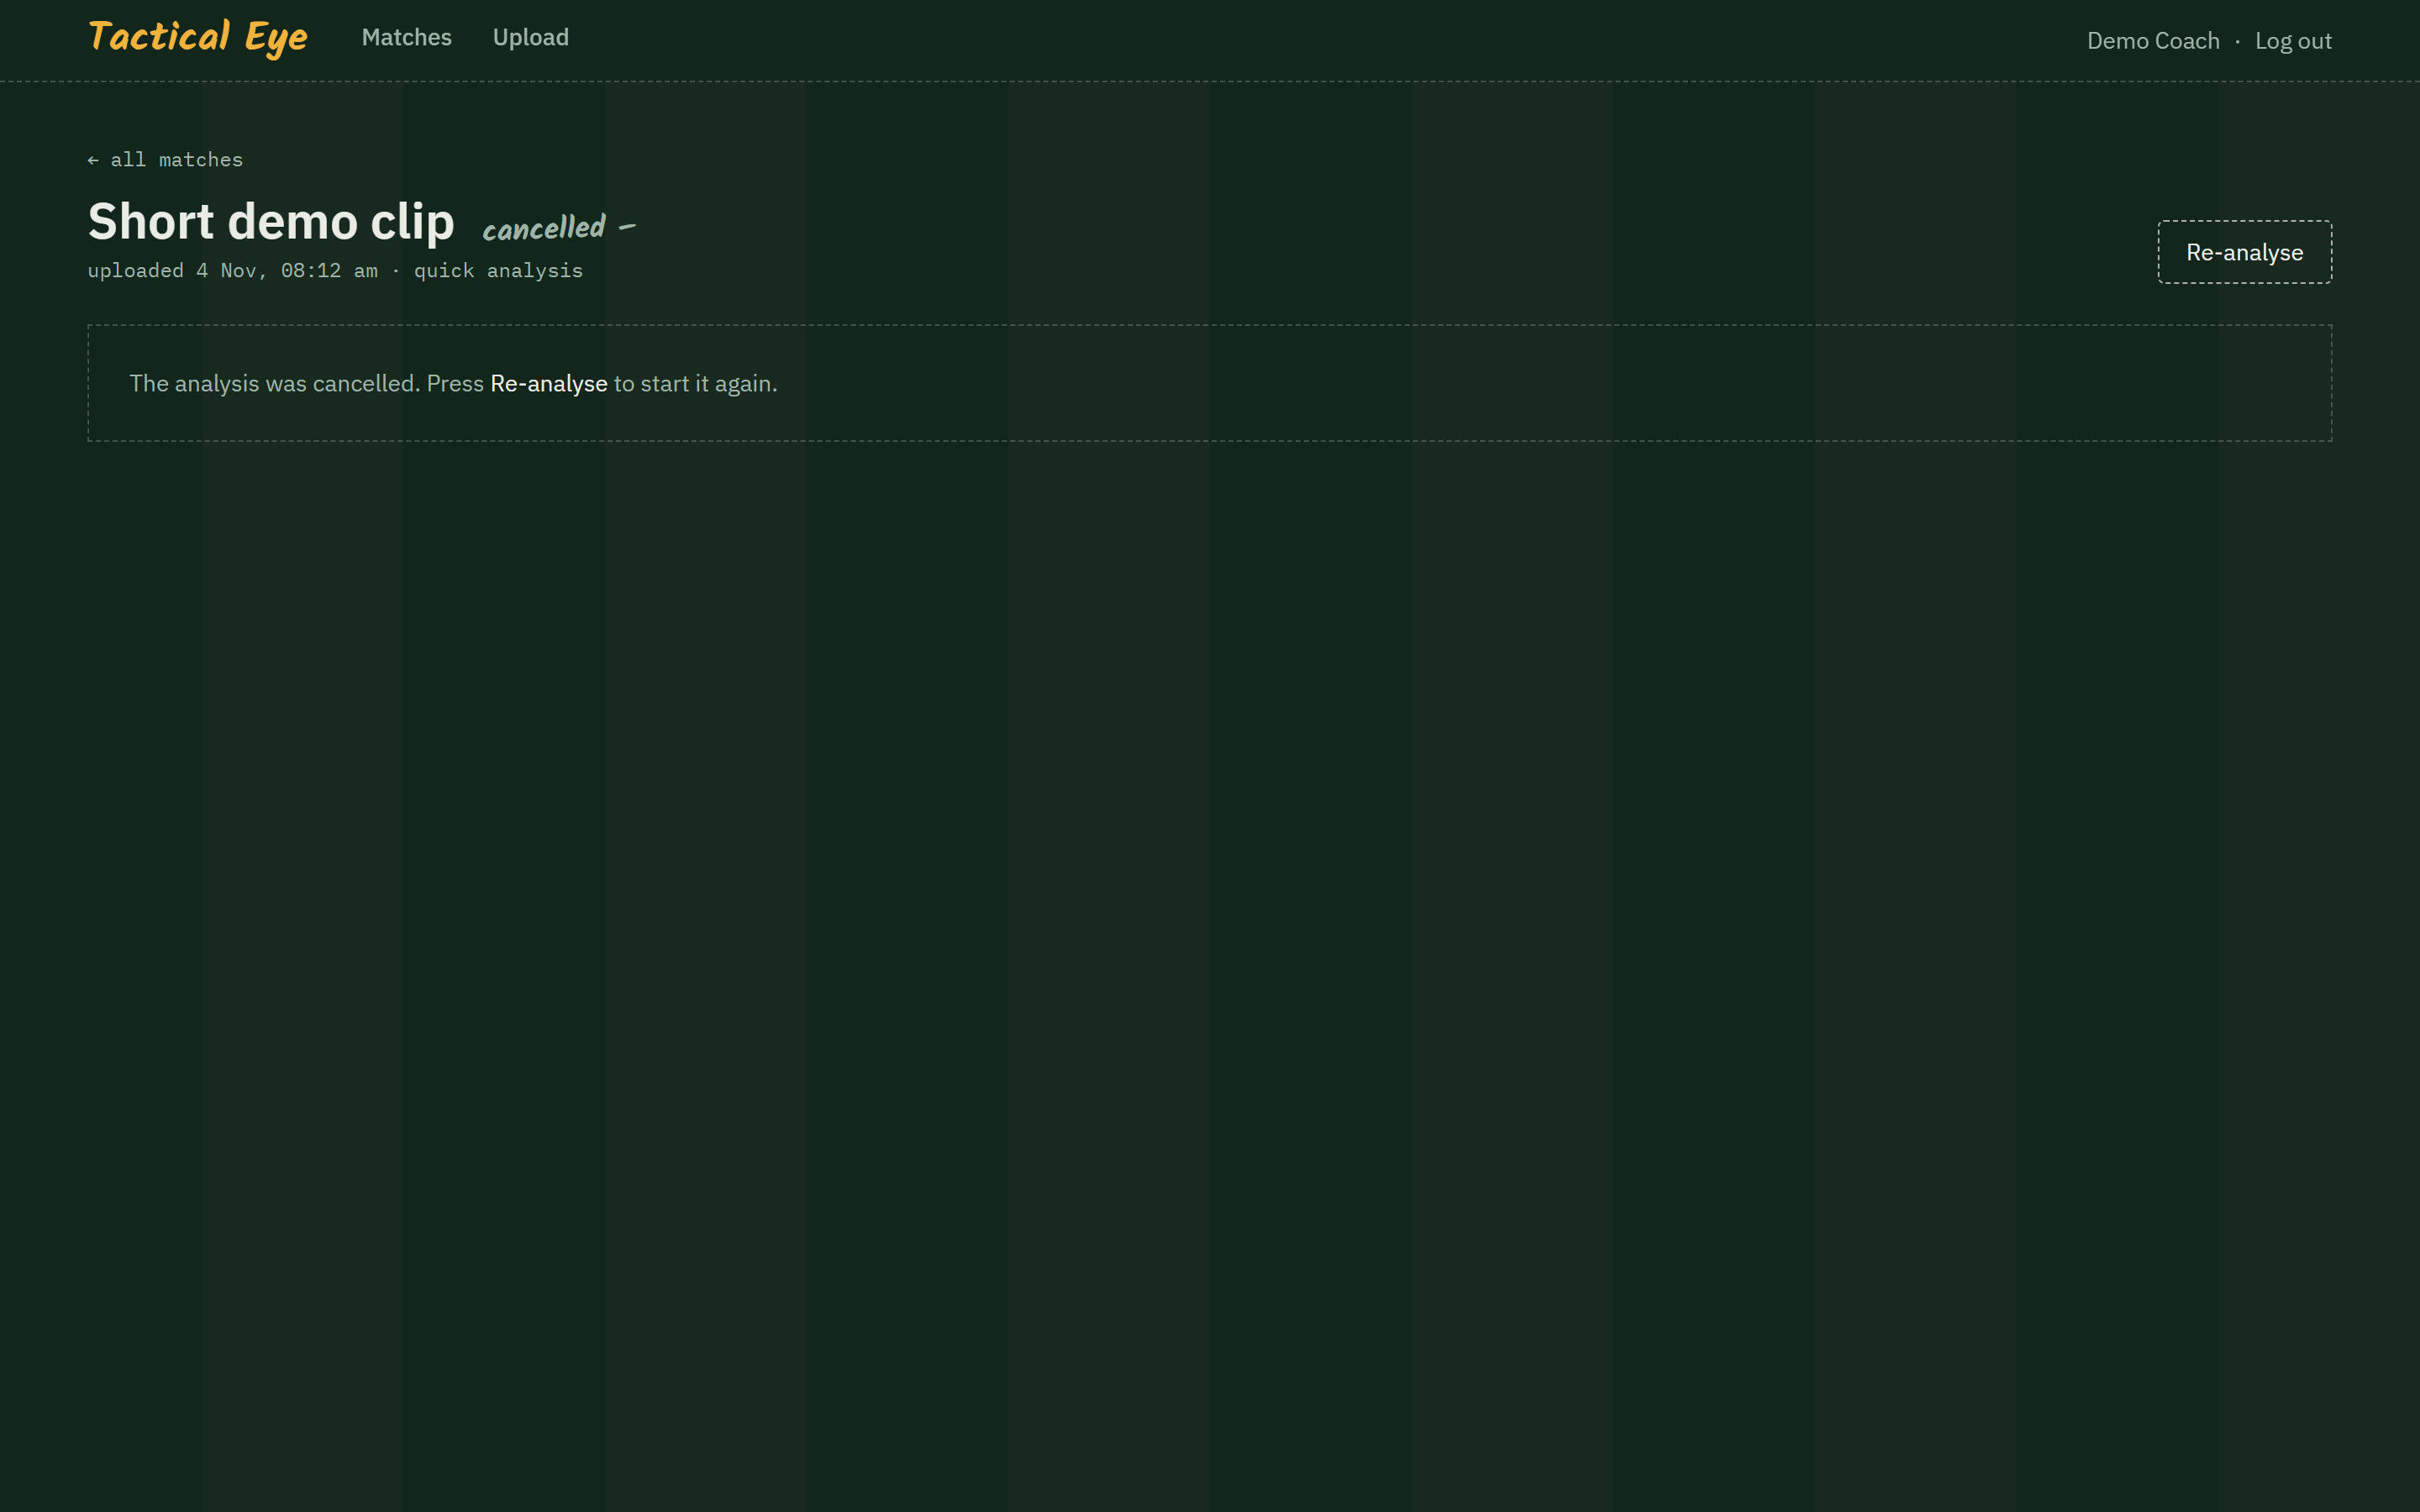
\includegraphics[width=\textwidth]{10_match_cancelled}
	\caption{A cancelled analysis}
	\label{fig:cancelled}
\end{figure}

\section{The analysis page}

When the analysis has finished, the match page shows the interactive analysis (\autoref{fig:intro-analysis} on page~\pageref{fig:intro-analysis}). Under the title, one line tells when the match was uploaded, in which mode it was analysed, and where and how long the processing took. The page has four parts: the video with its overlays and controls on the left, the tactical board with the current formations on the right, the layer buttons under the video, and three tabs further down with the summary, the selected player and the AI coaching report. \emph{Re-analyse} in the top right corner and \emph{$\leftarrow$ all matches} are described in \autoref{sec:reanalyse-delete}.

\subsection{Video player and controls}

The video plays inside the page. The browser's own controls are replaced by the controls under the video (\autoref{tab:video-controls}), because the drawings cover the video surface.

\begin{table}[H]
	\centering
	\begin{tabular}{|p{0.24\textwidth}|p{0.68\textwidth}|}
		\hline
		\textbf{Control} & \textbf{Action} \\
		\hline
		play / pause & Starts or pauses playback. Clicking an empty spot of the video does the same. \\
		\hline
		$\blacktriangleleft$ 1f / 1f $\blacktriangleright$ & Pauses and steps exactly one frame back or forward, for studying a situation. \\
		\hline
		Seek bar & Jumps to any moment; the time is shown as minutes:seconds.tenths. \\
		\hline
		Speed (1$\times$, 0.5$\times$, 0.25$\times$) & Slows playback down; the drawings stay in sync at every speed. \\
		\hline
		Full-screen button & In the bottom-right corner of the video. Shows the video, its drawings, the controls and the layer buttons on the whole screen (\autoref{fig:fullscreen}); the same button or Esc leaves full screen. \\
		\hline
	\end{tabular}
	\caption{Video controls}
	\label{tab:video-controls}
\end{table}

\begin{figure}[H]
	\centering
	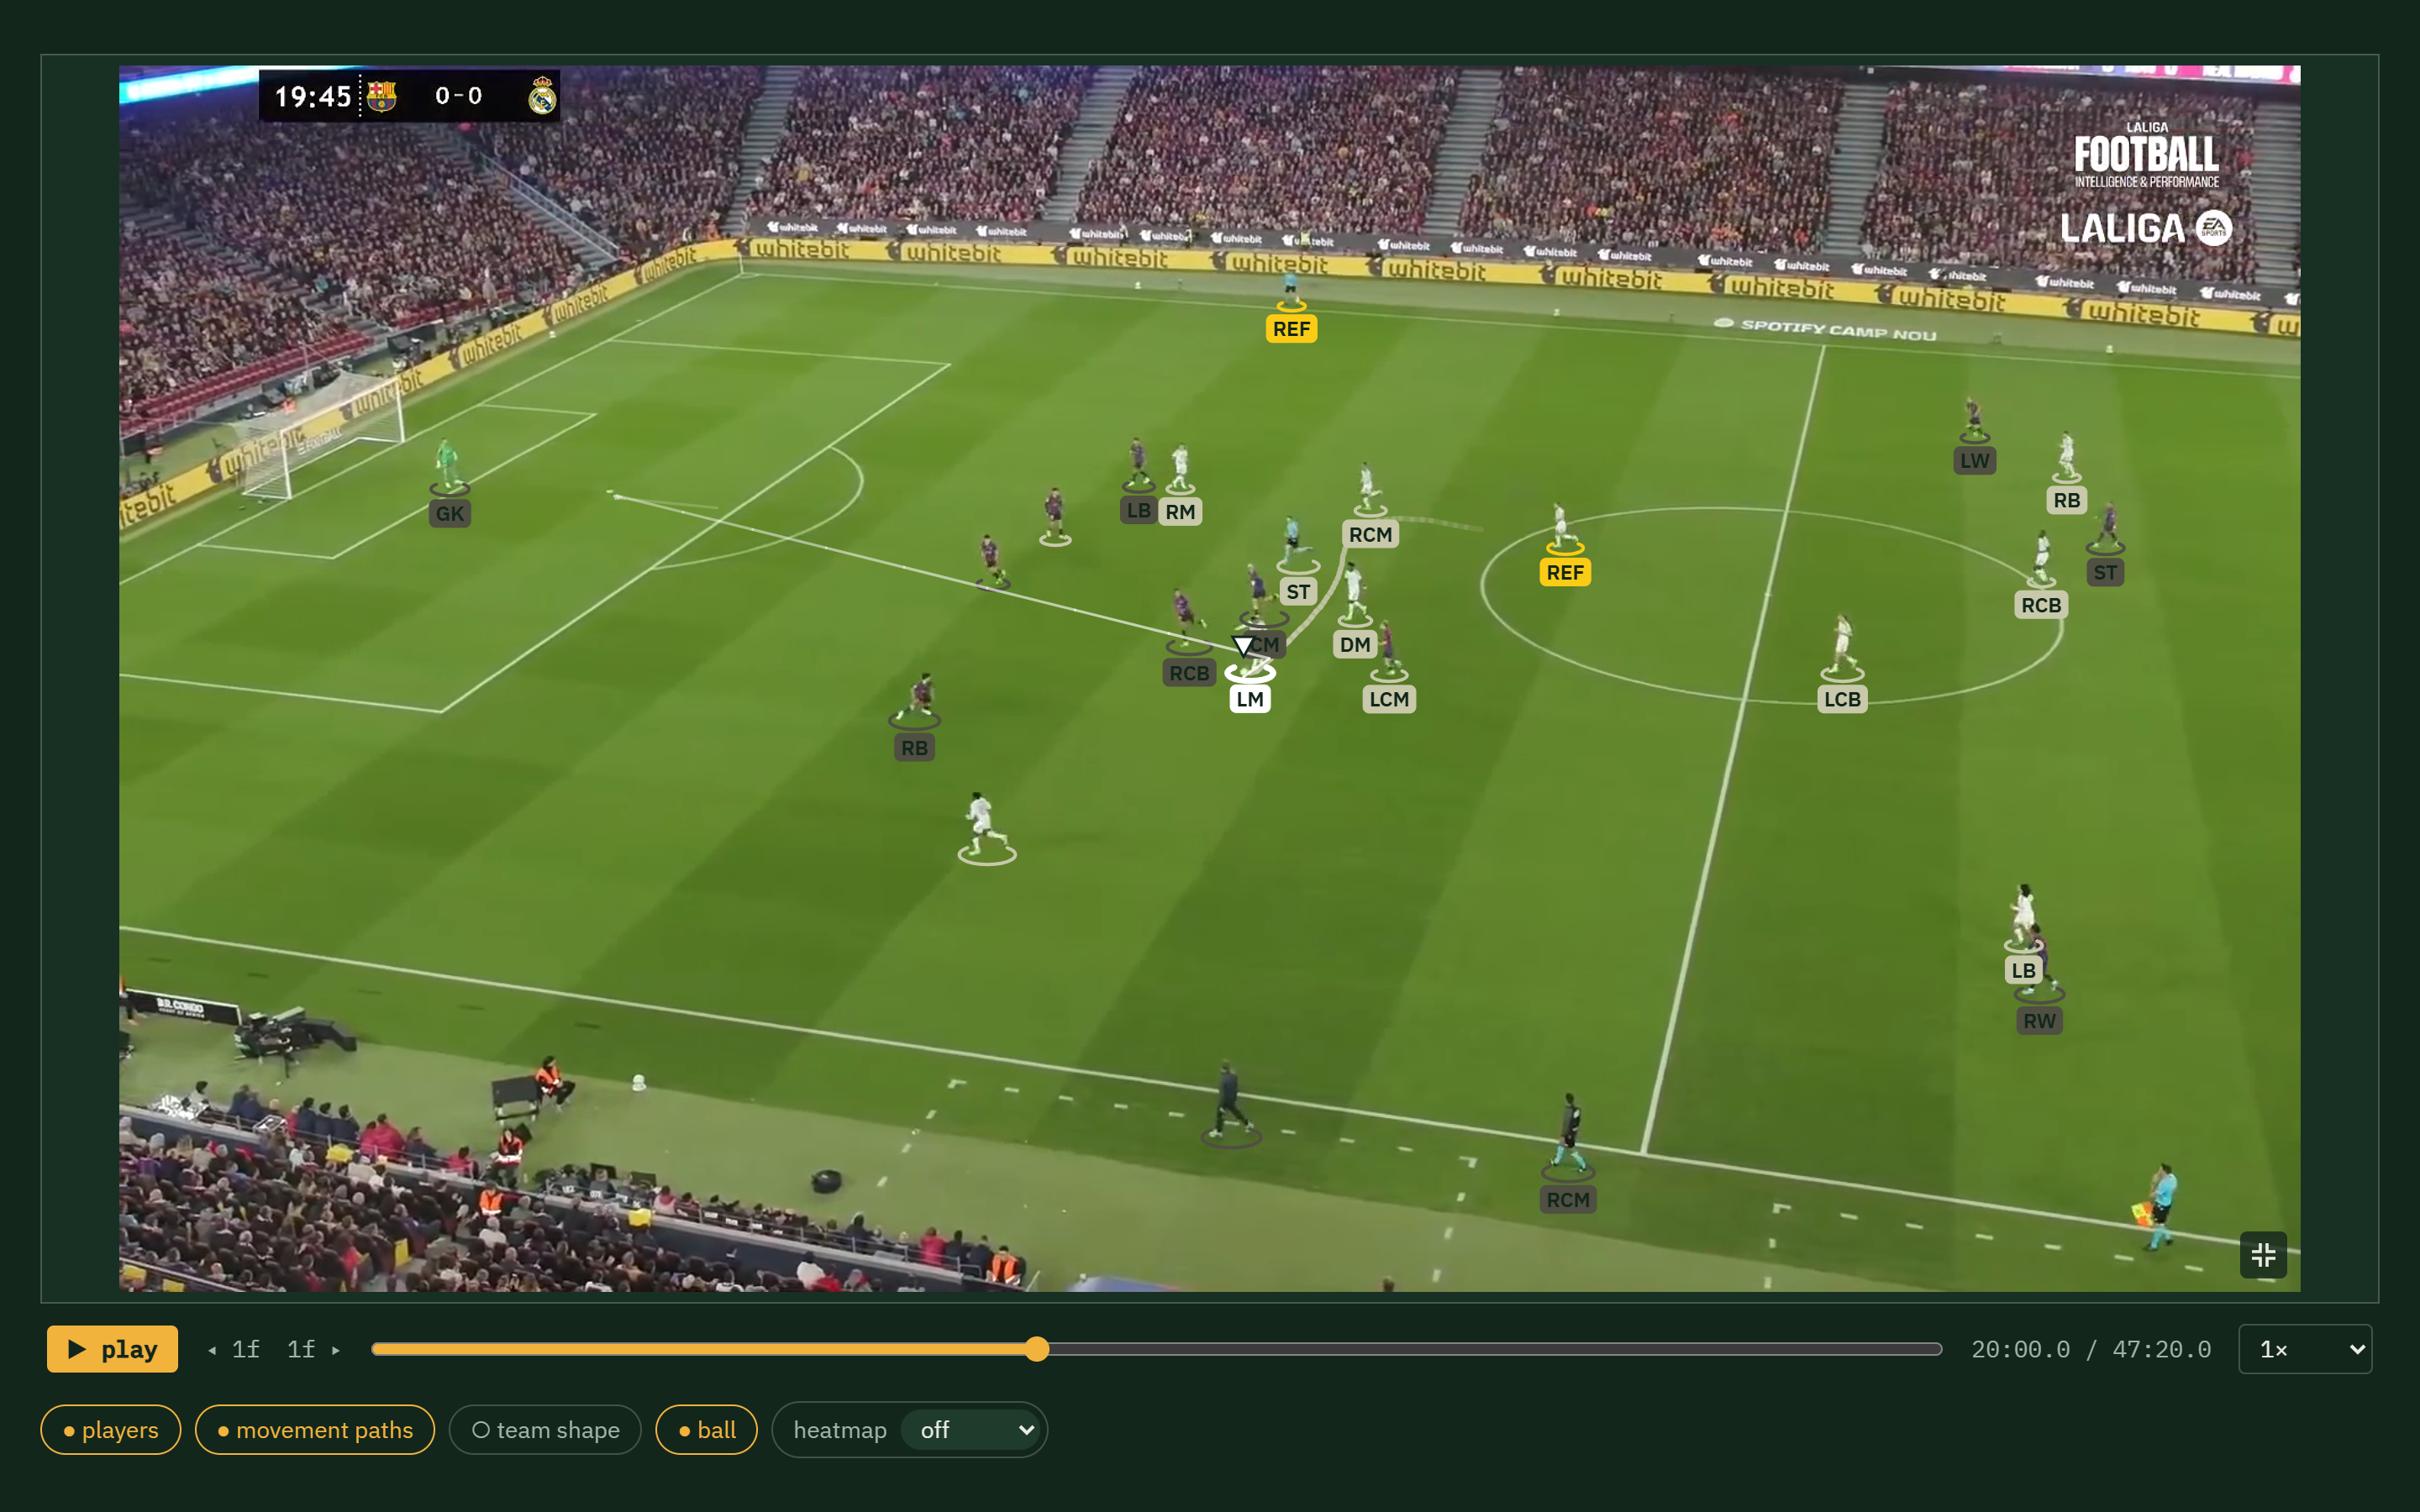
\includegraphics[width=\textwidth]{22_full_screen}
	\caption{Full-screen mode}
	\label{fig:fullscreen}
\end{figure}

All drawings follow the video frame by frame, also while the camera pans and zooms, because they are re-projected through the camera geometry of every frame (\autoref{sec:overlay-sync}).

\subsection{Overlay layers}

The layer buttons (\autoref{fig:layers}) switch the drawings on the video and on the board on and off; a filled dot means the layer is visible. \autoref{tab:layers} describes them.

\begin{figure}[H]
	\centering
	
\includegraphics[width=0.85\textwidth]{16_layer_controls}
	\caption{The layer buttons}
	\label{fig:layers}
\end{figure}

\begin{table}[H]
	\centering
	\begin{tabular}{|p{0.20\textwidth}|p{0.72\textwidth}|}
		\hline
		\textbf{Layer} & \textbf{What is drawn} \\
		\hline
		players & An ellipse at each person's feet in their kit colour with a label: the position (LB, RCB, DM, ST\dots) for players, GK for goalkeepers and REF for referees, in yellow. A player whose position is unknown at that moment gets only the ellipse. \\
		\hline
		movement paths & The path of the last 4 seconds, drawn on the grass and fading with age (\autoref{fig:paths}). When a player is selected, only their path is shown. \\
		\hline
		team shape & The area enclosed by each team's outfield players, filled in the team colour (\autoref{fig:shape}). A small area means a compact team. \\
		\hline
		ball & A marker above the ball and its path over the last 1.5 seconds. \\
		\hline
		heatmap (menu) & Off, Team A, Team B or Ball: where that team's players, or the ball, spent the most time over the whole video, from rarely (blue-green) to most often (red), painted onto the pitch (\autoref{fig:heatmaps}). \\
		\hline
	\end{tabular}
	\caption{Overlay layers}
	\label{tab:layers}
\end{table}

\begin{figure}[H]
	\centering
	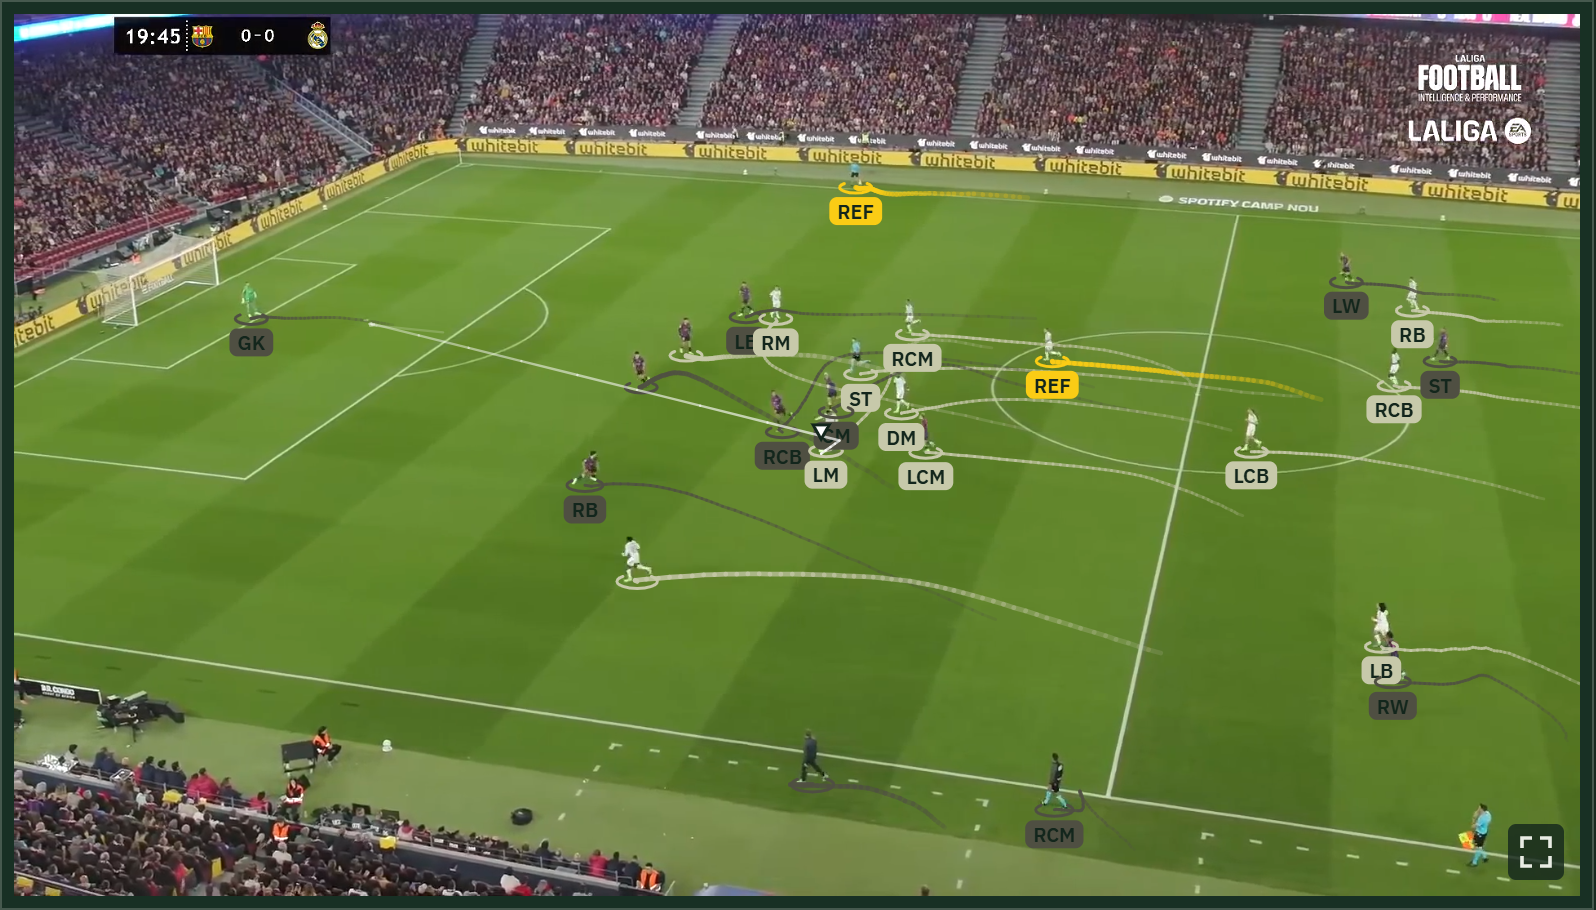
\includegraphics[width=\textwidth]{12_overlay_players_paths}
	\caption{Position labels and movement paths drawn on the video; the referees are labelled REF}
	\label{fig:paths}
\end{figure}

\begin{figure}[H]
	\centering
	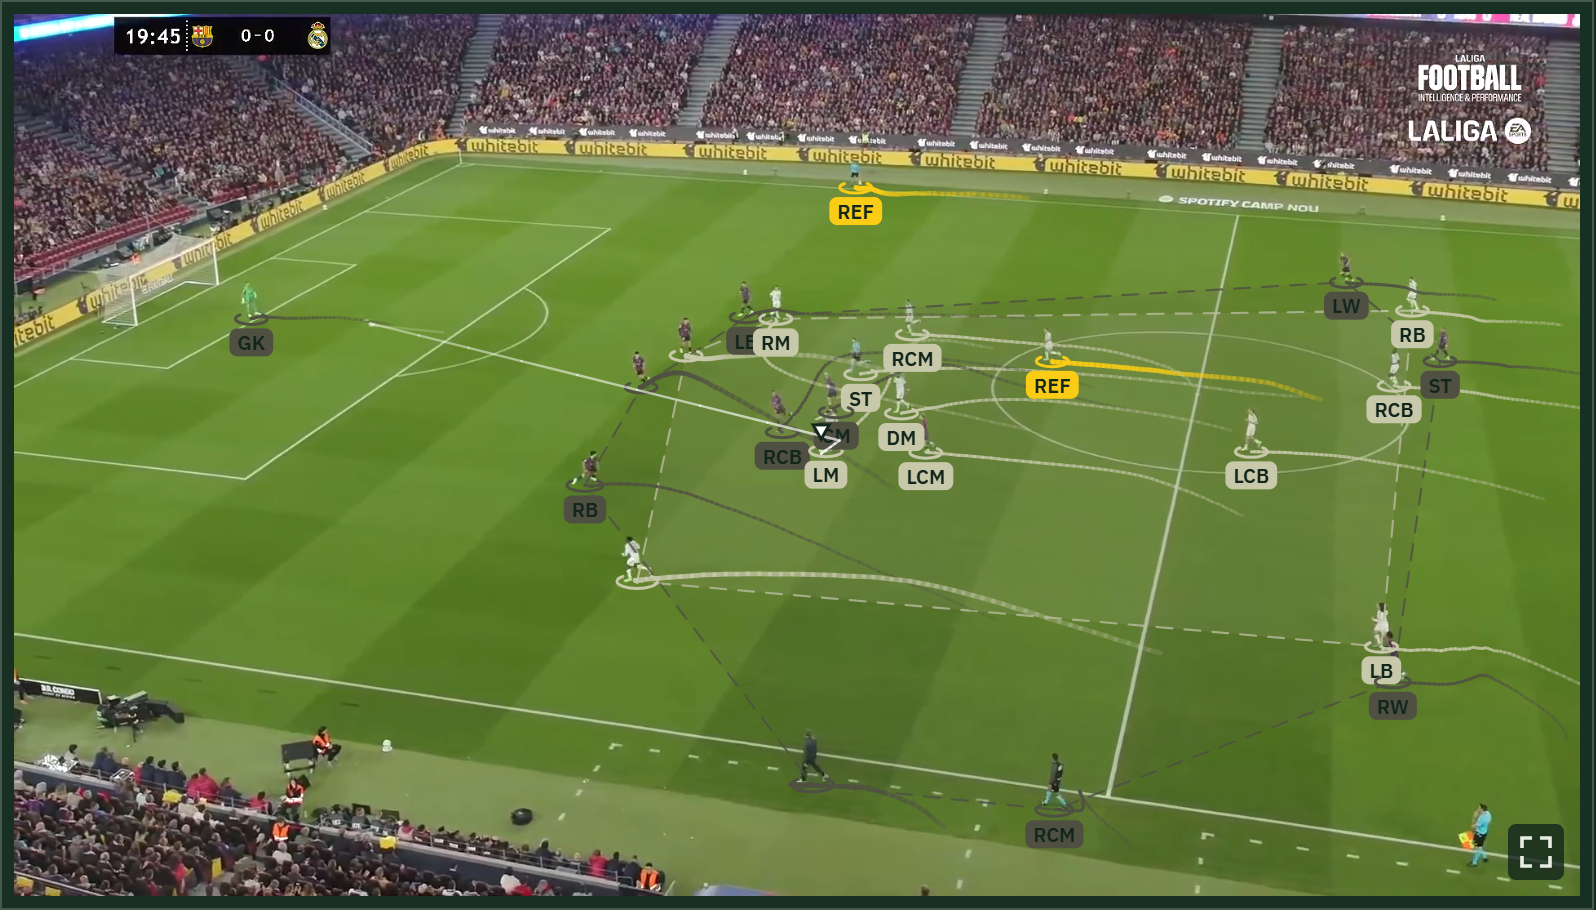
\includegraphics[width=\textwidth]{13_overlay_team_shape}
	\caption{The team shape layer}
	\label{fig:shape}
\end{figure}

\begin{figure}[H]
	\centering
	\begin{subfigure}{0.49\textwidth}
		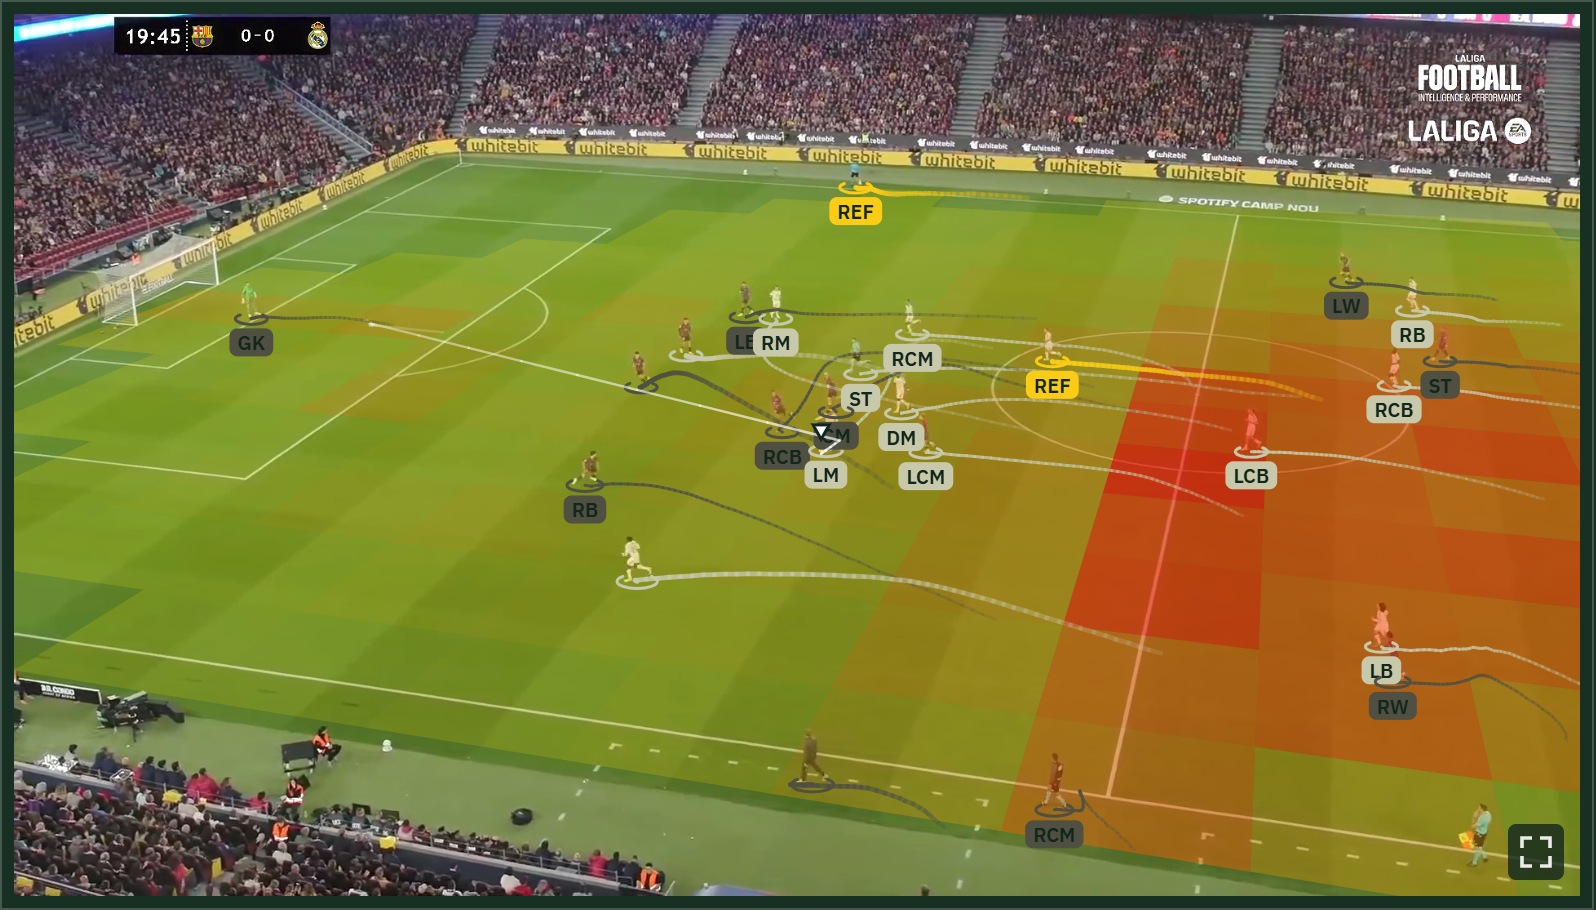
\includegraphics[width=\textwidth]{14_overlay_heatmap_team_a}
		\caption{Team A}
	\end{subfigure}
	\hfill
	\begin{subfigure}{0.49\textwidth}
		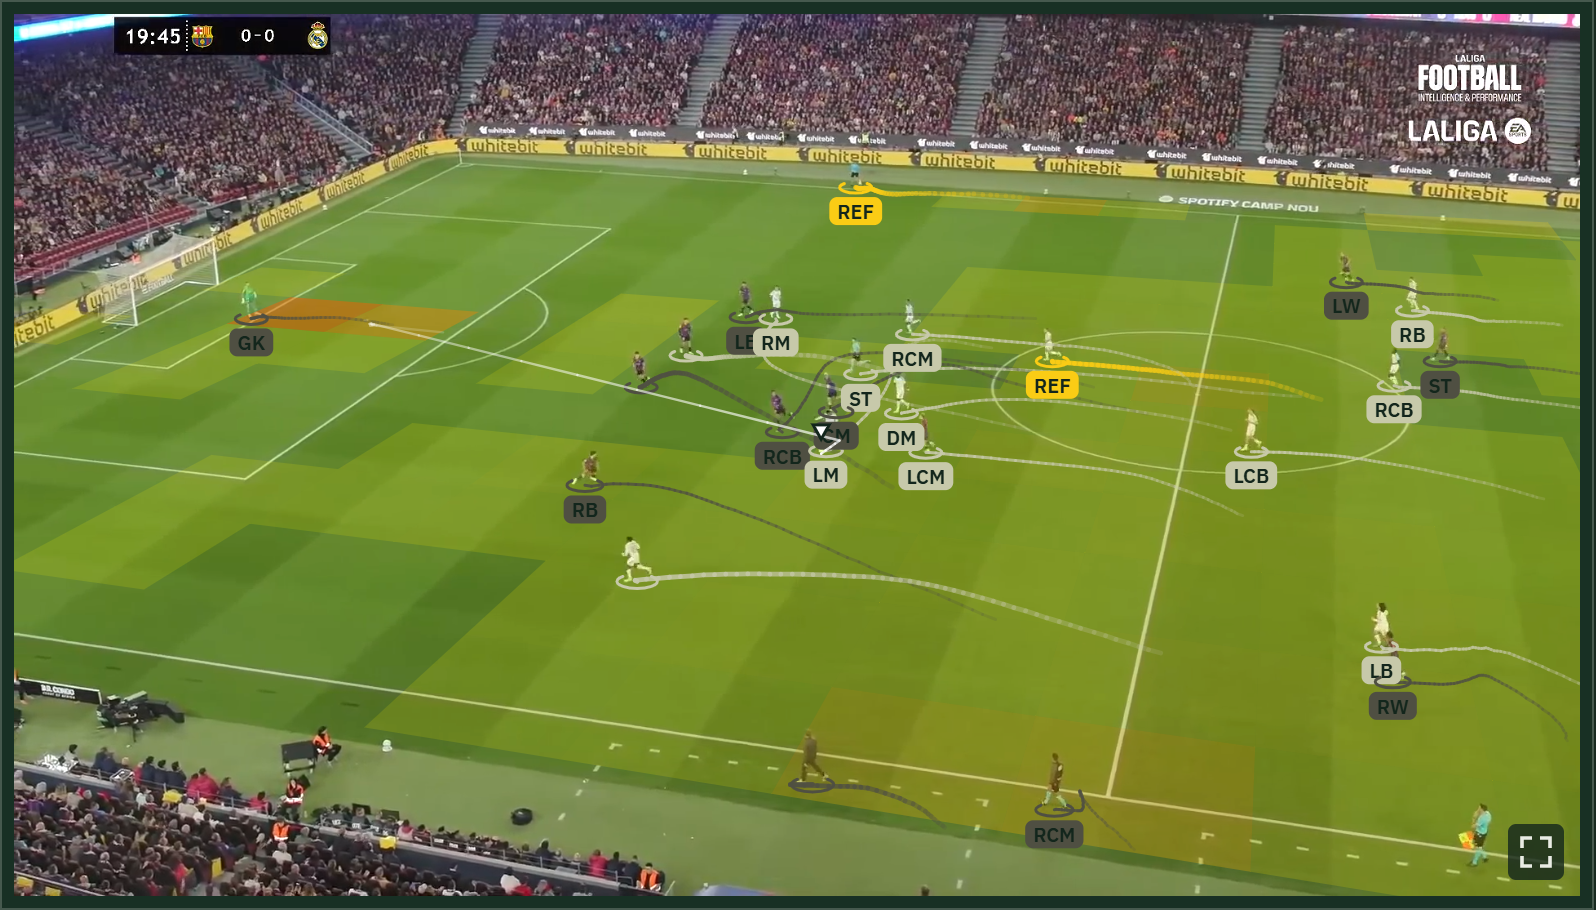
\includegraphics[width=\textwidth]{15_overlay_heatmap_ball}
		\caption{Ball}
	\end{subfigure}
	\caption{Heatmaps painted onto the pitch in the video}
	\label{fig:heatmaps}
\end{figure}

\subsection{Tactical board and formations}

The tactical board (\autoref{fig:board}) shows the same moment as the video from above, on a to-scale $105 \times 68$\,m pitch drawn like a chalkboard: Team A as circles, Team B as crosses, referees as small yellow squares and the ball as a white dot, each player with their position label. The board uses the same layers as the video. Unlike the video, it shows true metric proportions, so distances and spacing are easy to judge.

Under the board, two cards show the formation each team plays at the current moment, for example 3-4-3 and 4-2-3-1, with the runner-up, the second best fitting formation. A close runner-up means that the team's shape lies between two formations. Formations are worked out in 5-second windows, and a new one is only accepted once it has lasted about 20 seconds, so short wobbles do not count as changes.

\begin{figure}[H]
	\centering
	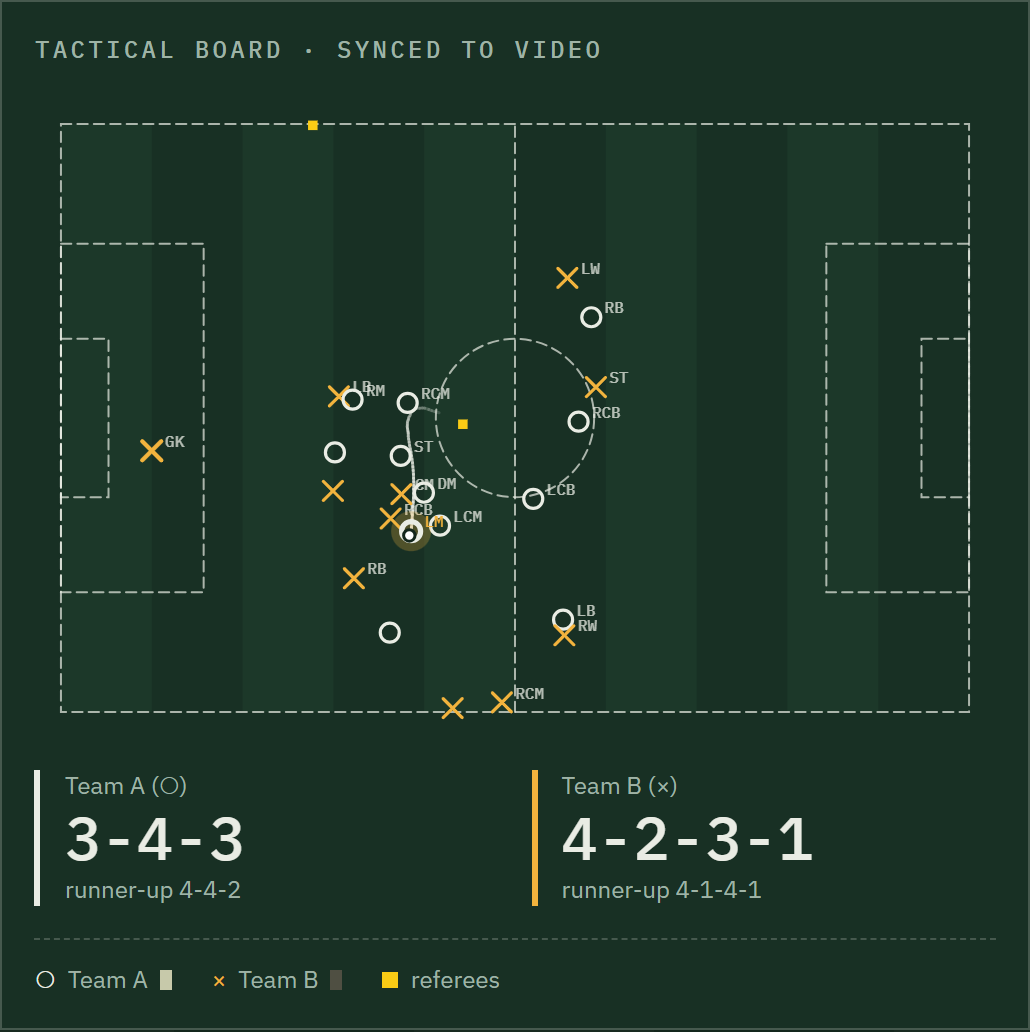
\includegraphics[width=0.6\textwidth]{18_board_and_formations}
	\caption{The tactical board with the current formations and the legend}
	\label{fig:board}
\end{figure}

\subsection{Inspecting a position}

Clicking a player on the video or on the board selects them: their marker is highlighted, their path is shown, and the \emph{Player} tab opens with the name of the position, for example ``Team A $\cdot$ LM'' (\autoref{fig:player-panel}). The tab shows a small pitch with the heatmap and the path of that position over the whole video, the distance covered, the time visible, the average speed and the top speed. The top speed is the best average over one second, not the fastest single step, which would be distorted by measurement noise (\autoref{sec:metrics}).

These numbers belong to the \emph{position}, not to a named player. One broadcast camera cannot follow the same player through a whole match (\autoref{sec:positions}), so the left back's statistics cover whoever played left back while visible. Clicking the same player again, or \emph{clear selection}, removes the selection.

\begin{figure}[H]
	\centering
	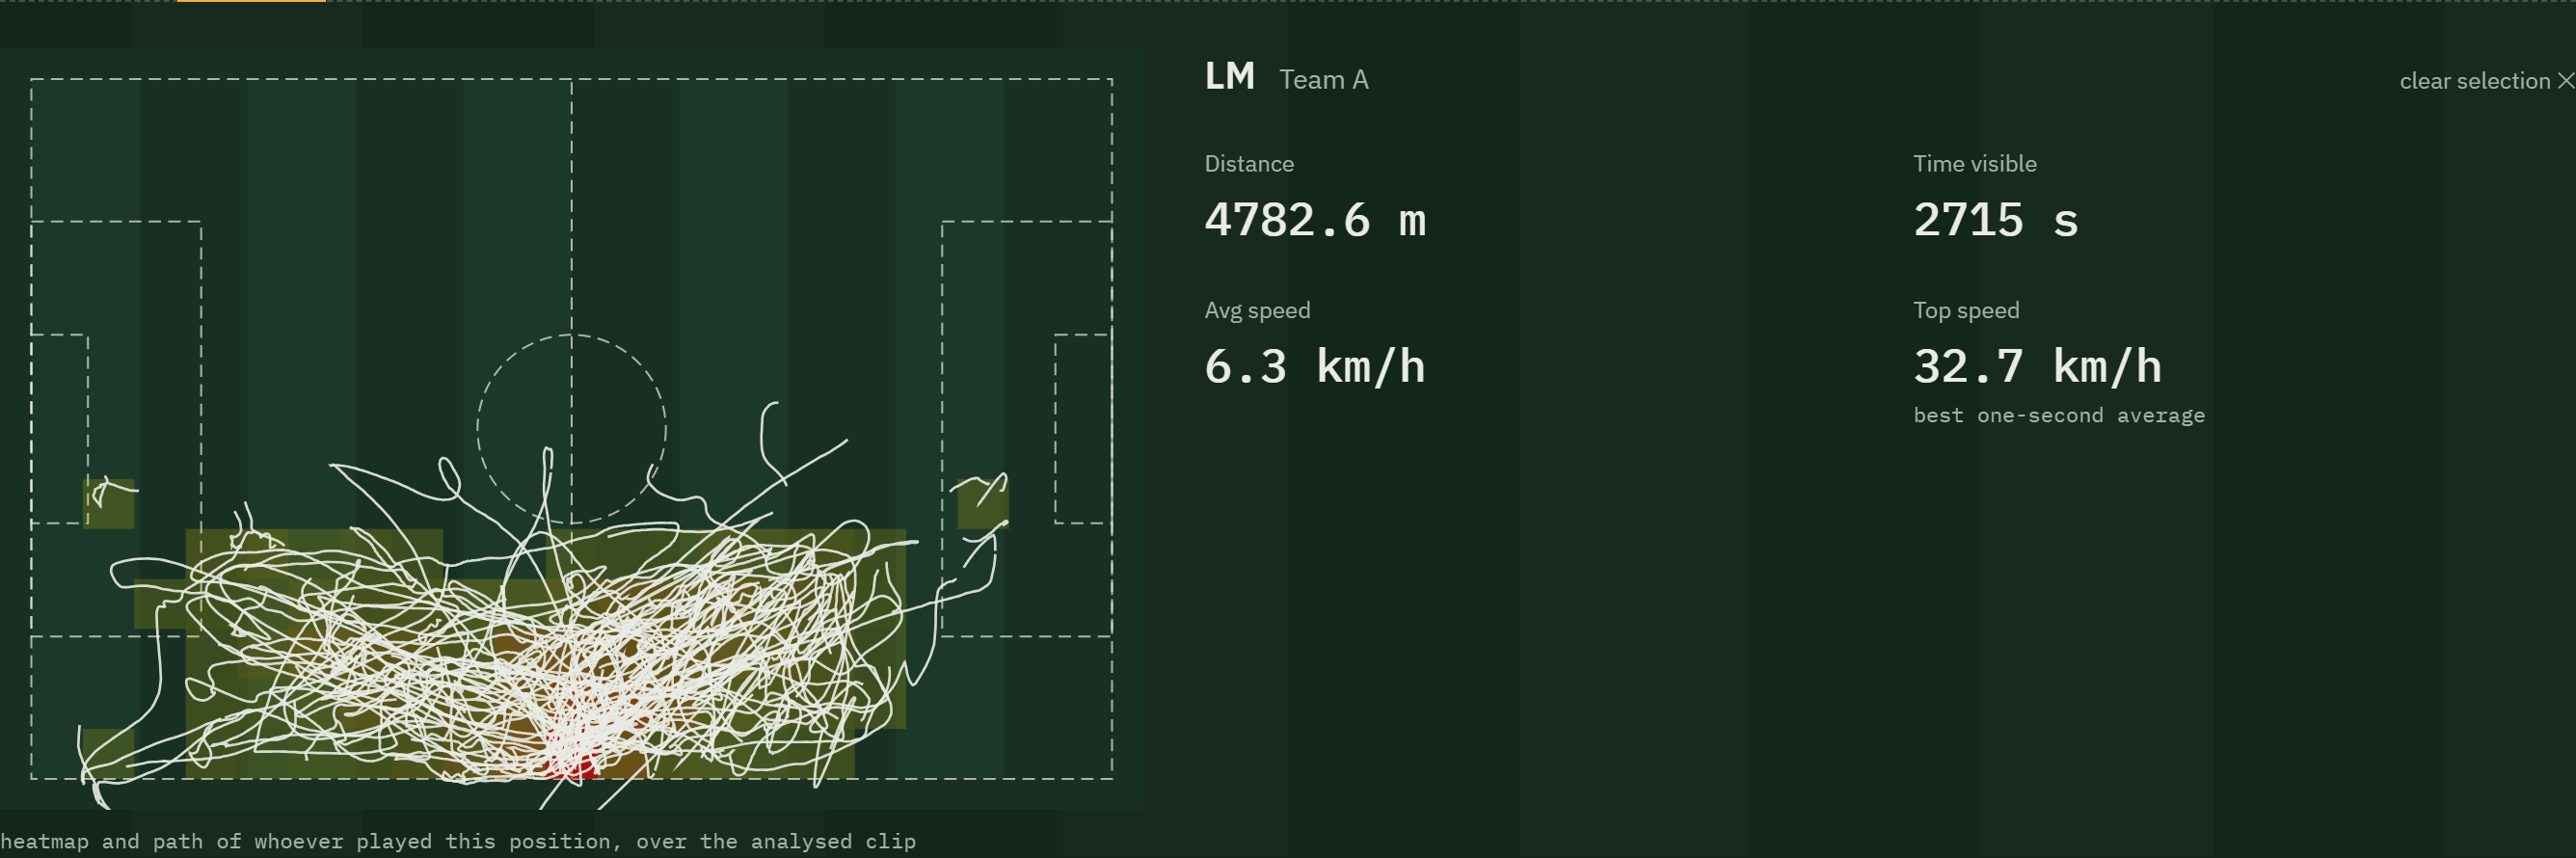
\includegraphics[width=\textwidth]{19_player_panel}
	\caption{The \emph{Player} tab of the left midfielder (LM) of Team A over a full half}
	\label{fig:player-panel}
\end{figure}

\subsection{Summary}

The \emph{Summary} tab (\autoref{fig:summary}) compares the two teams side by side. \autoref{tab:summary-metrics} explains the rows. Under the table, four numbers describe the video: its length, the number of frames analysed, the share of analysed frames in which the ball was found, and the number of formation changes.

\begin{figure}[H]
	\centering
	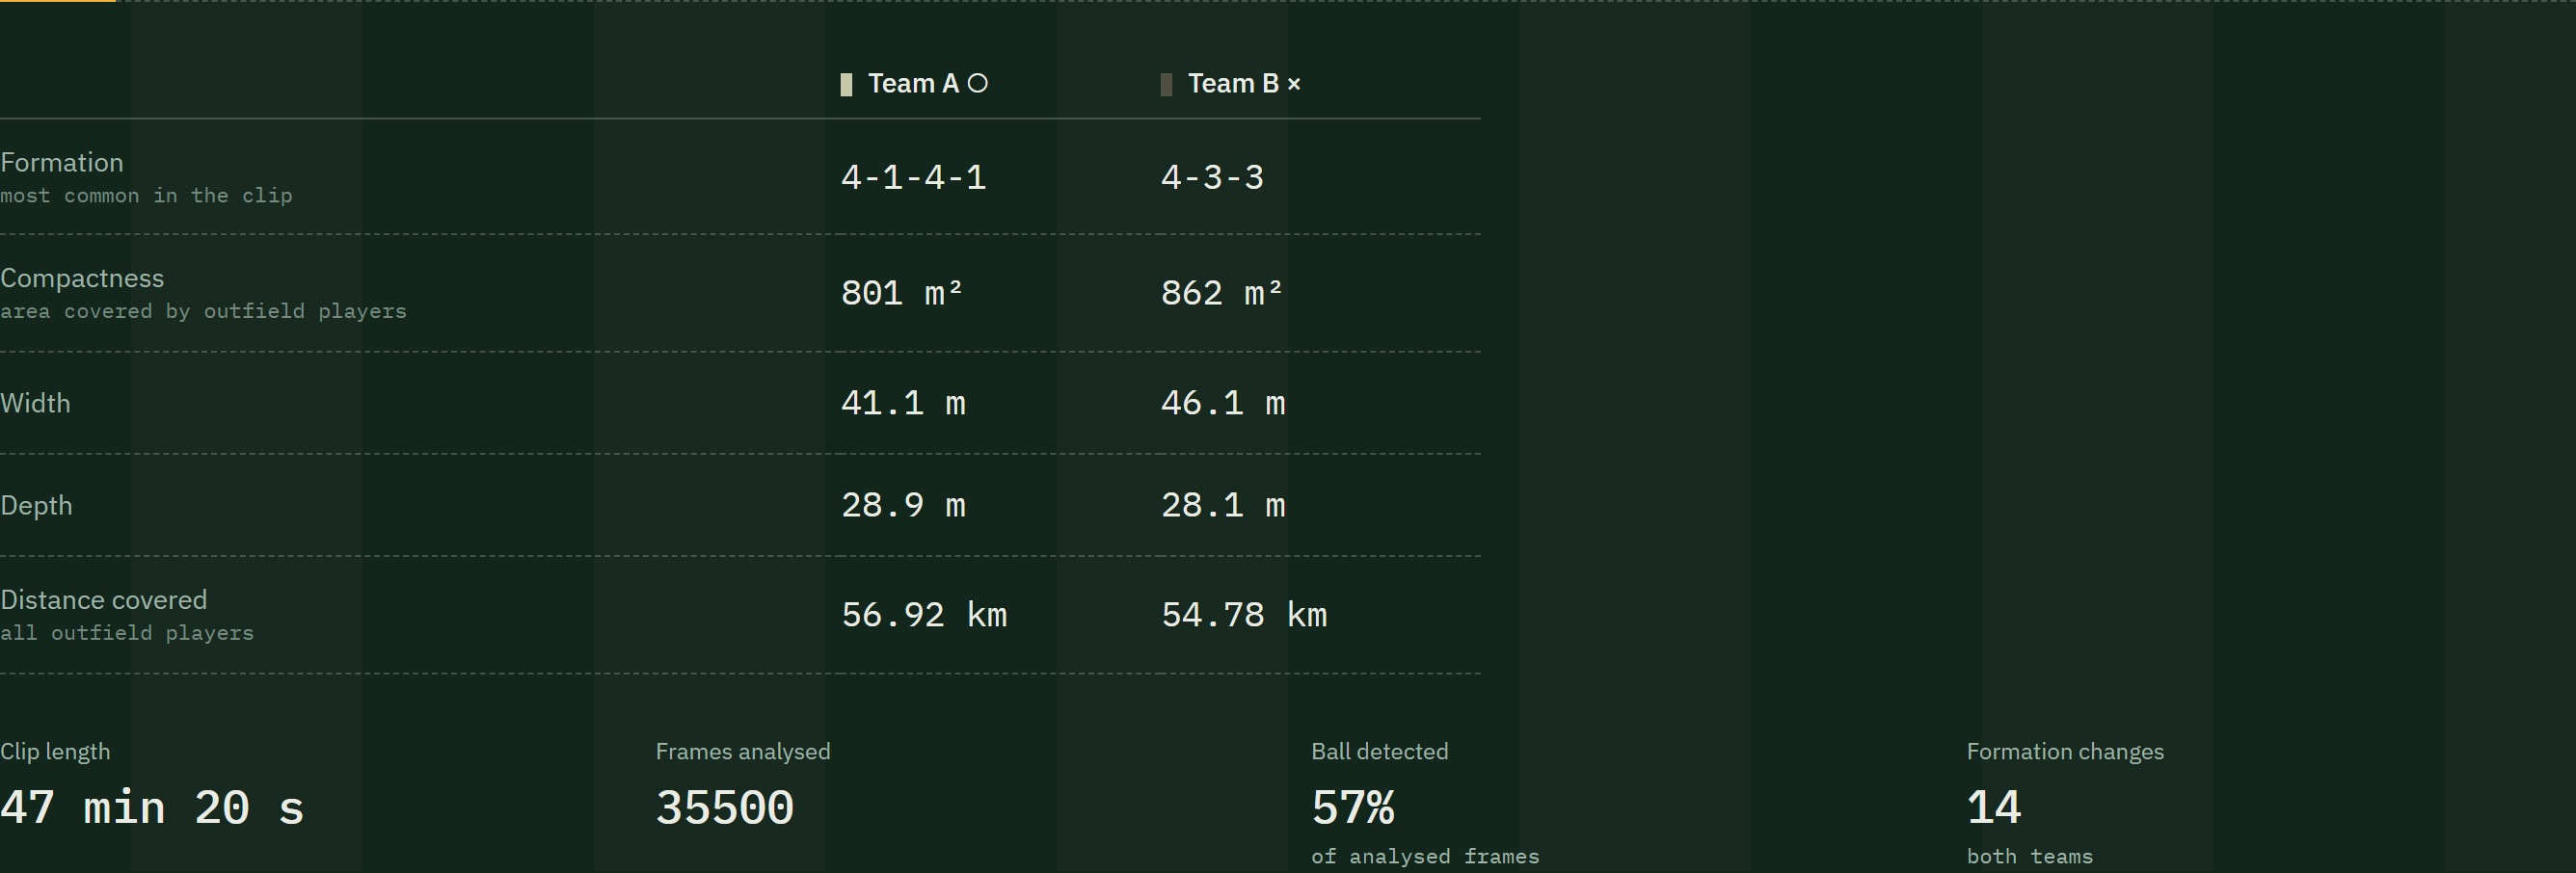
\includegraphics[width=\textwidth]{20_summary}
	\caption{The summary of the first half}
	\label{fig:summary}
\end{figure}

\begin{table}[H]
	\centering
	\begin{tabular}{|p{0.22\textwidth}|p{0.70\textwidth}|}
		\hline
		\textbf{Row} & \textbf{Meaning} \\
		\hline
		Formation & The team's most frequent formation in the video. \\
		\hline
		Compactness & Average area (m\textsuperscript{2}) enclosed by the outfield players. Smaller means the team stays closer together, typical of defending. \\
		\hline
		Width & Average distance (m) between the team's outermost players across the pitch. \\
		\hline
		Depth & Average distance (m) between the team's deepest and most advanced players. \\
		\hline
		Distance covered & Total distance run by the outfield players while visible, in km. \\
		\hline
	\end{tabular}
	\caption{Team metrics in the summary}
	\label{tab:summary-metrics}
\end{table}

\subsection{AI coaching report}

The \emph{AI coaching report} tab turns the statistics into a short written analysis (\autoref{fig:report}). \emph{Generate report} produces it in about 10--30 seconds, with the sections Overview, Team A, Team B, Shape over time, Recommendations and Data limitations. The report is stored with the match and shown at once the next time; \emph{Regenerate} writes a new version.

The report names the teams by their kit colour, such as ``Team A (white)'', and players by their position, such as the left back (LB). It is based only on the measured numbers: formations over time, compactness, width and depth in each third of the video, and the positions that ran the furthest. It is told not to invent events that are not measured, such as passes or goals, and to state the limits of the data. It is a starting point for the coach's own analysis, not a replacement for it.

\begin{figure}[H]
	\centering
	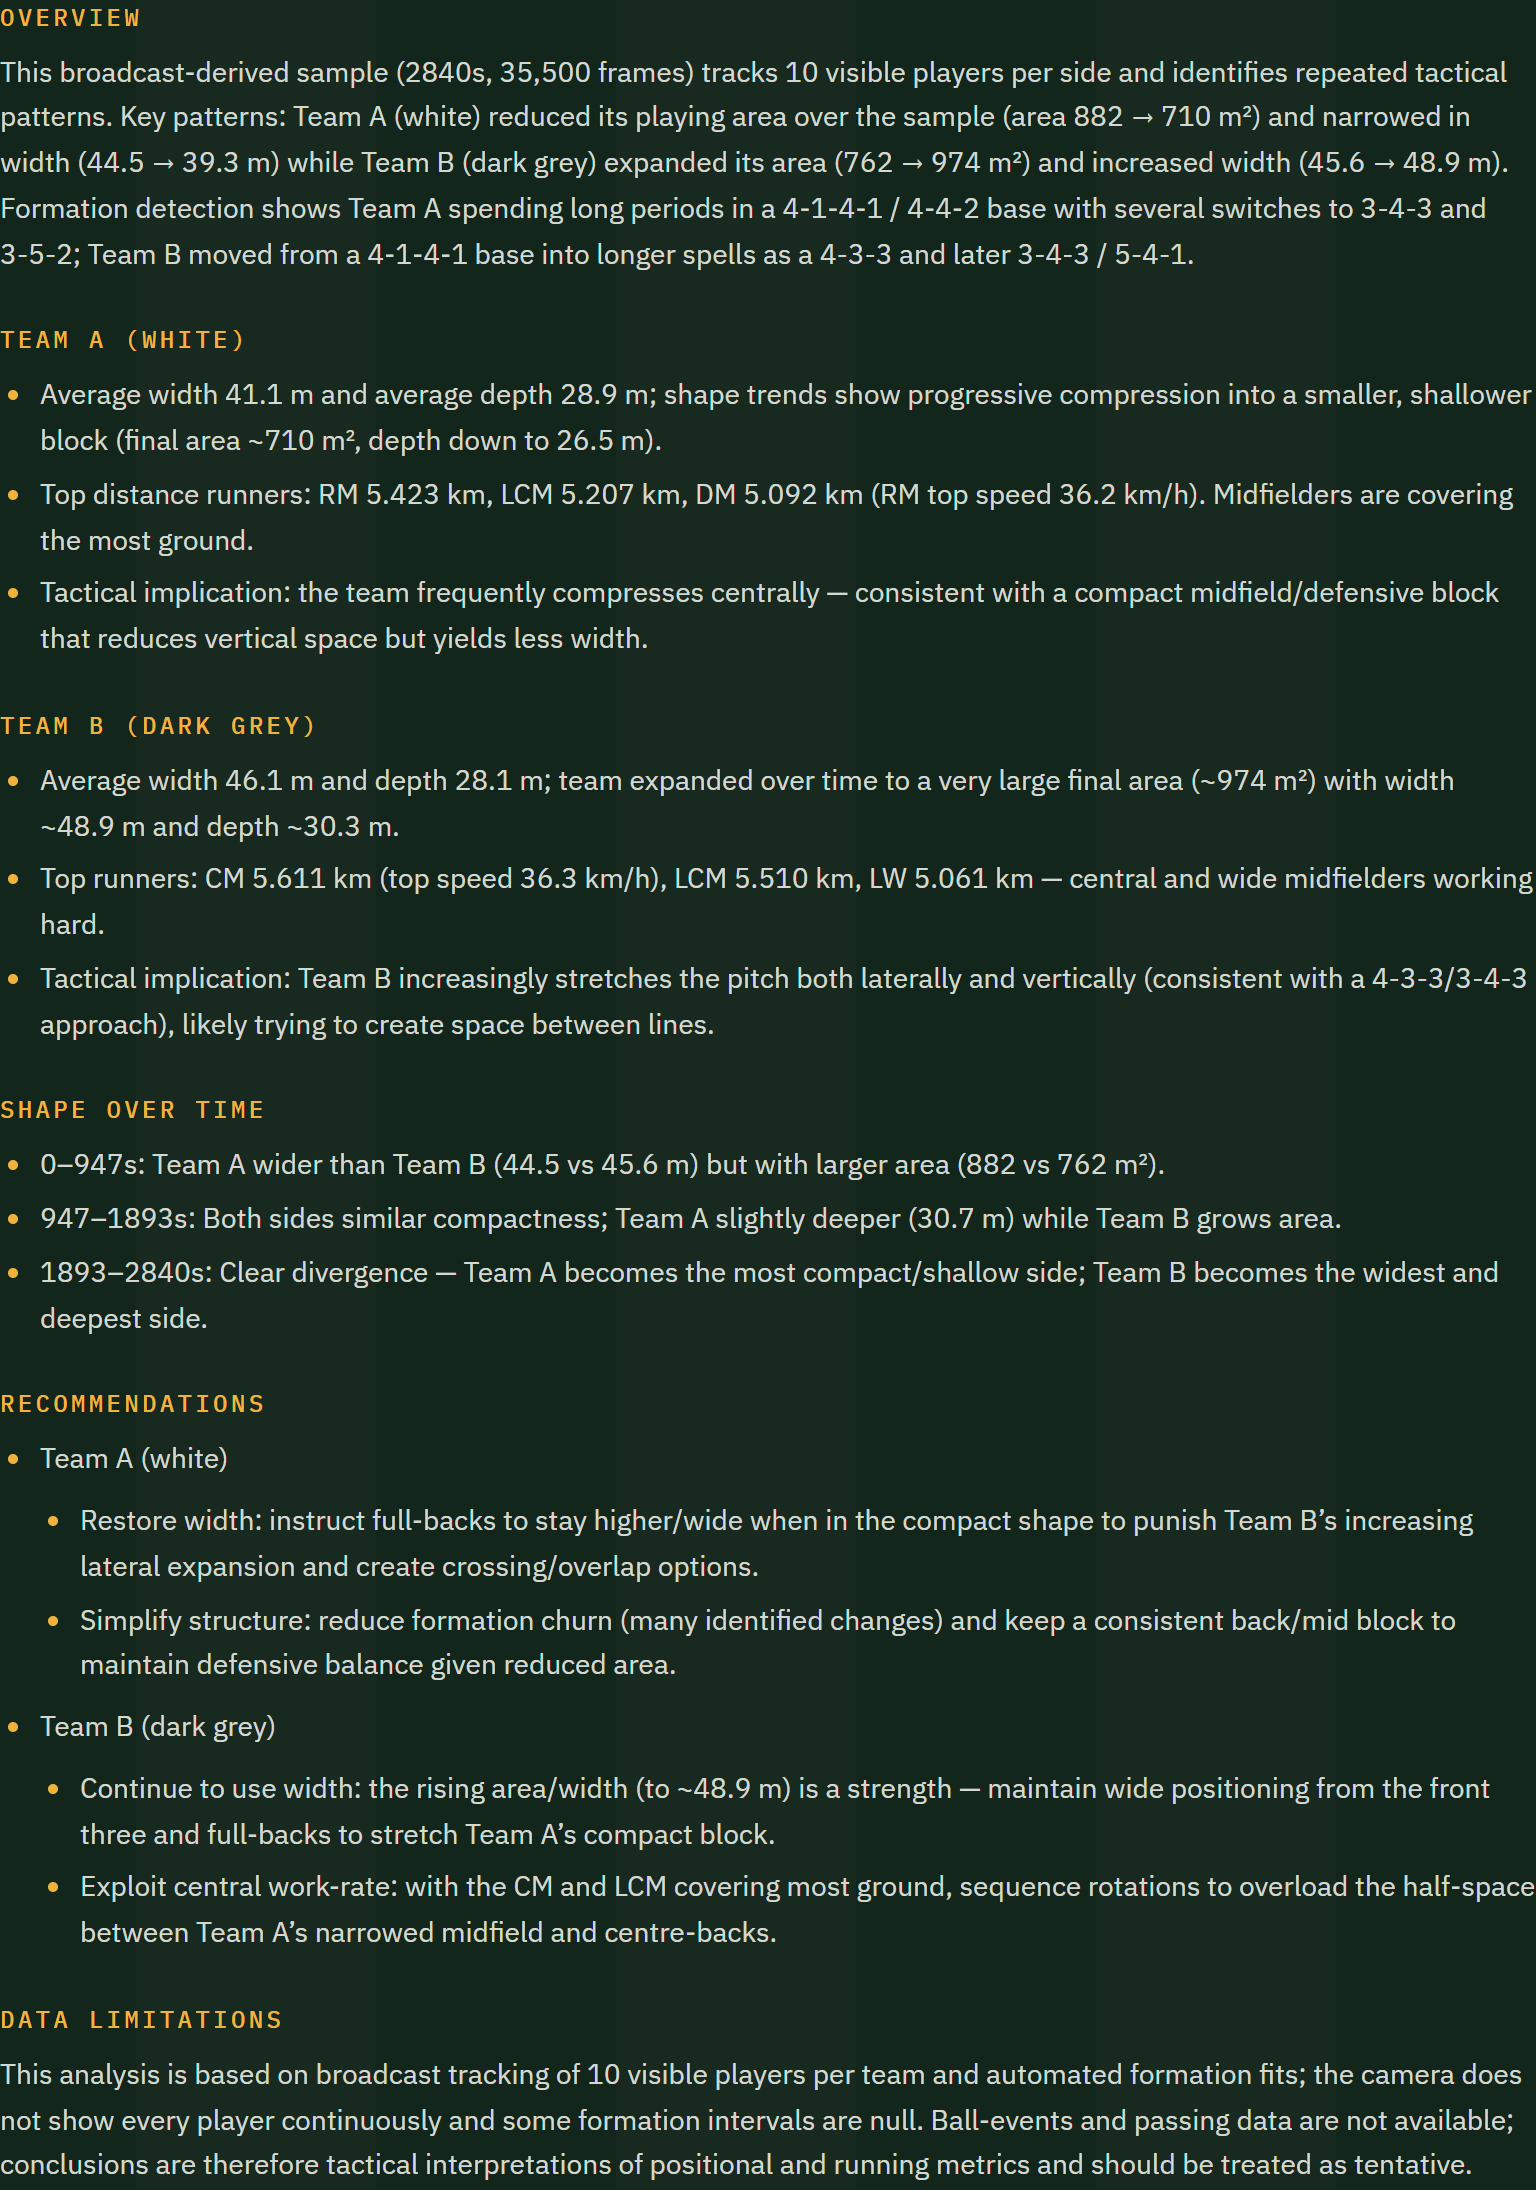
\includegraphics[width=0.82\textwidth]{21_coaching_report}
	\caption{The AI coaching report of the first half}
	\label{fig:report}
\end{figure}

\section{Re-analysing and deleting matches}
\label{sec:reanalyse-delete}

\emph{Re-analyse} (top right of the match page) queues the analysis of the stored video again, in the same mode. It is useful after a software update, after a failure or a cancellation. The previous results stay visible until the new analysis has finished.

\emph{Delete} in a match's row removes the match, its video and all results for good. It asks \emph{Delete?} with \emph{Yes} and \emph{No} first (\autoref{fig:delete}). A match that is being analysed cannot be deleted; it has to be cancelled first, or the user waits until it finishes. A match waiting in the queue can be deleted, and its job is removed from the queue.

\begin{figure}[H]
	\centering
	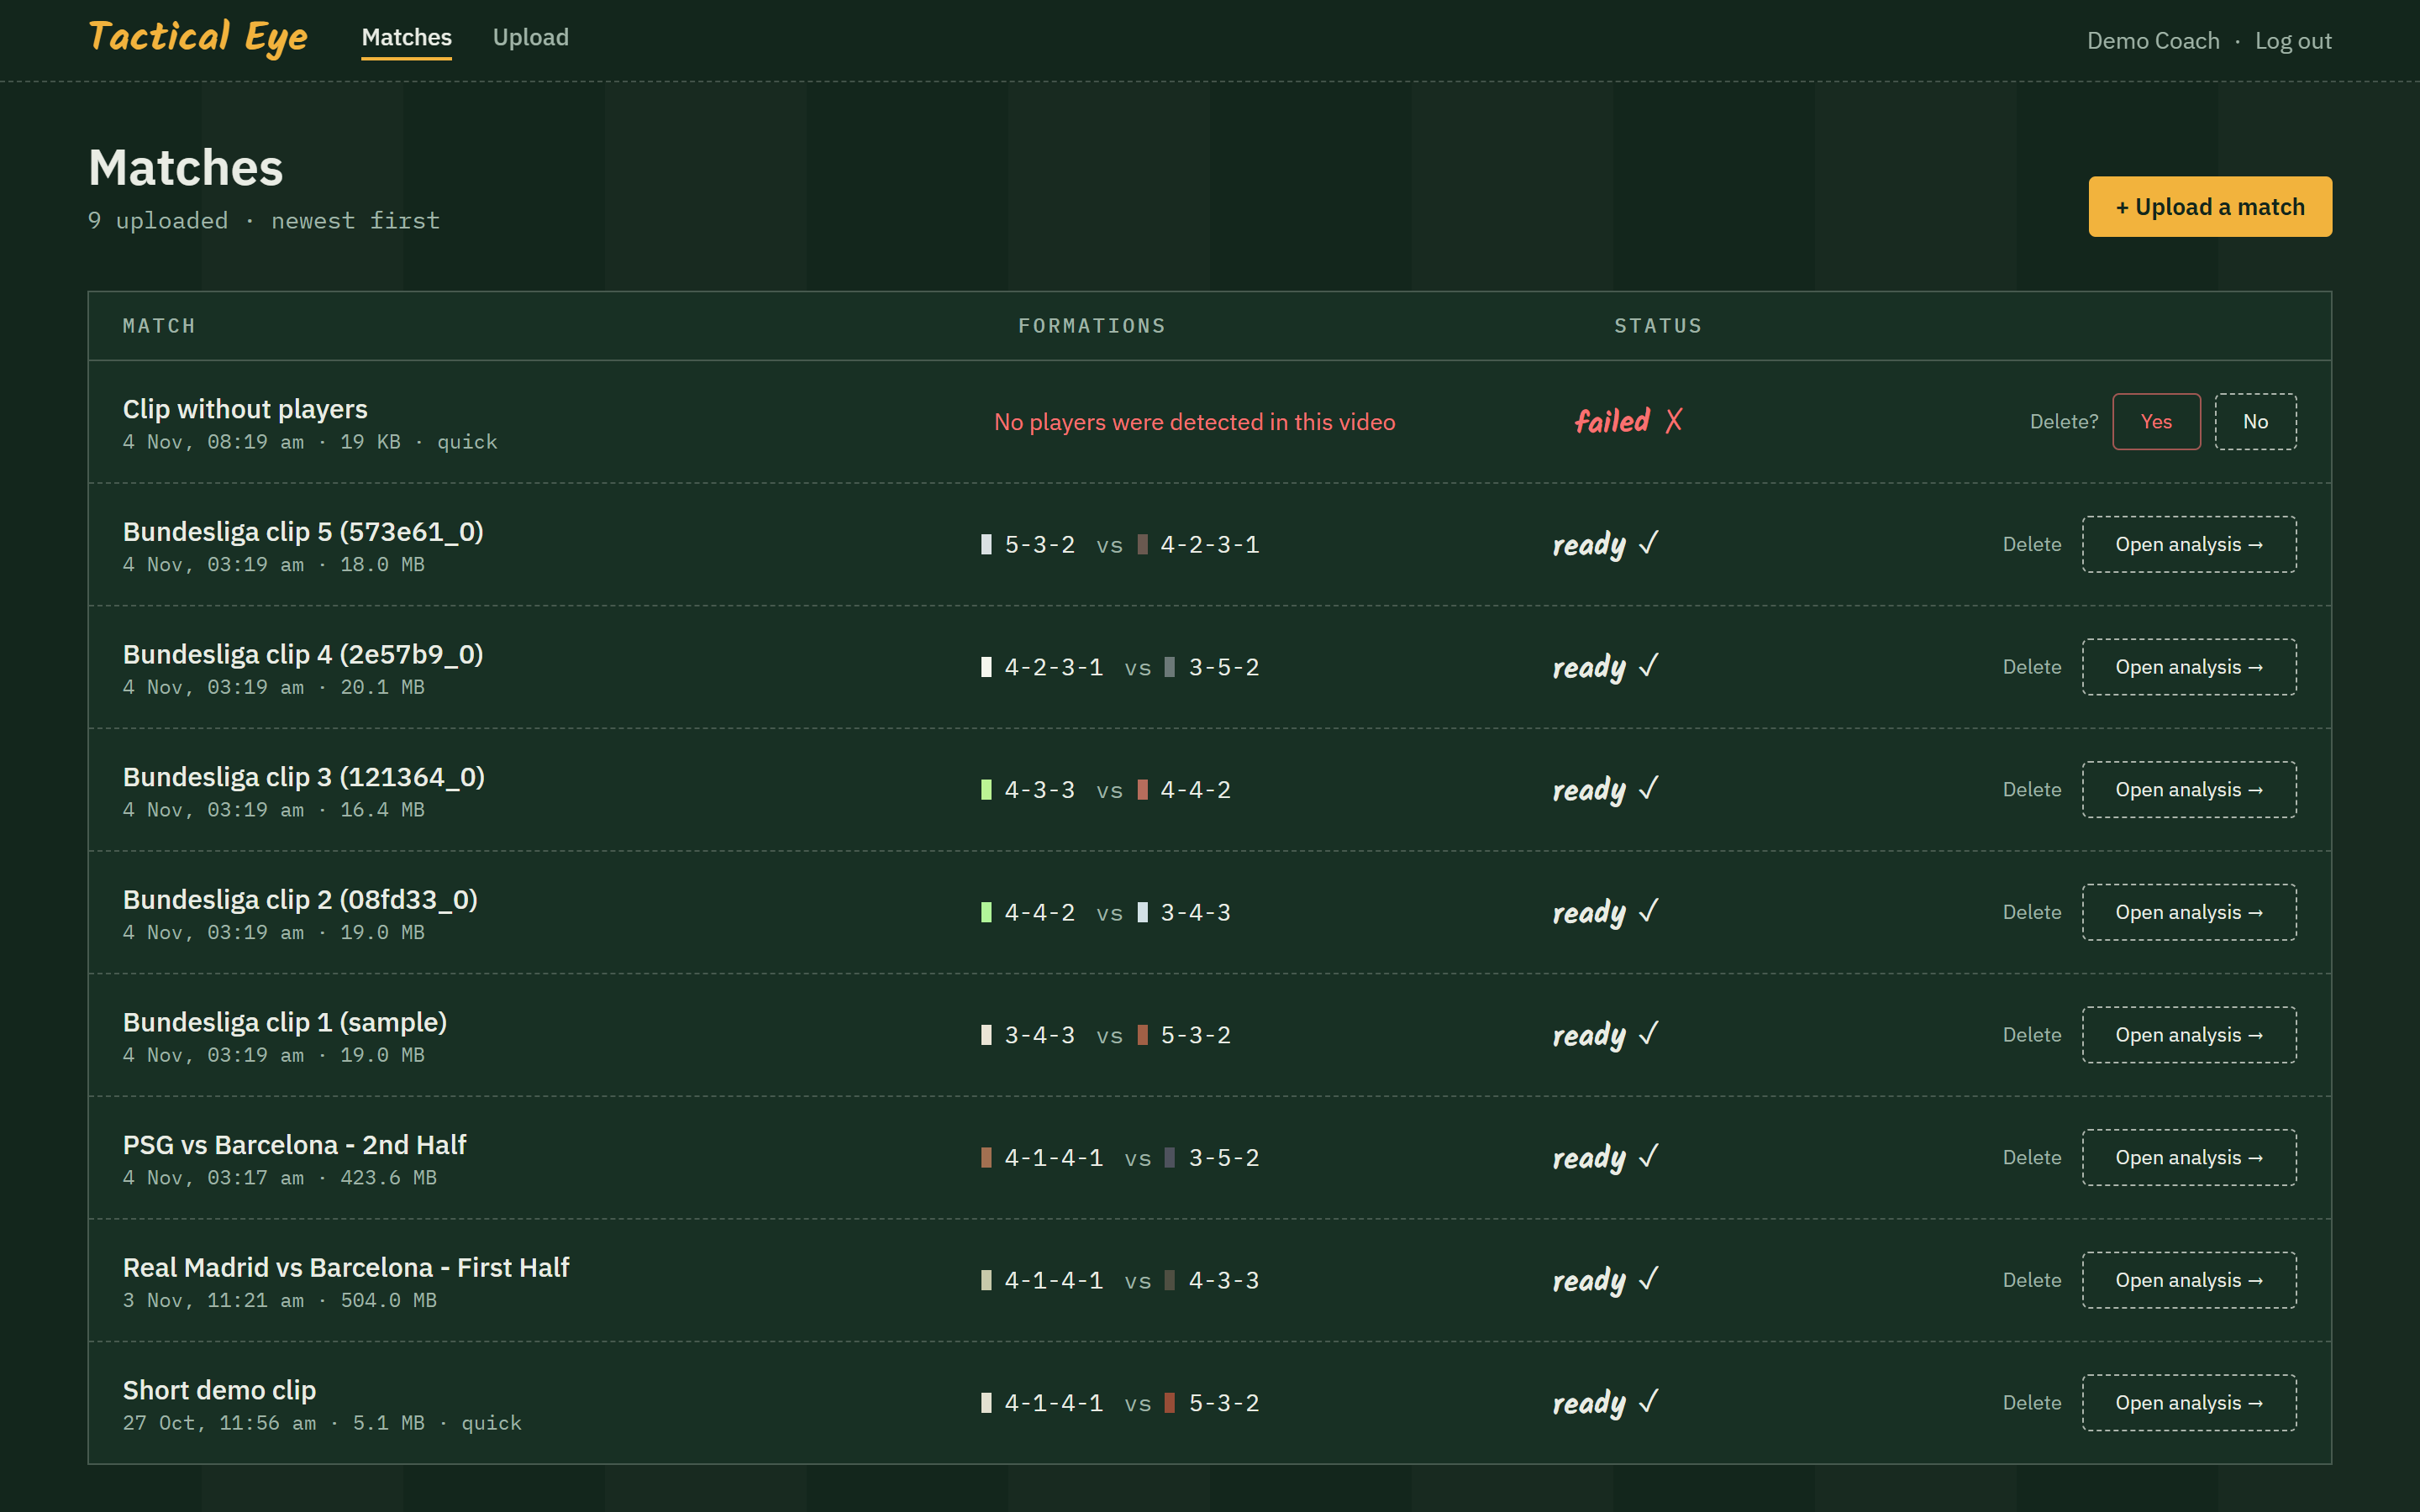
\includegraphics[width=\textwidth]{24_matches_failed_and_delete_confirm}
	\caption{A failed analysis and the delete confirmation}
	\label{fig:delete}
\end{figure}

\section{Messages and troubleshooting}
\label{sec:messages}

\subsection{Error messages}

Errors appear in red next to the action that caused them, or on the row and page of the affected match (\autoref{fig:failed}). \autoref{tab:errors} lists every error message and what to do about it.

\begin{figure}[H]
	\centering
	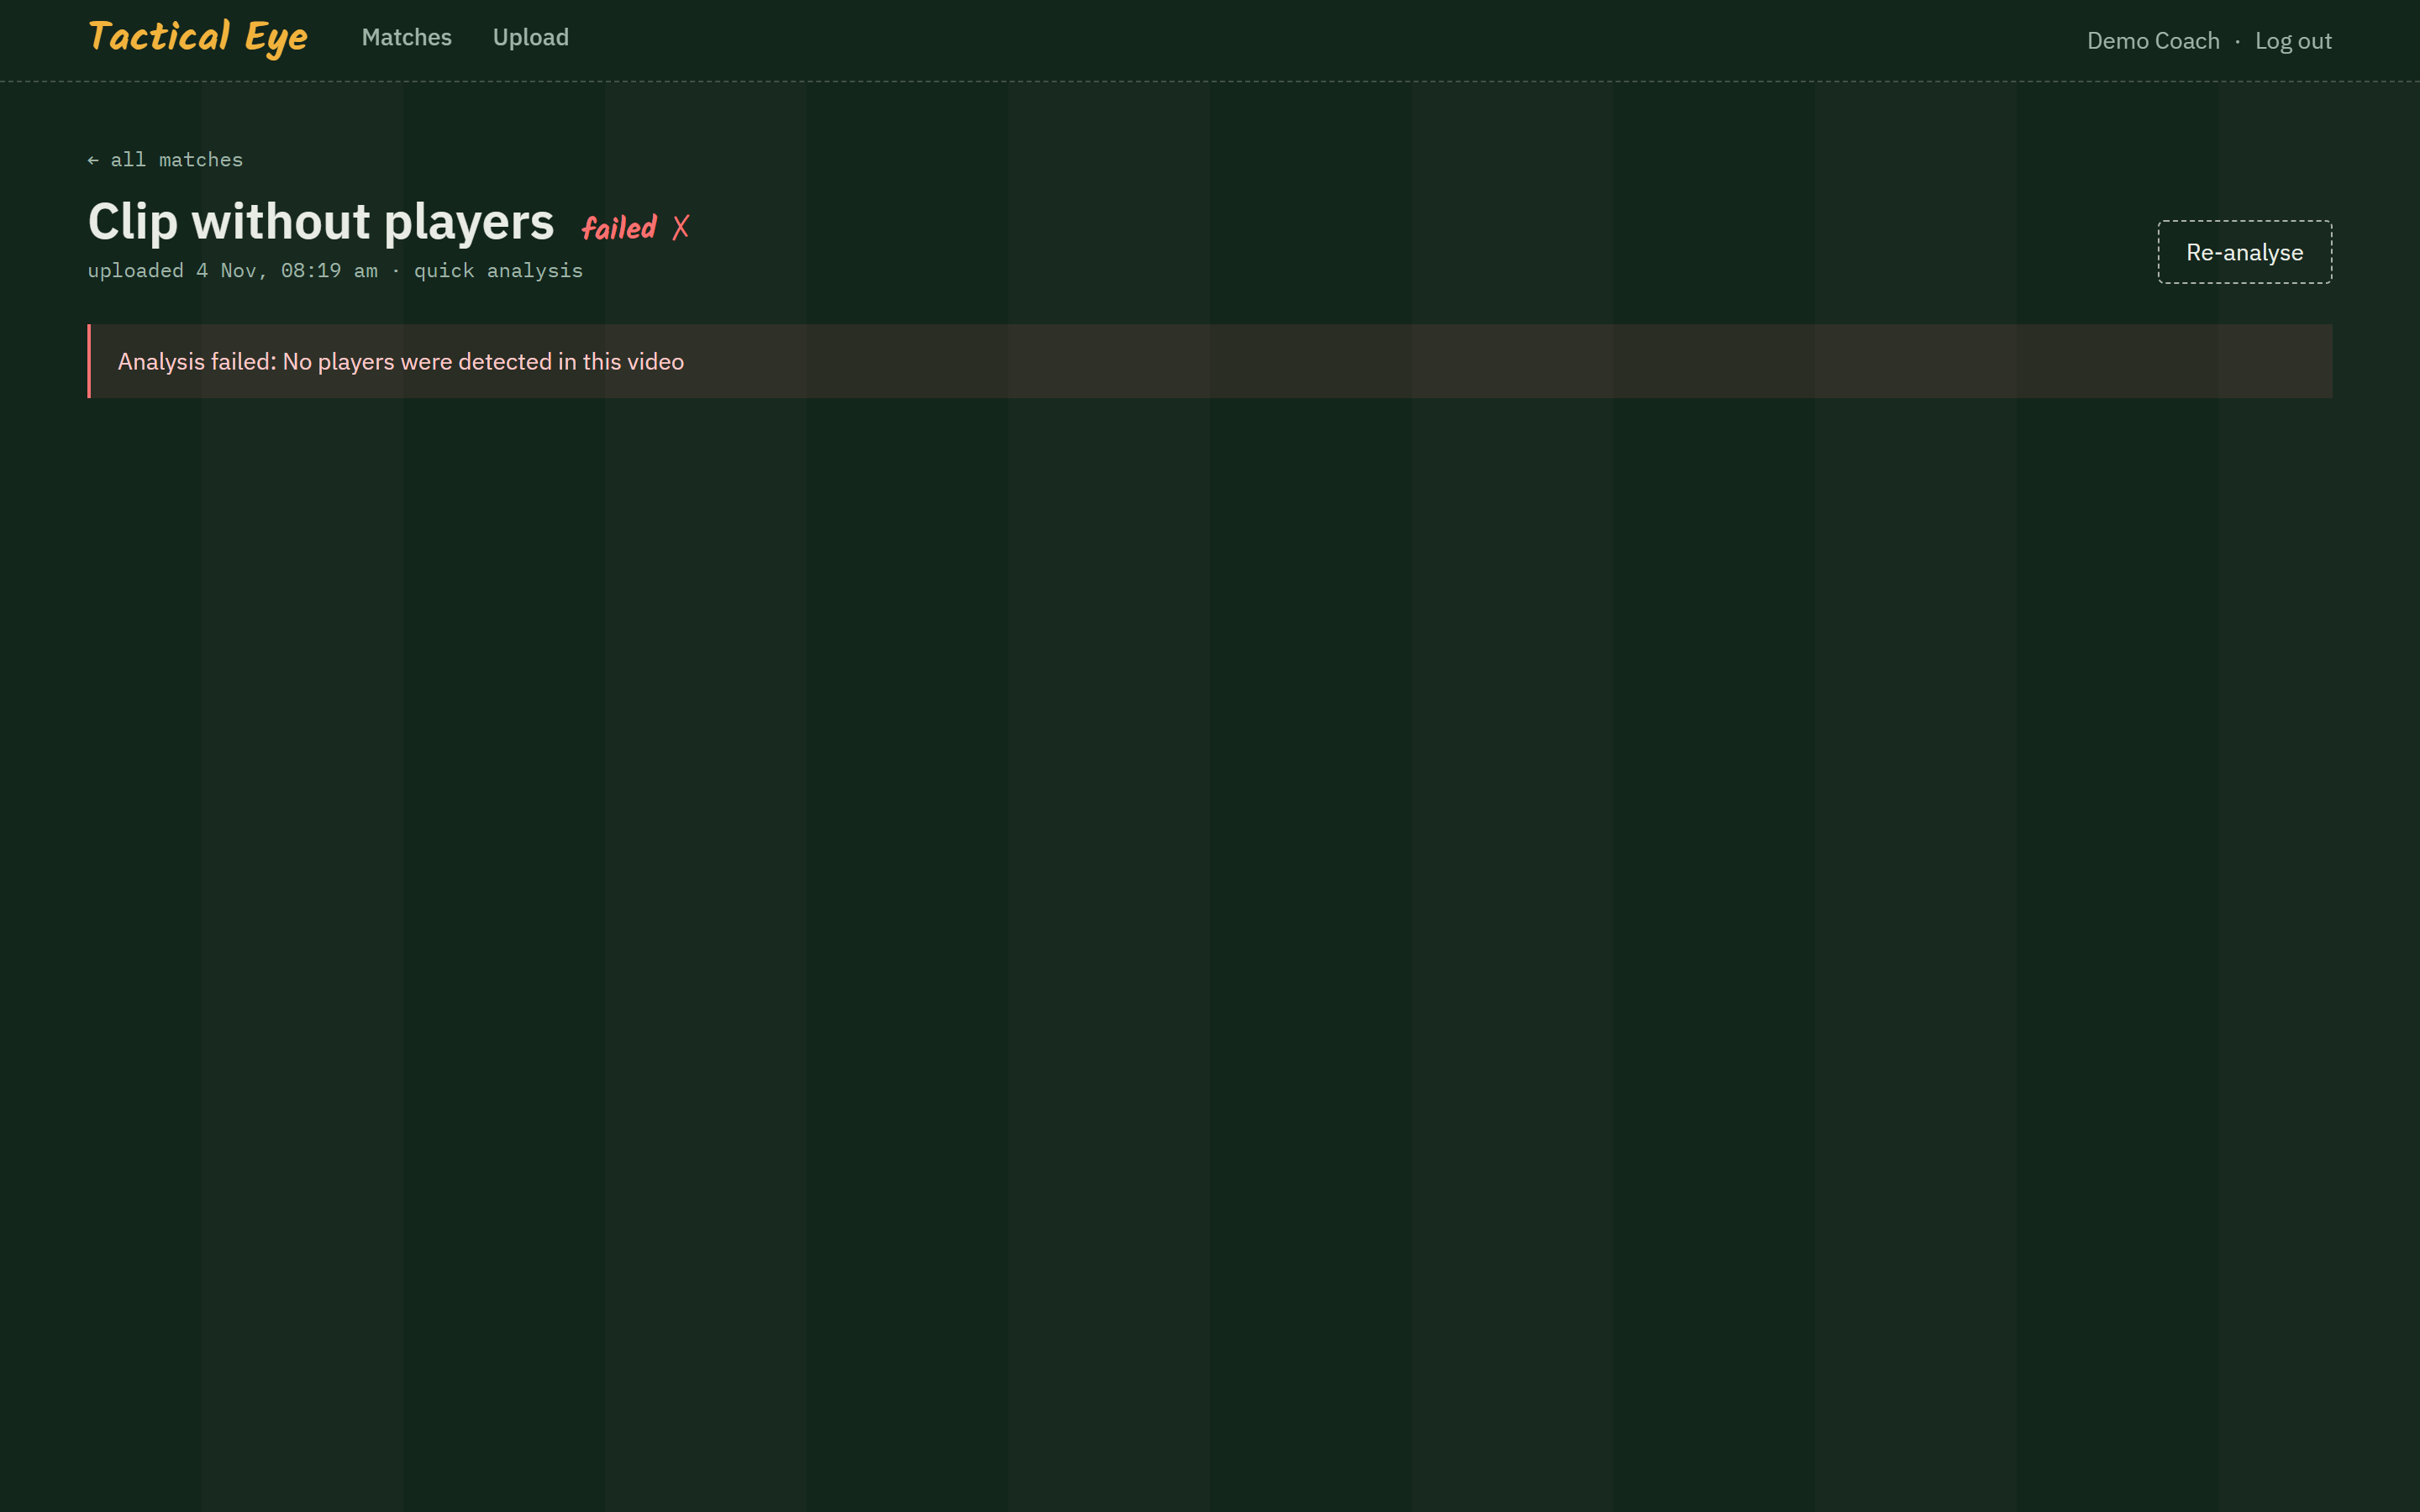
\includegraphics[width=\textwidth]{23_match_failed}
	\caption{The page of a match whose analysis failed}
	\label{fig:failed}
\end{figure}

\begin{longtable}{|p{0.33\textwidth}|p{0.29\textwidth}|p{0.29\textwidth}|}
	\hline
	\textbf{Message} & \textbf{Cause} & \textbf{What to do} \\
	\hline
	\endhead
	Invalid email or password & Wrong e-mail address or password at log-in. & Check both and try again. \\
	\hline
	An account with this email already exists & Registration with an address that is already used. & Log in instead, or use another address. \\
	\hline
	Password must be at least 8 characters & The registration password is too short. & Choose a longer password. \\
	\hline
	Upload a video file (.mp4, .mov, .m4v, .mkv, .webm, .avi) & No file was sent, or its extension or type is not a video. & Choose a file in one of the listed formats. \\
	\hline
	The file is not a valid video & The content is not a video, even though the name ends in a video extension. & Export or download the video again. \\
	\hline
	File is larger than 1024 MB & The upload exceeds the size limit. & Cut or compress the video, or ask the operator to raise \texttt{MAX\_\allowbreak{}UPLOAD\_\allowbreak{}MB}. \\
	\hline
	Network error during upload & The connection was lost during the upload. & Check the connection and upload again. \\
	\hline
	Could not queue the analysis job & The video was stored but the queue (Redis) was unreachable; the match is marked failed. & Operator: check the health address; then use Re-analyse. \\
	\hline
	No players were detected in this video & The analysis found no people, for example the video shows no football or only close-ups. & Use footage from the main broadcast camera. \\
	\hline
	Error, retrying: \dots{} / Retrying after an error & An attempt failed; it is retried once automatically. & Wait. If the second attempt fails too, the match becomes failed. \\
	\hline
	Match not found & The match was deleted, or the link belongs to another user's match. & Return to the match list. \\
	\hline
	This match is already being analysed & Re-analyse while the match is queued or being analysed. & Wait, or cancel the running analysis first. \\
	\hline
	This match is not being analysed & Cancel on a match that has already finished. & Nothing to do; reload the page. \\
	\hline
	This match is being analysed; cancel it first, or delete it when it finishes & Delete during the analysis. & Cancel the analysis, or wait until it finishes. \\
	\hline
	Analysis has not finished yet & Results or a report were requested before the analysis completed. & Wait until the match is ready. \\
	\hline
	The report service is busy; try again in a minute & The AI service limits how many requests it accepts. & Try again after a minute. \\
	\hline
	Could not reach the report service & No connection to Azure OpenAI. & Check the server's internet connection. \\
	\hline
	The Azure OpenAI key is invalid / Azure OpenAI deployment not found & The AI report is set up incorrectly. & Operator: correct the \texttt{AZURE\_\allowbreak{}OPENAI\_\allowbreak{}...} settings and restart the backend. \\
	\hline
	The report was blocked by the Azure content filter / The report came back empty / The report was cut off & The AI service did not return a usable report. & Click Regenerate. \\
	\hline
	Internal server error & An unexpected error on the server; the details go to the server log. & Try again; operator: read \texttt{docker compose logs backend}. \\
	\hline
	\caption{Error messages}
	\label{tab:errors}
\end{longtable}

\subsection{Information and warning messages}

\begin{table}[H]
	\centering
	\begin{tabular}{|p{0.50\textwidth}|p{0.42\textwidth}|}
		\hline
		\textbf{Message} & \textbf{Meaning} \\
		\hline
		No matches yet. & The user has not uploaded anything yet. \\
		\hline
		This page updates live. You can leave it; the analysis keeps running on the server. & Shown during the analysis. \\
		\hline
		Cancel this analysis? You can start it again later with Re-analyse. & Confirmation before cancelling. \\
		\hline
		The analysis was cancelled. Press Re-analyse to start it again. & The analysis was stopped by the user. \\
		\hline
		Click a player on the video or the board to see their movement, heatmap and physical stats. & No player is selected. \\
		\hline
		Paths and heatmaps on the video need a newer analysis of this match. & The match was analysed by an old version without per-frame camera geometry; Re-analyse fixes it. \\
		\hline
		Coaching reports are not configured on this server (Azure OpenAI settings are needed). & The operator has not enabled the AI report. \\
		\hline
		Analysing the statistics (about 10-30 seconds) & A report is being written. \\
		\hline
	\end{tabular}
	\caption{Information and warning messages}
	\label{tab:info-messages}
\end{table}

\subsection{Frequently asked questions}

\paragraph{The analysis is very slow.} On a CPU the analysis takes many times the length of the video. Quick mode helps for previews; for full halves, the cloud GPU service is the practical choice (\autoref{sec:cloud-gpu}).

\paragraph{The match stays queued.} No worker is running, or another match is being analysed first. The health address (\texttt{/api/health}) shows the number of workers; if it is 0, \texttt{docker compose --profile app up -d worker} starts the worker.

\paragraph{The labels change from one player to another.} Labels follow positions. When two players swap sides, their labels swap too, and a player who has only just come into view may have no label for a few seconds.

\paragraph{The formation looks wrong.} A formation needs at least 8 outfield players of the team to be visible in a 5-second window. When the runner-up is close, the team's shape really is between two formations.

\paragraph{The video does not play.} Every upload is converted into a format browsers can play. If the browser still cannot play it, an update of the browser usually helps; Chrome and Edge are recommended.

\subsection{Security and privacy}

Passwords are never stored, only a salted bcrypt hash of them, and the session cookie cannot be read by scripts on the page. Users can only see, change, cancel and delete their own matches; links to other users' matches answer \emph{Match not found}. Uploaded files are checked for real video content and stored under random names. The AI report service receives only the computed statistics, never the video or personal data. When the platform is reachable from the internet, the operator should serve it over HTTPS, for example behind a reverse proxy with a certificate, and keep \texttt{COOKIE\_\allowbreak{}SECURE} at its default.

\cleardoublepage

\chapter{Developer documentation}
\label{ch:developer}

This chapter describes the design and implementation of Tactical Eye for developers who want to maintain or extend it. The source code has one folder per service: \texttt{frontend/} (React dashboard), \texttt{backend/} (Node.js API) and \texttt{worker/} (Python AI worker), next to \texttt{docker-compose.\allowbreak{}yml}, the CI/CD workflow and the tests.

\section{Requirements}

\subsection{Functional requirements}

\begin{longtable}{|p{0.06\textwidth}|p{0.60\textwidth}|p{0.25\textwidth}|}
	\hline
	\textbf{ID} & \textbf{Requirement} & \textbf{Realised in} \\
	\hline
	\endhead
	F1 & Users can register with name, e-mail and password, log in and log out; a session lasts 7 days. & \texttt{routes/auth.\allowbreak{}ts}, \texttt{AuthPage} \\
	\hline
	F2 & Users can upload a match video (MP4, MOV, M4V, MKV, WebM, AVI, up to 1\,GB) with a title and an analysis mode and see the upload progress. & \texttt{routes/matches.\allowbreak{}ts}, \texttt{UploadPage} \\
	\hline
	F3 & Uploads are analysed asynchronously by workers through a job queue; the web request returns at once. & \texttt{queue.\allowbreak{}ts}, \texttt{worker.\allowbreak{}py} \\
	\hline
	F4 & The progress of each analysis (percentage and step) appears live, without reloading. & Socket.IO, \texttt{useMatchUpdates} \\
	\hline
	F5 & Players, goalkeepers, referees and the ball are detected and tracked. & \texttt{detector.\allowbreak{}py}, \texttt{tracker.\allowbreak{}py} \\
	\hline
	F6 & Positions are converted from image pixels to pitch coordinates in metres. & \texttt{homography.\allowbreak{}py} \\
	\hline
	F7 & People standing off the pitch and objects that only look like the ball are removed. & \texttt{cleanup.\allowbreak{}py} \\
	\hline
	F8 & Players are split into two teams; goalkeepers join their team; referees are recognised, also when the detector calls them players. & \texttt{clustering.\allowbreak{}py} \\
	\hline
	F9 & Each team's formation is recognised over time and every player gets a position label (LB, CB, ST\dots). & \texttt{clustering.\allowbreak{}py}, \texttt{positions.\allowbreak{}py} \\
	\hline
	F10 & Compactness, width, depth, distances, speeds and heatmaps are computed for teams, positions and the ball. & \texttt{metrics.\allowbreak{}py} \\
	\hline
	F11 & Results are drawn on the video (players, paths, team shape, ball, heatmaps), in sync frame by frame, also in full screen. & \texttt{VideoAnalysis}, \texttt{draw.\allowbreak{}ts} \\
	\hline
	F12 & A 2D tactical board shows the same moment from above with the current formations. & \texttt{drawBoard}, \texttt{VideoAnalysis} \\
	\hline
	F13 & Clicking a player shows the heatmap, path, distance, time visible and speeds of their position. & \texttt{PlayerPanel} \\
	\hline
	F14 & A language model writes a coaching report from the statistics; the report is stored. & \texttt{report.\allowbreak{}ts}, \texttt{CoachingReport} \\
	\hline
	F15 & Users can list, re-analyse, cancel and delete their own matches, and cannot reach other users' matches. & \texttt{routes/matches.\allowbreak{}ts} \\
	\hline
	F16 & Analysis can run on a remote GPU service, with automatic fallback to local analysis. & \texttt{remote.\allowbreak{}py}, \texttt{gpu\_\allowbreak{}server.\allowbreak{}py} \\
	\hline
	F17 & Videos of a full half (about 48 minutes, up to 1\,GB, any codec, 25 or 50\,fps) can be analysed. & \texttt{pipeline.\allowbreak{}py}, \texttt{remote.\allowbreak{}py} \\
	\hline
	\caption{Functional requirements}
	\label{tab:functional}
\end{longtable}

\subsection{Non-functional requirements}

\begin{table}[H]
	\centering
	\small
	\begin{tabular}{|p{0.06\textwidth}|p{0.18\textwidth}|p{0.67\textwidth}|}
		\hline
		\textbf{ID} & \textbf{Quality} & \textbf{Requirement} \\
		\hline
		N1 & Responsiveness & No web request waits for an analysis; heavy work runs in workers, and the dashboard stays usable meanwhile. \\
		\hline
		N2 & Scalability & Analysis capacity grows by adding workers or a GPU, without changes to the API or the dashboard. \\
		\hline
		N3 & Reliability & A failed or crashed analysis is retried; partial results are never shown; a lost GPU service falls back to local analysis; a job handed out twice is not analysed twice. \\
		\hline
		N4 & Security & Hashed passwords, script-proof session cookies, validated uploads, users isolated from each other, secrets kept out of the repository. \\
		\hline
		N5 & Deployability & One command starts the platform; every service has a container image, built and published automatically after the tests pass. \\
		\hline
		N6 & Maintainability & Typed code (TypeScript, Python type hints), validation of all external input, and automated unit, API and system tests on every change. \\
		\hline
		N7 & Usability & Overlays are synchronised to the exact video frame; the dashboard works in current browsers and adapts to smaller screens. \\
		\hline
		N8 & Efficiency & Long videos are streamed and never held in memory; the AI models are loaded once per worker process; memory stays below 5\,GB for a full half. \\
		\hline
	\end{tabular}
	\caption{Non-functional requirements}
	\label{tab:nonfunctional}
\end{table}

\subsection{Use cases}

\autoref{fig:usecase} shows the actors and their use cases. The registered user is the main actor. The AI worker is a system actor that drives the analysis and the progress updates, and the operator deploys and configures the platform outside the dashboard. \autoref{tab:stories} gives the main use cases as user stories.

\begin{figure}[H]
	\centering
	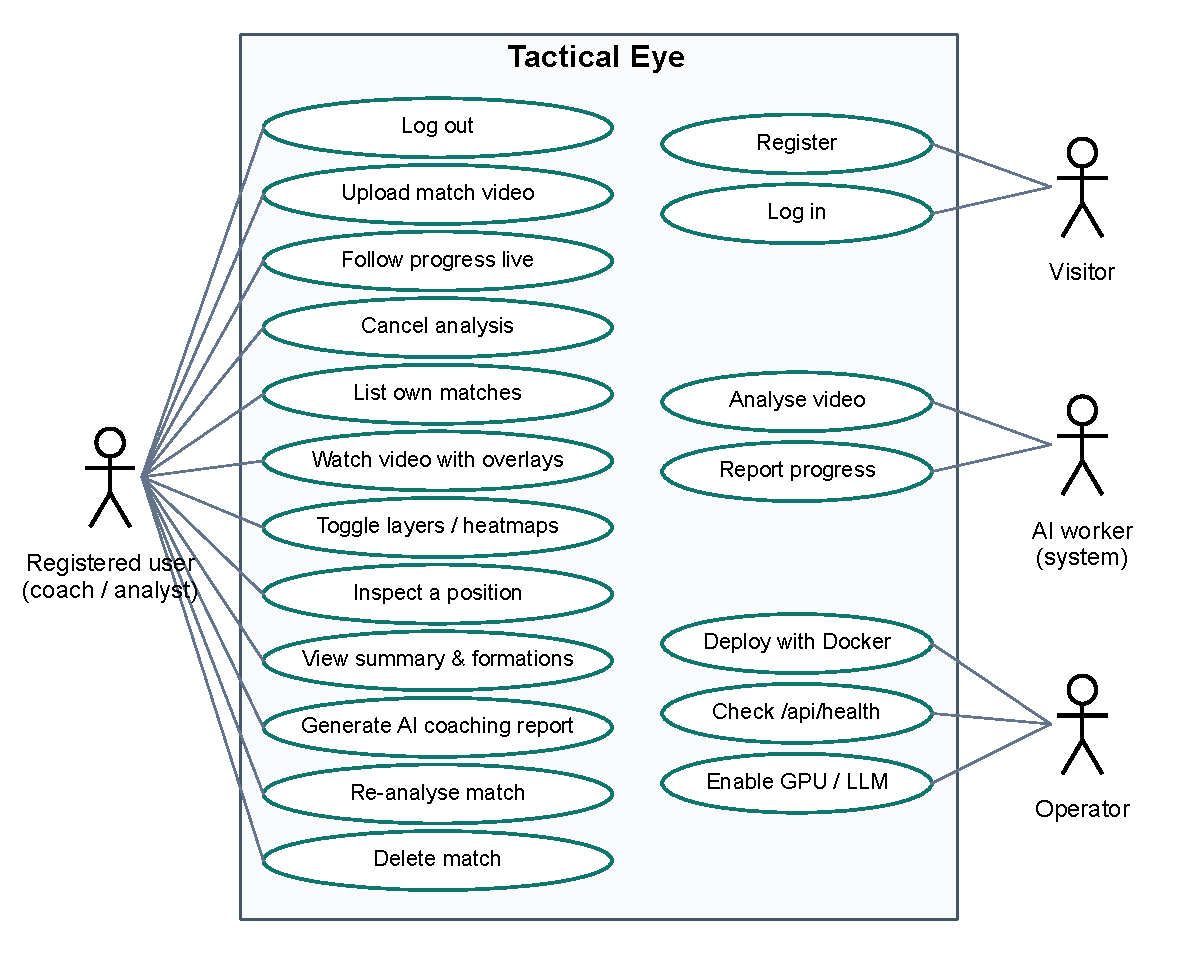
\includegraphics[width=\textwidth]{usecase}
	\caption{Use case diagram}
	\label{fig:usecase}
\end{figure}

\begin{longtable}{|p{0.18\textwidth}|p{0.74\textwidth}|}
	\hline
	\textbf{Use case} & \textbf{User story} \\
	\hline
	\endhead
	Upload a match & \emph{Given} a logged-in user with a video, \emph{when} they choose the file, a title and a mode and press \emph{Upload and analyse}, \emph{then} the video is stored, a queued match appears and its page opens. \\
	\hline
	Follow progress & \emph{Given} a match being analysed, \emph{when} the worker finishes a step, \emph{then} the progress bar and step label update on every open page of that user within a second. \\
	\hline
	Cancel & \emph{Given} a queued or running analysis, \emph{when} the user confirms \emph{Cancel analysis}, \emph{then} a queued job is removed at once and a running one stops within seconds, and the match shows as cancelled, or keeps its earlier results if it was a re-analysis. \\
	\hline
	Watch the analysis & \emph{Given} a finished match, \emph{when} the user plays the video, \emph{then} labels, paths and shapes stay on the players in every frame, also while the camera pans, and the board shows the same moment. \\
	\hline
	Inspect a position & \emph{Given} the analysis page, \emph{when} the user clicks a player, \emph{then} the player is highlighted and the heatmap, path, distance and speeds of their position are shown. \\
	\hline
	Generate a report & \emph{Given} a finished match and a configured model, \emph{when} the user presses \emph{Generate report}, \emph{then} a Markdown report based only on the statistics is shown and stored. \\
	\hline
	Retry after failure & \emph{Given} a worker that crashes during a job, \emph{when} its job lock expires, \emph{then} the job goes to a worker again; after a second failure the match is shown as failed with the reason. \\
	\hline
	\caption{User stories of the main use cases}
	\label{tab:stories}
\end{longtable}

\section{System architecture}

\subsection{Overview}

Tactical Eye is a distributed system with an asynchronous job queue (\autoref{fig:architecture}). It separates three parts with very different resource needs. The presentation tier is the React single-page application in the browser, which renders the dashboard and the overlays. The application tier is the Node.js API, which handles many short requests (log-in, uploads, lists, video streaming, live updates) and must stay responsive. The processing tier is the Python AI workers, which run long CPU- or GPU-bound analyses, one at a time.

\begin{figure}[H]
	\centering
	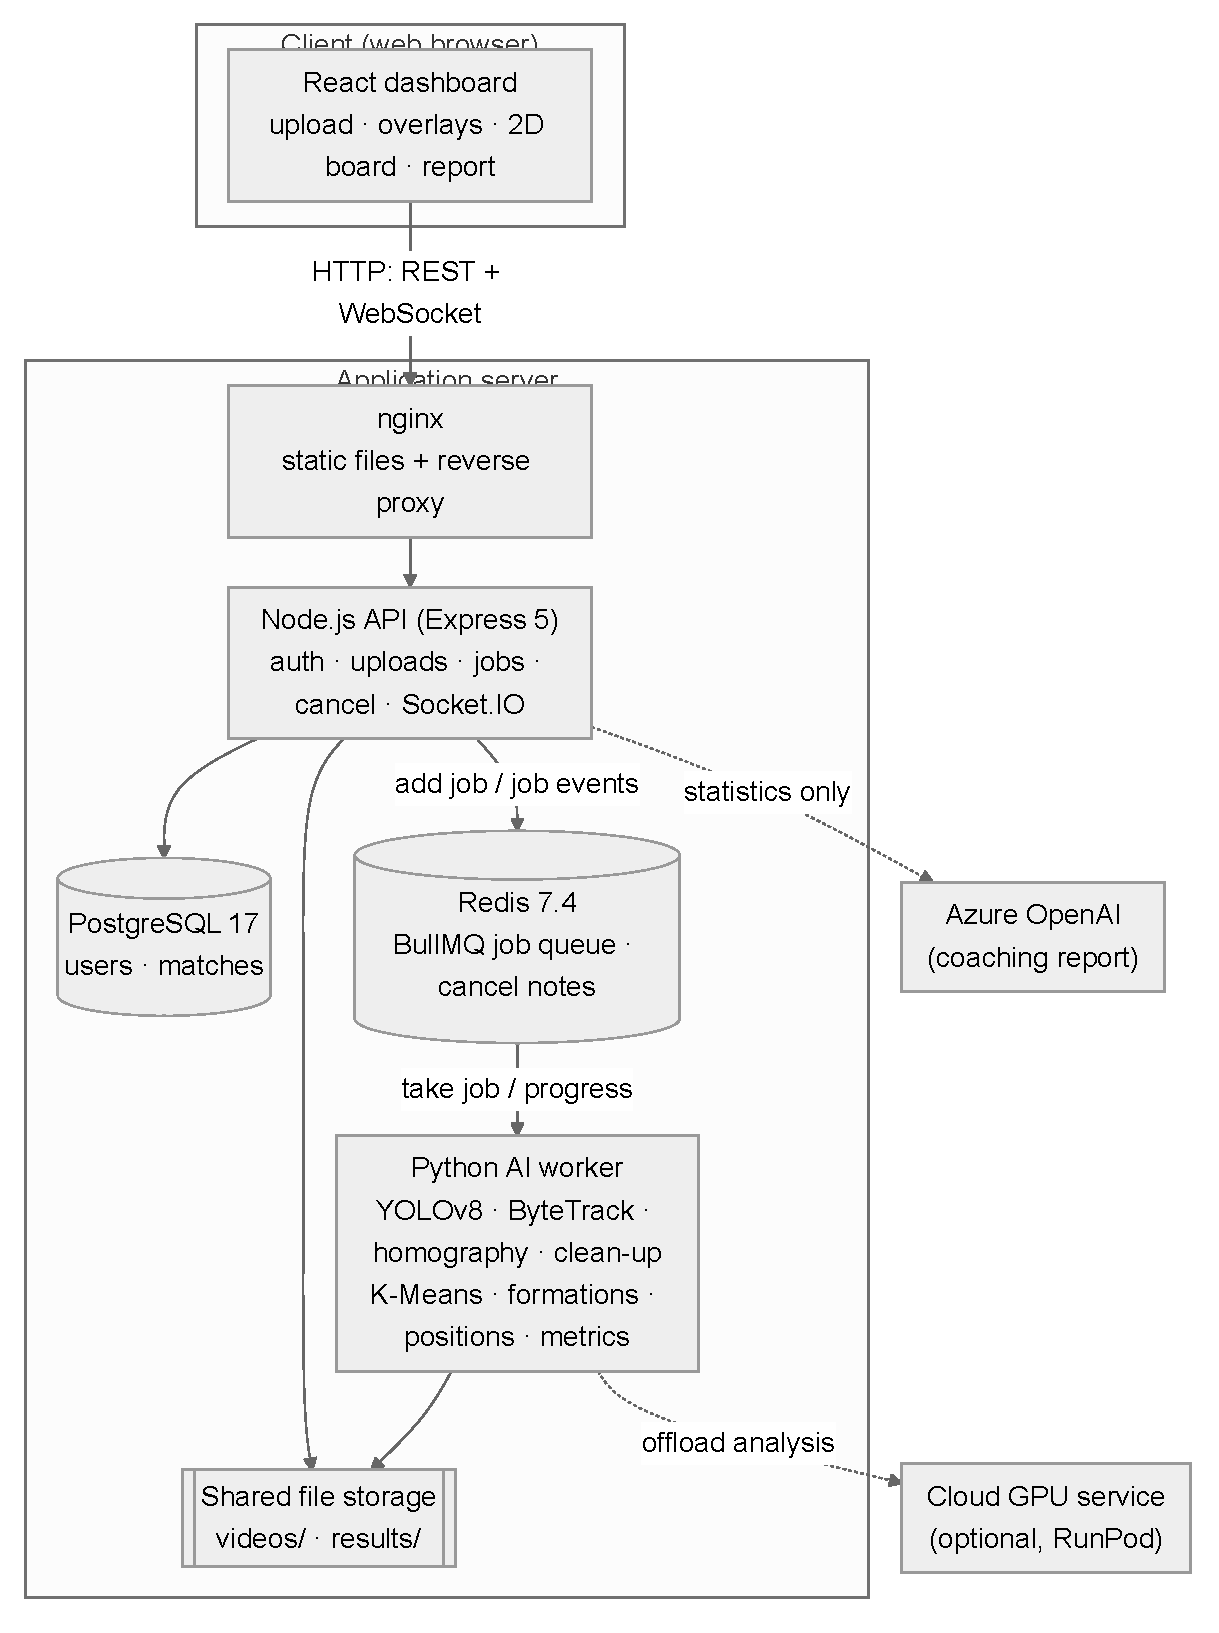
\includegraphics[width=0.8\textwidth]{architecture}
	\caption{Components and communication paths}
	\label{fig:architecture}
\end{figure}

The tiers talk through narrow interfaces: REST and a WebSocket between browser and API, a Redis-backed BullMQ queue~\cite{bullmq} between API and workers, a shared folder for videos and results, and the PostgreSQL database~\cite{postgres}, which only the API uses.

The central decision was that the API never runs an analysis itself. An upload creates a database row and a queue job and returns immediately, and workers pull jobs whenever they are free. I made this choice after the first prototype ran the pipeline inside the request handler: a 30-second clip kept the request open for 25 minutes, the browser gave up long before that, and a crash took the API down with it. With the queue, the API can serve many users while one worker spends an hour on a full half, workers can be added or removed without the API noticing, and jobs survive restarts because Redis stores them.

Progress flows the other way. The worker reports progress to the queue, the queue emits events, and the API, which listens to these events, updates the database and pushes the change to the browser over Socket.IO~\cite{socketio}. The browser never polls.

\subsection{Technology choices}

\autoref{tab:technologies} lists the technologies and their versions. The reasons behind the larger choices matter more than the list, so they follow the table.

\begin{longtable}{|p{0.13\textwidth}|p{0.33\textwidth}|p{0.45\textwidth}|}
	\hline
	\textbf{Layer} & \textbf{Technology} & \textbf{Purpose} \\
	\hline
	\endhead
	Frontend & React 19, TypeScript 6 & Component-based user interface~\cite{react}. \\
	\cline{2-3}
	& Vite 8, Vitest 4 & Development server, production bundler and unit tests~\cite{vite,vitest}. \\
	\cline{2-3}
	& React Router 8, Tailwind CSS 4 & Client-side routing; utility-first styling~\cite{tailwind}. \\
	\cline{2-3}
	& Socket.IO client 4.8, react-markdown 10 & Live updates; rendering the coaching report. \\
	\cline{2-3}
	& HTML5 Canvas, \texttt{request\allowbreak{}Video\allowbreak{}Frame\allowbreak{}Callback}, Fullscreen API & Frame-synchronised drawing and full-screen view~\cite{rvfc}. \\
	\hline
	Backend & Node.js 24, Express 5, TypeScript 6 & REST API~\cite{express}; Express 5 passes errors of async handlers to the error middleware. \\
	\cline{2-3}
	& Prisma 7, PostgreSQL 17 & Typed database access and migrations~\cite{prisma,postgres}. \\
	\cline{2-3}
	& BullMQ 6, Redis 7.4 & Job queue, queue events and the cancel notes~\cite{bullmq,redis}. \\
	\cline{2-3}
	& Socket.IO 4.8, Zod 4 & WebSocket server; validation of requests and settings. \\
	\cline{2-3}
	& Multer 2, bcryptjs 3, jsonwebtoken 9 & Uploads, password hashing, session tokens~\cite{jwt}. \\
	\cline{2-3}
	& openai 6 (\texttt{AzureOpenAI} client) & Coaching reports~\cite{azureopenai}. \\
	\cline{2-3}
	& Vitest 4, SuperTest 7 & API tests against a real test database~\cite{vitest,supertest}. \\
	\hline
	AI worker & Python 3.12 & Worker language. \\
	\cline{2-3}
	& Ultralytics 8.4 (YOLOv8), PyTorch 2.14 & Object and keypoint detection~\cite{yolov8,pytorch}. \\
	\cline{2-3}
	& trackers 2.6 (ByteTrack), supervision 0.31 & Multi-object tracking and detection utilities~\cite{bytetrack,supervision}. \\
	\cline{2-3}
	& OpenCV 5, NumPy 2.5, pandas 3, SciPy 1.18, scikit-learn 1.9 & Homography, colour spaces, data processing, Hungarian algorithm, convex hulls, K-Means~\cite{opencv,sklearn}. \\
	\cline{2-3}
	& PyAV 19 (libx264, dav1d) & Reading any codec, writing the H.264 playback copy~\cite{pyav}. \\
	\cline{2-3}
	& bullmq 3.4 (Python), redis 8, psutil & Queue consumer compatible with Node.js BullMQ; cancel notes; memory measurement. \\
	\cline{2-3}
	& FastAPI, uvicorn, httpx, pytest & Remote GPU service and its client; unit tests~\cite{pytest}. \\
	\hline
	Operations & Docker, Docker Compose, nginx 1.27 & Containers, orchestration, reverse proxy~\cite{docker}. \\
	\cline{2-3}
	& GitHub Actions, GitHub Container Registry & CI/CD pipeline and image registry~\cite{ghactions}. \\
	\cline{2-3}
	& Azure OpenAI (\texttt{gpt-5-mini}), RunPod (NVIDIA L4) & External language model and GPU~\cite{runpod}. \\
	\hline
	\caption{Technologies and versions}
	\label{tab:technologies}
\end{longtable}

TypeScript runs on both the frontend and the API, so the shapes of shared data (a match, the results file) are written once and checked by the compiler on both sides. The worker is in Python because the computer vision ecosystem is: PyTorch, Ultralytics, OpenCV and pandas have no comparable counterparts in Node.js. Two languages need a queue that both understand. Celery would have tied the queue to Python and RabbitMQ would have added another server; BullMQ has a Node.js and a Python implementation that share the same Redis data structures, so the API adds jobs in TypeScript and the worker takes them in Python.

PostgreSQL won over MongoDB because the data is relational (users own matches, and every query filters by owner) and because its JSON column still lets me store the loosely structured match summary without a schema for every number. I chose Prisma over writing SQL by hand because it generates a typed client and a migration file for every schema change; the \texttt{CANCELLED} status, for example, became a one-line schema change and a generated \texttt{ALTER TYPE} migration.

For detection I used YOLOv8 with weights that Roboflow trained on broadcast football~\cite{roboflowsports}. Training my own model was not realistic: it needs thousands of annotated frames and GPU time I did not have, while these weights already know the classes ball, goalkeeper, player and referee. ByteTrack~\cite{bytetrack} was chosen because it keeps low-confidence detections in a second matching round, which is exactly what happens to partly hidden players in crowded penalty areas.

Drawing the analysis in the browser instead of burning it into a new video was a deliberate choice as well. A rendered video would have been simpler to show, but every layer combination would need its own video, nothing could be clicked, and a full half would mean rendering another gigabyte. Drawing on a canvas from the results file lets the user switch layers, select players and step through frames, at the cost of the synchronisation work described in \autoref{sec:overlay-sync}.

\subsection{Layers inside the services}

Each service is layered as well. In the frontend, pages (one per route) compose reusable components; all server communication goes through one API module (\texttt{api.\allowbreak{}ts}) and one WebSocket hook (\texttt{useMatchUpdates}); and the pure analysis modules (\texttt{timeline.\allowbreak{}ts}, \texttt{geometry.\allowbreak{}ts}, \texttt{draw.\allowbreak{}ts}) contain the overlay logic with no dependency on React, which also makes them easy to unit-test. In the backend, routes handle HTTP and validate input, then call service modules (\texttt{queue.\allowbreak{}ts}, \texttt{storage.\allowbreak{}ts}, \texttt{report.\allowbreak{}ts}, \texttt{colours.\allowbreak{}ts}, \texttt{auth.\allowbreak{}ts}), which use the Prisma client in \texttt{db.\allowbreak{}ts}. \texttt{config.\allowbreak{}ts} validates all settings at start-up. In the worker, the queue adapter (\texttt{worker.\allowbreak{}py}) knows nothing about computer vision; it calls the pipeline orchestrator (\texttt{pipeline.\allowbreak{}py}), which chains independent stage modules that exchange pandas DataFrames.

\subsection{End-to-end flow}

\autoref{fig:sequence} and \autoref{fig:sequence-progress} follow one upload through the system. The upload is checked and stored, a job is queued, and the worker takes it (\autoref{fig:sequence}); the worker then reports progress that the API relays to the browser, and on completion the browser downloads the results and the playback video (\autoref{fig:sequence-progress}).

\begin{landscape}
	\begin{figure}
		\centering
		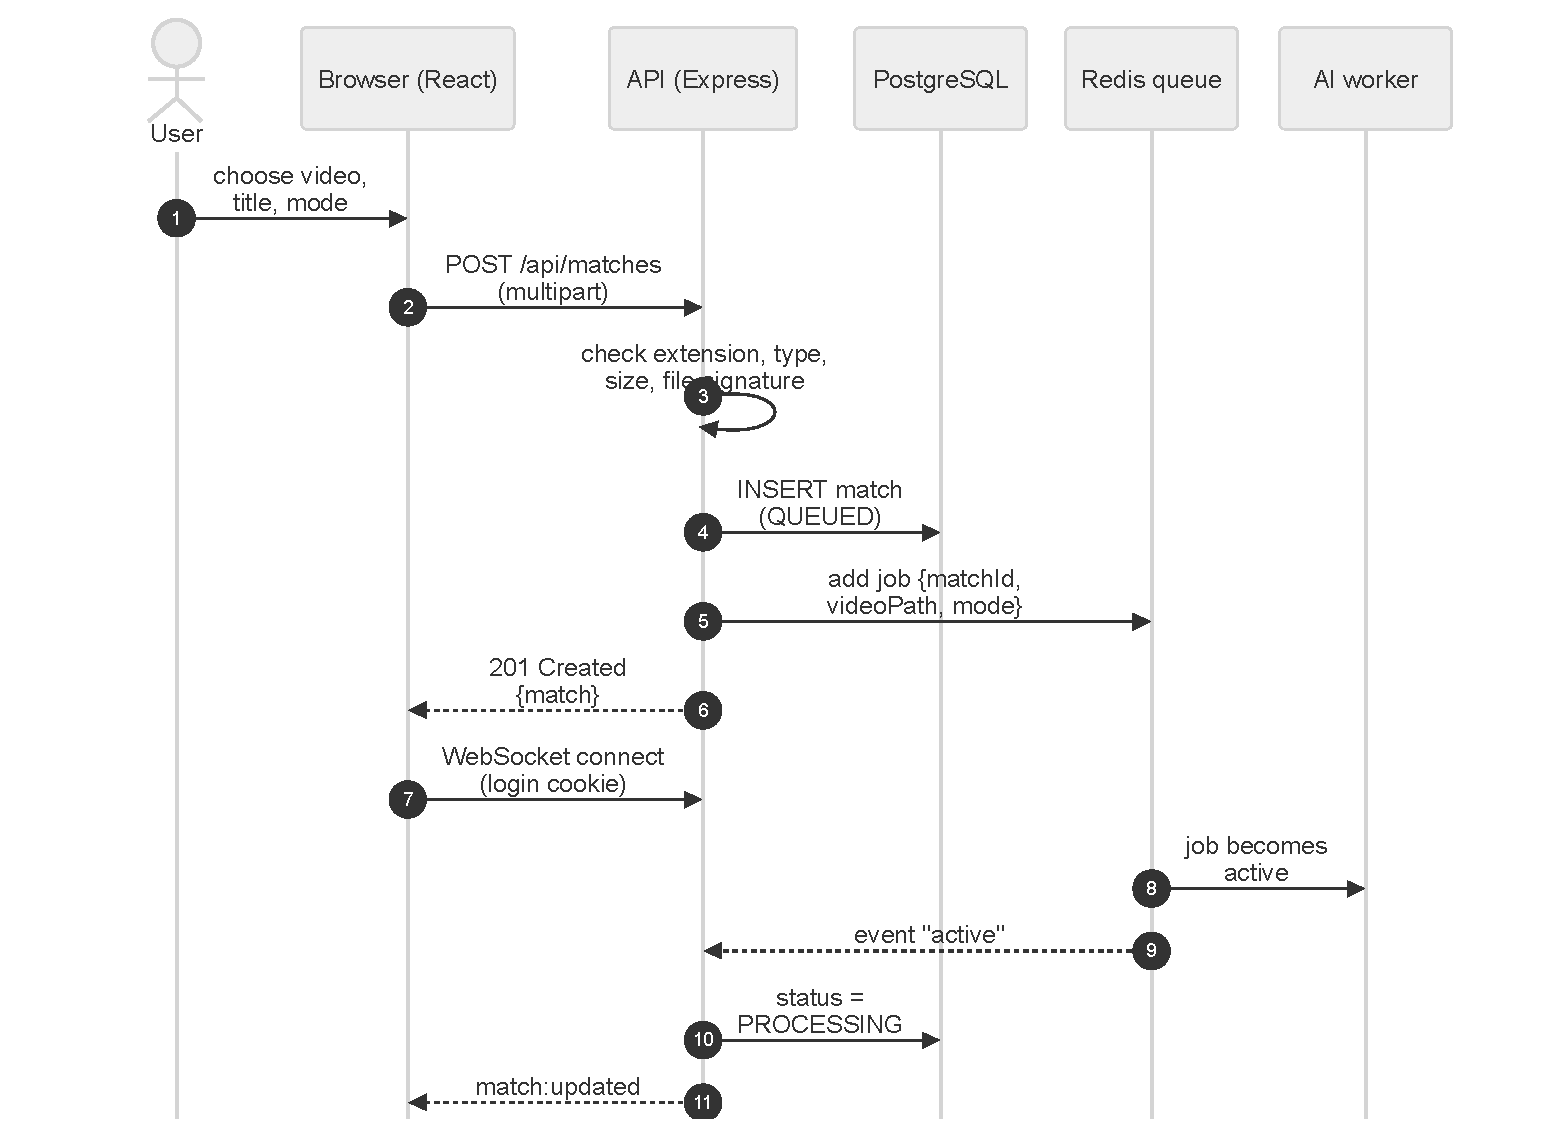
\includegraphics[width=\linewidth,height=0.86\textheight,keepaspectratio]{sequence_upload}
		\caption{Sequence of an upload, part 1: storing the video and queueing the job}
		\label{fig:sequence}
	\end{figure}
\end{landscape}

\begin{landscape}
	\begin{figure}
		\centering
		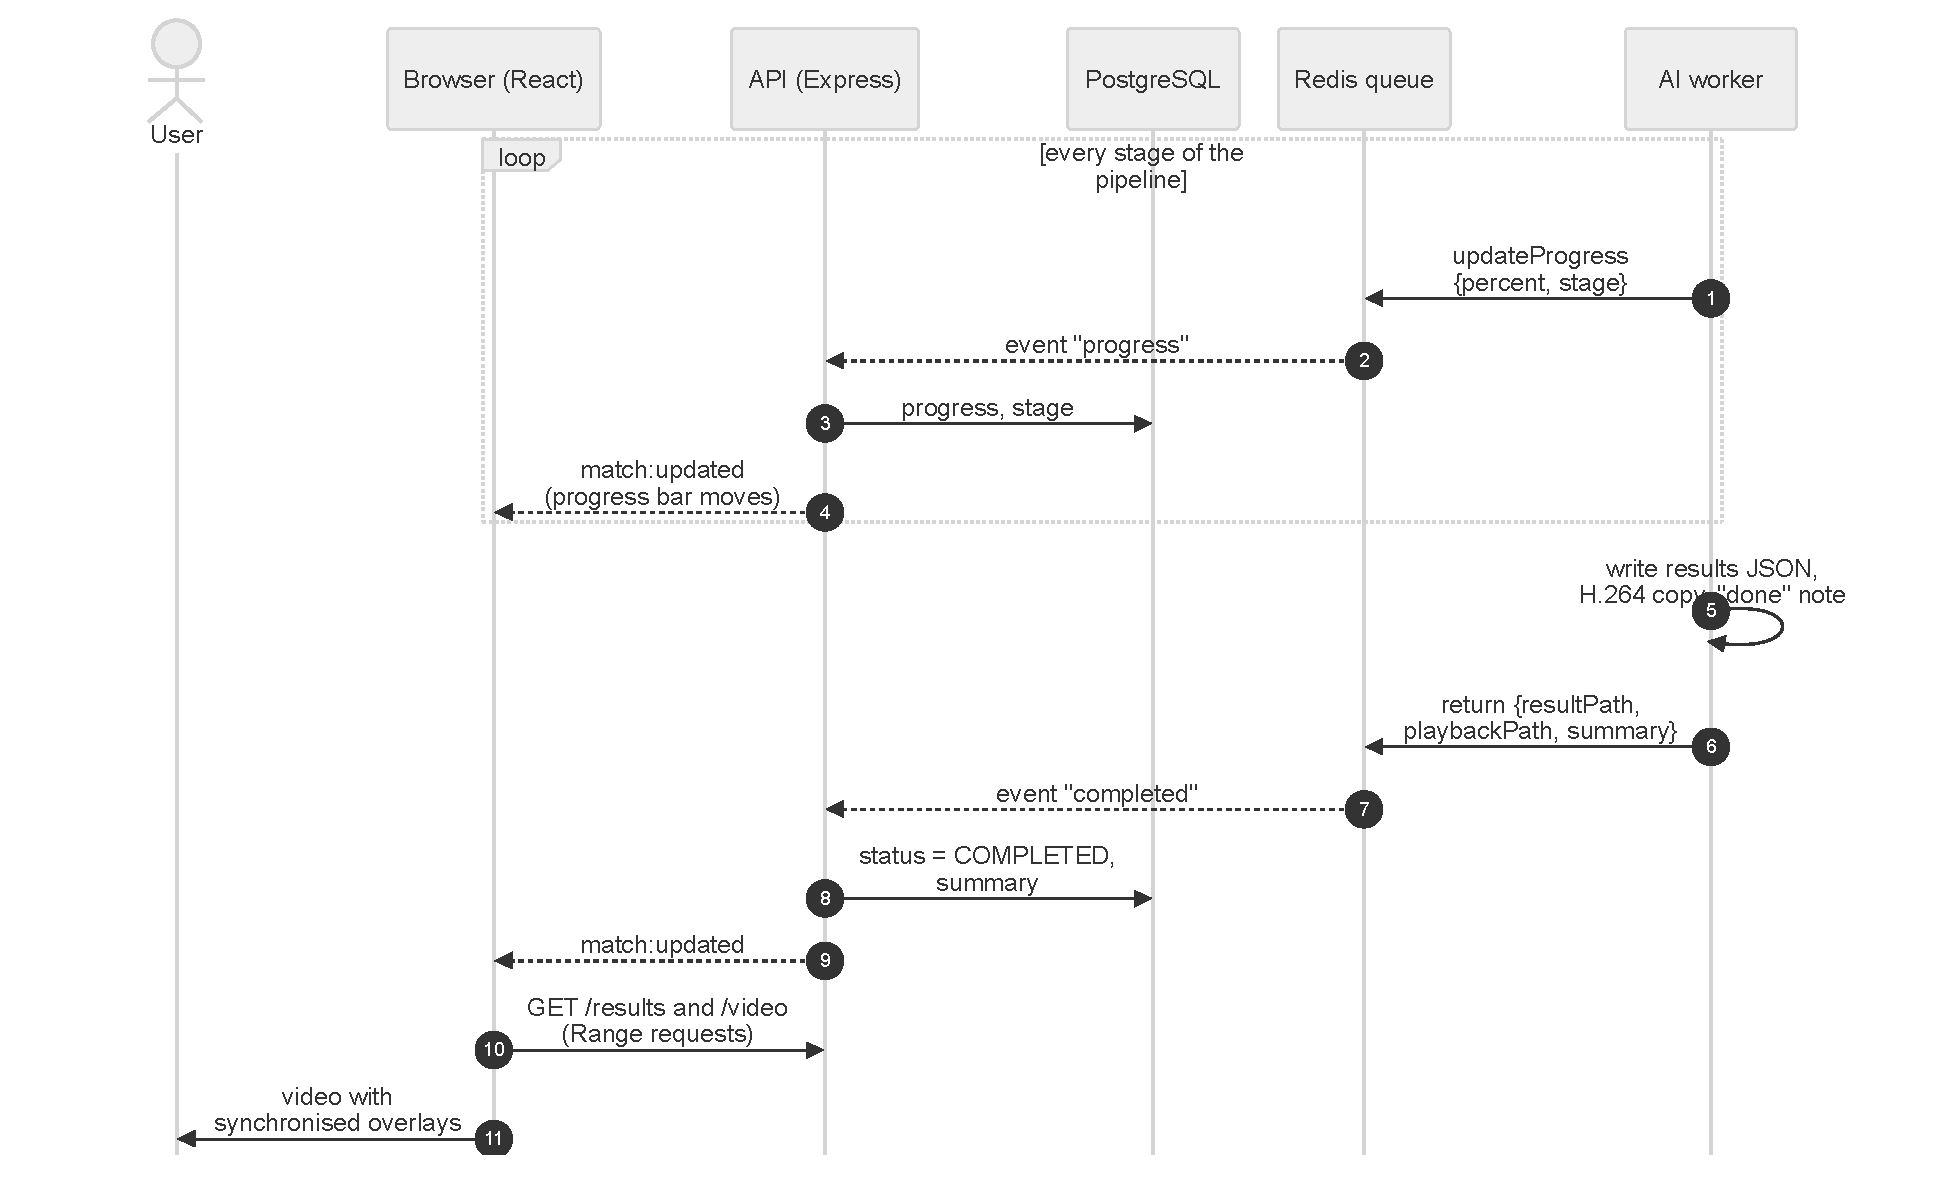
\includegraphics[width=\linewidth,height=0.86\textheight,keepaspectratio]{sequence_progress}
		\caption{Sequence of an upload, part 2: live progress, completion and playback}
		\label{fig:sequence-progress}
	\end{figure}
\end{landscape}

\section{Deployment and CI/CD}

\subsection{Containers}

Every service has its own \texttt{Dockerfile}, and \texttt{docker-compose.\allowbreak{}yml} describes how they work together (\autoref{fig:deployment}). The file uses a Compose profile: \texttt{docker compose up -d} starts only PostgreSQL and Redis, which suits development, when the three application services run directly on the developer's machine with hot reloading, while \texttt{docker compose --profile app up -d --build} starts the whole platform.

\begin{landscape}
	\begin{figure}
		\centering
		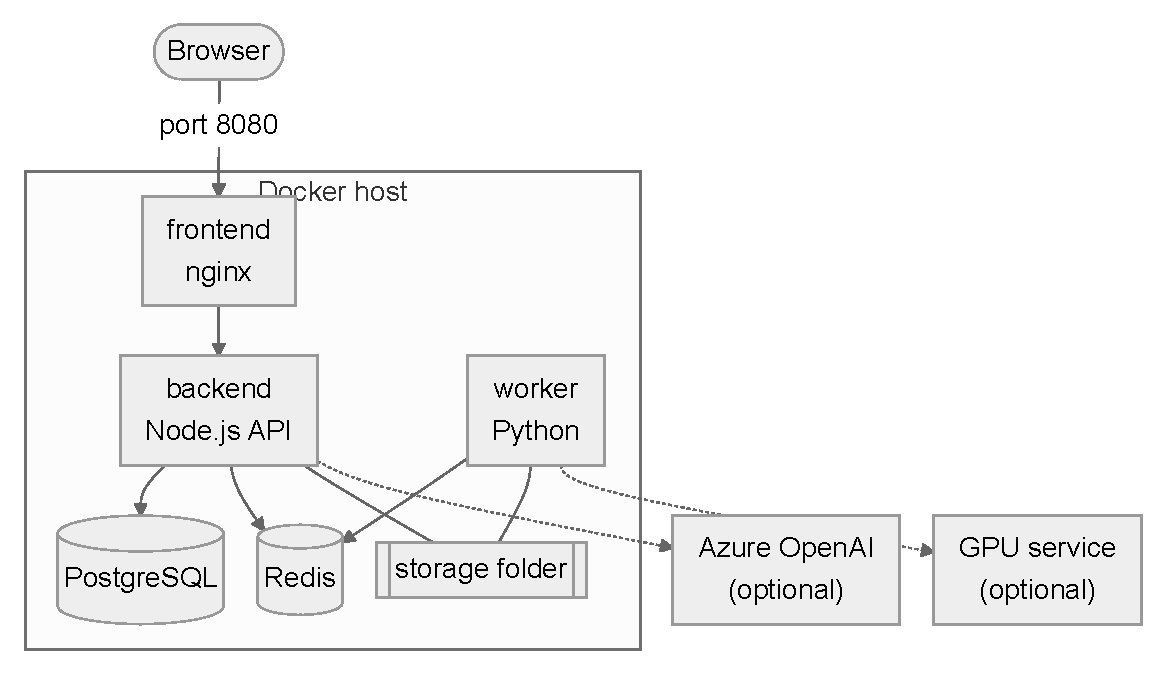
\includegraphics[width=\linewidth,height=0.86\textheight,keepaspectratio]{deployment}
		\caption{Deployment diagram}
		\label{fig:deployment}
	\end{figure}
\end{landscape}

\begin{table}[H]
	\centering
	\small
	\begin{tabular}{|p{0.11\textwidth}|p{0.22\textwidth}|p{0.58\textwidth}|}
		\hline
		\textbf{Service} & \textbf{Base image} & \textbf{Build and start-up} \\
		\hline
		frontend & \texttt{node:24-alpine} $\rightarrow$ \texttt{nginx:1.27-alpine} & Multi-stage build: the first stage runs \texttt{npm ci} and \texttt{npm run build}; only the static output is copied into the small nginx image. \\
		\hline
		backend & \texttt{node:24-alpine} & \texttt{npm ci} and \texttt{prisma generate}; on start, \texttt{prisma migrate deploy} applies pending migrations, then the API starts. Health check on \texttt{/api/health}. \\
		\hline
		worker & \texttt{python:3.12-slim} & OpenCV's system libraries, the CPU build of PyTorch and the pinned requirements. The models are mounted read-only from \texttt{worker/models}, so the image (about 3.4\,GB) contains no model files. \\
		\hline
		postgres & \texttt{postgres:17-alpine} & Data in a named volume; health check with \texttt{pg\_\allowbreak{}isready}. \\
		\hline
		redis & \texttt{redis:7.4-alpine} & Append-only file enabled, so queued jobs survive a Redis restart; health check with \texttt{redis-cli ping}. \\
		\hline
	\end{tabular}
	\caption{Container images}
	\label{tab:images}
\end{table}

The backend and worker containers mount the same \texttt{./storage} folder at \texttt{/storage}. The database stores only relative paths such as \texttt{videos/3f2a\dots.\allowbreak{}mp4}, and each service joins them with its own \texttt{STORAGE\_\allowbreak{}DIR}, so both agree on the files although they see the folder at different absolute paths.

\subsection{Reverse proxy}

In the container deployment the browser only talks to nginx on port 8080. nginx serves the built dashboard and forwards \texttt{/api/} and \texttt{/socket.\allowbreak{}io/} to the backend (\autoref{code:nginx}). Because everything comes from one origin, the log-in cookie and the WebSocket need no cross-origin configuration. Uploads are streamed straight through (\texttt{proxy\_\allowbreak{}request\_\allowbreak{}buffering off}), and the body limit matches the API's 1\,GB limit. Unknown paths such as \texttt{/matches/abc} return \texttt{index.\allowbreak{}html}, so deep links into the single-page application work.

\begin{lstlisting}[style=plain, caption={nginx configuration (excerpt from \texttt{frontend/nginx.\allowbreak{}conf})}, label={code:nginx}]
client_max_body_size 1050m;   # the API's 1 GB limit plus form overhead

location /api/ {
    proxy_pass http://backend:4000;
    proxy_request_buffering off;  # stream uploads straight to the API
    proxy_read_timeout 300s;
}
location /socket.io/ {
    proxy_pass http://backend:4000;
    proxy_http_version 1.1;
    proxy_set_header Upgrade $http_upgrade;  # WebSocket handshake
    proxy_set_header Connection "upgrade";
}
location / {
    try_files $uri $uri/ /index.html;       # single-page app fallback
}
\end{lstlisting}

\subsection{Continuous integration and delivery}
\label{sec:cicd}

The GitHub Actions workflow \texttt{.\allowbreak{}github/workflows/ci.\allowbreak{}yml} runs on every push and pull request (\autoref{fig:cicd}). Three jobs run in parallel. The backend job starts PostgreSQL and Redis as service containers, type-checks the API and runs its 42 Vitest and SuperTest tests against a real test database. The frontend job lints the code with oxlint, runs the 23 unit tests of the overlay mathematics and builds the production bundle, which includes the TypeScript check. The worker job installs the CPU build of PyTorch and runs the 43 pytest tests.

When all three pass, the system job downloads the two AI models (cached between runs), starts the whole platform with Docker Compose and runs the 11 system tests against it from the outside, including a real analysis of a 3-second clip and the cancelling of a running analysis. Only then does the images job build the three Docker images; on pushes to \texttt{main} it also publishes them to the GitHub Container Registry, tagged \texttt{latest} and with the commit hash. Every published image has therefore passed every test level, and any earlier version can be redeployed. \autoref{ch:testing} describes the tests themselves.

\begin{figure}[H]
	\centering
	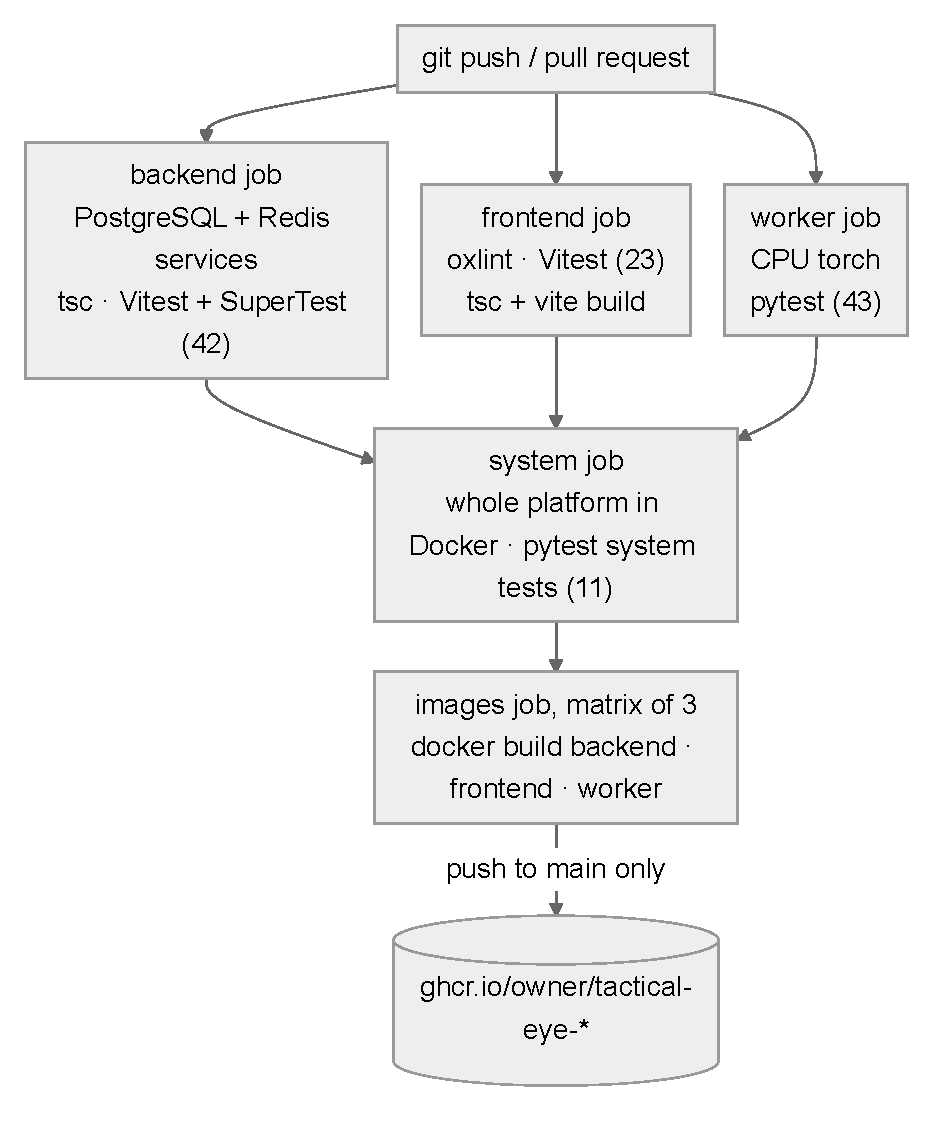
\includegraphics[width=0.7\textwidth]{cicd}
	\caption{The CI/CD pipeline}
	\label{fig:cicd}
\end{figure}

\subsection{Configuration}

All settings come from environment variables (\autoref{tab:env}). Locally they are read from the \texttt{.\allowbreak{}env} file in the repository root; in Docker, Compose passes them to the containers. The API checks its configuration with a Zod schema at start-up (\autoref{code:config}), so a missing or malformed value stops the server at once with a clear message instead of failing later inside a request. Secrets exist only in \texttt{.\allowbreak{}env}, which version control ignores.

\begin{lstlisting}[language=TypeScript, caption={Validated configuration (excerpt from \texttt{backend/src/config.\allowbreak{}ts})}, label={code:config}]
const EnvSchema = z.object({
  DATABASE_URL: z.string().min(1),
  REDIS_URL: z.string().default("redis://localhost:6379"),
  JWT_SECRET: z.string().min(32, "JWT_SECRET must be at least 32 characters"),
  // 1 GB: enough for a full half of a match (about 45 minutes).
  MAX_UPLOAD_MB: z.coerce.number().positive().default(1024),
  COOKIE_SECURE: z.enum(["true", "false"]).optional(),
});
const parsed = EnvSchema.safeParse(process.env);
if (!parsed.success) {
  console.error("Invalid configuration:\n" + z.prettifyError(parsed.error));
  process.exit(1);
}
\end{lstlisting}

\section{Data design}

The database contains two tables (\autoref{fig:er}) that are defined by the Prisma Schema. From this schema, Prisma creates a typed Client and an SQL migration for every modification. Each \texttt{User} will contain an ID, email address (unique and converted to all lower-case characters), name, bcrypt password hash and creation time. \autoref{tab:match-table} describes the \texttt{Match} table.

\begin{figure}[H]
	\centering
	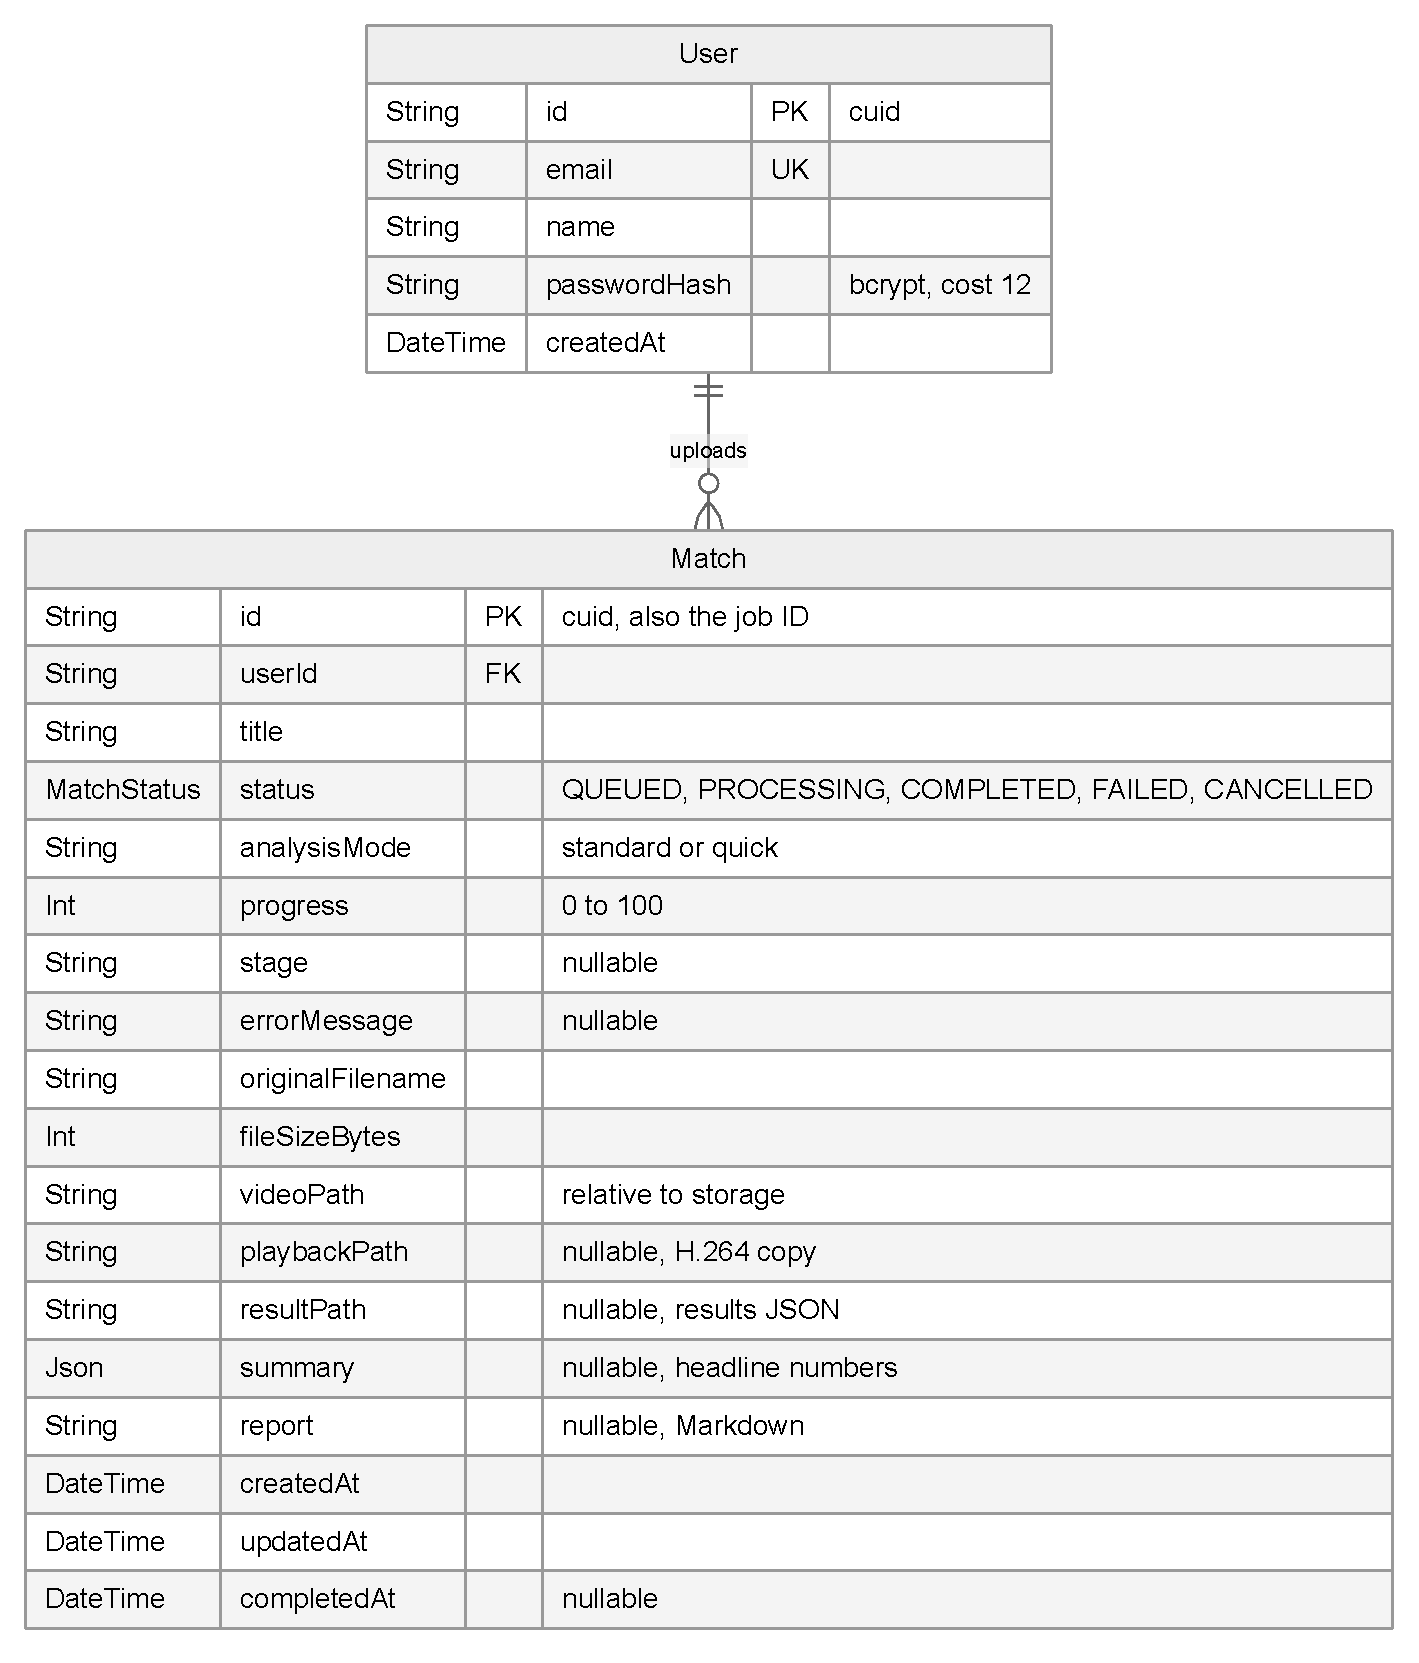
\includegraphics[width=\textwidth]{er}
	\caption{Entity-relationship diagram}
	\label{fig:er}
\end{figure}

\begin{table}[H]
	\centering
	\begin{tabular}{|p{0.24\textwidth}|p{0.67\textwidth}|}
		\hline
		\textbf{Column} & \textbf{Description} \\
		\hline
		id & Unique ID; also the ID of the queue job, so queue events map straight to rows. \\
		\hline
		userId & Owner; deleting a user deletes their matches. \\
		\hline
		title, analysisMode & Title, and \texttt{standard} or \texttt{quick}. \\
		\hline
		status, progress, stage & State (\autoref{fig:status}), 0--100 and the current step. \\
		\hline
		errorMessage & Reason of the last failure. \\
		\hline
		videoPath, playbackPath, resultPath & The upload, its browser-playable copy and the results file, relative to the storage folder. \\
		\hline
		summary & Headline numbers (JSON) for lists and the summary tab. \\
		\hline
		report & The AI coaching report (Markdown). \\
		\hline
		createdAt, completedAt & Creation and completion time. \\
		\hline
	\end{tabular}
	\caption{The \texttt{Match} table}
	\label{tab:match-table}
\end{table}

\begin{figure}[H]
	\centering
	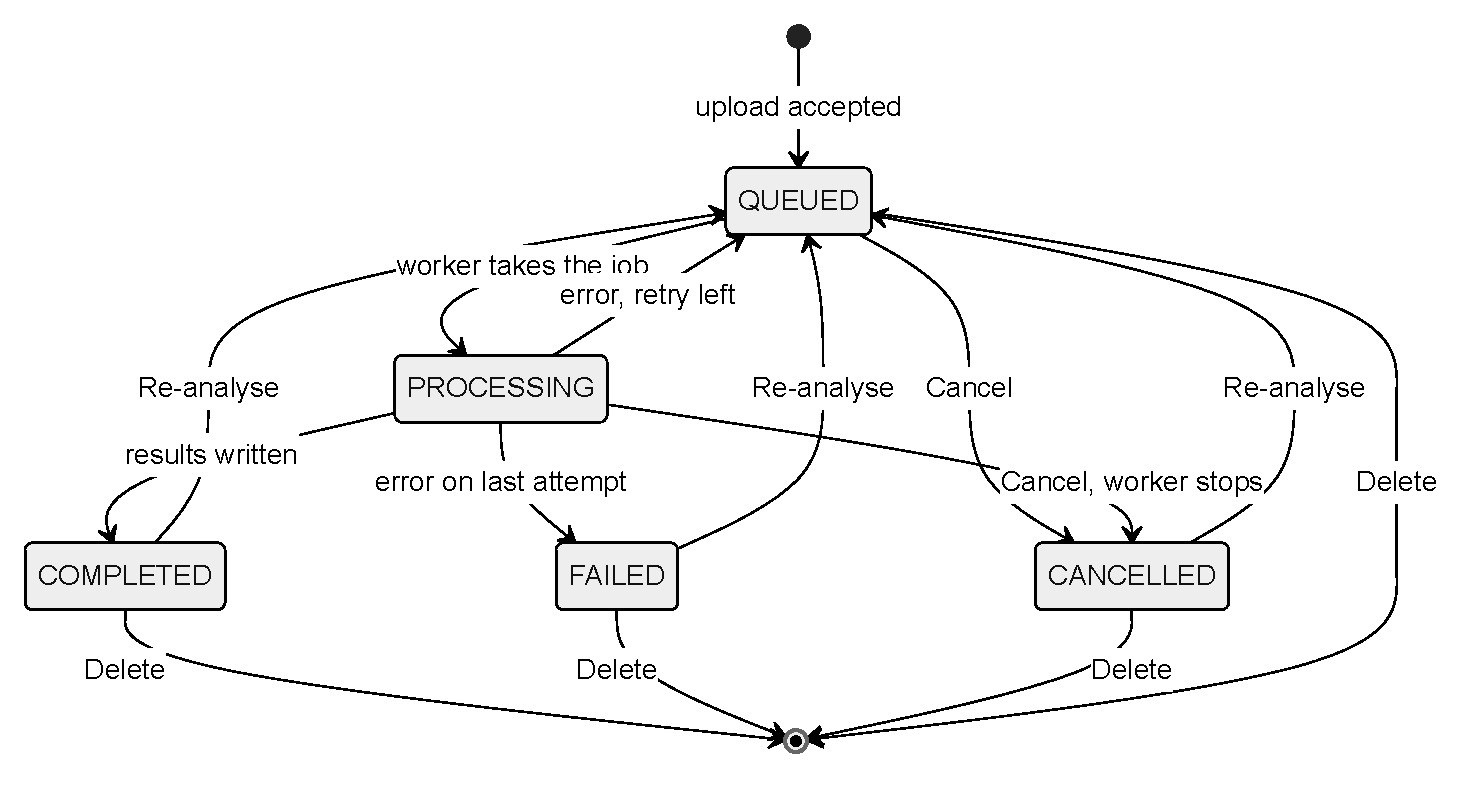
\includegraphics[width=\textwidth]{status}
	\caption{States of a match}
	\label{fig:status}
\end{figure}

The large analysis result files have been intentionally excluded from the database; it would be too much to store every single result in the database (each half generates a 54\,MB results file), but since the results file is stored on the hard drive, the API can serve it from there. Database holds only the small summary. The results file is the contract between the worker and the dashboard (\autoref{tab:results}). A person is represented as a compact array (as opposed to an object) resulting in a smaller file.

\begin{table}[H]
	\centering
	\begin{tabular}{|p{0.2\textwidth}|p{0.7\textwidth}|}
		\hline
		\textbf{Field} & \textbf{Content} \\
		\hline
		video & Frame rate, size, length, and which frames were analysed. \\
		\hline
		teams & Kit colour of each team and the goal it defends. \\
		\hline
		frames & For every analysed frame: each person (track ID, team, role, box, pitch position, position label), the ball, and the camera matrix of the frame. \\
		\hline
		players & For every position of a team: label (e.g. LB), time visible, distance, average and top speed, heatmap. \\
		\hline
		teamShape & Per frame and team: area, width and depth of the outfield players. \\
		\hline
		heatmaps & Where Team A, Team B and the ball spent their time. \\
		\hline
		formations & The formation, runner-up and cost of each team in every 5-second window, and the moments it changed. \\
		\hline
	\end{tabular}
	\caption{Main fields of the results file}
	\label{tab:results}
\end{table}

Files are stored within the common directory used by both the API and Worker: \texttt{videos/} stores all uploaded videos (with unique names) as well as the playback copies, while \texttt{results/} stores all result files. The API never accepts a file path from an external source; every stored path is resolved and refused if it leaves the storage folder, and the worker repeats the check before opening a file.

Each job placed into the \texttt{match-analysis} queue includes the match ID, video path, and mode. During execution, the worker sends updates on its status and current task at which point it will send the paths of results, playback copy and summary upon completion. If the worker fails to complete the task, it will return an error message which will be presented to the user. Each job has two chances at completing the task, waiting 10 seconds between each chance.

\section{The analysis pipeline}
\label{sec:pipeline}

The most difficult part of this project would be the analysis. \texttt{run\_\allowbreak{}analysis()} in \texttt{pipeline.py} chains the stages in \autoref{fig:pipeline}; each stage is a separate module being responsible for taking and returning a pandas table representing detections, one row per detection per frame. My initial build and tuning were done using 30-second clip files. When I ran it on both of my half-length videos, I found many issues which were masked by the clips, thus some of the things I have described below were to correct those problems.

\begin{figure}[H]
	\centering
	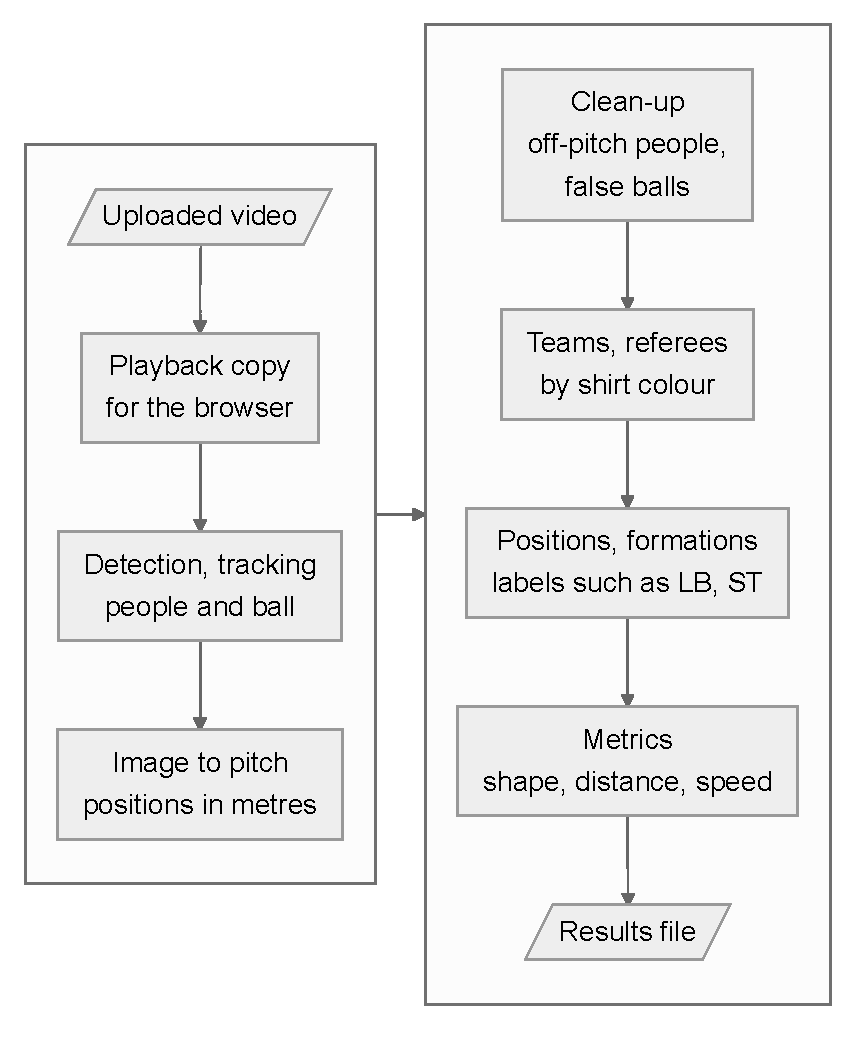
\includegraphics[width=0.65\textwidth]{pipeline}
	\caption{The stages of the analysis pipeline}
	\label{fig:pipeline}
\end{figure}

\subsection{Video input}

The worker first re-encodes the upload into an H.264 copy that every browser can play, with exactly one output frame per input frame so the overlays stay in sync. All later stages read this copy rather than the original: the two halves were encoded in AV1, and OpenCV failed with ``Corrupt frame detected'' whenever it had to jump within them. Frames are read in batches of four, so even a full half never sits in memory. Standard mode analyses every second frame of a 25\,fps video; for 50\,fps video the step is doubled, so every video is analysed at the same rate per second of play.

\subsection{Detection and tracking}

YOLOv8~\cite{yolov8}, with weights trained on broadcast football~\cite{roboflowsports}, finds players, goalkeepers, referees and the ball in each analysed frame. ByteTrack~\cite{bytetrack} links the people into tracks with stable IDs; it predicts each track's next position and matches new detections to it, including low-confidence detections of partly hidden players. The ball is not tracked this way, because it moves too fast; the five most likely ball candidates per frame are kept and the real one is chosen later.

\subsection{From the image to the pitch}

To measure in metres, each player's foot point is converted from image pixels to pitch coordinates. The pitch is a plane, and the mapping between a plane and its image is a homography~\cite{hartley}, a $3 \times 3$ matrix $H$:
\begin{equation}
	(X, Y, W)^T = H \, (x, y, 1)^T, \qquad \text{pitch point} = (X/W,\; Y/W).
\end{equation}
A second YOLOv8 model finds up to 32 known pitch landmarks in the image, such as the corners of the penalty areas (\autoref{fig:keypoints}). Their real positions on a $105 \times 68$\,m pitch are known, so $H$ can be fitted from them with RANSAC~\cite{ransac}, which ignores single wrongly detected landmarks. Because the camera pans and zooms, a new $H$ is fitted every few frames.

\begin{figure}[H]
	\centering
	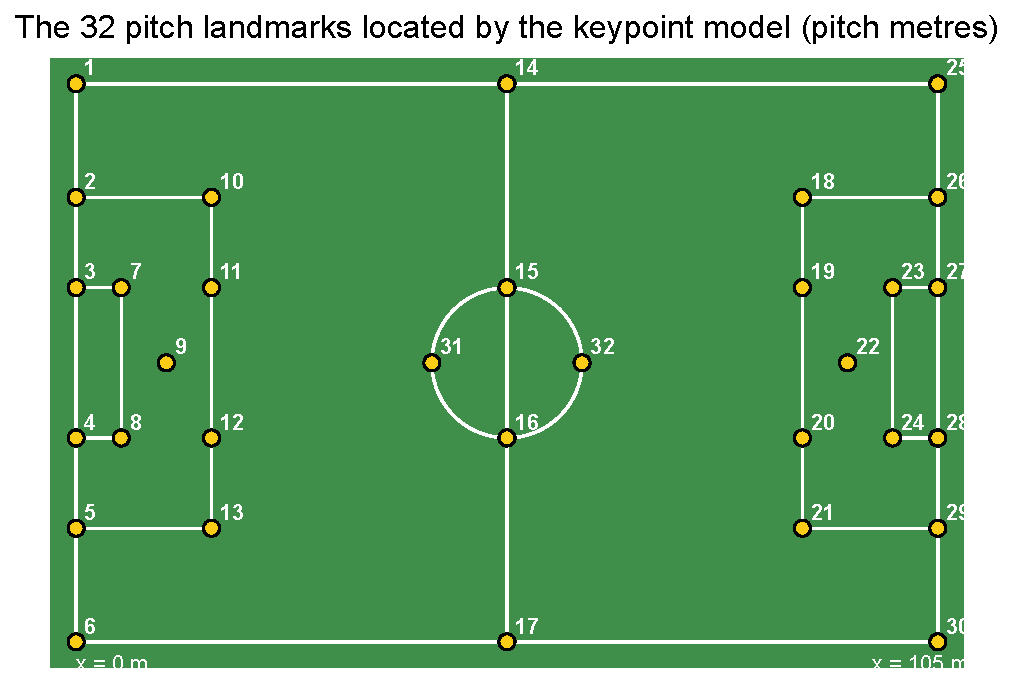
\includegraphics[width=0.85\textwidth]{pitch_keypoints}
	\caption{The 32 pitch landmarks}
	\label{fig:keypoints}
\end{figure}

Each fit is made on its own, so neighbouring fits can disagree slightly even though the real camera moved smoothly. On the first full half this made all movement paths jump across the video whenever a new fit arrived. The worker therefore smooths the camera model: it follows where four fixed points of the picture land on the pitch, smooths those positions over 1.5 seconds with a running median, and rebuilds $H$ from them. This cut the large jumps by about three quarters (\autoref{fig:camera-wobble}) while moving player positions by a median of only 0.16\,m.

\begin{figure}[H]
	\centering
	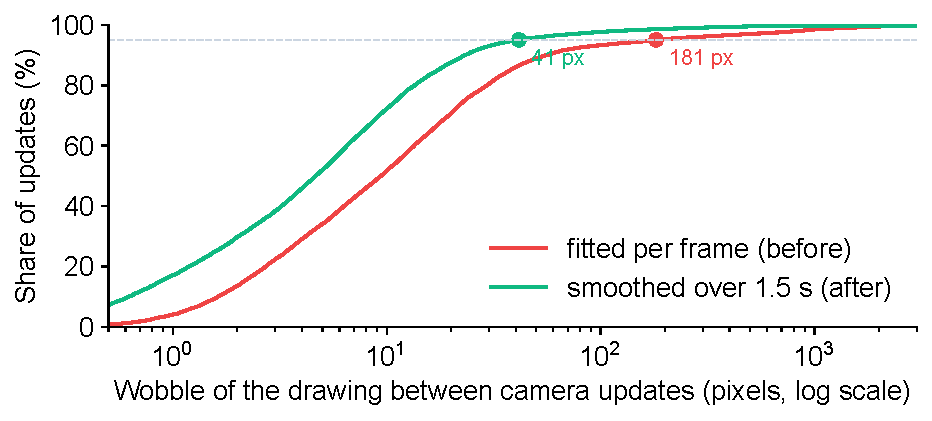
\includegraphics[width=0.9\textwidth]{camera_wobble}
	\caption{Jumps of the camera model before and after smoothing}
	\label{fig:camera-wobble}
\end{figure}

\subsection{Clean-up}
\label{sec:cleanup}

During stoppages a full half showed the touchline, where substitutes and staff stand, and spare balls lying beside it. With positions in metres both are easy to remove. A person whose usual (median) position is more than 0.5\,m outside the pitch lines is not part of the game and is removed; deciding over the whole track keeps a player who steps out for a throw-in. For the ball, the candidate closest to where the ball was a moment ago is kept, as long as the ball could have got there (no shot is faster than about 40\,m/s); candidates off the pitch and on the penalty spots are ignored when the path restarts. On the first half this removed 258 tracks of sideline people, and the share of ball positions off the pitch fell from 12\,\% to 0. \autoref{fig:ball-candidates} shows a stoppage after a goal, in which the old rule placed the ball on a spare ball beyond the far touchline in 344 of 375 frames.

\begin{figure}[H]
	\centering
	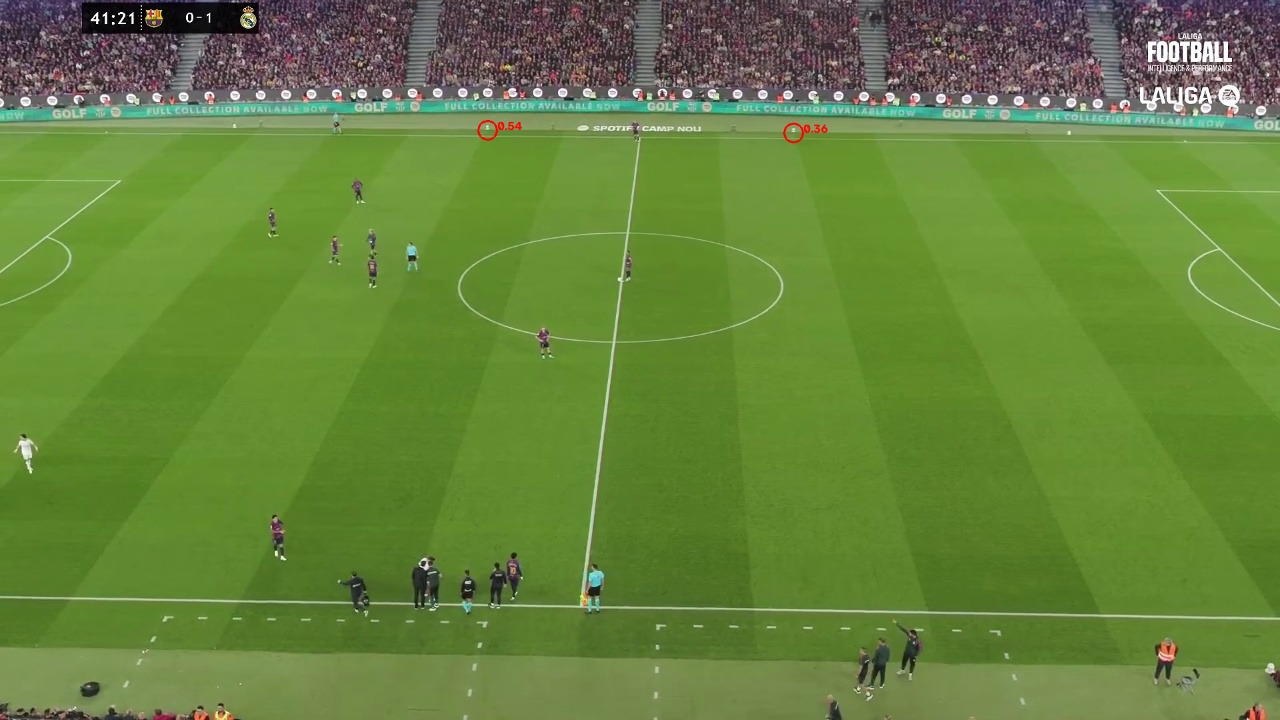
\includegraphics[width=\textwidth]{ball_candidates}
	\caption{Ball candidates during a stoppage: the two red circles are spare balls behind the far touchline, which the old rule took for the match ball}
	\label{fig:ball-candidates}
\end{figure}

\subsection{Teams and referees}

Players are split into teams by shirt colour. For each track, the torso region of up to ten detections is cropped, the grass colour measured around the player is removed, and the remaining pixels give the shirt colour in the CIE Lab colour space~\cite{opencvlab}. K-Means~\cite{kmeans} then splits the tracks into two teams. Goalkeepers wear a different kit, so they join the team whose players are closest to them.

The detector often called the main referee a player, and he then joined a team. The referee kit colour is therefore learned from the tracks the model does call referees (usually the assistants), and a ``player'' whose shirt is much closer to that colour than to either team colour becomes a referee. To choose ``much closer'', I ranked the candidate tracks and looked at a crop of each: below a ratio of about 0.65 almost all were officials, and from 0.68 white Real Madrid players appeared. A goalkeeper is only checked if he stands outside both penalty areas, because goalkeepers also wear a colour unlike both teams.

\subsection{Joining tracks and position labels}
\label{sec:positions}

ByteTrack starts a new track whenever it loses a player for two seconds, and the first half produced 1,423 tracks for about 25 people. Tracks that end and start again within five seconds, nearby and with the same team, are joined with the Hungarian algorithm~\cite{hungarian}, which left 555. Fewer is not possible with one camera: a player who is out of view for half a minute cannot be recognised, because all players of a team wear the same kit and shirt numbers are only a few pixels tall.

Instead of track numbers, players are therefore labelled by position. The formation step (below) assigns every visible player to a slot of the team's formation, such as LB or ST; these slots become the labels, smoothed over time so that they do not flicker. A label follows the position, not the person: if two players swap sides, their labels swap too.

\subsection{Formations}

A formation cannot be seen in a single frame, so the average positions of a team's outfield players are computed over 5-second windows, scaled to a unit square and compared with nine formation templates (\autoref{fig:templates}). The cost of a template is the mean distance between players and slots under the best one-to-one assignment, found with the Hungarian algorithm (\autoref{fig:matching}). A new formation is only accepted when it fits clearly better than the current one and has lasted 20 seconds; without this rule the first half reported 282 formation changes instead of 14.

\begin{figure}[H]
	\centering
	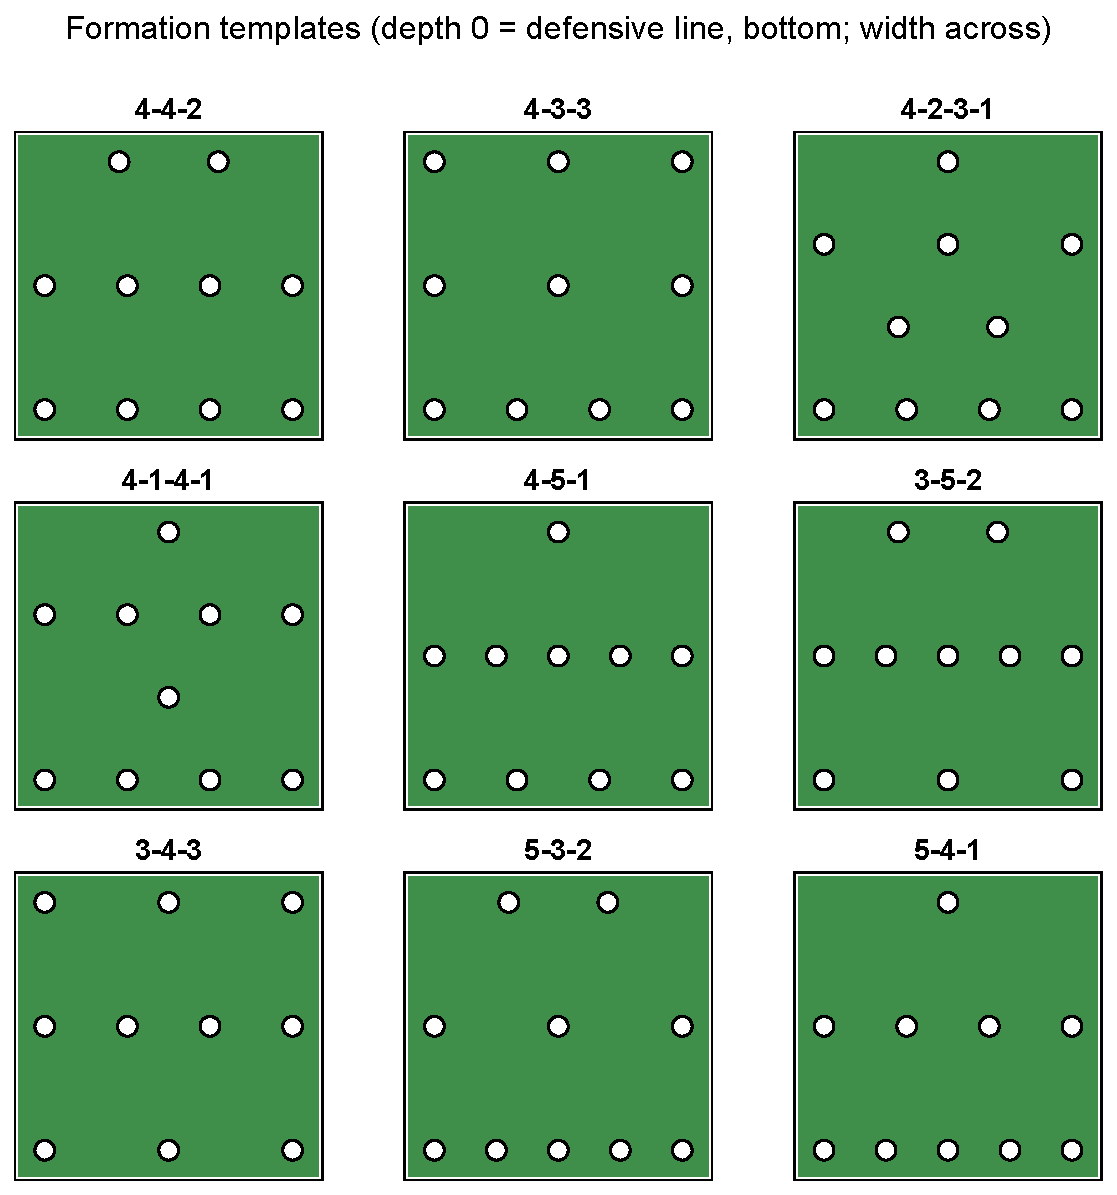
\includegraphics[width=0.62\textwidth]{formation_templates}
	\caption{The nine formation templates}
	\label{fig:templates}
\end{figure}

\begin{figure}[H]
	\centering
	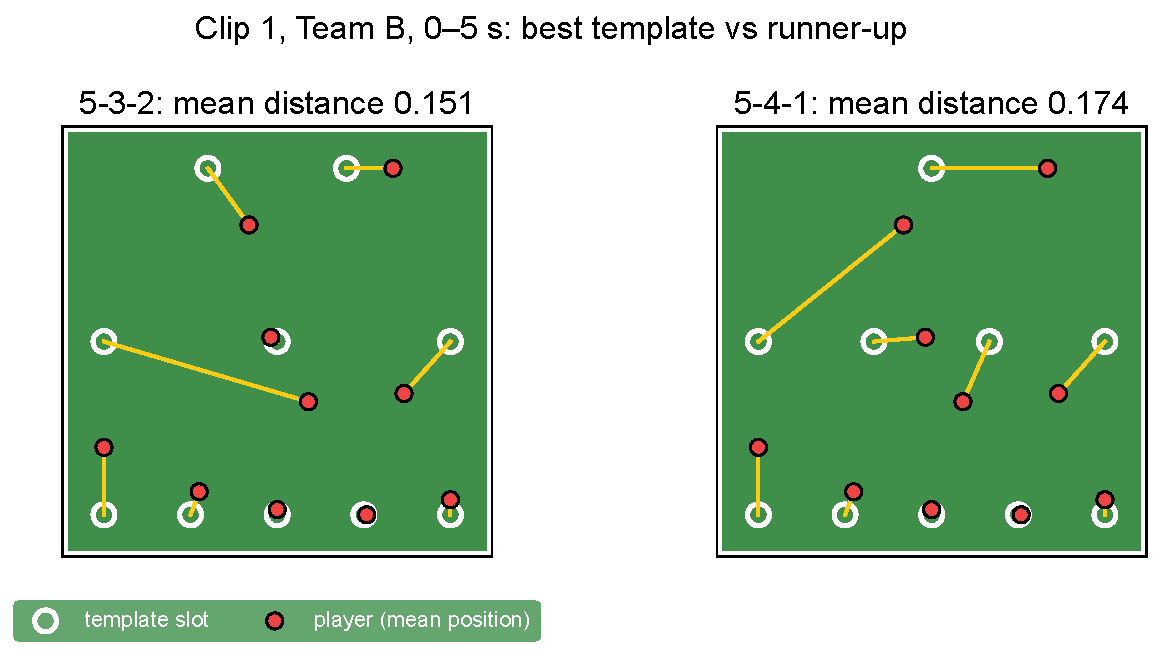
\includegraphics[width=\textwidth]{formation_matching}
	\caption{Matching one window of a team to the best template and the runner-up}
	\label{fig:matching}
\end{figure}

\subsection{Metrics}
\label{sec:metrics}

The worker determines each team’s compactness (the area of the convex hull of its outfield players), width and depth per frame from the smoothed positions, and the distance travelled by each position, how long it was in view, the average speed, and a heatmap for every position. Any steps with speeds greater than 12\,m/s will be considered as tracking errors and are ignored. The top speed is the best average over one second versus the fastest single step; an earlier version incorrectly reported 39.6\,km/h on one clip due to a single displaced position being considered a sprint.

\section{The backend (API)}

\subsection{Module structure}

The API in \texttt{backend/src/} is an Express 5 application in TypeScript, executed with \texttt{tsx}. \autoref{tab:api-modules} lists its modules.

\begin{longtable}{|p{0.20\textwidth}|p{0.72\textwidth}|}
	\hline
	\textbf{Module} & \textbf{Responsibility} \\
	\hline
	\endhead
	\texttt{index.\allowbreak{}ts} & Entry point: creates the HTTP and Socket.IO servers on one port, authenticates WebSocket connections, starts the queue event listener, shuts down cleanly on SIGINT/SIGTERM. \\
	\hline
	\texttt{app.\allowbreak{}ts} & Builds the Express application: CORS, JSON body parser (1\,MB), cookie parser, routers, health endpoint, 404 handler and the central error handler. \\
	\hline
	\texttt{config.\allowbreak{}ts} & Loads \texttt{.\allowbreak{}env}, validates all settings with Zod, exposes a typed \texttt{config} object. \\
	\hline
	\texttt{db.\allowbreak{}ts} & The single shared Prisma client. \\
	\hline
	\texttt{auth.\allowbreak{}ts} & Signing and checking session tokens, cookie options, the \texttt{requireAuth} middleware. \\
	\hline
	\texttt{routes/auth.\allowbreak{}ts} & \texttt{/api/auth/*}: register, log in, log out, current user. \\
	\hline
	\texttt{routes/matches.\allowbreak{}ts} & \texttt{/api/matches/*}: upload, list, get, video streaming, results, re-analyse, cancel, report, delete. \\
	\hline
	\texttt{queue.\allowbreak{}ts} & The BullMQ queue: adding, removing and cancelling jobs, counting workers, and turning queue events into database updates. \\
	\hline
	\texttt{storage.\allowbreak{}ts} & Storage folders, safe resolution of stored paths, file deletion, video signature check. \\
	\hline
	\texttt{report.\allowbreak{}ts} & Builds the statistics for the language model, calls Azure OpenAI and translates its errors. \\
	\hline
	\texttt{colours.\allowbreak{}ts} & Turns a measured kit colour into a plain name for the report. \\
	\hline
	\texttt{matchView.\allowbreak{}ts} & \texttt{toPublicMatch()}: the form of a match sent to browsers, without internal file paths. \\
	\hline
	\caption{Modules of the API}
	\label{tab:api-modules}
\end{longtable}

\subsection{REST API}

All endpoints are under \texttt{/api} and exchange JSON, except uploads and file downloads. Errors always have the form \texttt{\{"error": "message"\}} with a fitting HTTP status. All match endpoints need a valid session cookie.

\begin{longtable}{|p{0.10\textwidth}|p{0.27\textwidth}|p{0.54\textwidth}|}
	\hline
	\textbf{Method} & \textbf{Path} & \textbf{Description and responses} \\
	\hline
	\endhead
	POST & \texttt{/auth/register} & Body \texttt{\{name, email, password\}}. Creates the user and sets the session cookie. 201; 400 invalid input; 409 e-mail exists. \\
	\hline
	POST & \texttt{/auth/login} & Body \texttt{\{email, password\}}. Sets the session cookie. 200 \texttt{\{user\}}; 401 wrong credentials. \\
	\hline
	POST & \texttt{/auth/logout} & Clears the cookie. 204. \\
	\hline
	GET & \texttt{/auth/me} & The logged-in user. 200 \texttt{\{user\}}; 401 not logged in or account deleted. \\
	\hline
	POST & \texttt{/matches} & Multipart form with \texttt{video}, \texttt{title}, \texttt{mode}. Stores the file, creates the match, queues the job. 201 \texttt{\{match\}}; 400 no or invalid file; 413 too large. \\
	\hline
	GET & \texttt{/matches} & The user's matches, newest first. 200 \texttt{\{matches\}}. \\
	\hline
	GET & \texttt{/matches/:id} & One match. 200 \texttt{\{match\}}; 404 not found or not owned. \\
	\hline
	GET & \texttt{/\allowbreak{}matches/\allowbreak{}:id/\allowbreak{}video} & Streams the playback copy (or the original) with HTTP Range support for seeking. 200 or 206. \\
	\hline
	GET & \texttt{/\allowbreak{}matches/\allowbreak{}:id/\allowbreak{}results} & The results file. 200; 409 not finished. \\
	\hline
	POST & \texttt{/\allowbreak{}matches/\allowbreak{}:id/\allowbreak{}reanalyse} & Optional body \texttt{\{mode\}}. Queues the analysis again. 200 \texttt{\{match\}}; 409 already queued or running. \\
	\hline
	POST & \texttt{/\allowbreak{}matches/\allowbreak{}:id/\allowbreak{}cancel} & Stops a queued or running analysis. 200 \texttt{\{match\}} (cancelled, or still processing with stage ``Cancelling\dots''); 409 not being analysed. \\
	\hline
	GET & \texttt{/\allowbreak{}matches/\allowbreak{}:id/\allowbreak{}report} & 200 \texttt{\{report, enabled\}}; \texttt{enabled} says whether reports are configured. \\
	\hline
	POST & \texttt{/\allowbreak{}matches/\allowbreak{}:id/\allowbreak{}report} & Generates and stores the report. 200 \texttt{\{report\}}; 409 not finished; 429, 502 or 503 report service errors. \\
	\hline
	DELETE & \texttt{/matches/:id} & Deletes the match, its waiting job and its files. 204; 409 while processing. \\
	\hline
	GET & \texttt{/health} & Database, Redis, number of workers and job counts. 200 when healthy, 503 otherwise. \\
	\hline
	\caption{REST endpoints}
	\label{tab:endpoints}
\end{longtable}

The WebSocket interface has one event. After connecting, the server puts each socket into a private room \texttt{user:<id>}; whenever one of the user's matches changes, it emits \texttt{match:updated} with the public match to that room only.

\subsection{Important functions}

\begin{longtable}{|p{0.22\textwidth}|p{0.26\textwidth}|p{0.43\textwidth}|}
	\hline
	\textbf{Function} & \textbf{Input $\rightarrow$ output} & \textbf{Activity} \\
	\hline
	\endhead
	\texttt{requireAuth} (auth.ts) & request $\rightarrow$ \texttt{req.\allowbreak{}userId}, or 401 & Reads the \texttt{token} cookie, checks the JWT signature and expiry, attaches the user ID. \\
	\hline
	\texttt{signToken} / \texttt{verifyToken} & user ID $\leftrightarrow$ JWT & HS256-signed token with the user ID as subject, valid for 7 days~\cite{jwt}. \\
	\hline
	\texttt{findOwnMatch} (matches.ts) & request $\rightarrow$ match, or 404 & Loads a match by ID \emph{and} owner; answers 404, not 403, for other users' matches so their IDs cannot be probed. \\
	\hline
	\texttt{isVideoFile} (storage.ts) & file path $\rightarrow$ boolean & Checks the first 12 bytes for the signatures of MP4/MOV, Matroska/WebM and AVI. \\
	\hline
	\texttt{absolutePath} (storage.ts) & relative path $\rightarrow$ absolute path & Refuses any path that would leave the storage folder. \\
	\hline
	\texttt{enqueueAnalysis} (queue.ts) & \texttt{\{matchId, videoPath, mode\}} $\rightarrow$ void & Removes a finished job with the same ID (BullMQ ignores duplicate IDs), deletes any old cancel note, adds the job with the match ID as job ID. \\
	\hline
	\texttt{requestCancel} (queue.ts) & match ID $\rightarrow$ \texttt{"removed"} or \texttt{"stopping"} & Removes a waiting job; if the job is running, writes the cancel note (expires after a day). A missing job counts as removed. \\
	\hline
	\texttt{cancelledState} (queue.ts) & match $\rightarrow$ database fields & \texttt{COMPLETED} with stage ``Re-analysis cancelled'' if the match has earlier results, otherwise \texttt{CANCELLED}. \\
	\hline
	\texttt{countWorkers} (queue.ts) & $\rightarrow$ number & Counts distinct worker connections in Redis's client list, recognising the Node.js and Python naming schemes. \\
	\hline
	\texttt{start\allowbreak{}Queue\allowbreak{}Event\allowbreak{}Listener} & callback $\rightarrow$ listener & Turns \texttt{active}, \texttt{progress}, \texttt{completed} and \texttt{failed} events into database updates and calls the callback with each updated match. \\
	\hline
	\texttt{buildMatchData} (report.ts) & match $\rightarrow$ statistics object & Reads the results file and builds the model's input: summary, kit colour names, formation timeline, shape per third of the video, the three positions that ran furthest. \\
	\hline
	\texttt{colourName} (colours.ts) & hex colour $\rightarrow$ name & HSL rules: white, black, greys, then a hue name with ``dark'' or ``light'' (\autoref{sec:report}). \\
	\hline
	\texttt{generate\allowbreak{}Coaching\allowbreak{}Report} & match $\rightarrow$ Markdown & Builds the statistics, calls the model, maps its errors to \texttt{ReportError} with an HTTP status. \\
	\hline
	\caption{Important functions of the API}
	\label{tab:api-functions}
\end{longtable}

\subsection{Upload handling}

Multer streams an upload to disk while it arrives, so even a 1\,GB video never has to fit in memory. The file gets a random UUID name, and only files with a video extension and a \texttt{video/*} MIME type are accepted. Both are supplied by the client and can be faked, so the API also reads the file's first bytes after the upload and deletes it if they are not those of a video container. Then the match row is created and the job queued. If the queue cannot be reached, the match is kept but marked failed with ``Could not queue the analysis job'', so the user can retry with Re-analyse instead of uploading again.

\subsection{Turning queue events into live updates}

The queue events of one job arrive in bursts, for example several progress events within milliseconds. In the first version each event started its own database update, a slower update sometimes finished after a newer one, and the progress bar jumped backwards. The listener now chains the updates of each match: every update waits for the previous update of the same match, while different matches proceed in parallel (\autoref{code:chain}). The \texttt{failed} event checks whether the job has attempts left; if so, the match goes back to \texttt{QUEUED} with ``Retrying after an error''. The \texttt{completed} event checks for \texttt{\{cancelled: true\}} and then applies \texttt{cancelledState} instead of storing results.

\begin{lstlisting}[language=TypeScript, caption={Per-match ordering of database updates (from \texttt{backend/src/queue.\allowbreak{}ts})}, label={code:chain}]
const chains = new Map<string, Promise<void>>();
const update = (matchId: string, data: MatchUpdate) => {
  const next = (chains.get(matchId) ?? Promise.resolve()).then(async () => {
    // Updates for matches deleted in the meantime are simply dropped.
    const match = await prisma.match.update({ where: { id: matchId }, data }).catch(() => null);
    if (match) onUpdate(match);   // push to the user's browser
  });
  chains.set(matchId, next);
  void next.finally(() => { if (chains.get(matchId) === next) chains.delete(matchId); });
  return next;
};
\end{lstlisting}

\subsection{Cancelling an analysis}
\label{sec:cancel}

The coach who uploads the wrong video, or picks Standard instead of Quick, should not have to wait an hour. A queued job is easy: BullMQ can remove a waiting job. A running job cannot be taken away from the worker that holds its lock, so the API leaves a note in Redis (\texttt{tactical-eye:cancel:<match\allowbreak{}Id>}) and shows ``Cancelling\dots''. The worker checks for the note every two seconds in a background task. When it finds one, it sets a flag, and the next progress report from the analysis thread raises \texttt{Analysis\allowbreak{}Cancelled}, which stops the pipeline wherever it is. The pipeline reports progress hundreds of times per analysis, so this needs no checks in the individual stages. The worker then deletes a half-written playback copy if the match had no earlier results and returns \texttt{\{cancelled: true\}}. When the analysis runs on the GPU, the worker also calls the GPU service's cancel endpoint, so the GPU becomes free for the next job. In the system test the worker stopped 4 seconds after the request.

\subsection{Error handling}

Express 5 forwards errors thrown in asynchronous handlers to the error middleware, so route code can simply throw. The central handler in \texttt{app.\allowbreak{}ts} turns validation errors (Zod) into 400 with a readable description of the invalid fields, upload errors (Multer) into 413 for oversized files and 400 otherwise, and everything else into 500 ``Internal server error'', logging the details on the server without showing them to the client. Expected errors (not found, wrong state) are answered in the routes with 404 or 409.

\subsection{The coaching report}
\label{sec:report}

\texttt{report.\allowbreak{}ts} prepares a compact summary of the match for the model: the stored summary, each team's kit colour, defended goal and formation timeline, the team shape averaged over each third of the video, the three positions that ran furthest, and the formation changes. It is sent with a system prompt that defines the sections and the rules: every statement must rest on the numbers, passes, shots and goals must never be invented, and the conclusions are tentative because the camera does not show every player.

The first reports said ``Team A (kit \#C7C9AA)'' and ``Player \#17'', which no coach can use. Two changes fixed this. \texttt{colourName} turns the measured colour into a plain name with simple HSL rules: very light colours with little saturation are white, colours with almost no chroma are black or a shade of grey, and the rest are named by hue with ``dark'' or ``light'' added by lightness. The rules allow for the camera making kits paler or greyer than they are, and dark blues count as colour much sooner than other hues, because navy kits look grey on video. A test checks the colours measured on the real videos: Real Madrid's \texttt{\#C7C9AA} is ``white'', PSG's \texttt{\#4E525D} ``navy'' and Barcelona's away kit \texttt{\#A27051} ``orange''. The runners are now sent as positions with full names (``LB (left back)''), and the prompt forbids colour codes and player numbers. A test also checks that the data sent to the model contains neither.

The request goes to a \texttt{gpt-5-mini} deployment on Azure OpenAI through the \texttt{AzureOpenAI} client of the official \texttt{openai} SDK, with a 120-second timeout and two automatic retries. The output limit is 8,000 tokens because reasoning models spend tokens on hidden reasoning before writing. I chose Azure OpenAI because its use is covered by the Azure for Students credit, and kept all provider-specific code in this one module.

\section{The AI worker}

\subsection{Modules}

\begin{longtable}{|p{0.22\textwidth}|p{0.70\textwidth}|}
	\hline
	\textbf{Module} & \textbf{Responsibility} \\
	\hline
	\endhead
	\texttt{worker.\allowbreak{}py} & Queue consumer: takes jobs, runs the analysis in a thread, forwards progress, watches for cancel notes, chooses between remote and local analysis, keeps the ``done'' notes. \\
	\hline
	\texttt{src/config.\allowbreak{}py} & Every parameter and threshold in one place, each with a comment explaining its value. \\
	\hline
	\texttt{src/pipeline.\allowbreak{}py} & \texttt{run\_\allowbreak{}analysis()}: runs the stages, reports progress, times each stage, measures memory, builds and writes the results and the summary. \\
	\hline
	\texttt{src/video.\allowbreak{}py}, \texttt{src/transcode.\allowbreak{}py} & Video metadata and batched frame reading; the H.264 playback copy. \\
	\hline
	\texttt{src/detector.\allowbreak{}py} & \texttt{Football\allowbreak{}Detector}: YOLOv8 inference and class mapping. \\
	\hline
	\texttt{src/tracker.\allowbreak{}py} & \texttt{FootballTracker}, \texttt{iter\_\allowbreak{}tracks}: ByteTrack and the tracks table. \\
	\hline
	\texttt{src/homography.\allowbreak{}py} & Pitch landmarks, homography fitting, smoothing and projection. \\
	\hline
	\texttt{src/cleanup.\allowbreak{}py} & Removing people off the pitch, choosing the real ball, joining broken tracks. \\
	\hline
	\texttt{src/clustering.\allowbreak{}py} & Roles, shirt colours, teams, referees, formation templates and detection. \\
	\hline
	\texttt{src/positions.\allowbreak{}py} & Slot names and the position labels. \\
	\hline
	\texttt{src/trajectories.\allowbreak{}py}, \texttt{src/metrics.\allowbreak{}py} & Smoothing and ball interpolation; team shape, statistics, heatmaps. \\
	\hline
	\texttt{src/cancel.\allowbreak{}py} & \texttt{Analysis\allowbreak{}Cancelled} and the name of the cancel note. \\
	\hline
	\texttt{src/remote.\allowbreak{}py}, \texttt{gpu\_\allowbreak{}server.\allowbreak{}py} & Client of the remote GPU service, and the service itself (FastAPI). \\
	\hline
	\caption{Modules of the worker}
	\label{tab:worker-modules}
\end{longtable}

The stage modules do not know about the queue or the web platform. They take and return DataFrames and can be used from scripts and tests. \autoref{fig:classes} shows the main classes.

\begin{figure}[H]
	\centering
	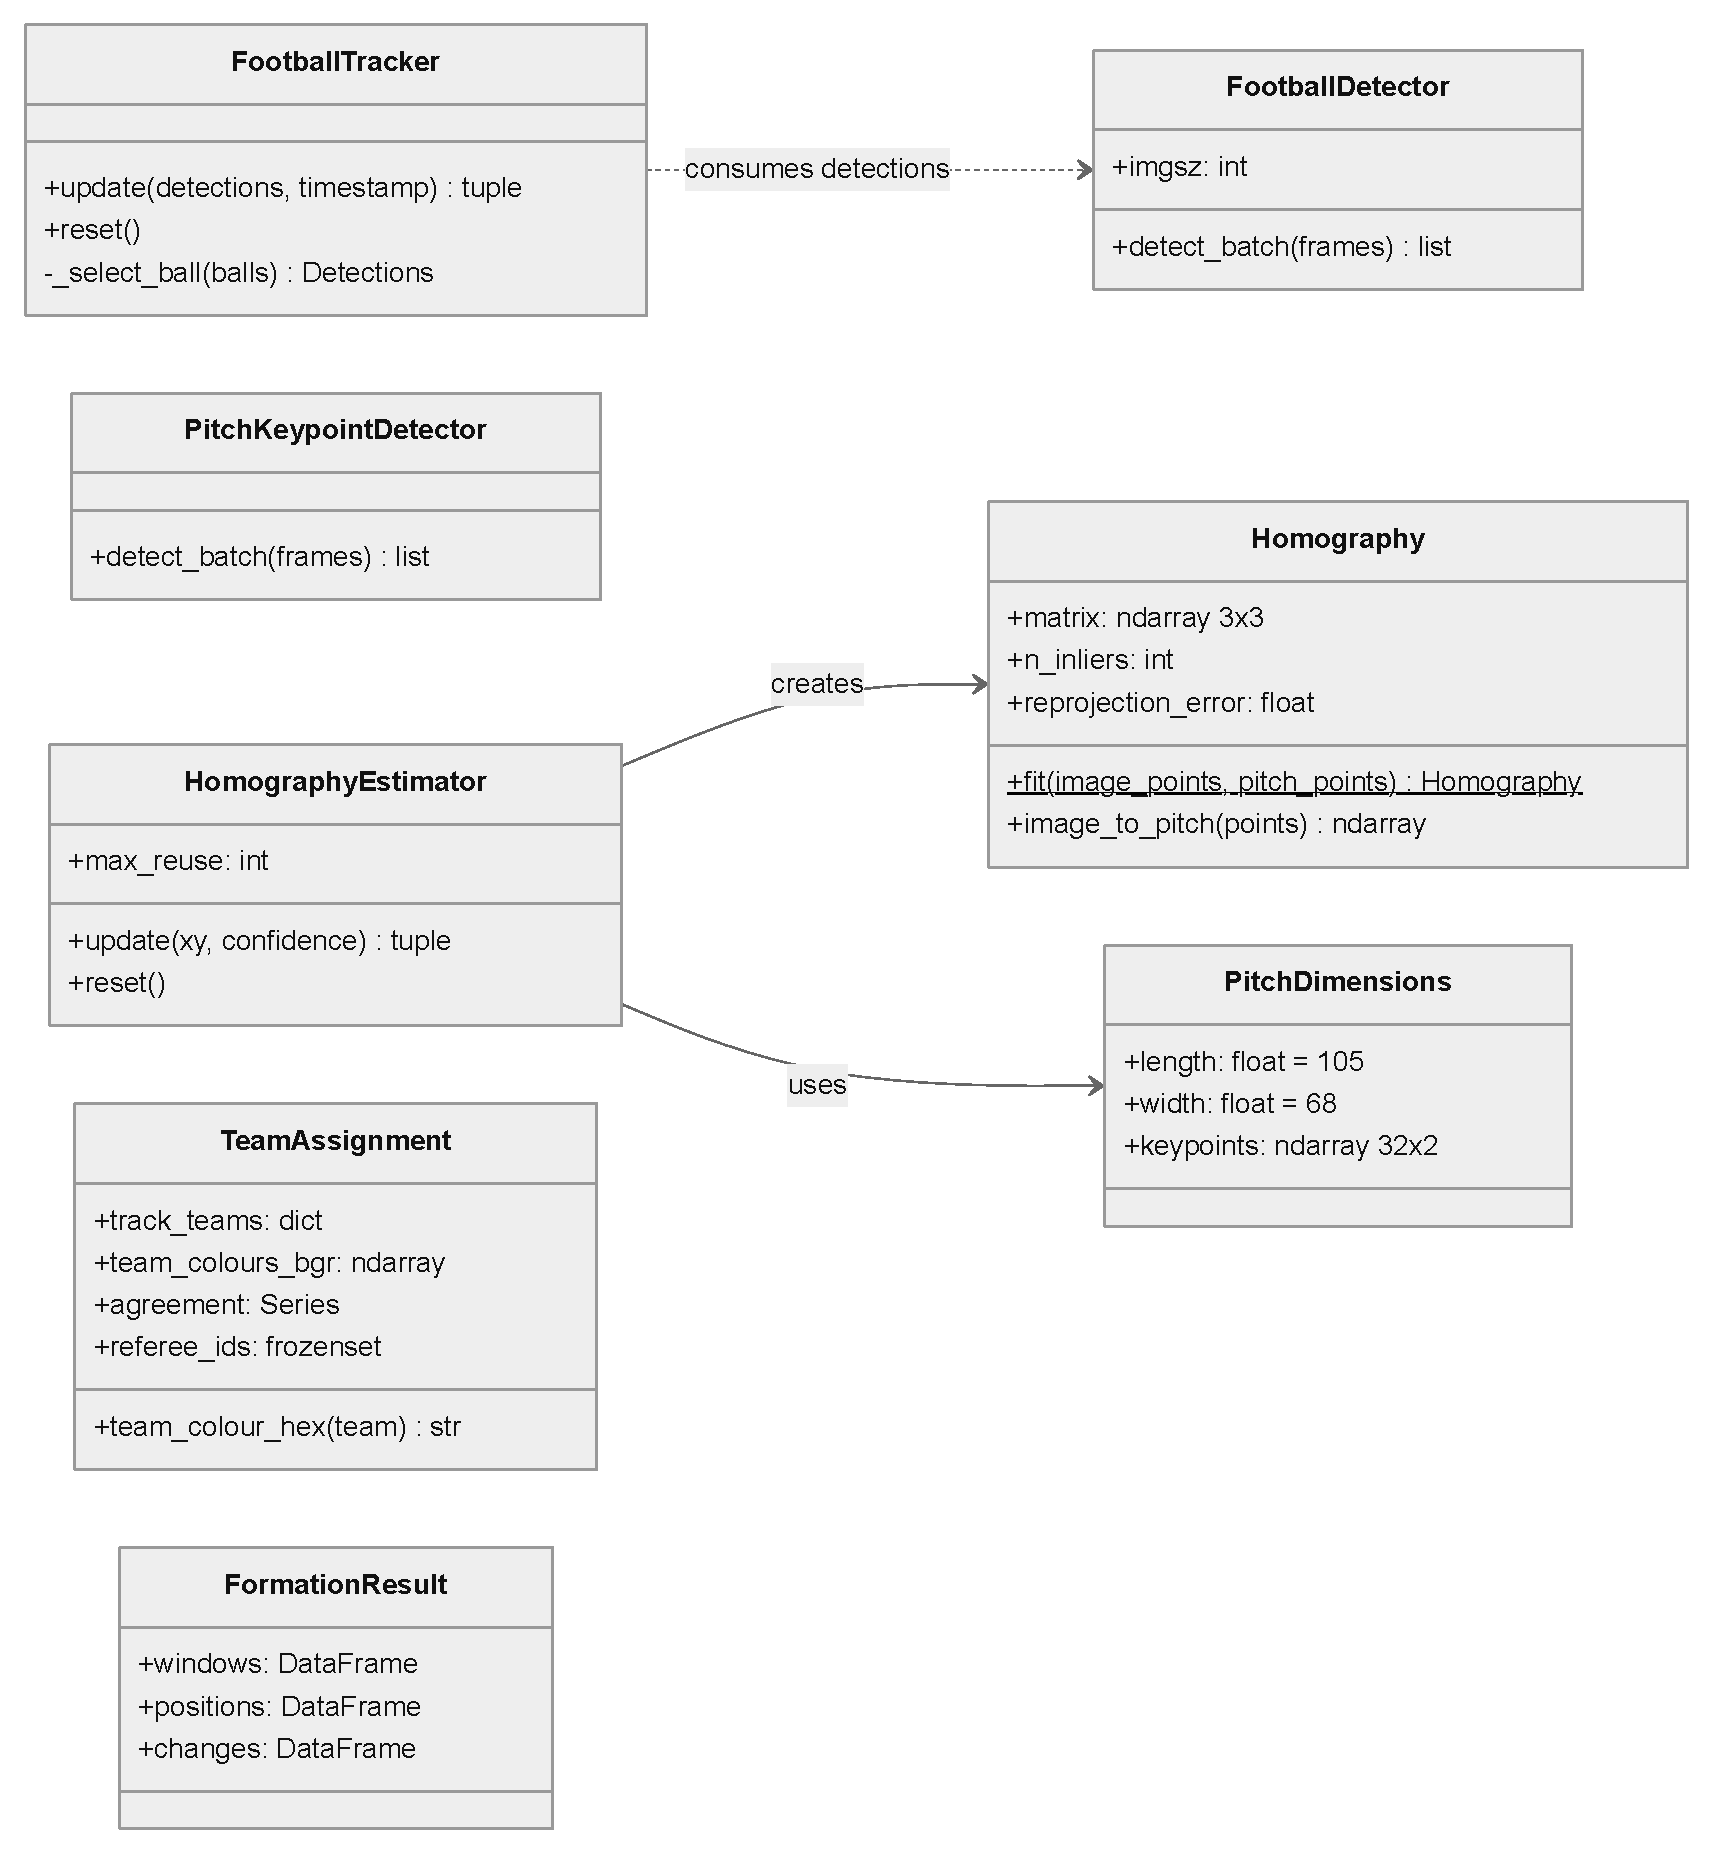
\includegraphics[width=\textwidth]{classes_worker}
	\caption{Main classes of the worker}
	\label{fig:classes}
\end{figure}

\subsection{Important functions}

\autoref{tab:worker-functions} gives the input, output and activity of the worker's key functions, in the order in which the pipeline calls them. ``Tracks'' means the tracks table, one row per detection per analysed frame.

\begin{longtable}{|p{0.22\textwidth}|p{0.30\textwidth}|p{0.39\textwidth}|}
	\hline
	\textbf{Function} & \textbf{Input $\rightarrow$ output} & \textbf{Activity} \\
	\hline
	\endhead
	\texttt{analyse} (worker.py) & queue job $\rightarrow$ \texttt{\{resultPath, playbackPath, summary\}} or \texttt{\{cancelled\}} & Returns a saved result if this run of the job has already finished; otherwise runs the analysis remotely or locally in a thread while watching for cancel notes, and saves a ``done'' note. \\
	\hline
	\texttt{run\_\allowbreak{}analysis} (pipeline.py) & video path, results path, playback path, progress callback, mode $\rightarrow$ summary dict & Runs every stage, measures peak RAM and GPU memory, writes the results file atomically and returns the summary with stage times and file sizes. \\
	\hline
	\texttt{make\_\allowbreak{}web\_\allowbreak{}video} (transcode.py) & source path, target path, frame callback $\rightarrow$ target path & Re-encodes to H.264 at a constant frame rate, one output frame per input frame, with ``faststart''. \\
	\hline
	\texttt{iter\_\allowbreak{}tracks} (tracker.py) & video, detector, stride $\rightarrow$ stream of \texttt{FrameTracks} & Reads frames in batches of four, detects, tracks people with ByteTrack, passes up to five ball candidates. \\
	\hline
	\texttt{iter\_\allowbreak{}homographies} (homography.py) & video, landmark detector, stride $\rightarrow$ stream of homographies & Detects landmarks and fits a RANSAC homography per frame, reusing the last one for up to 10 frames. \\
	\hline
	\texttt{smooth\_\allowbreak{}homographies} (homography.py) & homographies, image size, fps $\rightarrow$ homographies & Smooths the camera model over 1.5\,s via four fixed image points (\autoref{sec:camera-smoothing}). \\
	\hline
	\texttt{project\_\allowbreak{}tracks} (homography.py) & tracks, homographies, frame gap $\rightarrow$ tracks with \texttt{pitch\_\allowbreak{}x}, \texttt{pitch\_\allowbreak{}y} & Joins each row to the nearest homography and projects all foot points at once (\autoref{code:projection}). \\
	\hline
	\texttt{remove\_\allowbreak{}off\_\allowbreak{}pitch\_\allowbreak{}people} (cleanup.py) & tracks $\rightarrow$ tracks & Drops non-referee tracks whose median position is more than 0.5\,m outside the pitch. \\
	\hline
	\texttt{select\_\allowbreak{}ball} (cleanup.py) & tracks with ball candidates $\rightarrow$ tracks with at most one ball per frame & Follows the ball's path (\autoref{alg:ball}). \\
	\hline
	\texttt{extract\_\allowbreak{}jersey\_\allowbreak{}features} (clustering.py) & video, tracks $\rightarrow$ table of Lab colours per sample & Crops up to 10 samples per track in one pass over the video and measures the torso colour against the local grass. \\
	\hline
	\texttt{assign\_\allowbreak{}teams} (clustering.py) & tracks, colour samples $\rightarrow$ \texttt{TeamAssignment} & K-Means into two teams, removes referee-coloured tracks and clusters again, places goalkeepers by position. \\
	\hline
	\texttt{find\_\allowbreak{}referees} (clustering.py) & colour samples, roles, team colours, usual positions $\rightarrow$ set of track IDs & Learns the referee kit from the referee tracks and returns players (and goalkeepers outside both boxes) that wear it (\autoref{eq:referee}). \\
	\hline
	\texttt{add\_\allowbreak{}team\_\allowbreak{}column} (clustering.py) & tracks, assignment $\rightarrow$ tracks with \texttt{team}, \texttt{role} & Adds each row's team and role; relabels the found referees. \\
	\hline
	\texttt{stitch\_\allowbreak{}tracks} (cleanup.py) & tracks $\rightarrow$ tracks with new IDs & Joins broken pieces with the Hungarian algorithm and renumbers from 1. \\
	\hline
	\texttt{smooth\_\allowbreak{}positions} (trajectories.py) & tracks $\rightarrow$ tracks & One-second centred rolling mean per person; raw values kept. \\
	\hline
	\texttt{interpolate\_\allowbreak{}ball} (trajectories.py) & tracks $\rightarrow$ tracks with filled ball rows & Fills ball gaps of up to one second linearly; marks the new rows. \\
	\hline
	\texttt{detect\_\allowbreak{}formations} (clustering.py) & tracks $\rightarrow$ \texttt{FormationResult} & Per team and 5-second window: average positions, template matching, hysteresis and the 20-second stability rule. \\
	\hline
	\texttt{match\_\allowbreak{}formation} (clustering.py) & $(n, 2)$ positions $\rightarrow$ cost per formation & Hungarian assignment of players to the slots of each template (\autoref{code:matching}). \\
	\hline
	\texttt{assign\_\allowbreak{}positions} (positions.py) & tracks, formations $\rightarrow$ label per row & Slots of the main formation per window, smoothed per track, unique per frame; GK and REF for goalkeepers and referees. \\
	\hline
	\texttt{team\_\allowbreak{}shape} (metrics.py) & tracks $\rightarrow$ table per frame and team & Outfield players, hull area, width, depth and centroid. \\
	\hline
	\texttt{player\_\allowbreak{}stats} (metrics.py) & tracks, grouping columns $\rightarrow$ table per group & Distance, time visible, average speed and one-second top speed, per track or per team and position. \\
	\hline
	\texttt{heatmap} (metrics.py) & $x$, $y$ arrays $\rightarrow$ $14 \times 21$ grid of shares & Share of positions in each pitch cell. \\
	\hline
	\texttt{run\_\allowbreak{}remote\_\allowbreak{}analysis} (remote.py) & GPU address, token, video, outputs, callback, mode, stop check $\rightarrow$ summary & Uploads in 50\,MB pieces, starts the job, relays progress, cancels on request, downloads the outputs. \\
	\hline
	\caption{Important functions of the worker}
	\label{tab:worker-functions}
\end{longtable}

\subsection{Job processing}

\texttt{worker.\allowbreak{}py} creates a BullMQ \texttt{Worker} with a concurrency of one. The neural networks already use every CPU core, so two analyses at once would only make both slower. The worker registers under a unique name with host name and process ID, which lets the API's health check count workers, and holds a job lock of 120 seconds. If a worker crashes, its lock expires and BullMQ hands the job out again.

The analysis is slow, synchronous code. Run directly in the asynchronous event loop, it would block the loop, the lock would not be renewed and BullMQ would wrongly consider the job stalled. The worker therefore runs the analysis in a separate thread (\texttt{asyncio.\allowbreak{}to\_\allowbreak{}thread}), and progress callbacks from that thread are handed back to the event loop with \texttt{run\_\allowbreak{}coroutine\_\allowbreak{}threadsafe}. Progress is throttled: an update is only forwarded when the integer percentage or the stage text changes. The results file is written atomically, first to a temporary file that then replaces the target in one rename, so the API can never serve a half-written file. Before writing, any remaining \texttt{NaN} or infinity is replaced with \texttt{null} and counted in the log, so one bad value cannot fail a whole analysis.

\subsection{Surviving a sleeping computer}
\label{sec:sleep}

During the long-video runs, my laptop went to sleep while the second half was being analysed on the GPU. The log showed the worker checking the GPU job 28 times a minute until 04:25, then nothing until 05:33. The GPU finished the job in the meantime, but when the laptop woke up, BullMQ saw that the job's lock had not been renewed for over an hour, treated the job as stalled and handed it out again. The worker downloaded the finished results and then started the whole 48-minute analysis a second time; the database never recorded the first completion.

Making sure the laptop stays awake solved that session, but not the weakness. When an analysis finishes, the worker now saves a small note next to the results (\texttt{results/<matchId>.\allowbreak{}done.\allowbreak{}json}) with a fingerprint of the job run and the summary. The fingerprint is the job ID together with the job's creation time: a job handed out again after a stall keeps both, while a deliberate re-analysis creates a new job with a new creation time. When a job starts and finds a note with its own fingerprint, and the result files exist, the worker returns the saved summary at once instead of analysing again. A unit test hands the same job to the worker twice and checks that the analysis runs once, and that a real re-analysis still runs.

\subsection{The remote GPU service}

The optional GPU service (\texttt{gpu\_\allowbreak{}server.\allowbreak{}py}) is a small FastAPI application that runs the same pipeline on a machine with an NVIDIA GPU. It loads the models once at start-up. Every request must carry the shared secret as a Bearer token, and the service refuses to start with a token shorter than 16 characters. I kept the queue worker on the main server and moved only the computation (\autoref{fig:gpu-sequence}). The GPU service never touches the database, the queue or the storage, so it needs no access to the platform's network, and the main server never has to be reachable from the internet.

\begin{figure}[H]
	\centering
	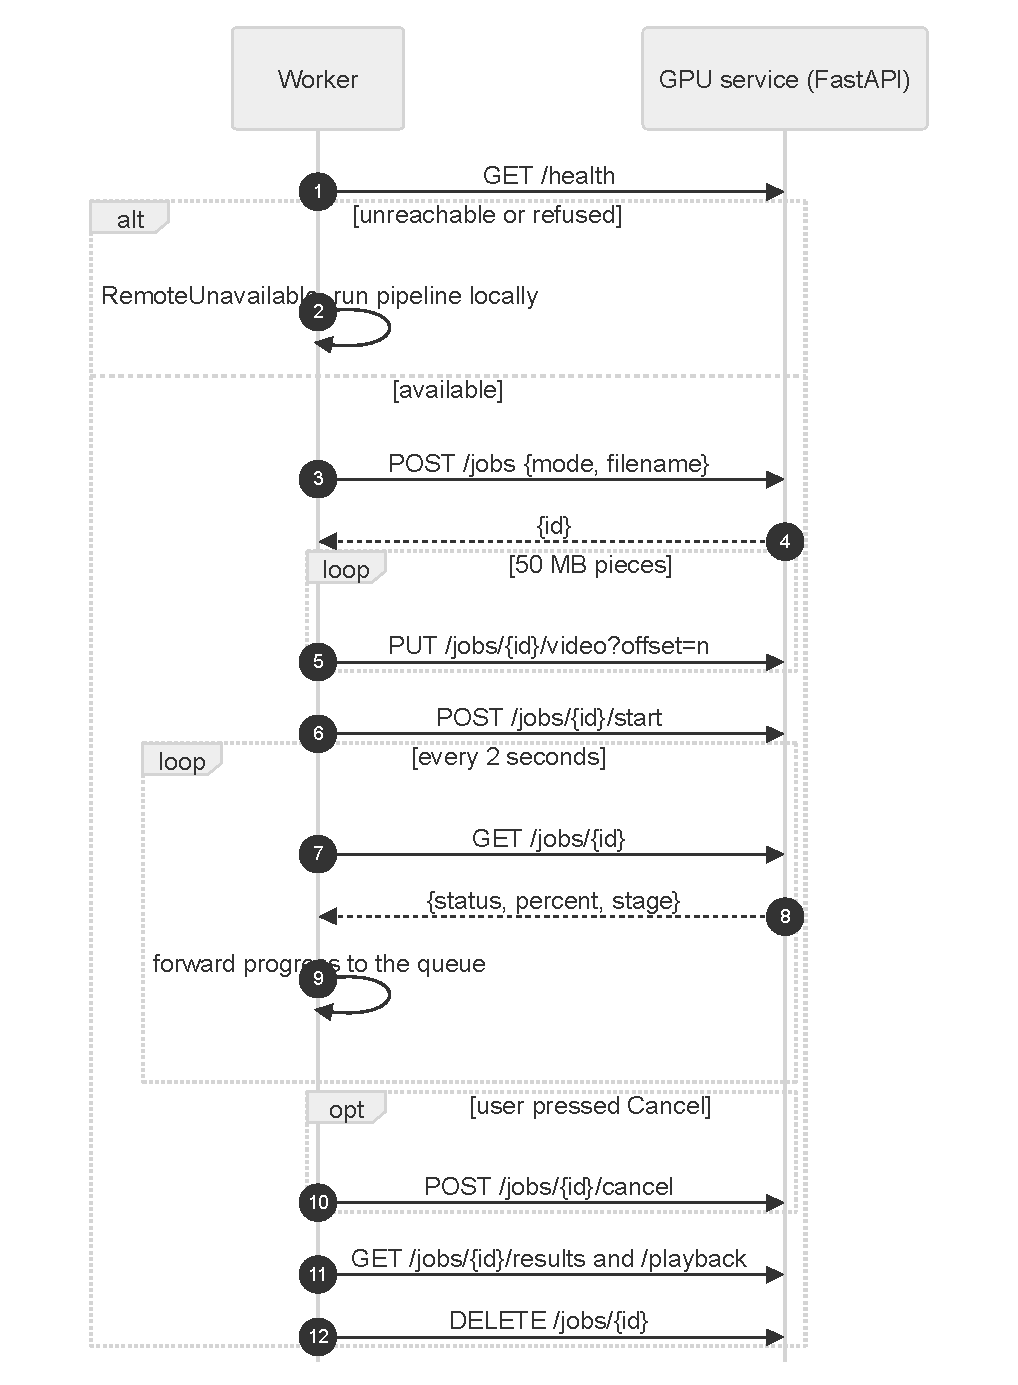
\includegraphics[width=0.75\textwidth]{gpu_sequence}
	\caption{Interaction between the worker and the remote GPU service}
	\label{fig:gpu-sequence}
\end{figure}

The first version uploaded the video in one request, which was fine for 20\,MB clips. A full half is over 500\,MB, and RunPod's HTTP proxy may refuse a request body of that size, so the protocol became three steps: \texttt{POST /jobs} creates an empty job, \texttt{PUT /jobs/\{id\}/video?offset=n} appends one piece of 50\,MB, and \texttt{POST /jobs/\{id\}/start} queues the analysis. Each piece carries its offset, so a piece that is sent twice after a network error is recognised and ignored, and a lost piece is retried up to three times. The 516\,MB first half uploaded in about a minute. The worker also stops waiting after four hours instead of two, enough for a 50\,fps half on a slower GPU.

The client in \texttt{remote.\allowbreak{}py} distinguishes two kinds of failure. \texttt{Remote\allowbreak{}Unavailable} means the service could not be reached or refused the job before any work started; the worker then analyses the video locally. \texttt{Remote\allowbreak{}Analysis\allowbreak{}Error} means the service failed during the job, and the attempt fails as usual and is retried.

\section{The frontend}

\subsection{Structure}

The dashboard in \texttt{frontend/src/} is a single-page application in React 19 and TypeScript, bundled by Vite. Its components form the tree in \autoref{fig:components}, and \autoref{tab:frontend-modules} lists them.

\begin{landscape}
	\begin{figure}
		\centering
		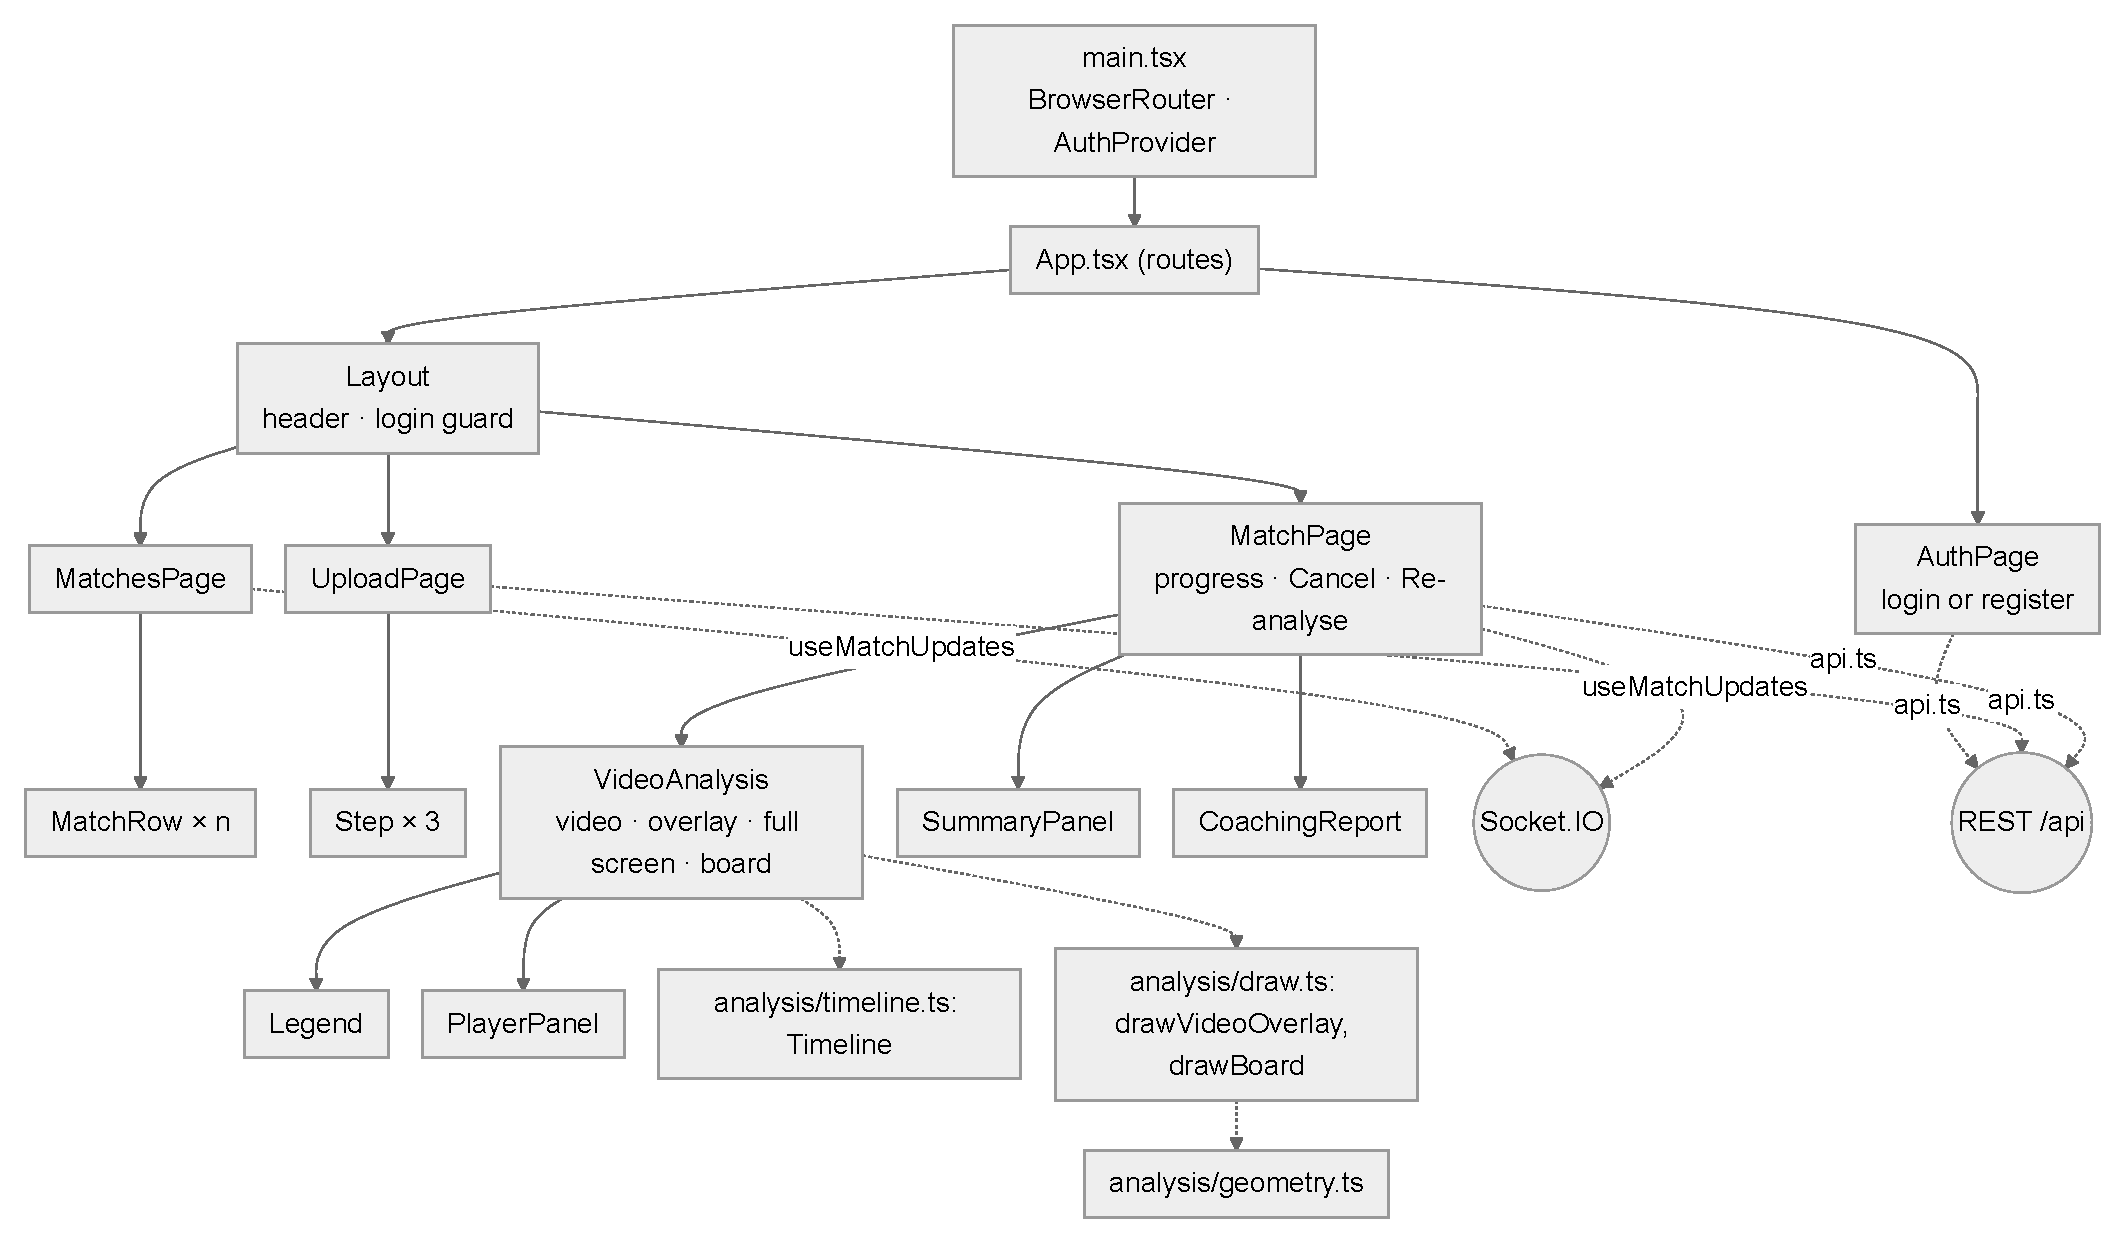
\includegraphics[width=\linewidth,height=0.86\textheight,keepaspectratio]{frontend_components}
		\caption{Component structure of the dashboard}
		\label{fig:components}
	\end{figure}
\end{landscape}

\begin{longtable}{|p{0.24\textwidth}|p{0.68\textwidth}|}
	\hline
	\textbf{Component or module} & \textbf{Responsibility} \\
	\hline
	\endhead
	\texttt{main.\allowbreak{}tsx}, \texttt{App.\allowbreak{}tsx} & Mount the application with the router and the authentication provider; define the routes. \\
	\hline
	\texttt{auth.\allowbreak{}tsx} & \texttt{AuthProvider} and \texttt{useAuth()}: the logged-in user, shared through React context; checks the session with \texttt{/auth/me} on start. \\
	\hline
	\texttt{api.\allowbreak{}ts} & Every REST call; \texttt{ApiError} with message and status; \texttt{uploadMatch()} with upload progress. \\
	\hline
	\texttt{useMatchUpdates.\allowbreak{}ts} & Hook that opens the Socket.IO connection and calls a callback for every \texttt{match:updated} event. \\
	\hline
	\texttt{Layout} & Header and navigation for logged-in pages; sends visitors to the log-in page. \\
	\hline
	\texttt{AuthPage} & Log-in and registration form, one component with two modes. \\
	\hline
	\texttt{MatchesPage}, \texttt{MatchRow} & Match list with live progress and delete confirmation. \\
	\hline
	\texttt{UploadPage}, \texttt{Step} & File by click or drag and drop, title, mode, upload progress. \\
	\hline
	\texttt{MatchPage}, \texttt{SummaryPanel} & Loads the match and its results; progress with Cancel, failure and cancelled notes, the analysis, the summary tab, Re-analyse. \\
	\hline
	\texttt{VideoAnalysis} & Video, overlay canvas, controls, full screen, layer buttons, tactical board, formations, tabs, \texttt{PlayerPanel}. \\
	\hline
	\texttt{CoachingReport} & Loads, generates and renders the Markdown report. \\
	\hline
	\texttt{analysis/timeline.\allowbreak{}ts} & \texttt{Timeline}: where everyone is at any moment, by interpolation; position labels. \\
	\hline
	\texttt{analysis/geometry.\allowbreak{}ts} & Applying and blending homographies, convex hull, fitting a picture into a box. \\
	\hline
	\texttt{analysis/draw.\allowbreak{}ts} & Drawing the video overlay and the board; finding the player under a click. \\
	\hline
	\texttt{components/ui.\allowbreak{}tsx} & Shared elements: button, card, status note, progress bar, error box, spinner, statistic. \\
	\hline
	\caption{Main components and modules of the dashboard}
	\label{tab:frontend-modules}
\end{longtable}

\subsection{Routing and navigation}

\autoref{tab:routes} and \autoref{fig:navigation} show the pages and how the user moves between them. The protected pages are nested inside \texttt{Layout}, which waits for the session check and redirects to \texttt{/login} when nobody is logged in. Unknown addresses redirect to the match list.

\begin{table}[H]
	\centering
	\begin{tabular}{|p{0.2\textwidth}|p{0.24\textwidth}|p{0.47\textwidth}|}
		\hline
		\textbf{Path} & \textbf{Page} & \textbf{Access} \\
		\hline
		\texttt{/login} & \texttt{AuthPage} (log in) & Public; logged-in users are sent to \texttt{/}. \\
		\hline
		\texttt{/register} & \texttt{AuthPage} (register) & Public; logged-in users are sent to \texttt{/}. \\
		\hline
		\texttt{/} & \texttt{MatchesPage} & Logged-in users. \\
		\hline
		\texttt{/upload} & \texttt{UploadPage} & Logged-in users. \\
		\hline
		\texttt{/matches/:id} & \texttt{MatchPage} & The logged-in owner of the match. \\
		\hline
	\end{tabular}
	\caption{Routes of the dashboard}
	\label{tab:routes}
\end{table}

\begin{figure}[H]
	\centering
	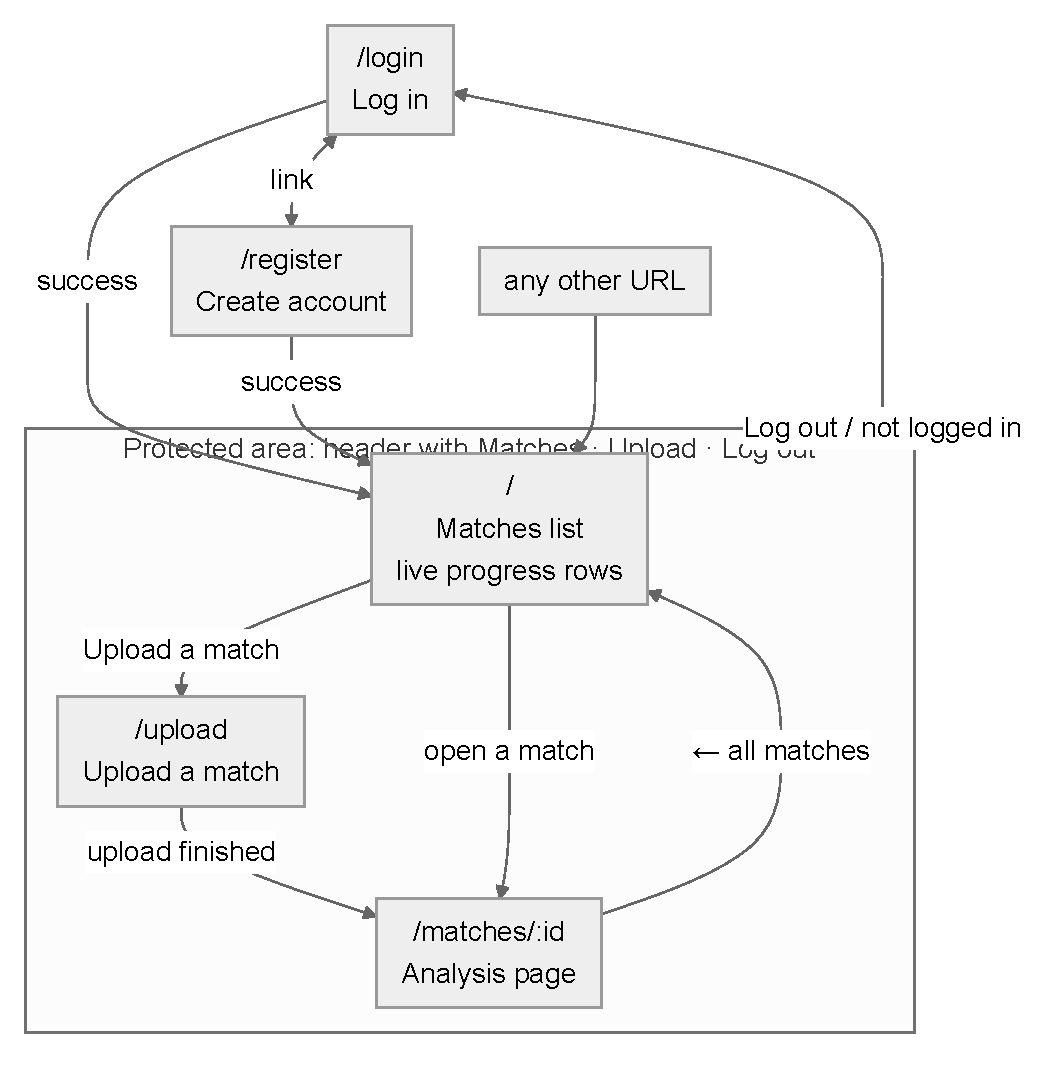
\includegraphics[width=0.75\textwidth]{navigation}
	\caption{Navigation between the pages}
	\label{fig:navigation}
\end{figure}

\subsection{State and live updates}

The dashboard uses React's own state (\texttt{useState}, \texttt{useEffect}) and one context for the logged-in user; no global state library was needed. The session cookie is HTTP-only, so the frontend cannot read it and learns whether the user is logged in from \texttt{/auth/me}. Pages subscribe to live updates with \texttt{use\allowbreak{}Match\allowbreak{}Updates(callback)}. The hook keeps the latest callback in a ref, so the WebSocket opens once per page and does not reconnect on every render. When a match becomes \texttt{COMPLETED}, the match page downloads the results. They are stored together with the completion time they belong to, so after a re-analysis stale results are never combined with new match data.

\subsection{Synchronising the overlays with the video}
\label{sec:overlay-sync}

Keeping the drawings on the players in every frame was the main difficulty of the frontend, and four techniques work together. First, the overlay is redrawn for every displayed frame with \texttt{request\allowbreak{}Video\allowbreak{}Frame\allowbreak{}Callback}~\cite{rvfc}, which reports the exact media time of the frame on screen; the \texttt{timeupdate} event, which I used first, lags up to a quarter of a second behind, and the markers visibly trailed the players. Browsers without the API fall back to \texttt{request\allowbreak{}Animation\allowbreak{}Frame}.

Second, the worker analyses only every 2nd or 4th frame, but the video shows every frame, so \texttt{Timeline.\allowbreak{}stateAt(t)} finds the analysed frames before and after $t$ by binary search and interpolates boxes and pitch positions between them. It never interpolates across a gap longer than three strides, such as a camera cut.

Third, paths and heatmaps are defined on the pitch, but the camera moves. For every frame the results contain the pitch-to-image homography; \texttt{applyHomography} projects pitch points into the current frame (\autoref{code:apply}), and between analysed frames the two matrices are blended. Points behind the camera ($w \le 0$) are skipped. A heatmap therefore appears painted on the grass and stays there while the camera pans, and since the worker smooths the camera model (\autoref{sec:camera-smoothing}), the paths no longer jump when a new camera update arrives.

Fourth, the canvases are redrawn directly in the frame callback, outside React. React state only holds things that change rarely (layer switches, the selection, the displayed time), and the drawing code reads the current switches through refs; re-rendering the component tree 25 to 50 times a second would be far too slow. The canvases are sized to their on-screen size times the device pixel ratio, so the drawings stay sharp, and a \texttt{ResizeObserver} redraws them when the layout changes, which also covers entering full screen.

\begin{lstlisting}[language=TypeScript, caption={Projecting a pitch point into the current video frame (from \texttt{frontend/src/analysis/geometry.\allowbreak{}ts})}, label={code:apply}]
export function applyHomography(h: number[], x: number, y: number): Point | null {
  const w = h[6] * x + h[7] * y + h[8];
  if (w <= 1e-9) return null;          // behind the camera
  return [(h[0] * x + h[1] * y + h[2]) / w, (h[3] * x + h[4] * y + h[5]) / w];
}
\end{lstlisting}

\subsection{The analysis modules}

\autoref{tab:frontend-functions} gives the inputs, outputs and activity of the functions in \texttt{analysis/}, which contain all the overlay logic.

\begin{longtable}{|p{0.24\textwidth}|p{0.30\textwidth}|p{0.37\textwidth}|}
	\hline
	\textbf{Function} & \textbf{Input $\rightarrow$ output} & \textbf{Activity} \\
	\hline
	\endhead
	\texttt{new Timeline} (timeline.ts) & results file $\rightarrow$ timeline & Sorts the frames by time, indexes each frame's people by track ID, remembers whether the file has position labels (version 3). \\
	\hline
	\texttt{Timeline.\allowbreak{}indexAt} & time $\rightarrow$ index of the last analysed frame at or before it, or $-1$ & Binary search over the frame times. \\
	\hline
	\texttt{Timeline.\allowbreak{}stateAt} & time in seconds $\rightarrow$ \texttt{FrameState} (people with box, foot, pitch position, label and selection key; ball; camera matrix) & Interpolates boxes, pitch positions, ball and camera matrix between the neighbouring analysed frames; empty inside long gaps. \\
	\hline
	\texttt{Timeline.\allowbreak{}trail} & track ID, time, seconds $\rightarrow$ pitch points, oldest first & Collects one person's positions over the last seconds (the 4-second movement path). \\
	\hline
	\texttt{Timeline.\allowbreak{}ballTrail} & time, seconds $\rightarrow$ pitch points & The ball's recent positions; stops at the first frame without a ball, so no line crosses the pitch after a gap. \\
	\hline
	\texttt{Timeline.\allowbreak{}fullPath} & position (or track) ID $\rightarrow$ list of path pieces & Every position of a selection over the video, split wherever another player takes over or the player is out of view. \\
	\hline
	\texttt{applyHomography} (geometry.ts) & $3 \times 3$ matrix, $x$, $y$ $\rightarrow$ image point or \texttt{null} & Projects a pitch point into the frame (\autoref{code:apply}); \texttt{null} behind the camera. \\
	\hline
	\texttt{lerpHomography} & two matrices, $\alpha$ $\rightarrow$ matrix & Element-wise blend for moments between analysed frames. \\
	\hline
	\texttt{convexHull} & points $\rightarrow$ hull points & Andrew's monotone chain; used for the team shape. \\
	\hline
	\texttt{fitContain} & source size, box size $\rightarrow$ scale and offset & Where the video sits inside its box, so canvas and video pixels line up. \\
	\hline
	\texttt{draw\allowbreak{}Video\allowbreak{}Overlay} (draw.ts) & canvas, size, results, timeline, frame state, layers, selection $\rightarrow$ drawing & Draws heatmap, team shape, paths, players with labels and the ball onto the video canvas, in this order. \\
	\hline
	\texttt{drawBoard} & canvas, size, results, timeline, frame state, layers, selection, options $\rightarrow$ drawing & Draws the chalk pitch, heatmap, static path, shapes, paths, people and ball on the board; also used for the small pitch of the \emph{Player} tab. \\
	\hline
	\texttt{personAt} & results, frame state, canvas size, click position $\rightarrow$ selection key or \texttt{null} & Finds the person whose box is nearest to a click on the video, within 25 pixels. \\
	\hline
	\texttt{personOnBoard} & the same for the board $\rightarrow$ selection key or \texttt{null} & Finds the person nearest to a click on the board. \\
	\hline
	\caption{Functions of the frontend analysis modules}
	\label{tab:frontend-functions}
\end{longtable}

\subsection{Event handlers}

\begin{longtable}{|p{0.25\textwidth}|p{0.26\textwidth}|p{0.40\textwidth}|}
	\hline
	\textbf{Handler} & \textbf{Input $\rightarrow$ output} & \textbf{Activity} \\
	\hline
	\endhead
	\texttt{AuthPage.\allowbreak{}handleSubmit} & form submit event $\rightarrow$ navigation to \texttt{/}, or error text & Stops the browser's own submit, calls \texttt{login} or \texttt{register}, shows the server's message on failure. \\
	\hline
	\texttt{UploadPage.\allowbreak{}chooseFile} & \texttt{File} $\rightarrow$ chosen file and title & Stores the file, clears old errors, suggests a title from the file name if none is typed. \\
	\hline
	\texttt{UploadPage.\allowbreak{}handleDrop} & drag event $\rightarrow$ chosen file & Stops the browser from opening the file and passes it to \texttt{chooseFile}. \\
	\hline
	\texttt{UploadPage.\allowbreak{}handleSubmit} & form submit event $\rightarrow$ navigation to the new match, or error text & Uploads with progress (\texttt{uploadMatch}), then opens the match page. \\
	\hline
	\texttt{MatchRow.\allowbreak{}handleDelete} & click on \emph{Yes} $\rightarrow$ row removed, or error text & Deletes the match through the API and removes it from the list. \\
	\hline
	\texttt{MatchPage.\allowbreak{}reanalyse} & click $\rightarrow$ updated match (queued) & Queues the analysis again and shows the returned match. \\
	\hline
	\texttt{MatchPage.\allowbreak{}cancel} & click $\rightarrow$ updated match (cancelled or cancelling) & Asks for confirmation, calls \texttt{/cancel} and shows the returned match. \\
	\hline
	\texttt{useMatchUpdates} callback & pushed match $\rightarrow$ new page state & Replaces the match on the page, or in the list, or adds a new one. \\
	\hline
	\texttt{VideoAnalysis.\allowbreak{}onOverlayClick} & mouse event on the video $\rightarrow$ selection changed, or play/pause & Finds the person under the click (\texttt{personAt}); an empty spot toggles playback. \\
	\hline
	\texttt{VideoAnalysis.\allowbreak{}onBoardClick} & mouse event on the board $\rightarrow$ selection changed & The same on the board (\texttt{personOnBoard}). \\
	\hline
	\texttt{VideoAnalysis.\allowbreak{}toggleSelection} & selection key or \texttt{null} $\rightarrow$ new selection, \emph{Player} tab & Selects a position, or clears the selection if it is already selected. \\
	\hline
	\texttt{VideoAnalysis.\allowbreak{}stepFrame} & $-1$ or $+1$ $\rightarrow$ video one frame back or forward & Pauses and seeks to the next frame, aiming slightly inside it so rounding cannot land on its neighbour. \\
	\hline
	\texttt{VideoAnalysis.\allowbreak{}togglePlay} & click $\rightarrow$ playing or paused & Starts or pauses the video. \\
	\hline
	\texttt{VideoAnalysis.\allowbreak{}toggleFullscreen} & click $\rightarrow$ full screen on or off & Puts the player block (video, drawings, controls) into full screen, or leaves it. \\
	\hline
	\texttt{fullscreenchange} listener & browser event $\rightarrow$ \texttt{fullscreen} state & Keeps the button and the layout right when the user leaves full screen with Esc. \\
	\hline
	Frame callback (\texttt{request\allowbreak{}Video\allowbreak{}Frame\allowbreak{}Callback}) & displayed frame's media time $\rightarrow$ redrawn canvases & Computes \texttt{stateAt} for that time and redraws the overlay and the board. \\
	\hline
	\texttt{CoachingReport.\allowbreak{}generate} & click $\rightarrow$ report text, or error text & Requests a new report, shows a spinner meanwhile, then the Markdown or the error. \\
	\hline
	\caption{Important event handlers of the dashboard}
	\label{tab:handlers}
\end{longtable}

\subsection{User interface design}

The first version of the dashboard used rounded cards, an emerald accent and a dark gradient, the default look of many generated interfaces, and my supervisor's feedback was that it looked like one. I redesigned it around the idea of a coach's tactics board: a dark pitch-green background with faint mowing stripes, chalk-white text and dashed lines, an amber accent, IBM Plex fonts, and handwritten Kalam notes for statuses and hints (``ready \checkmark'', ``Drop a video here''). The match list became rows instead of a grid of cards, the upload page a numbered three-step form, and the summary a side-by-side comparison table. On the tactical board, Team A is drawn as circles and Team B as crosses, as on a chalkboard, while the video overlay keeps the real kit colours so that the drawing matches the shirts. Interactive elements have accessible labels, destructive actions need a confirmation, and every asynchronous action shows its state and disables its button against double submission.

\section{Security}

\autoref{tab:security} lists the threats I considered and how the platform answers each.

\begin{table}[H]
	\centering
	\begin{tabular}{|p{0.28\textwidth}|p{0.62\textwidth}|}
		\hline
		\textbf{Threat} & \textbf{Measure} \\
		\hline
		Stolen password database & Passwords are stored only as bcrypt hashes with a salt per password~\cite{owasp}. \\
		\hline
		Session theft by injected scripts & The session token lives in an HTTP-only cookie that page scripts cannot read; React escapes all rendered text. \\
		\hline
		Forged requests from other sites & The cookie uses \texttt{SameSite=Lax}, and only the dashboard's own origin is allowed. \\
		\hline
		Access to other users' data & Every match query filters by the owner; other users' matches answer ``not found'', so their IDs cannot be probed. \\
		\hline
		Malicious uploads & Extension, type and the file's first bytes are checked; files get random names and a size limit. \\
		\hline
		Paths outside the storage & Every stored path is resolved and must stay inside the storage folder. \\
		\hline
		Invalid input & All request bodies and settings are validated with Zod. \\
		\hline
		Leaked secrets & Secrets live only in \texttt{.env}, which Git ignores; the language model receives statistics only. \\
		\hline
	\end{tabular}
	\caption{Security measures}
	\label{tab:security}
\end{table}

\section{Implementation decisions}

The code was typed throughout: TypeScript for the API and dashboard, type hints and dataclasses for the worker, and a database client which was automatically generated by the schema. When the output format of the results changed, the compiler would flag all places in the dashboard that were reading them.

Because I stream the data (i.e., video frames are pulled into memory in batch sizes, uploads directly to disk, the GPU upload is done piece-by-piece and the video player loads with range requests), memory remained relatively stable. A full half peaked at 3.6--4.4\,GB of RAM. I use Pandas and NumPy operations to process tracking data, as opposed to using Python loops, and I operate on whole columns. A half contains approximately 840,000 detections. All of the steps after pitch mapping combined took less than 3 minutes.

Each threshold in the pipeline has a name constant defined in \texttt{config.py} and a comment describing its value and when it was measured and on what data, therefore, if I want to run another experiment, I simply need to change one line. Comments describe why something is happening. All generic code is shared: there is one drawing function that can be used to draw both the board and player tab, there is one statistics function that can work either per track or per position, and the same \texttt{run\_\allowbreak{}analysis()} function will work whether a local or a GPU analysis is being performed.

There is an expectation of errors occurring (i.e., jobs are retried, results are written atomically, values that cannot be stored in JSON are replaced before writing, the GPU will fall-back to local analysis, and if a job is cancelled then no partially-written files will remain).


\cleardoublepage

\chapter{Testing}
\label{ch:testing}

\section{Test strategy}

In the first version of this thesis only the worker had automated tests, and the system tests were a list of steps I carried out by hand before each demonstration. That was not enough: a change to the queue or to the results format could break the platform without any test noticing.

The testing now works on five levels, and the first four run on every push in the CI pipeline (\autoref{sec:cicd}). Static checks come first: the TypeScript compiler checks the API and the dashboard, and oxlint lints the dashboard. White-box unit tests then check the worker's algorithms with constructed data whose correct result is known (43 tests) and the dashboard's overlay mathematics (23 tests). The backend's 42 API tests send real HTTP requests to the application, which talks to a real PostgreSQL test database and Redis. The 11 black-box system tests treat the whole platform in Docker as a browser would, through nginx, the REST API and the WebSocket, and include a real analysis. The fifth level is measurement: an accuracy check against hand-annotated frames, the analysis of the five demo clips and of two full halves, and processing-time comparisons.

A change that breaks any of the first four levels cannot be published as a Docker image, because the images job only runs after all of them pass.

\section{Unit tests of the worker}

The worker's tests are in \texttt{worker/tests/} and run with \texttt{python -m pytest} in about 10 seconds. They need neither videos nor model files: a known camera matrix is used to project pitch landmarks into a synthetic image, a red or lime shirt is painted on grass, a player is made to run in a straight line. Parametrised tests repeat a check for every formation. Most of the tests written after the first version are regression tests: each reproduces a defect found on real footage, so it cannot return silently. \autoref{tab:worker-tests} lists them; all 43 pass.

\begin{longtable}{|p{0.42\textwidth}|p{0.05\textwidth}|p{0.43\textwidth}|}
	\hline
	\textbf{Test} & \textbf{Cases} & \textbf{What is checked} \\
	\hline
	\endhead
	\multicolumn{3}{|l|}{\textit{Homography} (\texttt{test\_\allowbreak{}homography.\allowbreak{}py})} \\
	\hline
	\texttt{pitch\_\allowbreak{}keypoints\_\allowbreak{}match\_\allowbreak{}standard\_\allowbreak{}dimensions} & 1 & The 32 landmarks span exactly 0--105\,m and 0--68\,m. \\
	\hline
	\texttt{fit\_\allowbreak{}recovers\_\allowbreak{}the\_\allowbreak{}true\_\allowbreak{}mapping} & 1 & From 8 exact pairs all are inliers, the error is below 1\,mm, new points are projected right. \\
	\hline
	\texttt{fit\_\allowbreak{}ignores\_\allowbreak{}a\_\allowbreak{}wrong\_\allowbreak{}keypoint} & 1 & A landmark moved by 470\,px is rejected by RANSAC (\autoref{code:unit-test}). \\
	\hline
	\texttt{collinear\_\allowbreak{}keypoints\_\allowbreak{}are\_\allowbreak{}rejected} & 1 & Four points on the halfway line give no homography. \\
	\hline
	\texttt{project\_\allowbreak{}tracks\_\allowbreak{}puts\_\allowbreak{}feet\_\allowbreak{}on\_\allowbreak{}the\_\allowbreak{}pitch} & 1 & A foot at the image of the centre spot lands at (52.5, 34.0)\,m. \\
	\hline
	\texttt{exported\_\allowbreak{}matrices\_\allowbreak{}are\_\allowbreak{}finite\_\allowbreak{}when\_\allowbreak{}last\_\allowbreak{}entry\_\allowbreak{}is\_\allowbreak{}zero} & 1 & Regression: no \texttt{NaN} when the last matrix element is 0. \\
	\hline
	\texttt{smoothing\_\allowbreak{}removes\_\allowbreak{}a\_\allowbreak{}one\_\allowbreak{}frame\_\allowbreak{}wobble\_\allowbreak{}but\_\allowbreak{}follows\_\allowbreak{}a\_\allowbreak{}camera\_\allowbreak{}pan} & 1 & A 5\,m wobble in one frame disappears, a steady pan is still followed. \\
	\hline
	\multicolumn{3}{|l|}{\textit{Teams, formations and positions} (\texttt{test\_\allowbreak{}clustering.\allowbreak{}py}, \texttt{test\_\allowbreak{}positions.\allowbreak{}py})} \\
	\hline
	\texttt{shirt\_\allowbreak{}colour\_\allowbreak{}is\_\allowbreak{}measured\_\allowbreak{}with\_\allowbreak{}local\_\allowbreak{}grass} & 2 & A red and a lime shirt on grass are measured within 5 Lab units. \\
	\hline
	\texttt{fixed\_\allowbreak{}green\_\allowbreak{}range\_\allowbreak{}loses\_\allowbreak{}green\_\allowbreak{}kits} & 1 & Documents the old defect: a fixed green range removes the lime shirt. \\
	\hline
	\texttt{formation\_\allowbreak{}templates\_\allowbreak{}have\_\allowbreak{}ten\_\allowbreak{}outfield\_\allowbreak{}players} & 9 & Every template has 10 slots. \\
	\hline
	\texttt{noisy\_\allowbreak{}formation\_\allowbreak{}is\_\allowbreak{}recognised} & 9 & Each formation, scaled to a $35 \times 50$\,m shape with 1.5\,m noise per player, is matched to the right template. \\
	\hline
	\texttt{slot\_\allowbreak{}names\_\allowbreak{}match\_\allowbreak{}the\_\allowbreak{}template\_\allowbreak{}order} & 1 & Position names come out in template order (right to left per line). \\
	\hline
	\texttt{a\_\allowbreak{}player\_\allowbreak{}wearing\_\allowbreak{}the\_\allowbreak{}referee\_\allowbreak{}kit\_\allowbreak{}is\_\allowbreak{}found} & 1 & A ``player'' in the referees' colour is found as a referee. \\
	\hline
	\texttt{a\_\allowbreak{}goalkeeper\_\allowbreak{}in\_\allowbreak{}their\_\allowbreak{}box\_\allowbreak{}stays\_\allowbreak{}a\_\allowbreak{}goalkeeper} & 1 & Regression: a goalkeeper in an unusual kit inside the box is not turned into a referee; one in midfield is. \\
	\hline
	\multicolumn{3}{|l|}{\textit{Clean-up} (\texttt{test\_\allowbreak{}cleanup.\allowbreak{}py})} \\
	\hline
	\texttt{people\_\allowbreak{}standing\_\allowbreak{}off\_\allowbreak{}the\_\allowbreak{}pitch\_\allowbreak{}are\_\allowbreak{}removed\_\allowbreak{}but\_\allowbreak{}not\_\allowbreak{}a\_\allowbreak{}throw\_\allowbreak{}in} & 1 & A coach 3\,m off the pitch is removed; a winger stepping out briefly and an assistant referee stay. \\
	\hline
	\texttt{spare\_\allowbreak{}ball\_\allowbreak{}off\_\allowbreak{}the\_\allowbreak{}pitch\_\allowbreak{}is\_\allowbreak{}ignored\_\allowbreak{}and\_\allowbreak{}the\_\allowbreak{}ball\_\allowbreak{}path\_\allowbreak{}is\_\allowbreak{}followed} & 1 & With a rolling ball, a sharper spare ball off the pitch and a distant object, the rolling ball is chosen in every frame. \\
	\hline
	\texttt{penalty\_\allowbreak{}spot\_\allowbreak{}is\_\allowbreak{}not\_\allowbreak{}taken\_\allowbreak{}as\_\allowbreak{}the\_\allowbreak{}ball} & 1 & A confident ``ball'' on the penalty spot loses to a real one. \\
	\hline
	\texttt{two\_\allowbreak{}pieces\_\allowbreak{}of\_\allowbreak{}one\_\allowbreak{}player\_\allowbreak{}are\_\allowbreak{}joined\_\allowbreak{}and\_\allowbreak{}renumbered} & 1 & Two nearby pieces are joined, a distant one is not, IDs start at 1. \\
	\hline
	\multicolumn{3}{|l|}{\textit{Trajectories, metrics and export} (\texttt{test\_\allowbreak{}export.\allowbreak{}py}, \texttt{test\_\allowbreak{}metrics.\allowbreak{}py})} \\
	\hline
	\texttt{non\_\allowbreak{}finite\_\allowbreak{}numbers\_\allowbreak{}become\_\allowbreak{}null} & 1 & \texttt{NaN} and infinity become \texttt{null} and the atomic write succeeds. \\
	\hline
	\texttt{short\_\allowbreak{}ball\_\allowbreak{}gaps\_\allowbreak{}are\_\allowbreak{}interpolated} & 1 & A ball seen in frames 0 and 6 is filled in at frames 2 and 4. \\
	\hline
	\texttt{smoothing\_\allowbreak{}keeps\_\allowbreak{}raw\_\allowbreak{}positions\_\allowbreak{}and\_\allowbreak{}reduces\_\allowbreak{}jitter} & 1 & A $\pm 1$\,m zig-zag becomes an average step below 0.5\,m. \\
	\hline
	\texttt{steady\_\allowbreak{}run\_\allowbreak{}gives\_\allowbreak{}the\_\allowbreak{}true\_\allowbreak{}speed} & 1 & A 7\,m/s run gives 25.2\,km/h and the right distance. \\
	\hline
	\texttt{one\_\allowbreak{}position\_\allowbreak{}jump\_\allowbreak{}does\_\allowbreak{}not\_\allowbreak{}create\_\allowbreak{}a\_\allowbreak{}fake\_\allowbreak{}sprint} & 1 & Regression: a 0.35\,m jump keeps the top speed below 27\,km/h. \\
	\hline
	\texttt{tracks\_\allowbreak{}shorter\_\allowbreak{}than\_\allowbreak{}a\_\allowbreak{}second\_\allowbreak{}have\_\allowbreak{}no\_\allowbreak{}top\_\allowbreak{}speed} & 1 & A track under one second gets no top speed. \\
	\hline
	\multicolumn{3}{|l|}{\textit{Queue worker and GPU client} (\texttt{test\_\allowbreak{}worker.\allowbreak{}py}, \texttt{test\_\allowbreak{}remote.\allowbreak{}py})} \\
	\hline
	\texttt{a\_\allowbreak{}job\_\allowbreak{}handed\_\allowbreak{}out\_\allowbreak{}again\_\allowbreak{}after\_\allowbreak{}sleep\_\allowbreak{}is\_\allowbreak{}not\_\allowbreak{}analysed\_\allowbreak{}twice} & 1 & Regression: the same job twice runs once; a re-analysis runs again. \\
	\hline
	\texttt{cancelling\_\allowbreak{}tells\_\allowbreak{}the\_\allowbreak{}gpu\_\allowbreak{}service\_\allowbreak{}to\_\allowbreak{}stop} & 1 & Against a pretend GPU service: cancel calls \texttt{/cancel} and downloads nothing. \\
	\hline
	\caption{Unit tests of the worker (test names without the \texttt{test\_\allowbreak{}} prefix)}
	\label{tab:worker-tests}
\end{longtable}

\begin{lstlisting}[language=Python, caption={A unit test of the RANSAC fit (from \texttt{worker/tests/test\_\allowbreak{}homography.\allowbreak{}py})}, label={code:unit-test}]
def test_fit_ignores_a_wrong_keypoint():
    pitch_points = PitchDimensions().keypoints[[0, 5, 13, 16, 9, 12, 30, 31]]
    image_points = to_image(pitch_points)
    image_points[3] += [400, -250]  # one badly detected landmark
    homography = Homography.fit(image_points, pitch_points)
    assert homography is not None and homography.n_inliers == len(pitch_points) - 1
\end{lstlisting}

\section{API tests of the backend}

The backend's tests in \texttt{backend/test/} use Vitest~\cite{vitest} and SuperTest~\cite{supertest}, which sends real HTTP requests to the Express application without starting a server. I decided against mocking the database: most bugs I had found in the API were about how routes, Prisma and BullMQ work together, and a mock would have hidden exactly those. The tests therefore run against a real PostgreSQL database, the normal one with \texttt{\_\allowbreak{}test} added to its name, which Prisma's migrations create before the first test. They use Redis database 1, so the real worker, which listens on database 0, never picks up a test upload, a temporary storage folder, and an upload limit of 1\,MB so that the ``too large'' test is fast. Before every test, the tables are emptied and the test queue is cleared, and the tests run one file at a time because they share the database. A SuperTest agent works like a browser: it keeps the log-in cookie between requests. The 42 tests (\autoref{tab:api-tests}) take about 30 seconds.

\begin{longtable}{|p{0.25\textwidth}|p{0.66\textwidth}|}
	\hline
	\textbf{Group} & \textbf{What is tested} \\
	\hline
	\endhead
	Registration (6) & Creates the account and logs in without returning the password; stores a bcrypt hash; refuses an existing e-mail regardless of case; refuses a short password, an invalid address and a missing name with a message naming the field. \\
	\hline
	Log-in and log-out (4) & Right password works; wrong password and unknown e-mail get the same answer; \texttt{/auth/me} knows the user until log-out; a forged cookie is rejected. \\
	\hline
	Uploading (7) & Only when logged in; stores the file, creates a queued match and a job whose ID is the match ID; refuses a missing file, non-video names and types, a text file disguised as \texttt{.\allowbreak{}mp4} (and deletes it), files over the limit, an unknown mode. \\
	\hline
	Other users' matches (1) & Every route, including cancel, answers 404 for another user's match; their list stays empty. \\
	\hline
	Rules during analysis (4) & Results and reports only after the analysis; no double queueing; no deleting while processing; re-analysis in another mode. \\
	\hline
	Deleting (1) & Removes the match, its waiting job and its video file. \\
	\hline
	Cancelling (4) & A queued analysis is cancelled at once and leaves the queue; a running one (a test worker holds the job) gets the cancel note in Redis; refused when nothing runs and for other users; a cancelled re-analysis returns to the earlier results. \\
	\hline
	Coaching report (10) & Reports ``not configured'' without Azure settings; eight measured kit colours get the right names; the model's input names colours and positions and contains no colour codes or ``Player \#''. \\
	\hline
	Platform (5) & The health check reaches the database and Redis; unknown API paths answer 404 in JSON; stored paths cannot leave the storage folder; files are recognised as videos by their first bytes. \\
	\hline
	\caption{API tests of the backend (number of tests in brackets)}
	\label{tab:api-tests}
\end{longtable}

\section{Unit tests of the dashboard}

The overlay mathematics lives in two pure modules, \texttt{geometry.\allowbreak{}ts} and \texttt{timeline.\allowbreak{}ts}, which have no dependency on React or the browser, so Vitest tests them directly with small hand-made results files. The 23 tests cover \texttt{applyHomography} (identity, scale and offset, perspective division, points behind the camera), \texttt{lerpHomography}, \texttt{convexHull} (outer points only, points on an edge, fewer than three points), \texttt{fitContain} for wide and tall boxes, and the \texttt{Timeline}: the exact state at an analysed frame, interpolation halfway between two, the ball with an unknown pitch position, never blending across a long gap, the movement path, the ball path that stops at a missing ball, \texttt{indexAt}, and, for version-3 results, position labels, REF for referees, blank labels for unknown positions and a position's path split where another player takes over.

\section{System tests}

The system tests in \texttt{tests/system/} test the running platform from the outside, through nginx on port 8080, exactly as a browser does: \texttt{httpx} for the REST API and \texttt{python-socketio} for the live updates. Nothing is mocked, so a passing run means that the frontend server, the API, the database, the queue and the worker really work together. In CI the system job starts the whole platform with Docker Compose and runs them; locally they run against the platform on the laptop in about 11 minutes, most of it a real CPU analysis of a 3-second clip. \autoref{tab:system-tests} lists them; all pass.

\begin{longtable}{|p{0.04\textwidth}|p{0.27\textwidth}|p{0.30\textwidth}|p{0.27\textwidth}|}
	\hline
	\textbf{\#} & \textbf{Test} & \textbf{Action} & \textbf{Expected and observed} \\
	\hline
	\endhead
	1 & Health check & GET \texttt{/api/health} & 200, database and Redis up, at least 1 worker \\
	\hline
	2 & Deep link & Open \texttt{/matches/<id>} directly & nginx serves the dashboard \\
	\hline
	3 & Unknown API path & GET \texttt{/api/nothing} & 404 with a JSON error \\
	\hline
	4 & Login required & GET \texttt{/api/matches} without cookie & 401 \\
	\hline
	5--6 & Invalid registrations & Short password; invalid e-mail & 400 naming the field \\
	\hline
	7 & Log-in and log-out & Register, \texttt{/auth/me}, log out, \texttt{/auth/me} & 201, 200, 204, 401 \\
	\hline
	8 & Non-videos refused & A text file, and a text file named \texttt{.\allowbreak{}mp4} & 400 for both \\
	\hline
	9 & Video without players & A real 2-second video of plain grass & First attempt fails, retry, then failed with ``No players were detected in this video'' \\
	\hline
	10 & Full analysis & Upload a 3-second Bundesliga clip in Quick mode and listen on the WebSocket & At least 5 live updates with rising progress up to 100; completed with both teams; results version 3 with position labels; video Range request answers 206; another user gets 404; re-analyse works; delete works \\
	\hline
	11 & Cancelling & Upload two clips; cancel the queued one, then the running one & Queued: cancelled at once. Running: ``Cancelling\dots'', then cancelled within 60\,s (observed: 4\,s); both can be deleted \\
	\hline
	\caption{System tests}
	\label{tab:system-tests}
\end{longtable}

The dashboard's drawing was checked by hand in Edge and Chrome, and the screenshots of \autoref{ch:user} were captured by a Playwright~\cite{playwright} script that walks through the same steps: playing, pausing and stepping frames with every layer and heatmap switched on, selecting players on the video and the board, entering and leaving full screen, generating the coaching report, and the cancel, failure and delete flows.

\section{Accuracy against hand-annotated frames}
\label{sec:accuracy}

The first version of the thesis judged correctness only by internal measures and by watching the overlays. For a quantitative check I annotated 20 frames by hand: four from each demo clip, at 15, 40, 65 and 90\,\% of its analysed frames. The script \texttt{tests/accuracy/extract\_\allowbreak{}frames.\allowbreak{}py} saves exactly the frames the worker analysed, and \texttt{annotate.\allowbreak{}html}, a small page I wrote for the purpose, lets the annotator click every person's feet with a label (Team 1, Team 2, goalkeeper or referee), the ball and visible pitch landmarks. A person whose feet are hidden behind another player is clicked where the feet would be; a person of whom only a head or an arm is visible is skipped. The 20 frames contain 466 annotated people.

\texttt{evaluate.\allowbreak{}py} then compares the annotations with the results files. Clicked feet are paired with detected foot points by the Hungarian algorithm, and a pair counts if it is closer than 35 pixels at 1080p. Team labels are compared under the better of the two possible assignments of ``Team 1'' and ``Team 2'' to the system's teams, per clip. The ball counts as found within 20 pixels. Clicked landmarks are projected onto the pitch with the frame's camera model and compared with their true position, and the clicked and detected feet of each matched pair are both projected onto the pitch to measure the position error in metres.

\begin{table}[H]
	\centering
	\begin{tabular}{|p{0.42\textwidth}|p{0.22\textwidth}|p{0.22\textwidth}|}
		\hline
		\textbf{Measure} & \textbf{Before clean-up} & \textbf{Final pipeline} \\
		\hline
		People found (recall) & 99.1\,\% & 98.3\,\% \\
		\hline
		Detections that are real people (precision) & 99.8\,\% & 100\,\% \\
		\hline
		Role correct (player, goalkeeper, referee) & 100\,\% & 99.8\,\% \\
		\hline
		Team correct & 99.5\,\% & 98.8\,\% \\
		\hline
		Ball found / reported when not visible & 18 of 20 / 0 & 18 of 20 / 0 \\
		\hline
		Player position error, median (90\,\%) & 0.61\,m (0.95\,m) & 0.59\,m (0.95\,m) \\
		\hline
		Landmark error, median (90\,\%) & 0.84\,m (3.03\,m) & 0.86\,m (3.12\,m) \\
		\hline
	\end{tabular}
	\caption{Accuracy on 20 hand-annotated frames (466 people)}
	\label{tab:accuracy}
\end{table}

The first run of the final pipeline showed a role accuracy of 98.7\,\%, and all six errors were goalkeepers that the new referee rule had turned into referees. That led to the rule that only goalkeepers outside both penalty areas are checked, after which the accuracy was 99.8\,\% with one goalkeeper still labelled referee because he stood outside his box at that moment. The recall fell from 99.1 to 98.3\,\% for a reason that is not an error: all seven ``missed'' people are in one clip, at the bottom edge of the image, and the frame shows that they are substitutes waiting at the halfway line next to the fourth official. I had annotated them as Team 1 because they wear the kit, but they are off the pitch, and removing them is what the clean-up is for. Without them, the recall is 458 of 459, or 99.8\,\%.

These numbers have clear limits. 20 frames and 466 people are a small sample, I made the annotations myself, and the clips are the broadcast footage the detection model was trained for, so the results are a best case for this kind of video rather than a guarantee for any camera. They also measure single frames: whether a player keeps the same identity over time is not covered, and that is exactly where the system is weakest.

\section{The five demo clips}

The five 30-second Bundesliga clips (25\,fps, $1920 \times 1080$) from the DFL Bundesliga Data Shootout~\cite{dfl} were re-analysed with the final pipeline in Standard mode on an NVIDIA L4 (\autoref{tab:clips}).

\begin{table}[H]
	\centering
	\footnotesize
	\setlength{\tabcolsep}{4pt}
	\begin{tabular}{|c|c|c|c|c|c|c|c|}
		\hline
		\textbf{Clip} & \textbf{Frames} & \textbf{Valid camera} & \textbf{Reproj.} & \textbf{Ball} & \textbf{Formations A / B} & \textbf{Top speed} & \textbf{Time} \\
		\hline
		1 & 374 & 100\,\% & 0.23\,m & 62\,\% & 3-4-3 / 5-3-2 & 23.8\,km/h & 39.8\,s \\
		\hline
		2 & 374 & 100\,\% & 0.24\,m & 71\,\% & 4-4-2 / 3-4-3 & 27.3\,km/h & 38.9\,s \\
		\hline
		3 & 375 & 100\,\% & 0.26\,m & 50\,\% & 4-3-3 / 4-4-2 & 28.8\,km/h & 36.5\,s \\
		\hline
		4 & 374 & 100\,\% & 0.22\,m & 69\,\% & 4-2-3-1 / 3-5-2 & 23.6\,km/h & 35.9\,s \\
		\hline
		5 & 375 & 100\,\% & 0.19\,m & 52\,\% & 5-3-2 / 4-2-3-1 & 27.6\,km/h & 35.7\,s \\
		\hline
	\end{tabular}
	\caption{Results of the five demo clips (Standard mode, NVIDIA L4)}
	\label{tab:clips}
\end{table}

A camera model was available in every analysed frame, with a mean reprojection error of 0.19--0.26\,m, small compared with the 5--15\,m spacing between players that matters tactically. Every formation window of every clip was classified, and with the 20-second stability rule no clip reports a formation change, which is plausible for 30 seconds of play. The team distances of 0.54--0.80\,km per 30 seconds for about ten visible outfield players correspond to 1.8--2.7\,m/s per player, a realistic pace. The highest top speed per clip is now 23.6--28.8\,km/h, typical sprint speeds; the 39.6\,km/h of the first version (\autoref{sec:metrics}) is gone. The ball was found in 50--71\,\% of the analysed frames, mostly missed in the air, behind players or blurred. Clip 1, analysed on the laptop CPU and on the GPU, gives the same formations; K-Means uses a fixed seed, so repeated runs give identical teams.

\section{Full halves}
\label{sec:long-videos}

My supervisor asked for at least one long video. I analysed two complete halves in Standard mode on a RunPod NVIDIA L4: the first half of Barcelona--Real Madrid (47:20, $1920 \times 1080$, 25\,fps, AV1, 516\,MB) and a half of PSG--Barcelona (48:14, $1280 \times 720$, 50\,fps, AV1, 434\,MB). Both are wide tactical-camera recordings. \autoref{tab:long-videos} gives the measurements and \autoref{fig:long-stages} shows where the time went.

\begin{table}[H]
	\centering
	\begin{tabular}{|p{0.36\textwidth}|p{0.25\textwidth}|p{0.25\textwidth}|}
		\hline
		& \textbf{Barcelona--Real Madrid} & \textbf{PSG--Barcelona} \\
		\hline
		Video & 47:20, 1080p, 25\,fps & 48:14, 720p, 50\,fps \\
		\hline
		Analysed frames & 35,500 & 36,174 \\
		\hline
		Processing time (GPU service) & 53.9\,min & 48.5\,min \\
		\hline
		\quad playback copy (CPU of the pod) & 15.2\,min & 11.0\,min \\
		\hline
		\quad detection and tracking & 31.7\,min & 30.9\,min \\
		\hline
		\quad pitch mapping & 4.3\,min & 3.9\,min \\
		\hline
		\quad teams, tactics, saving & 2.8\,min & 2.8\,min \\
		\hline
		Upload to the GPU / download & about 1 / 2\,min & about 1 / 1\,min \\
		\hline
		Peak RAM / peak GPU memory & 3.6\,GB / 1.5\,GB & 4.4\,GB / 1.8\,GB \\
		\hline
		Results file / playback copy & 54\,MB / 1.2\,GB & 52\,MB / 0.65\,GB \\
		\hline
		Valid camera / reprojection error & 100\,\% / 0.24\,m & 100\,\% / 0.26\,m \\
		\hline
		Ball found & 57\,\% & 48\,\% \\
		\hline
		Main formations A / B; changes & 4-1-4-1 / 4-3-3; 14 & 4-1-4-1 / 3-5-2; 6 \\
		\hline
		Distance per team & 56.9 / 54.8\,km & 63.0 / 58.8\,km \\
		\hline
	\end{tabular}
	\caption{Analysis of two full halves (Standard mode, NVIDIA L4)}
	\label{tab:long-videos}
\end{table}

\begin{figure}[H]
	\centering
	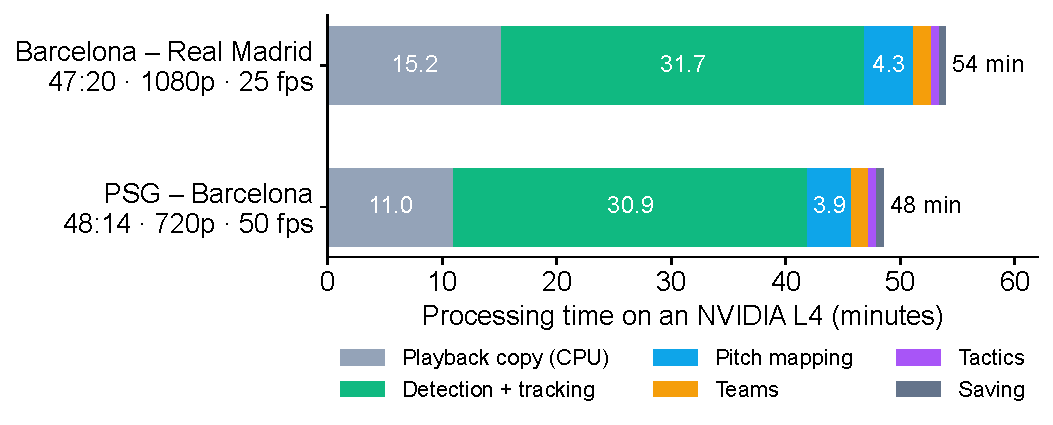
\includegraphics[width=0.9\textwidth]{long_video_stages}
	\caption{Processing time of the two halves per pipeline stage}
	\label{fig:long-stages}
\end{figure}

Processing took slightly more than real time on the L4, about 1.1 times the video length for the 25\,fps half and 1.0 times for the 50\,fps one, thanks to the frame-rate-aware stride. Detection and tracking dominate with about 31 minutes each. The second largest share, 11--15 minutes, is the H.264 playback copy, which runs on the pod's CPU. An earlier run of the first half on a different pod (a slice of an RTX PRO 6000 with a faster CPU) made the copy in 6.4 minutes and finished the whole half in 35 minutes, so the choice of machine matters as much as the GPU model. The GPU itself was barely used: at most 1.8\,GB of its 24\,GB of memory, so a much smaller and cheaper GPU would do. Peak RAM stayed below 4.5\,GB because frames are streamed. The dashboard handled the 54\,MB results file and the 1.2\,GB video without changes: the results are fetched once, and the video seeks immediately thanks to Range requests.

The distances of 55--63\,km per team over 47--48 minutes correspond to about 5.5--6.3\,km per outfield player-equivalent, in line with what professional players run in a half. The per-position top speeds are less convincing: their medians are 34.5 and 35.1\,km/h and the highest is 40.3\,km/h, above what players reach. On a 30-second clip, the top speed is the best one-second average of one player; over a half, a position's top speed is the best second out of 47 minutes, over several players and every tracking error in between, and one wrongly joined track or a wrong position in a fast camera pan is enough to set it. For full halves the distances are meaningful, while the top speed would need a statistic that one bad second cannot set, for example a high percentile instead of the maximum.

More valuable than the numbers was what the halves revealed about the pipeline. Nearly all the changes described in \autoref{sec:pipeline} after the first version came from these two runs: the upload limit and the chunked GPU upload, analysing the H.264 copy because OpenCV could not seek in AV1, the frame-rate-aware stride, the colour threshold for small players, the removal of people off the pitch, the ball selection, the referee detection, the joining of tracks, the position labels, the formation stability rule, the camera smoothing, and the protection against analysing a job twice. None of them showed up on the 30-second clips.

\section{Efficiency}

\autoref{tab:times} and \autoref{fig:performance} compare the processing times on the laptop and on the cloud GPU. The analysis is dominated by the two neural networks, so the GPU makes a large difference: a 30-second clip in Standard mode takes about 25 minutes on the laptop's CPU and 36--40 seconds on an L4. With the upload of the video and the download of the results, the total is about 53 seconds, still 28 times faster.

\begin{table}[H]
	\centering
	\begin{tabular}{|p{0.30\textwidth}|p{0.18\textwidth}|p{0.20\textwidth}|p{0.18\textwidth}|}
		\hline
		\textbf{Job} & \textbf{Laptop CPU (i7-1255U)} & \textbf{Docker on the laptop} & \textbf{Cloud GPU (L4)} \\
		\hline
		3\,s clip, Quick & 44--75\,s & 93\,s (207\,s first job) & 5\,s \\
		\hline
		30\,s clip, Standard & about 25\,min & not measured & 36--40\,s \\
		\hline
		47\,min half, Standard & not practical & not practical & 48--54\,min \\
		\hline
	\end{tabular}
	\caption{Processing times}
	\label{tab:times}
\end{table}

\begin{figure}[H]
	\centering
	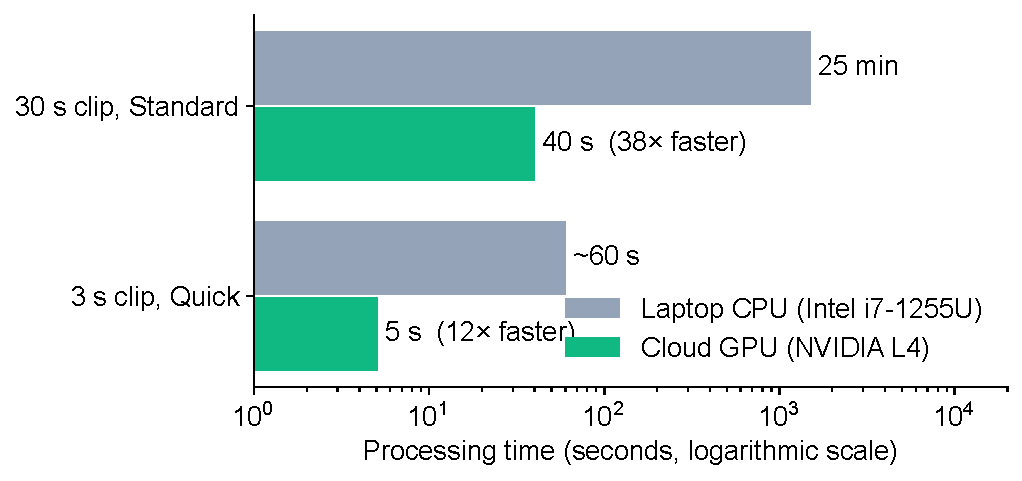
\includegraphics[width=0.85\textwidth]{performance}
	\caption{Processing time of the clips on the laptop CPU and on the cloud GPU (logarithmic scale)}
	\label{fig:performance}
\end{figure}

Three observations shaped the implementation. The first job after a worker starts is slower because the models are loaded; caching them per process means later jobs do not pay this again. Inside Docker on Windows the analysis was slower than natively, because the containers run in a WSL 2 virtual machine with a limited share of processor and memory. And the laptop's own GPU, a GeForce MX550 with 2\,GB, was about twice as slow as its CPU for these large models, which is why the worker defaults to the CPU and GPU work went to a rented machine. Laptop memory was a constraint of its own: with 7.7\,GB of RAM and the Docker stack running, two local analyses at the same time failed with out-of-memory errors while I was preparing the clean-up steps, so all local experiments ran one at a time.

\section{Scalability}

Workers share nothing but the queue and the storage, and the queue gives each job to exactly one worker, so throughput grows with the number of workers. More workers start with \texttt{docker compose --profile app up -d --scale worker=N} or on other machines, which then need access to the same storage, for example a network file system or object storage. The GPU service is stateless apart from its running jobs and can run on several machines. The API is stateless except for the Socket.IO rooms; several API instances behind a load balancer would need the Socket.IO Redis adapter so that events reach users connected to another instance. Processing time and the results file grow linearly with the video length: about 54\,MB per half, about 110\,MB for a full match, which the dashboard still loads as one file but which a future version could load in segments.

\section{Problems found during testing}

\autoref{tab:lessons} lists the defects that testing uncovered and the changes they led to. The first group comes from the first version on the demo clips, the second from the full halves and the new tests.

\begin{longtable}{|p{0.45\textwidth}|p{0.46\textwidth}|}
	\hline
	\textbf{Problem found} & \textbf{Change} \\
	\hline
	\endhead
	Uploaded clips did not play in the browser: the dataset uses a codec browsers do not support. & New stage: an H.264 playback copy at a constant frame rate, which also keeps the overlays frame-exact. \\
	\hline
	Two of five clips failed with ``out of range float values: nan'': for some camera angles the last matrix element is nearly zero. & Matrices are normalised by their norm with a fixed sign; non-finite numbers become \texttt{null}; regression test. \\
	\hline
	A team in a lime kit was not recognised: the fixed green range removed the shirts too. & The grass colour is measured around each player and compared in Lab space; two tests. \\
	\hline
	Goalkeepers were often labelled ``player'' and joined an outfield team. & Roles per track (25\,\% goalkeeper detections suffice); goalkeepers assigned by position. \\
	\hline
	The progress bar sometimes jumped backwards. & Database updates of each match are chained. \\
	\hline
	A re-analysis was accepted but nothing happened: BullMQ ignores a job whose ID still exists. & The finished job is removed before the new one is added. \\
	\hline
	The health check showed 0 workers while the Python worker ran. & Workers are counted from Redis's client list, accepting both naming schemes. \\
	\hline
	A top speed of 39.6\,km/h on clip 3. & Top speed as the best one-second average; regression test. \\
	\hline
	The laptop GPU was slower than its CPU. & CPU by default; optional cloud GPU with fallback. \\
	\hline
	\multicolumn{2}{|l|}{\textit{Found on the full halves and by the new tests}} \\
	\hline
	The first half was just over the 500\,MB upload limit, and RunPod's proxy may refuse a request body of that size. & Limit raised to 1\,GB; GPU upload in 50\,MB pieces with offsets and retries. \\
	\hline
	OpenCV failed to seek in the AV1 halves (``Corrupt frame detected''). & All stages read the H.264 playback copy. \\
	\hline
	The 50\,fps half would take twice as long as needed. & Stride scaled with the frame rate. \\
	\hline
	Far players ($8 \times 17$\,px) got no shirt colour; most of a team had no team. & Minimum shirt pixels relative to the player's size. \\
	\hline
	Substitutes and staff on the sidelines were marked as players. & Tracks usually more than 0.5\,m off the pitch are removed; test. \\
	\hline
	The main referee was counted as a player. & Referee kit learned from the assistants; players in that colour become referees; tests. \\
	\hline
	Spare balls and the penalty spot were taken for the ball (12\,\% of positions off the pitch). & Several candidates per frame, ball path followed on the pitch (\autoref{alg:ball}); tests. \\
	\hline
	Player numbers climbed to 1,423 over a half. & Broken tracks joined (555 left), then position labels (11 per team). \\
	\hline
	282 formation changes in one half. & A new formation must last 20 seconds (14 changes). \\
	\hline
	Movement paths darted across the video. & Camera model smoothed over 1.5\,s; test. \\
	\hline
	The CI system test failed after the results format changed to version 3. & The test was updated and now also checks the position labels. \\
	\hline
	The referee rule turned six goalkeepers of the demo clips into referees (found by the accuracy check). & Goalkeepers are only checked outside both penalty areas; regression test. \\
	\hline
	After the laptop slept, the queue handed the finished second half out again, and it was analysed twice. & ``Done'' note per job run; test. \\
	\hline
	\caption{Problems found during testing and the resulting changes}
	\label{tab:lessons}
\end{longtable}

The most useful lesson was that every new kind of footage exposed problems the previous tests could not have found. The codec, the camera angles and the kit colours were specific to the first real clips, and the sidelines, the spare balls, the referee and the identity problem only appeared over a full half. The five 30-second clips had made the pipeline look finished. Testing on long, real footage early, and turning each defect into a test, would have saved me the most time.

\section{Limitations and future work}
\label{sec:limitations}

The largest limitation is the single camera. Only what the broadcast camera shows is analysed, and players cannot be identified over a match, which is why the labels follow positions. Tactical-camera footage of the whole pitch, several camera angles, or shirt numbers read from higher-resolution video would allow named players and per-player statistics.

Two weaknesses only show over long videos. When only part of a team is visible, the slot matching can shift labels between neighbouring positions, and a position's top speed over a half is the single best second, which one tracking error can set (\autoref{sec:long-videos}). A high percentile instead of the maximum, and labels smoothed over longer periods, would make both less sensitive to single errors.

Events are missing entirely: passes, shots, tackles and possession are not detected. The distance between the ball and the nearest players over time would be a first step towards estimating possession and passes. The ball itself is found in only about half of the analysed frames of a full half; a model trained for small, fast objects, or a higher detection resolution around the ball's last known position, would help.

Processing a full half takes about as long as watching it on an L4, and the playback copy is encoded on the CPU, not the GPU. Splitting a match into segments that several workers analyse in parallel, and loading the results in time segments, would make full matches practical. The platform also runs on one machine; object storage instead of a shared folder, the Socket.IO Redis adapter and an orchestrator such as Kubernetes would spread it over several, and exporting queue length, processing times and error rates to a monitoring system would allow alerting.

Finally, the evaluation is small. The accuracy check covers 20 frames that I annotated myself. A larger set annotated by several people, or sensor tracking data, would measure positions, teams and especially identities over time far more reliably.

\cleardoublepage

\chapter{Conclusion}
\label{ch:conclusion}

I set out to find how much of the tactical picture that professional clubs buy can be recovered from one broadcast camera, and to show it in a form a coach would use. Tactical Eye does this for short clips and for full halves. A user uploads a video, follows or cancels the analysis, and then sees every player labelled by position, the referees marked, paths, team shapes and heatmaps painted on the grass in sync with the video, next to a tactical board, the formations of both teams and an AI-written report. On 20 hand-annotated frames it found 98.3\,\% of the people with no false detections and placed them on the pitch with a median error of 0.59\,m, and 119 automated tests run on every change.

The biggest surprise was how little the 30-second test clips told me. On them the pipeline looked finished. The first full half broke that impression within an hour: coaches on the touchline became players, spare balls became the ball, the referee joined a team, the tracker handed out 1,423 identities, and the movement paths jumped across the screen. None of these was a bug in the usual sense; the design had simply never met a stoppage or a 47-minute camera pan. I had also expected the neural networks to be the hard part, but they were the most reliable component. The difficult problems were in the geometry and bookkeeping around them: a camera model that wobbles, a decoder that cannot seek, a queue that hands out a finished job again after a laptop sleeps.

If I started again, I would test on a full half in the first month, and I would write the API and system tests together with the first endpoints instead of months later. I would also design the results format for long videos from the start, so that a full match could be loaded in parts.

Most of the work ran on a laptop with 8\,GB of RAM and no usable GPU, which shaped many decisions: the queue, the cancel button, the rented GPUs (under USD 2 in total for all experiments) and the protection against analysing a job twice. With footage of the whole pitch, player identities and event detection, Tactical Eye could come close to the tools professional clubs use; even now it gives an amateur coach a view of their team's shape that until recently required a stadium tracking system.

\cleardoublepage

% Bibliography (mandatory)
\phantomsection
\addcontentsline{toc}{chapter}{\biblabel}
\printbibliography[title=\biblabel]
\cleardoublepage

% Lists of figures, tables, algorithms and code samples
\phantomsection
\addcontentsline{toc}{chapter}{\lstfigurelabel}
\listoffigures
\cleardoublepage

\phantomsection
\addcontentsline{toc}{chapter}{\lsttablelabel}
\listoftables
\cleardoublepage

\end{document}
